% **************************************************************************************************************
% A Classic Thesis Style
% An Homage to The Elements of Typographic Style
%
% Copyright (C) 2018 André Miede and Ivo Pletikosić
%
% If you like the style then I would appreciate a postcard. My address
% can be found in the file ClassicThesis.pdf. A collection of the
% postcards I received so far is available online at
% http://postcards.miede.de
%
% License:
% This program is free software; you can redistribute it and/or modify
% it under the terms of the GNU General Public License as published by
% the Free Software Foundation; either version 2 of the License, or
% (at your option) any later version.
%
% This program is distributed in the hope that it will be useful,
% but WITHOUT ANY WARRANTY; without even the implied warranty of
% MERCHANTABILITY or FITNESS FOR A PARTICULAR PURPOSE.  See the
% GNU General Public License for more details.
%
% You should have received a copy of the GNU General Public License
% along with this program; see the file COPYING.  If not, write to
% the Free Software Foundation, Inc., 59 Temple Place - Suite 330,
% Boston, MA 02111-1307, USA.
%
% PLEASE SEE ALSO THE AUTHORS' NOTE REGARDING THIS LICENSE
% IN THE DOCUMENTATION (ClassicThesis.pdf --> Chapter 1 / Chapter01.tex)
% **************************************************************************************************************
\RequirePackage{silence} % :-\
    \WarningFilter{scrreprt}{Usage of package `titlesec'}
    %\WarningFilter{scrreprt}{Activating an ugly workaround}
    \WarningFilter{titlesec}{Non standard sectioning command detected}
\documentclass[ twoside,openright,titlepage,numbers=noenddot,%1headlines,
                headinclude,footinclude,cleardoublepage=empty,abstract=on,
                BCOR=5mm,paper=b5,fontsize=11pt,
		dvipsnames
                ]{scrbook}

%********************************************************************
% Note: Make all your adjustments in here
%*******************************************************
% ****************************************************************************************************
% classicthesis-config.tex
% formerly known as loadpackages.sty, classicthesis-ldpkg.sty, and classicthesis-preamble.sty
% Use it at the beginning of your ClassicThesis.tex, or as a LaTeX Preamble
% in your ClassicThesis.{tex,lyx} with % ****************************************************************************************************
% classicthesis-config.tex
% formerly known as loadpackages.sty, classicthesis-ldpkg.sty, and classicthesis-preamble.sty
% Use it at the beginning of your ClassicThesis.tex, or as a LaTeX Preamble
% in your ClassicThesis.{tex,lyx} with % ****************************************************************************************************
% classicthesis-config.tex
% formerly known as loadpackages.sty, classicthesis-ldpkg.sty, and classicthesis-preamble.sty
% Use it at the beginning of your ClassicThesis.tex, or as a LaTeX Preamble
% in your ClassicThesis.{tex,lyx} with \input{classicthesis-config}
% ****************************************************************************************************
% If you like the classicthesis, then I would appreciate a postcard.
% My address can be found in the file ClassicThesis.pdf. A collection
% of the postcards I received so far is available online at
% http://postcards.miede.de
% ****************************************************************************************************


% ****************************************************************************************************
% 0. Set the encoding of your files. UTF-8 is the only sensible encoding nowadays. If you can't read
% äöüßáéçèê∂åëæƒÏ€ then change the encoding setting in your editor, not the line below. If your editor
% does not support utf8 use another editor!
% ****************************************************************************************************
\PassOptionsToPackage{utf8}{inputenc}
  \usepackage{inputenc}

\PassOptionsToPackage{T1}{fontenc} % T2A for cyrillics
  \usepackage{fontenc}


% ****************************************************************************************************
% 1. Configure classicthesis for your needs here, e.g., remove "drafting" below
% in order to deactivate the time-stamp on the pages
% (see ClassicThesis.pdf for more information):
% ****************************************************************************************************
\PassOptionsToPackage{
  b5paper=true,
  drafting=false,    % print version information on the bottom of the pages
  tocaligned=false, % the left column of the toc will be aligned (no indentation)
  dottedtoc=false,  % page numbers in ToC flushed right
  eulerchapternumbers=true, % use AMS Euler for chapter font (otherwise Palatino)
  linedheaders=false,       % chaper headers will have line above and beneath
  floatperchapter=true,     % numbering per chapter for all floats (i.e., Figure 1.1)
  eulermath=true,  % use awesome Euler fonts for mathematical formulae (only with pdfLaTeX)
  beramono=true,    % toggle a nice monospaced font (w/ bold)
  palatino=true,    % deactivate standard font for loading another one, see the last section at the end of this file for suggestions
  style=classicthesis % classicthesis, arsclassica
}{classicthesis}


% ****************************************************************************************************
% 2. Personal data and user ad-hoc commands (insert your own data here)
% ****************************************************************************************************
\newcommand{\myTitle}{Analysis of Markovian Population Models\xspace}
\newcommand{\mySubtitle}{Dissertation zur Erlangung des Grades des Doktors der Naturwissenschaften\xspace}
\newcommand{\myDegree}{Master of Science (MSc.)\xspace}
\newcommand{\myName}{Michael Backenköhler\xspace}
\newcommand{\myProf}{Prof.~Dr.~Verena Wolf\xspace}
\newcommand{\myOtherProf}{Prof.~Dr.~Luca Bortolussi\xspace}
\newcommand{\mySupervisor}{Prof.~Dr.~Verena Wolf\xspace}
\newcommand{\myFaculty}{Faculty of Maths and Informatics\xspace}
\newcommand{\myDepartment}{Saarland Informatics Campus\xspace}
\newcommand{\myUni}{Saarland University\xspace}
\newcommand{\myLocation}{Saarbrücken\xspace}
\newcommand{\myTime}{June 2022\xspace}
\newcommand{\myVersion}{\classicthesis}

% ********************************************************************
% Setup, finetuning, and useful commands
% ********************************************************************
\providecommand{\mLyX}{L\kern-.1667em\lower.25em\hbox{Y}\kern-.125emX\@}
\newcommand{\ie}{i.\,e.}
\newcommand{\Ie}{I.\,e.}
\newcommand{\eg}{e.\,g.}
\newcommand{\Eg}{E.\,g.}
% ****************************************************************************************************


% ****************************************************************************************************
% 3. Loading some handy packages
% ****************************************************************************************************
% ********************************************************************
% Packages with options that might require adjustments
% ********************************************************************
\PassOptionsToPackage{ngerman,american}{babel} % change this to your language(s), main language last
% Spanish languages need extra options in order to work with this template
%\PassOptionsToPackage{spanish,es-lcroman}{babel}
    \usepackage{babel}

\usepackage{csquotes}
\PassOptionsToPackage{%
  %backend=biber,bibencoding=utf8, %instead of bibtex
  backend=bibtex8,bibencoding=utf8,%
  language=auto,%
  %style=numeric-comp,%
  %style=alphabetic,
  style=authoryear-comp, % Author 1999, 2010
  bibstyle=authoryear,dashed=false, % dashed: substitute rep. author with ---
  sorting=nyt, % name, year, title
  maxbibnames=10, % default: 3, et al.
  %backref=true,%
  natbib=true % natbib compatibility mode (\citep and \citet still work)
}{biblatex}
    \usepackage{biblatex}


\PassOptionsToPackage{fleqn}{amsmath}       % math environments and more by the AMS
  \usepackage{amsmath}

% ********************************************************************
% General useful packages
% ********************************************************************
\usepackage{graphicx} %
\usepackage{scrhack} % fix warnings when using KOMA with listings package
\usepackage{xspace} % to get the spacing after macros right
\PassOptionsToPackage{printonlyused,smaller}{acronym}
  \usepackage{acronym} % nice macros for handling all acronyms in the thesis
  %\renewcommand{\bflabel}[1]{{#1}\hfill} % fix the list of acronyms --> no longer working
  %\renewcommand*{\acsfont}[1]{\textsc{#1}}
  %\renewcommand*{\aclabelfont}[1]{\acsfont{#1}}
  %\def\bflabel#1{{#1\hfill}}
  \def\bflabel#1{{\acsfont{#1}\hfill}}
  \def\aclabelfont#1{\acsfont{#1}}
% ****************************************************************************************************
%\usepackage{pgfplots} % External TikZ/PGF support (thanks to Andreas Nautsch)
%\usetikzlibrary{external}
%\tikzexternalize[mode=list and make, prefix=ext-tikz/]
% ****************************************************************************************************


% ****************************************************************************************************
% 4. Setup floats: tables, (sub)figures, and captions
% ****************************************************************************************************
\usepackage{tabularx} % better tables
  \setlength{\extrarowheight}{3pt} % increase table row height
\newcommand{\tableheadline}[1]{\multicolumn{1}{l}{\spacedlowsmallcaps{#1}}}
\newcommand{\myfloatalign}{\centering} % to be used with each float for alignment
\usepackage{subfig}
% ****************************************************************************************************


% ****************************************************************************************************
% 5. Setup code listings
% ****************************************************************************************************
\usepackage{listings}
%\lstset{emph={trueIndex,root},emphstyle=\color{BlueViolet}}%\underbar} % for special keywords
\lstset{language=[LaTeX]Tex,%C++,
  morekeywords={PassOptionsToPackage,selectlanguage},
  keywordstyle=\color{RoyalBlue},%\bfseries,
  basicstyle=\small\ttfamily,
  %identifierstyle=\color{NavyBlue},
  commentstyle=\color{Green}\ttfamily,
  stringstyle=\rmfamily,
  numbers=none,%left,%
  numberstyle=\scriptsize,%\tiny
  stepnumber=5,
  numbersep=8pt,
  showstringspaces=false,
  breaklines=true,
  %frameround=ftff,
  %frame=single,
  belowcaptionskip=.75\baselineskip
  %frame=L
}
% ****************************************************************************************************

\newcommand{\e}[2]{\ensuremath{ #1\!\times\hspace{-.5ex} 10^{#2} }}

\DeclareMathOperator*{\argmax}{arg\,max}
\DeclareMathOperator*{\argmin}{arg\,min}
\DeclareMathOperator*{\Var}{Var}
\DeclareMathOperator*{\COV}{Cov}

\newcommand{\expSym}{{E}}
\newcommand{\E}[1]{\ensuremath{\expSym\left(#1\right)}}
\newcommand{\prob}[1]{\ensuremath{\Pr\left(#1\right)}}
\newcommand{\T}{T}
\newcommand{\Cov}[2]{\ensuremath{\COV(#1, #2)}}

\usepackage{amsmath}
\usepackage{amssymb}
\usepackage{amsthm}
\usepackage{thmtools}
%\usepackage{graphicx}
% \usepackage{algorithm}



\newtheorem{model}{Model}{\bfseries}{\itshape }
\newtheorem*{model*}{Model}{\bfseries}{\itshape }

\usepackage[ruled,vlined,linesnumbered]{algorithm2e}
\usepackage{algpseudocode}
\usepackage{booktabs}
\usepackage{todonotes}
\usepackage{mathtools}

\usepackage{multirow}

\newcommand{\PreserveBackslash}[1]{\let\temp=\\#1\let\\=\temp}
\newcolumntype{C}[1]{>{\PreserveBackslash\centering}p{#1}}
\newcolumntype{R}[1]{>{\PreserveBackslash\raggedleft}p{#1}}
\newcolumntype{L}[1]{>{\PreserveBackslash\raggedright}p{#1}}

\def\modelautorefname{Model}
\def\algorithmautorefname{Algorithm}

\usepackage{adjustbox}

\usepackage{tikz}
\usetikzlibrary{mindmap,trees,backgrounds}

\newcommand{\turnto}[1]{\marginpar{$\hookrightarrow \text{page~\pageref{#1}}$}}
% \newcommand{\example}[1]{\paragraph{Example}
% #1\nopagebreak\begin{flushright}{\Large$\diamond$}\end{flushright}}

\newenvironment{example}
    {\paragraph{Example}}
    {\nopagebreak\hfill{\Large$\diamond$}


    }
\newenvironment{changemargin}[2]{%
\begin{list}{}{%
\setlength{\topsep}{0pt}%
\setlength{\leftmargin}{#1}%
\setlength{\rightmargin}{#2}%
\setlength{\listparindent}{\parindent}%
\setlength{\itemindent}{\parindent}%
\setlength{\parsep}{\parskip}%
}%
\item[]}{\end{list}}

\renewcommand{\vec}[1]{#1}



\usepackage[group-separator={,}]{siunitx}

\makeatletter
\def\toc@spacedlowsmallcaps#1{%
  \texorpdfstring{\noexpand\spacedlowsmallcaps{#1}}{#1}%
}
\xpatchcmd{\tocbasic@listhead}
  {\addxcontentsline{toc}{chapter}{##1}}
  {\addxcontentsline{toc}{chapter}{\toc@spacedlowsmallcaps{##1}}}
  {}{}
\makeatother

\makeatletter
\DeclareCiteCommand{\fullcite}
  {\defcounter{maxnames}{\blx@maxbibnames}%
    \usebibmacro{prenote}}
  {\usedriver
     {\DeclareNameAlias{sortname}{default}}
     {\thefield{entrytype}}}
  {\multicitedelim}
  {\usebibmacro{postnote}}
\DeclareCiteCommand{\footfullcite}[\mkbibfootnote]
  {\defcounter{maxnames}{\blx@maxbibnames}%
    \usebibmacro{prenote}}
  {\usedriver
     {\DeclareNameAlias{sortname}{default}}
     {\thefield{entrytype}}}
  {\multicitedelim}
  {\usebibmacro{postnote}}
\makeatother
%%
%% \usepackage{tocloft}
% \newcommand{\listlemmaname}{List of Models}
% \newlistof{model}{model}{\listmodelname}

% ****************************************************************************************************
% 7. Last calls before the bar closes
% ****************************************************************************************************
% ********************************************************************
% Her Majesty herself
% ********************************************************************
\usepackage{classicthesis}


% ********************************************************************
% Fine-tune hyperreferences (hyperref should be called last)
% ********************************************************************
\hypersetup{%
  %draft, % hyperref's draft mode, for printing see below
  colorlinks=true, linktocpage=true, pdfstartpage=3, pdfstartview=FitV,%
  % uncomment the following line if you want to have black links (e.g., for printing)
  %colorlinks=false, linktocpage=false, pdfstartpage=3, pdfstartview=FitV, pdfborder={0 0 0},%
  breaklinks=true, pageanchor=true,%
  pdfpagemode=UseNone, %
  % pdfpagemode=UseOutlines,%
  plainpages=false, bookmarksnumbered, bookmarksopen=true, bookmarksopenlevel=1,%
  hypertexnames=true, pdfhighlight=/O,%nesting=true,%frenchlinks,%
  urlcolor=CTurl, linkcolor=CTlink, citecolor=CTcitation, %pagecolor=RoyalBlue,%
  %urlcolor=Black, linkcolor=Black, citecolor=Black, %pagecolor=Black,%
  pdftitle={\myTitle},%
  pdfauthor={\textcopyright\ \myName, \myUni, \myFaculty},%
  pdfsubject={},%
  pdfkeywords={},%
  pdfcreator={pdfLaTeX},%
  pdfproducer={LaTeX with hyperref}%
}


% ********************************************************************
% Setup autoreferences (hyperref and babel)
% ********************************************************************
% There are some issues regarding autorefnames
% http://www.tex.ac.uk/cgi-bin/texfaq2html?label=latexwords
% you have to redefine the macros for the
% language you use, e.g., american, ngerman
% (as chosen when loading babel/AtBeginDocument)
% ********************************************************************
\makeatletter
\@ifpackageloaded{babel}%
  {%
    \addto\extrasamerican{%
      \renewcommand*{\figureautorefname}{Figure}%
      \renewcommand*{\tableautorefname}{Table}%
      \renewcommand*{\partautorefname}{Part}%
      \renewcommand*{\chapterautorefname}{Chapter}%
      \renewcommand*{\sectionautorefname}{Section}%
      \renewcommand*{\subsectionautorefname}{Section}%
      \renewcommand*{\subsubsectionautorefname}{Section}%
    }%
    \addto\extrasngerman{%
      \renewcommand*{\paragraphautorefname}{Absatz}%
      \renewcommand*{\subparagraphautorefname}{Unterabsatz}%
      \renewcommand*{\footnoteautorefname}{Fu\"snote}%
      \renewcommand*{\FancyVerbLineautorefname}{Zeile}%
      \renewcommand*{\theoremautorefname}{Theorem}%
      \renewcommand*{\appendixautorefname}{Anhang}%
      \renewcommand*{\equationautorefname}{Gleichung}%
      \renewcommand*{\itemautorefname}{Punkt}%
    }%
      % Fix to getting autorefs for subfigures right (thanks to Belinda Vogt for changing the definition)
      \providecommand{\subfigureautorefname}{\figureautorefname}%
    }{\relax}
\makeatother


% ********************************************************************
% Development Stuff
% ********************************************************************
\listfiles
%\PassOptionsToPackage{l2tabu,orthodox,abort}{nag}
%  \usepackage{nag}
%\PassOptionsToPackage{warning, all}{onlyamsmath}
%  \usepackage{onlyamsmath}


% ****************************************************************************************************
% 7. Further adjustments (experimental)
% ****************************************************************************************************
% ********************************************************************
% Changing the text area
% ********************************************************************
%\areaset[current]{312pt}{761pt} % 686 (factor 2.2) + 33 head + 42 head \the\footskip
\areaset[current]{311pt}{622pt}% for Palatino 11pt
%\areaset[current]{300pt}{600pt}% for Aldus
\setlength{\marginparwidth}{7em}%
\setlength{\marginparsep}{1em}%

% ********************************************************************
% Using different fonts
% ********************************************************************
%\usepackage[oldstylenums]{kpfonts} % oldstyle notextcomp
%\usepackage[osf]{libertine}
%\usepackage{librecaslon}
%\usepackage[light,condensed,math]{iwona}
%\renewcommand{\sfdefault}{iwona}
%\usepackage{lmodern} % <-- no osf support :-(
%\usepackage{cfr-lm} %
%\usepackage[urw-garamond]{mathdesign} % <-- no osf support :-(
%\usepackage[default,osfigures]{opensans} % scale=0.95
%\usepackage[sfdefault]{FiraSans}
%\usepackage[opticals,mathlf]{MinionPro} % onlytext
% \usepackage[onlytext,mathlf]{MinionPro} % onlytext
% \linespread{1.05}
\usepackage{classico}
%\usepackage[LY1]{fontenc}
%\renewcommand{\rmdefault}{Aldus}


%\DeclareSymbolFont{sfoperators}{OT1}{cmss}{m}{n}
%\DeclareSymbolFont{sfoperators}{LY1}{Aldus}{m}{n}
%\DeclareSymbolFontAlphabet{\mathsf}{sfoperators}
%\makeatletter
%\renewcommand{\operator@font}{\mathgroup\symsfoperators}
\renewcommand{\chapterNumber}{%
\fontsize{70}{70}\usefont{\encodingdefault}{\sfdefault}{m}{n}}
\definecolor{CTsemi}{named}{Maroon} %{gray}{0.0}%45} % chapter numbers will be semi transparent .5 .55 .6 .0
\titlespacing*{\chapter}{0pt}{-30pt}{20pt}
% ********************************************************************
%\usepackage[largesc,osf]{newpxtext}
%\linespread{1.05} % a bit more for Palatino
% Used to fix these:
% https://bitbucket.org/amiede/classicthesis/issues/139/italics-in-pallatino-capitals-chapter
% https://bitbucket.org/amiede/classicthesis/issues/45/problema-testatine-su-classicthesis-style
% ********************************************************************
% ****************************************************************************************************

% ****************************************************************************************************
% If you like the classicthesis, then I would appreciate a postcard.
% My address can be found in the file ClassicThesis.pdf. A collection
% of the postcards I received so far is available online at
% http://postcards.miede.de
% ****************************************************************************************************


% ****************************************************************************************************
% 0. Set the encoding of your files. UTF-8 is the only sensible encoding nowadays. If you can't read
% äöüßáéçèê∂åëæƒÏ€ then change the encoding setting in your editor, not the line below. If your editor
% does not support utf8 use another editor!
% ****************************************************************************************************
\PassOptionsToPackage{utf8}{inputenc}
  \usepackage{inputenc}

\PassOptionsToPackage{T1}{fontenc} % T2A for cyrillics
  \usepackage{fontenc}


% ****************************************************************************************************
% 1. Configure classicthesis for your needs here, e.g., remove "drafting" below
% in order to deactivate the time-stamp on the pages
% (see ClassicThesis.pdf for more information):
% ****************************************************************************************************
\PassOptionsToPackage{
  b5paper=true,
  drafting=false,    % print version information on the bottom of the pages
  tocaligned=false, % the left column of the toc will be aligned (no indentation)
  dottedtoc=false,  % page numbers in ToC flushed right
  eulerchapternumbers=true, % use AMS Euler for chapter font (otherwise Palatino)
  linedheaders=false,       % chaper headers will have line above and beneath
  floatperchapter=true,     % numbering per chapter for all floats (i.e., Figure 1.1)
  eulermath=true,  % use awesome Euler fonts for mathematical formulae (only with pdfLaTeX)
  beramono=true,    % toggle a nice monospaced font (w/ bold)
  palatino=true,    % deactivate standard font for loading another one, see the last section at the end of this file for suggestions
  style=classicthesis % classicthesis, arsclassica
}{classicthesis}


% ****************************************************************************************************
% 2. Personal data and user ad-hoc commands (insert your own data here)
% ****************************************************************************************************
\newcommand{\myTitle}{Analysis of Markovian Population Models\xspace}
\newcommand{\mySubtitle}{Dissertation zur Erlangung des Grades des Doktors der Naturwissenschaften\xspace}
\newcommand{\myDegree}{Master of Science (MSc.)\xspace}
\newcommand{\myName}{Michael Backenköhler\xspace}
\newcommand{\myProf}{Prof.~Dr.~Verena Wolf\xspace}
\newcommand{\myOtherProf}{Prof.~Dr.~Luca Bortolussi\xspace}
\newcommand{\mySupervisor}{Prof.~Dr.~Verena Wolf\xspace}
\newcommand{\myFaculty}{Faculty of Maths and Informatics\xspace}
\newcommand{\myDepartment}{Saarland Informatics Campus\xspace}
\newcommand{\myUni}{Saarland University\xspace}
\newcommand{\myLocation}{Saarbrücken\xspace}
\newcommand{\myTime}{June 2022\xspace}
\newcommand{\myVersion}{\classicthesis}

% ********************************************************************
% Setup, finetuning, and useful commands
% ********************************************************************
\providecommand{\mLyX}{L\kern-.1667em\lower.25em\hbox{Y}\kern-.125emX\@}
\newcommand{\ie}{i.\,e.}
\newcommand{\Ie}{I.\,e.}
\newcommand{\eg}{e.\,g.}
\newcommand{\Eg}{E.\,g.}
% ****************************************************************************************************


% ****************************************************************************************************
% 3. Loading some handy packages
% ****************************************************************************************************
% ********************************************************************
% Packages with options that might require adjustments
% ********************************************************************
\PassOptionsToPackage{ngerman,american}{babel} % change this to your language(s), main language last
% Spanish languages need extra options in order to work with this template
%\PassOptionsToPackage{spanish,es-lcroman}{babel}
    \usepackage{babel}

\usepackage{csquotes}
\PassOptionsToPackage{%
  %backend=biber,bibencoding=utf8, %instead of bibtex
  backend=bibtex8,bibencoding=utf8,%
  language=auto,%
  %style=numeric-comp,%
  %style=alphabetic,
  style=authoryear-comp, % Author 1999, 2010
  bibstyle=authoryear,dashed=false, % dashed: substitute rep. author with ---
  sorting=nyt, % name, year, title
  maxbibnames=10, % default: 3, et al.
  %backref=true,%
  natbib=true % natbib compatibility mode (\citep and \citet still work)
}{biblatex}
    \usepackage{biblatex}


\PassOptionsToPackage{fleqn}{amsmath}       % math environments and more by the AMS
  \usepackage{amsmath}

% ********************************************************************
% General useful packages
% ********************************************************************
\usepackage{graphicx} %
\usepackage{scrhack} % fix warnings when using KOMA with listings package
\usepackage{xspace} % to get the spacing after macros right
\PassOptionsToPackage{printonlyused,smaller}{acronym}
  \usepackage{acronym} % nice macros for handling all acronyms in the thesis
  %\renewcommand{\bflabel}[1]{{#1}\hfill} % fix the list of acronyms --> no longer working
  %\renewcommand*{\acsfont}[1]{\textsc{#1}}
  %\renewcommand*{\aclabelfont}[1]{\acsfont{#1}}
  %\def\bflabel#1{{#1\hfill}}
  \def\bflabel#1{{\acsfont{#1}\hfill}}
  \def\aclabelfont#1{\acsfont{#1}}
% ****************************************************************************************************
%\usepackage{pgfplots} % External TikZ/PGF support (thanks to Andreas Nautsch)
%\usetikzlibrary{external}
%\tikzexternalize[mode=list and make, prefix=ext-tikz/]
% ****************************************************************************************************


% ****************************************************************************************************
% 4. Setup floats: tables, (sub)figures, and captions
% ****************************************************************************************************
\usepackage{tabularx} % better tables
  \setlength{\extrarowheight}{3pt} % increase table row height
\newcommand{\tableheadline}[1]{\multicolumn{1}{l}{\spacedlowsmallcaps{#1}}}
\newcommand{\myfloatalign}{\centering} % to be used with each float for alignment
\usepackage{subfig}
% ****************************************************************************************************


% ****************************************************************************************************
% 5. Setup code listings
% ****************************************************************************************************
\usepackage{listings}
%\lstset{emph={trueIndex,root},emphstyle=\color{BlueViolet}}%\underbar} % for special keywords
\lstset{language=[LaTeX]Tex,%C++,
  morekeywords={PassOptionsToPackage,selectlanguage},
  keywordstyle=\color{RoyalBlue},%\bfseries,
  basicstyle=\small\ttfamily,
  %identifierstyle=\color{NavyBlue},
  commentstyle=\color{Green}\ttfamily,
  stringstyle=\rmfamily,
  numbers=none,%left,%
  numberstyle=\scriptsize,%\tiny
  stepnumber=5,
  numbersep=8pt,
  showstringspaces=false,
  breaklines=true,
  %frameround=ftff,
  %frame=single,
  belowcaptionskip=.75\baselineskip
  %frame=L
}
% ****************************************************************************************************

\newcommand{\e}[2]{\ensuremath{ #1\!\times\hspace{-.5ex} 10^{#2} }}

\DeclareMathOperator*{\argmax}{arg\,max}
\DeclareMathOperator*{\argmin}{arg\,min}
\DeclareMathOperator*{\Var}{Var}
\DeclareMathOperator*{\COV}{Cov}

\newcommand{\expSym}{{E}}
\newcommand{\E}[1]{\ensuremath{\expSym\left(#1\right)}}
\newcommand{\prob}[1]{\ensuremath{\Pr\left(#1\right)}}
\newcommand{\T}{T}
\newcommand{\Cov}[2]{\ensuremath{\COV(#1, #2)}}

\usepackage{amsmath}
\usepackage{amssymb}
\usepackage{amsthm}
\usepackage{thmtools}
%\usepackage{graphicx}
% \usepackage{algorithm}



\newtheorem{model}{Model}{\bfseries}{\itshape }
\newtheorem*{model*}{Model}{\bfseries}{\itshape }

\usepackage[ruled,vlined,linesnumbered]{algorithm2e}
\usepackage{algpseudocode}
\usepackage{booktabs}
\usepackage{todonotes}
\usepackage{mathtools}

\usepackage{multirow}

\newcommand{\PreserveBackslash}[1]{\let\temp=\\#1\let\\=\temp}
\newcolumntype{C}[1]{>{\PreserveBackslash\centering}p{#1}}
\newcolumntype{R}[1]{>{\PreserveBackslash\raggedleft}p{#1}}
\newcolumntype{L}[1]{>{\PreserveBackslash\raggedright}p{#1}}

\def\modelautorefname{Model}
\def\algorithmautorefname{Algorithm}

\usepackage{adjustbox}

\usepackage{tikz}
\usetikzlibrary{mindmap,trees,backgrounds}

\newcommand{\turnto}[1]{\marginpar{$\hookrightarrow \text{page~\pageref{#1}}$}}
% \newcommand{\example}[1]{\paragraph{Example}
% #1\nopagebreak\begin{flushright}{\Large$\diamond$}\end{flushright}}

\newenvironment{example}
    {\paragraph{Example}}
    {\nopagebreak\hfill{\Large$\diamond$}


    }
\newenvironment{changemargin}[2]{%
\begin{list}{}{%
\setlength{\topsep}{0pt}%
\setlength{\leftmargin}{#1}%
\setlength{\rightmargin}{#2}%
\setlength{\listparindent}{\parindent}%
\setlength{\itemindent}{\parindent}%
\setlength{\parsep}{\parskip}%
}%
\item[]}{\end{list}}

\renewcommand{\vec}[1]{#1}



\usepackage[group-separator={,}]{siunitx}

\makeatletter
\def\toc@spacedlowsmallcaps#1{%
  \texorpdfstring{\noexpand\spacedlowsmallcaps{#1}}{#1}%
}
\xpatchcmd{\tocbasic@listhead}
  {\addxcontentsline{toc}{chapter}{##1}}
  {\addxcontentsline{toc}{chapter}{\toc@spacedlowsmallcaps{##1}}}
  {}{}
\makeatother

\makeatletter
\DeclareCiteCommand{\fullcite}
  {\defcounter{maxnames}{\blx@maxbibnames}%
    \usebibmacro{prenote}}
  {\usedriver
     {\DeclareNameAlias{sortname}{default}}
     {\thefield{entrytype}}}
  {\multicitedelim}
  {\usebibmacro{postnote}}
\DeclareCiteCommand{\footfullcite}[\mkbibfootnote]
  {\defcounter{maxnames}{\blx@maxbibnames}%
    \usebibmacro{prenote}}
  {\usedriver
     {\DeclareNameAlias{sortname}{default}}
     {\thefield{entrytype}}}
  {\multicitedelim}
  {\usebibmacro{postnote}}
\makeatother
%%
%% \usepackage{tocloft}
% \newcommand{\listlemmaname}{List of Models}
% \newlistof{model}{model}{\listmodelname}

% ****************************************************************************************************
% 7. Last calls before the bar closes
% ****************************************************************************************************
% ********************************************************************
% Her Majesty herself
% ********************************************************************
\usepackage{classicthesis}


% ********************************************************************
% Fine-tune hyperreferences (hyperref should be called last)
% ********************************************************************
\hypersetup{%
  %draft, % hyperref's draft mode, for printing see below
  colorlinks=true, linktocpage=true, pdfstartpage=3, pdfstartview=FitV,%
  % uncomment the following line if you want to have black links (e.g., for printing)
  %colorlinks=false, linktocpage=false, pdfstartpage=3, pdfstartview=FitV, pdfborder={0 0 0},%
  breaklinks=true, pageanchor=true,%
  pdfpagemode=UseNone, %
  % pdfpagemode=UseOutlines,%
  plainpages=false, bookmarksnumbered, bookmarksopen=true, bookmarksopenlevel=1,%
  hypertexnames=true, pdfhighlight=/O,%nesting=true,%frenchlinks,%
  urlcolor=CTurl, linkcolor=CTlink, citecolor=CTcitation, %pagecolor=RoyalBlue,%
  %urlcolor=Black, linkcolor=Black, citecolor=Black, %pagecolor=Black,%
  pdftitle={\myTitle},%
  pdfauthor={\textcopyright\ \myName, \myUni, \myFaculty},%
  pdfsubject={},%
  pdfkeywords={},%
  pdfcreator={pdfLaTeX},%
  pdfproducer={LaTeX with hyperref}%
}


% ********************************************************************
% Setup autoreferences (hyperref and babel)
% ********************************************************************
% There are some issues regarding autorefnames
% http://www.tex.ac.uk/cgi-bin/texfaq2html?label=latexwords
% you have to redefine the macros for the
% language you use, e.g., american, ngerman
% (as chosen when loading babel/AtBeginDocument)
% ********************************************************************
\makeatletter
\@ifpackageloaded{babel}%
  {%
    \addto\extrasamerican{%
      \renewcommand*{\figureautorefname}{Figure}%
      \renewcommand*{\tableautorefname}{Table}%
      \renewcommand*{\partautorefname}{Part}%
      \renewcommand*{\chapterautorefname}{Chapter}%
      \renewcommand*{\sectionautorefname}{Section}%
      \renewcommand*{\subsectionautorefname}{Section}%
      \renewcommand*{\subsubsectionautorefname}{Section}%
    }%
    \addto\extrasngerman{%
      \renewcommand*{\paragraphautorefname}{Absatz}%
      \renewcommand*{\subparagraphautorefname}{Unterabsatz}%
      \renewcommand*{\footnoteautorefname}{Fu\"snote}%
      \renewcommand*{\FancyVerbLineautorefname}{Zeile}%
      \renewcommand*{\theoremautorefname}{Theorem}%
      \renewcommand*{\appendixautorefname}{Anhang}%
      \renewcommand*{\equationautorefname}{Gleichung}%
      \renewcommand*{\itemautorefname}{Punkt}%
    }%
      % Fix to getting autorefs for subfigures right (thanks to Belinda Vogt for changing the definition)
      \providecommand{\subfigureautorefname}{\figureautorefname}%
    }{\relax}
\makeatother


% ********************************************************************
% Development Stuff
% ********************************************************************
\listfiles
%\PassOptionsToPackage{l2tabu,orthodox,abort}{nag}
%  \usepackage{nag}
%\PassOptionsToPackage{warning, all}{onlyamsmath}
%  \usepackage{onlyamsmath}


% ****************************************************************************************************
% 7. Further adjustments (experimental)
% ****************************************************************************************************
% ********************************************************************
% Changing the text area
% ********************************************************************
%\areaset[current]{312pt}{761pt} % 686 (factor 2.2) + 33 head + 42 head \the\footskip
\areaset[current]{311pt}{622pt}% for Palatino 11pt
%\areaset[current]{300pt}{600pt}% for Aldus
\setlength{\marginparwidth}{7em}%
\setlength{\marginparsep}{1em}%

% ********************************************************************
% Using different fonts
% ********************************************************************
%\usepackage[oldstylenums]{kpfonts} % oldstyle notextcomp
%\usepackage[osf]{libertine}
%\usepackage{librecaslon}
%\usepackage[light,condensed,math]{iwona}
%\renewcommand{\sfdefault}{iwona}
%\usepackage{lmodern} % <-- no osf support :-(
%\usepackage{cfr-lm} %
%\usepackage[urw-garamond]{mathdesign} % <-- no osf support :-(
%\usepackage[default,osfigures]{opensans} % scale=0.95
%\usepackage[sfdefault]{FiraSans}
%\usepackage[opticals,mathlf]{MinionPro} % onlytext
% \usepackage[onlytext,mathlf]{MinionPro} % onlytext
% \linespread{1.05}
\usepackage{classico}
%\usepackage[LY1]{fontenc}
%\renewcommand{\rmdefault}{Aldus}


%\DeclareSymbolFont{sfoperators}{OT1}{cmss}{m}{n}
%\DeclareSymbolFont{sfoperators}{LY1}{Aldus}{m}{n}
%\DeclareSymbolFontAlphabet{\mathsf}{sfoperators}
%\makeatletter
%\renewcommand{\operator@font}{\mathgroup\symsfoperators}
\renewcommand{\chapterNumber}{%
\fontsize{70}{70}\usefont{\encodingdefault}{\sfdefault}{m}{n}}
\definecolor{CTsemi}{named}{Maroon} %{gray}{0.0}%45} % chapter numbers will be semi transparent .5 .55 .6 .0
\titlespacing*{\chapter}{0pt}{-30pt}{20pt}
% ********************************************************************
%\usepackage[largesc,osf]{newpxtext}
%\linespread{1.05} % a bit more for Palatino
% Used to fix these:
% https://bitbucket.org/amiede/classicthesis/issues/139/italics-in-pallatino-capitals-chapter
% https://bitbucket.org/amiede/classicthesis/issues/45/problema-testatine-su-classicthesis-style
% ********************************************************************
% ****************************************************************************************************

% ****************************************************************************************************
% If you like the classicthesis, then I would appreciate a postcard.
% My address can be found in the file ClassicThesis.pdf. A collection
% of the postcards I received so far is available online at
% http://postcards.miede.de
% ****************************************************************************************************


% ****************************************************************************************************
% 0. Set the encoding of your files. UTF-8 is the only sensible encoding nowadays. If you can't read
% äöüßáéçèê∂åëæƒÏ€ then change the encoding setting in your editor, not the line below. If your editor
% does not support utf8 use another editor!
% ****************************************************************************************************
\PassOptionsToPackage{utf8}{inputenc}
  \usepackage{inputenc}

\PassOptionsToPackage{T1}{fontenc} % T2A for cyrillics
  \usepackage{fontenc}


% ****************************************************************************************************
% 1. Configure classicthesis for your needs here, e.g., remove "drafting" below
% in order to deactivate the time-stamp on the pages
% (see ClassicThesis.pdf for more information):
% ****************************************************************************************************
\PassOptionsToPackage{
  b5paper=true,
  drafting=false,    % print version information on the bottom of the pages
  tocaligned=false, % the left column of the toc will be aligned (no indentation)
  dottedtoc=false,  % page numbers in ToC flushed right
  eulerchapternumbers=true, % use AMS Euler for chapter font (otherwise Palatino)
  linedheaders=false,       % chaper headers will have line above and beneath
  floatperchapter=true,     % numbering per chapter for all floats (i.e., Figure 1.1)
  eulermath=true,  % use awesome Euler fonts for mathematical formulae (only with pdfLaTeX)
  beramono=true,    % toggle a nice monospaced font (w/ bold)
  palatino=true,    % deactivate standard font for loading another one, see the last section at the end of this file for suggestions
  style=classicthesis % classicthesis, arsclassica
}{classicthesis}


% ****************************************************************************************************
% 2. Personal data and user ad-hoc commands (insert your own data here)
% ****************************************************************************************************
\newcommand{\myTitle}{Analysis of Markovian Population Models\xspace}
\newcommand{\mySubtitle}{Dissertation zur Erlangung des Grades des Doktors der Naturwissenschaften\xspace}
\newcommand{\myDegree}{Master of Science (MSc.)\xspace}
\newcommand{\myName}{Michael Backenköhler\xspace}
\newcommand{\myProf}{Prof.~Dr.~Verena Wolf\xspace}
\newcommand{\myOtherProf}{Prof.~Dr.~Luca Bortolussi\xspace}
\newcommand{\mySupervisor}{Prof.~Dr.~Verena Wolf\xspace}
\newcommand{\myFaculty}{Faculty of Maths and Informatics\xspace}
\newcommand{\myDepartment}{Saarland Informatics Campus\xspace}
\newcommand{\myUni}{Saarland University\xspace}
\newcommand{\myLocation}{Saarbrücken\xspace}
\newcommand{\myTime}{June 2022\xspace}
\newcommand{\myVersion}{\classicthesis}

% ********************************************************************
% Setup, finetuning, and useful commands
% ********************************************************************
\providecommand{\mLyX}{L\kern-.1667em\lower.25em\hbox{Y}\kern-.125emX\@}
\newcommand{\ie}{i.\,e.}
\newcommand{\Ie}{I.\,e.}
\newcommand{\eg}{e.\,g.}
\newcommand{\Eg}{E.\,g.}
% ****************************************************************************************************


% ****************************************************************************************************
% 3. Loading some handy packages
% ****************************************************************************************************
% ********************************************************************
% Packages with options that might require adjustments
% ********************************************************************
\PassOptionsToPackage{ngerman,american}{babel} % change this to your language(s), main language last
% Spanish languages need extra options in order to work with this template
%\PassOptionsToPackage{spanish,es-lcroman}{babel}
    \usepackage{babel}

\usepackage{csquotes}
\PassOptionsToPackage{%
  %backend=biber,bibencoding=utf8, %instead of bibtex
  backend=bibtex8,bibencoding=utf8,%
  language=auto,%
  %style=numeric-comp,%
  %style=alphabetic,
  style=authoryear-comp, % Author 1999, 2010
  bibstyle=authoryear,dashed=false, % dashed: substitute rep. author with ---
  sorting=nyt, % name, year, title
  maxbibnames=10, % default: 3, et al.
  %backref=true,%
  natbib=true % natbib compatibility mode (\citep and \citet still work)
}{biblatex}
    \usepackage{biblatex}


\PassOptionsToPackage{fleqn}{amsmath}       % math environments and more by the AMS
  \usepackage{amsmath}

% ********************************************************************
% General useful packages
% ********************************************************************
\usepackage{graphicx} %
\usepackage{scrhack} % fix warnings when using KOMA with listings package
\usepackage{xspace} % to get the spacing after macros right
\PassOptionsToPackage{printonlyused,smaller}{acronym}
  \usepackage{acronym} % nice macros for handling all acronyms in the thesis
  %\renewcommand{\bflabel}[1]{{#1}\hfill} % fix the list of acronyms --> no longer working
  %\renewcommand*{\acsfont}[1]{\textsc{#1}}
  %\renewcommand*{\aclabelfont}[1]{\acsfont{#1}}
  %\def\bflabel#1{{#1\hfill}}
  \def\bflabel#1{{\acsfont{#1}\hfill}}
  \def\aclabelfont#1{\acsfont{#1}}
% ****************************************************************************************************
%\usepackage{pgfplots} % External TikZ/PGF support (thanks to Andreas Nautsch)
%\usetikzlibrary{external}
%\tikzexternalize[mode=list and make, prefix=ext-tikz/]
% ****************************************************************************************************


% ****************************************************************************************************
% 4. Setup floats: tables, (sub)figures, and captions
% ****************************************************************************************************
\usepackage{tabularx} % better tables
  \setlength{\extrarowheight}{3pt} % increase table row height
\newcommand{\tableheadline}[1]{\multicolumn{1}{l}{\spacedlowsmallcaps{#1}}}
\newcommand{\myfloatalign}{\centering} % to be used with each float for alignment
\usepackage{subfig}
% ****************************************************************************************************


% ****************************************************************************************************
% 5. Setup code listings
% ****************************************************************************************************
\usepackage{listings}
%\lstset{emph={trueIndex,root},emphstyle=\color{BlueViolet}}%\underbar} % for special keywords
\lstset{language=[LaTeX]Tex,%C++,
  morekeywords={PassOptionsToPackage,selectlanguage},
  keywordstyle=\color{RoyalBlue},%\bfseries,
  basicstyle=\small\ttfamily,
  %identifierstyle=\color{NavyBlue},
  commentstyle=\color{Green}\ttfamily,
  stringstyle=\rmfamily,
  numbers=none,%left,%
  numberstyle=\scriptsize,%\tiny
  stepnumber=5,
  numbersep=8pt,
  showstringspaces=false,
  breaklines=true,
  %frameround=ftff,
  %frame=single,
  belowcaptionskip=.75\baselineskip
  %frame=L
}
% ****************************************************************************************************

\newcommand{\e}[2]{\ensuremath{ #1\!\times\hspace{-.5ex} 10^{#2} }}

\DeclareMathOperator*{\argmax}{arg\,max}
\DeclareMathOperator*{\argmin}{arg\,min}
\DeclareMathOperator*{\Var}{Var}
\DeclareMathOperator*{\COV}{Cov}

\newcommand{\expSym}{{E}}
\newcommand{\E}[1]{\ensuremath{\expSym\left(#1\right)}}
\newcommand{\prob}[1]{\ensuremath{\Pr\left(#1\right)}}
\newcommand{\T}{T}
\newcommand{\Cov}[2]{\ensuremath{\COV(#1, #2)}}

\usepackage{amsmath}
\usepackage{amssymb}
\usepackage{amsthm}
\usepackage{thmtools}
%\usepackage{graphicx}
% \usepackage{algorithm}



\newtheorem{model}{Model}{\bfseries}{\itshape }
\newtheorem*{model*}{Model}{\bfseries}{\itshape }

\usepackage[ruled,vlined,linesnumbered]{algorithm2e}
\usepackage{algpseudocode}
\usepackage{booktabs}
\usepackage{todonotes}
\usepackage{mathtools}

\usepackage{multirow}

\newcommand{\PreserveBackslash}[1]{\let\temp=\\#1\let\\=\temp}
\newcolumntype{C}[1]{>{\PreserveBackslash\centering}p{#1}}
\newcolumntype{R}[1]{>{\PreserveBackslash\raggedleft}p{#1}}
\newcolumntype{L}[1]{>{\PreserveBackslash\raggedright}p{#1}}

\def\modelautorefname{Model}
\def\algorithmautorefname{Algorithm}

\usepackage{adjustbox}

\usepackage{tikz}
\usetikzlibrary{mindmap,trees,backgrounds}

\newcommand{\turnto}[1]{\marginpar{$\hookrightarrow \text{page~\pageref{#1}}$}}
% \newcommand{\example}[1]{\paragraph{Example}
% #1\nopagebreak\begin{flushright}{\Large$\diamond$}\end{flushright}}

\newenvironment{example}
    {\paragraph{Example}}
    {\nopagebreak\hfill{\Large$\diamond$}


    }
\newenvironment{changemargin}[2]{%
\begin{list}{}{%
\setlength{\topsep}{0pt}%
\setlength{\leftmargin}{#1}%
\setlength{\rightmargin}{#2}%
\setlength{\listparindent}{\parindent}%
\setlength{\itemindent}{\parindent}%
\setlength{\parsep}{\parskip}%
}%
\item[]}{\end{list}}

\renewcommand{\vec}[1]{#1}



\usepackage[group-separator={,}]{siunitx}

\makeatletter
\def\toc@spacedlowsmallcaps#1{%
  \texorpdfstring{\noexpand\spacedlowsmallcaps{#1}}{#1}%
}
\xpatchcmd{\tocbasic@listhead}
  {\addxcontentsline{toc}{chapter}{##1}}
  {\addxcontentsline{toc}{chapter}{\toc@spacedlowsmallcaps{##1}}}
  {}{}
\makeatother

\makeatletter
\DeclareCiteCommand{\fullcite}
  {\defcounter{maxnames}{\blx@maxbibnames}%
    \usebibmacro{prenote}}
  {\usedriver
     {\DeclareNameAlias{sortname}{default}}
     {\thefield{entrytype}}}
  {\multicitedelim}
  {\usebibmacro{postnote}}
\DeclareCiteCommand{\footfullcite}[\mkbibfootnote]
  {\defcounter{maxnames}{\blx@maxbibnames}%
    \usebibmacro{prenote}}
  {\usedriver
     {\DeclareNameAlias{sortname}{default}}
     {\thefield{entrytype}}}
  {\multicitedelim}
  {\usebibmacro{postnote}}
\makeatother
%%
%% \usepackage{tocloft}
% \newcommand{\listlemmaname}{List of Models}
% \newlistof{model}{model}{\listmodelname}

% ****************************************************************************************************
% 7. Last calls before the bar closes
% ****************************************************************************************************
% ********************************************************************
% Her Majesty herself
% ********************************************************************
\usepackage{classicthesis}


% ********************************************************************
% Fine-tune hyperreferences (hyperref should be called last)
% ********************************************************************
\hypersetup{%
  %draft, % hyperref's draft mode, for printing see below
  colorlinks=true, linktocpage=true, pdfstartpage=3, pdfstartview=FitV,%
  % uncomment the following line if you want to have black links (e.g., for printing)
  %colorlinks=false, linktocpage=false, pdfstartpage=3, pdfstartview=FitV, pdfborder={0 0 0},%
  breaklinks=true, pageanchor=true,%
  pdfpagemode=UseNone, %
  % pdfpagemode=UseOutlines,%
  plainpages=false, bookmarksnumbered, bookmarksopen=true, bookmarksopenlevel=1,%
  hypertexnames=true, pdfhighlight=/O,%nesting=true,%frenchlinks,%
  urlcolor=CTurl, linkcolor=CTlink, citecolor=CTcitation, %pagecolor=RoyalBlue,%
  %urlcolor=Black, linkcolor=Black, citecolor=Black, %pagecolor=Black,%
  pdftitle={\myTitle},%
  pdfauthor={\textcopyright\ \myName, \myUni, \myFaculty},%
  pdfsubject={},%
  pdfkeywords={},%
  pdfcreator={pdfLaTeX},%
  pdfproducer={LaTeX with hyperref}%
}


% ********************************************************************
% Setup autoreferences (hyperref and babel)
% ********************************************************************
% There are some issues regarding autorefnames
% http://www.tex.ac.uk/cgi-bin/texfaq2html?label=latexwords
% you have to redefine the macros for the
% language you use, e.g., american, ngerman
% (as chosen when loading babel/AtBeginDocument)
% ********************************************************************
\makeatletter
\@ifpackageloaded{babel}%
  {%
    \addto\extrasamerican{%
      \renewcommand*{\figureautorefname}{Figure}%
      \renewcommand*{\tableautorefname}{Table}%
      \renewcommand*{\partautorefname}{Part}%
      \renewcommand*{\chapterautorefname}{Chapter}%
      \renewcommand*{\sectionautorefname}{Section}%
      \renewcommand*{\subsectionautorefname}{Section}%
      \renewcommand*{\subsubsectionautorefname}{Section}%
    }%
    \addto\extrasngerman{%
      \renewcommand*{\paragraphautorefname}{Absatz}%
      \renewcommand*{\subparagraphautorefname}{Unterabsatz}%
      \renewcommand*{\footnoteautorefname}{Fu\"snote}%
      \renewcommand*{\FancyVerbLineautorefname}{Zeile}%
      \renewcommand*{\theoremautorefname}{Theorem}%
      \renewcommand*{\appendixautorefname}{Anhang}%
      \renewcommand*{\equationautorefname}{Gleichung}%
      \renewcommand*{\itemautorefname}{Punkt}%
    }%
      % Fix to getting autorefs for subfigures right (thanks to Belinda Vogt for changing the definition)
      \providecommand{\subfigureautorefname}{\figureautorefname}%
    }{\relax}
\makeatother


% ********************************************************************
% Development Stuff
% ********************************************************************
\listfiles
%\PassOptionsToPackage{l2tabu,orthodox,abort}{nag}
%  \usepackage{nag}
%\PassOptionsToPackage{warning, all}{onlyamsmath}
%  \usepackage{onlyamsmath}


% ****************************************************************************************************
% 7. Further adjustments (experimental)
% ****************************************************************************************************
% ********************************************************************
% Changing the text area
% ********************************************************************
%\areaset[current]{312pt}{761pt} % 686 (factor 2.2) + 33 head + 42 head \the\footskip
\areaset[current]{311pt}{622pt}% for Palatino 11pt
%\areaset[current]{300pt}{600pt}% for Aldus
\setlength{\marginparwidth}{7em}%
\setlength{\marginparsep}{1em}%

% ********************************************************************
% Using different fonts
% ********************************************************************
%\usepackage[oldstylenums]{kpfonts} % oldstyle notextcomp
%\usepackage[osf]{libertine}
%\usepackage{librecaslon}
%\usepackage[light,condensed,math]{iwona}
%\renewcommand{\sfdefault}{iwona}
%\usepackage{lmodern} % <-- no osf support :-(
%\usepackage{cfr-lm} %
%\usepackage[urw-garamond]{mathdesign} % <-- no osf support :-(
%\usepackage[default,osfigures]{opensans} % scale=0.95
%\usepackage[sfdefault]{FiraSans}
%\usepackage[opticals,mathlf]{MinionPro} % onlytext
% \usepackage[onlytext,mathlf]{MinionPro} % onlytext
% \linespread{1.05}
\usepackage{classico}
%\usepackage[LY1]{fontenc}
%\renewcommand{\rmdefault}{Aldus}


%\DeclareSymbolFont{sfoperators}{OT1}{cmss}{m}{n}
%\DeclareSymbolFont{sfoperators}{LY1}{Aldus}{m}{n}
%\DeclareSymbolFontAlphabet{\mathsf}{sfoperators}
%\makeatletter
%\renewcommand{\operator@font}{\mathgroup\symsfoperators}
\renewcommand{\chapterNumber}{%
\fontsize{70}{70}\usefont{\encodingdefault}{\sfdefault}{m}{n}}
\definecolor{CTsemi}{named}{Maroon} %{gray}{0.0}%45} % chapter numbers will be semi transparent .5 .55 .6 .0
\titlespacing*{\chapter}{0pt}{-30pt}{20pt}
% ********************************************************************
%\usepackage[largesc,osf]{newpxtext}
%\linespread{1.05} % a bit more for Palatino
% Used to fix these:
% https://bitbucket.org/amiede/classicthesis/issues/139/italics-in-pallatino-capitals-chapter
% https://bitbucket.org/amiede/classicthesis/issues/45/problema-testatine-su-classicthesis-style
% ********************************************************************
% ****************************************************************************************************


%********************************************************************
% Bibliographies
%*******************************************************
\addbibresource{Bibliography.bib}
\addbibresource[label=ownpubs]{Eigene.bib}

%********************************************************************
% Hyphenation
%*******************************************************
\hyphenation{Sprin-ger}
\hyphenation{Mar-kov}
\hyphenation{Mu-sta-fa}
\hyphenation{IN-fi-ni-te}
\hyphenation{tech-ni-ques}
\hyphenation{Mom-ent}
\hyphenation{Spie-ler}
\hyphenation{Da-vid}
\hyphenation{che-ck-er}
\hyphenation{stea-dy}
\hyphenation{Je-re-my}
\hyphenation{con-tin-u-ous}
\hyphenation{sto-chas-tic}
\hyphenation{con-strain-ed}
\hyphenation{re-fers}
\hyphenation{mo-le-cules}

% ********************************************************************
% GO!GO!GO! MOVE IT!
%*******************************************************
\begin{document}
\urlstyle{sf}
\frenchspacing
\raggedbottom
\selectlanguage{american} % american ngerman
%\renewcommand*{\bibname}{new name}
%\setbibpreamble{}
\pagenumbering{roman}
\pagestyle{plain}
%********************************************************************
% Frontmatter
%*******************************************************
\frontmatter
%*******************************************************
% Little Dirty Titlepage
%*******************************************************
\thispagestyle{empty}
%\pdfbookmark[1]{Titel}{title}
%*******************************************************
\begin{changemargin}{0mm}{-2cm}
\begin{center}
	\bigskip
	\bigskip
	\bigskip
	\bigskip
	
\includegraphics[scale=0.7]{gfx/titlepage.pdf}\\
	\bigskip
	\textsc{\myName}
\end{center}
    %\spacedlowsmallcaps{\myName} \\ \medskip

%   \begingroup
%       \color{CTtitle}\spacedallcaps{Analysis~of~Markovian~Population~Models}
%   \endgroup
\end{changemargin}

%*******************************************************
% Titlepage
%*******************************************************
\begin{titlepage}
    %\pdfbookmark[1]{\myTitle}{titlepage}
    % if you want the titlepage to be centered, uncomment and fine-tune the line below (KOMA classes environment)
    \begin{addmargin}[-1cm]{-3cm}
    \begin{center}
        \large

        \hfill

        \vfill

        \begingroup
            \color{CTtitle}\spacedallcaps{\myTitle} \\ \bigskip
        \endgroup

        \spacedlowsmallcaps{\myName}

        \vfill

	    \spacedallcaps{Dissertation}\\
	    \bigskip
	    zur  Erlangung  des  Grades\\
	    des  Doktors  der Naturwissenschaften\\
	    der Fakultät für Mathematik und Informatik\\
	    der Universität des Saarlandes
        \bigskip

        \myLocation, \myTime

        \vfill

    \end{center}
  \end{addmargin}
\end{titlepage}

%\thispagestyle{empty}

\hfill
\vfill

{\raggedright
\noindent
Tag des Kolloqiums:  \\
Dekan:\\
\hspace*{20pt}Prof.\ Dr.\ Thomas Schuster\\  
Berichterstatter:\\
\hspace*{20pt}\myProf,\\
\hspace*{20pt}\myOtherProf,\\
\hspace*{20pt}Prof.\ Dr.\ Tatjana Petrov \\
Vorsitzender:  \\
Akademischer Mitarbeiter: \\
%\noindent
%\begin{tabular}{ r | l}
% Tag des Kolloqiums: & \\
% Dekan: &  \\  
% Berichterstatter: & \myProf \\    
%  & \myOtherProf \\
% Vorsitzender: & \\
%	Akademischer Mitarbeiter:
%\end{tabular}
\bigskip
\noindent
This dissertation was typeset in \LaTeX{}  using a design based on \texttt{\classicthesis}.
Hermann Zapf's \emph{Palatino} (\emph{\acsfont{URW} Palladio)}, \emph{Euler} and \emph{Optima} (\acsfont{URW} Classico) type faces are used.\\
\bigskip
\noindent
{Final version} as of \today.\\
\bigskip
\noindent
\textcopyright\ \myName, \myTime
}

%\cleardoublepage%*******************************************************
% Dedication
%*******************************************************
\thispagestyle{empty}
\phantomsection
\pdfbookmark[1]{Dedication}{Dedication}

\vspace*{3cm}

\begin{center}
    \emph{Ohana} means family. \\
    Family means nobody gets left behind, or forgotten. \\ \medskip
    --- Lilo \& Stitch
\end{center}

\medskip

\begin{center}
    Dedicated to the loving memory of Rudolf Miede. \\ \smallskip
    1939\,--\,2005
\end{center}

%\cleardoublepage\include{FrontBackmatter/Foreword}
\cleardoublepage%*******************************************************
% Abstract
%*******************************************************
%\renewcommand{\abstractname}{Abstract}
\pdfbookmark[1]{Abstract}{Abstract}
% \addcontentsline{toc}{chapter}{\tocEntry{Abstract}}
\begingroup
\let\clearpage\relax
\let\cleardoublepage\relax
\let\cleardoublepage\relax

\chapter*{Abstract}
ffi\\
ffl\\ ff
Short summary of the contents in English\dots a great guide by
Kent Beck how to write good abstracts can be found here:
\begin{center}
\url{https://plg.uwaterloo.ca/~migod/research/beckOOPSLA.html}
\end{center}

\vfill

\begin{otherlanguage}{ngerman}
\pdfbookmark[1]{Zusammenfassung}{Zusammenfassung}
\chapter*{Zusammenfassung}
Kurze Zusammenfassung des Inhaltes in deutscher Sprache\dots
\end{otherlanguage}

\endgroup

\vfill

%\cleardoublepage

\cleardoublepage%*******************************************************
% Acknowledgments
%*******************************************************
\pdfbookmark[1]{Acknowledgments}{acknowledgments}


% \begin{flushright}{\slshape
% 	The world of modelling can be hard; just as cruel as it is glamorous.}\\\medskip
% --- Cindy Margolis
% \end{flushright}


\vspace{3cm}

\begingroup
\let\clearpage\relax
\let\cleardoublepage\relax
\let\cleardoublepage\relax
\chapter*{Acknowledgments}
First of all, I would like to thank my supervisors Verena Wolf and Luca Bortolussi both for introducing me into the fascinating topic of Markovian population models as well as giving me the freedom to explore topics and ideas.
I also thank David Šafránek for kindly agreeing to review this thesis.
I am also particularly grateful to my colleague Gerrit Großmann for the frequent stimulating discussions and collaborations.
I also owe thanks to Joschka and Paula for proof-reading sections of this thesis.
Furthermore, I thank my co-authors Adish Singla, Felix Scherzinger, Jonas Klesen, and Julian Zimmerlin for the good discussions.
This work was supported by the \acsfont{MULTIMODE} grant by \emph{Deutsche Forschungsgesellschaft}.

%\begin{itemize}
    %\item Verena, Luca
    %\item Gerrit
    %\item Thilo, Charalampos, Alex L, Timo, Joschka
    %\item other co-authors: 
    %\item \acsfont{DFG} and \acsfont{MULTIMODE}
    %\item family \& friends
%\end{itemize}


\endgroup

\cleardoublepage%*******************************************************
% Table of Contents
%*******************************************************
\pagestyle{scrheadings}
%\phantomsection
\pdfbookmark[1]{\contentsname}{tableofcontents}
\setcounter{tocdepth}{2} % <-- 2 includes up to subsections in the ToC
\setcounter{secnumdepth}{3} % <-- 3 numbers up to subsubsections
\manualmark
\markboth{\spacedlowsmallcaps{\contentsname}}{\spacedlowsmallcaps{\contentsname}}
\tableofcontents
\automark[section]{chapter}
\renewcommand{\chaptermark}[1]{\markboth{\spacedlowsmallcaps{#1}}{\spacedlowsmallcaps{#1}}}
\renewcommand{\sectionmark}[1]{\markright{\textsc{\thesection}\enspace\spacedlowsmallcaps{#1}}}

%********************************************************************
% Mainmatter
%*******************************************************
\mainmatter
\cleardoublepage
\pagestyle{scrheadings}
\pagenumbering{arabic}
%\setcounter{page}{90}
% use \cleardoublepage here to avoid problems with pdfbookmark
\part{Preliminaries}
\cleardoublepage\chapter{Introduction}
\begin{flushright}
 Machines were mice and men were lions\\
    once upon a time.\\
    But now that it's the opposite\\
    it's twice upon a time.\\
    \medskip
        \emph{--- Moondog}
\end{flushright}
\noindent
Modelling often is a delicate balance of adequate representation and abstraction.
The former is the goal to capture all the relevant behaviours and effects in a model.
Abstractions are made for the benefit of both, explainability and facilitating analysis.

Simplify representation for more efficiency per computation.


% MFPT bounds

\Acfp{MPM} provide a
widely used framework to capture stochastic interactions between groups of identical agents.
This subclass of \acfp{CTMC}  is used
to describe the stochastic dynamics of systems in various domains.
Prominent applications are chemical reaction networks in quantitative
biology~\parencite{BuchWolkenhauer},
epidemic spreading~\parencite{porter2016dynamical}, performance analysis  of technical and
information systems~\parencite{bortolussi2013continuous,gast2019} as well as the behavior of
collective adaptive systems~\parencite{bernardo2016}.







% Stationary aggregation

In many areas of science, stochastic models  of interacting populations can describe systems in which the discrete population sizes evolve stochastically in continuous time.
Such problems naturally occur in a wide range of areas such as chemistry~\parencite{gillespie1977exact}, systems biology~\parencite{wilkinson2018stochastic,ullah2011stochastic}, epidemiology~\parencite{mode2000stochastic} as well as    queuing systems~\parencite{breuer2003markov} and finance~\parencite{pardoux2008markov}.

Interactions between agents, commonly referred to as \emph{reactions}, happen at exponentially distributed random times. 
Their rate depends on the current system state, i.e.\ the population sizes.
This results in a continuous-time Markov chain semantics~\parencite{anderson2012continuous}.




% Bridging


\Acp{MPM} are widely used to model the time evolution of complex 
discrete phenomena in continuous time. Such problems naturally occur in a wide range of areas such as chemistry~\parencite{gillespie1977exact}, systems biology~\parencite{wilkinson2018stochastic,ullah2011stochastic}, epidemiology~\parencite{mode2000stochastic} as well as    queuing systems~\parencite{breuer2003markov} and finance~\parencite{pardoux2008markov}.
% The Markov property renders model analysis   feasible but requires a complete description of the current state
% to describe the future behavior of the chain.
In many applications, an \ac{MPM} describes the stochastic interaction of populations of agents.
%and therefore exhibits a population structure.
The state variables are counts of individual entities of different populations.



% LCVs

Markovian Population Models that are used to describe cellular processes are often subject to inherent stochasticity.
The dynamics of gene expression, for instance, is influenced by 
single random events (e.g.\ transcription factor binding) and 
hence, models that take this randomness into account must monitor
discrete molecular counts and reaction events that change these counts.
Discrete-state continuous-time Markov chains have successfully  been
used to describe  networks of chemical reactions
over time that correspond to the basic events of such processes. 
The time-evolution of the corresponding probability distribution is 
given by the chemical master equation, whose numerical solution is
extremely challenging because of the enormous size of the underlying
state-space. 

\section{Organization}
All contributions presented in this thesis are related to \aclp{MPM}.
Therefore the background chapter, i.e.\ \autoref{ch:background} is relevant
to all later parts of the thesis.
The prerequisite for \autoref{ch:statagg} and \autoref{ch:bridging} is the aggregation
technique presented in \autoref{ch:lumping}.
Note that \autoref{ch:MFPT} and \autoref{ch:cvinsrns} share the temporal moment approach presented
in both chapters.
\autoref{fig:chap_deps} provides an overview of the dependencies between chapters.
\begin{figure}[htb]
	\centering
\begin{tikzpicture}
	\begin{scope}
  \path[mindmap,concept color=gray!25,text=black,level 1 concept/.append style =
      {sibling angle=40}]
	node[concept] {\autoref{ch:background}\\\aclp{MPM}}
    [clockwise from=-30]
    child[concept] {
	    node[concept] {\autoref{ch:lumping}\\Aggregation}
	    [clockwise from=-20]
	    child[concept] {
		    node[concept] {\autoref{ch:statagg}\\Stationary Distribution}
	    }
	    child[concept] {
		    node[concept] {\autoref{ch:bridging}\\Bridging Problem}
	    }
    }
    child[concept] {
	    node[concept] (cv) {\autoref{ch:cvinsrns}\\Control Variates}
    }
    child[concept] {
	    node[concept] (mfpt) {\autoref{ch:MFPT}\\Bounding {MFPTs}}
    }
    ;
	\end{scope}
 %    \begin{pgfonlayer}{background}
 %  %\draw [draw=gray!25,fill=gray!25, decorate,decoration=circle connection bar]
 %            \path (cv) to[draw=gray!25,color=gray!25,fill=gray!25, circle connection bar] (mfpt);
%%     \draw[circle connection bar]
%%%%% (cv) edge (mfpt);
 %    \end{pgfonlayer}
\end{tikzpicture}
	\caption{\label{fig:chap_deps}Chapter dependencies.}
\end{figure}


%*******************************************************
% Publications
%*******************************************************
\section{Previous Publications}%\graffito{This is just an early --~and currently ugly~-- test!}
The ideas and much of the presented results have appeared previously in the following publications.
As such, the content of most chapters have undergone peer-review and been published in various conference proceedings.
The publications and their respective sections are as indicated below.

\begin{itemize}

\item \autoref{ch:MFPT} has with minor differences been published as
\begin{quote}
    \fullcite{backenkohler2019bounding}
\end{quote}

\item \autoref{ch:cvinsrns} has with minor differences been published as
\begin{quote}
    \fullcite{backenkohler2019control}
\end{quote}

\item \autoref{ch:statagg} has with minor differences been published as
\begin{quote}
    \fullcite{backenkohler2021abstraction}
\end{quote}

\item \autoref{ch:bridging} has with minor differences been published as
\begin{quote}
    \fullcite{backenkohler2020analysis}
\end{quote}
\end{itemize}
\autoref{ch:lumping} is in large part based on this and the preceeding publication.
\autoref{ch:background} contains introductory material and examples from all of the above publications.

%\noindent Put your publications from the thesis here. The packages \texttt{multibib} or \texttt{bibtopic} etc. can be used to handle multiple different bibliographies in your document.

% \begin{refsection}[ownpubs]
%     \small
%     \noparencite{*} % is local to to the enclosing refsection
% 
%     \printbibliography[heading=none]
% \end{refsection}



\cleardoublepage\chapter{Background}\label{ch:background}

\section{Continuous-time Markov Chains}
A \emph{stochastic process} is a parameterized collection of random variables $\{X_t\}_{t\in T}$ defined on some probability space $(\Omega, \mathcal{F}, P)$ and takes values in complete metric space $(\mathcal{S}, r)$.
\marginpar{See \citet{feller} for stoch.\ processes in general.}
In most contexts the index set $T$ models \emph{time}.
In a discrete setting $T=\mathbb{N}$, while $T=[0,\infty)$ in the continuous setting, which we consider in this thesis.
We observe the values $X(t, \omega)$ for some fixed, but unknown $\omega\in\Omega$.
The information of the process up to time $t$ is given by the $\sigma$-algebra $\mathcal{F}_t\subset\mathcal{F}$.
The increasing family of sigma algebras, i.e.\ $\mathcal{F}_s\subseteq\mathcal{F}_t$ for $s\leq t$ is called a \emph{filtration}.

More specifically, we study with models having \acf{CTMC} semantics --- a type of \emph{Markov process}.
Such processes satisfy the \emph{Markov property}:
For all Borel-measurable functions $f$
\begin{equation}\label{eq:markov_prop}
	\E{f(X_{t+s})\mid \mathcal{F}_t} = \E{f(X_{t+s})\mid X(t)}\,.
\end{equation}
Intuitively, this property expresses that the future of the process depends only on the latest condition, i.e.\ $X_{t}$ and not earlier conditions ($\mathcal{F}_t$).
A \ac{CTMC} is a Markov process, that takes discrete values $\mathcal{S}=\{s_0, s_1,\dots\}$ over continuous time $T=[0,\infty)$.\marginpar{The time-discrete analogue is the \ac{DTMC}.}
If further
\begin{equation}\label{time_homo}
	\Pr\left(X_t=s_1\mid X_0 = s_0\right)
	=\Pr\left(X_{t+h}=s_1\mid X_h=s_0\right)
\end{equation}
for all $t,h\geq 0$ and $s_0, s_1\in\mathcal{S}$ the chain is \emph{time-homogenous}:
The absolute time point is irrelevant, and the dynamics do not change if we shift in time.
In this thesis we are only interested in tim-homogenous \acp{CTMC}, but most techniques 
developed should carry over.
We define \emph{transition probabilities}
\begin{equation}
	p_{ij}(h) = \Pr(X_h = s_j\mid X_0=s_i)\,.
\end{equation}
Accordingly, the \emph{transition matrix} is given by $P(h)_{ij} = p_{ij}(h)$ for all indices $i$ and $j$.
The Chapman-Kolmogorov equation
\begin{equation}\label{eq:chapman_kolm}
	P(s+t) = P(s)P(t)
\end{equation}
follows directly from the law of total probability and the Markov property \eqref{eq:markov_prop}.
\eqref{eq:chapman_kolm} directly tells us that the transition probabilities
from a semigroup.
Studying Markov processes from this direction is a popular approach \cite{ethier2009markov}.

The standard method of specifying a Markov process, and \acp{CTMC} in particular, is
is the \emph{generator}.
In general, this is an operator $A$ on some class of functions and
\begin{equation}\label{eq:generator}
	\E{f(X_{t+h}) - f(X_t)\mid \mathcal{F}_t}
	=
	Af(X_t)h + o(h)\,,
\end{equation}
where $\mathcal{F}_t$ is the filtration up to time $t$.
This equation can be interpreted as the requirement, that
\[f(X_t) - f(X_0) - \int_0^t Af(x_s)\,ds\] is a martingale \cite[p.~5]{kurtz1981approximation}.
We will use this in \autoref{ch:MFPT} to derive bounds on \aclp{MFPT}.

In \acp{CTMC} the generator is defined by giving the \emph{intensities} or \emph{rates}
of transitions.
Such a rate $q_{ij} > 0$ between state $s_i$ and $s_j$ implies\marginpar{This is congruent with \eqref{eq:generator} under application the Markov property.}
\begin{equation}
	\Pr(X_{h} = s_j\mid X_0=s_i) = q_{ij}h + o(h)\,.
\end{equation}
%The $Q$-matrix characterizes the distributional change in the infinitesimal time interval:
Due to the discrete nature, the generator is a matrix, usually called the $Q$-matrix,
\begin{equation}
	Q = \lim_{h\downarrow 0}\frac{1}{h}\left(P(h) - I\right)\,.
\end{equation}
As such the change of the state probability distribution over time is fully characterized by the \emph{Kolmogorov forward equation}
\begin{equation}\label{eq:kolm_forw}
	\frac{d}{dt}P(t) = P(t)Q\,.
\end{equation}
Analogously, the \emph{Kolmogorov backward equation} is
\begin{equation}\label{eq:kolm_back}
	\frac{d}{dt}P(t) = QP(t)^{\T}\,.
\end{equation}
Distributions in the context of Markov chains are typically in row-vector form
\[
\pi(t)\coloneqq(\pi(x_1, t), \pi(x_2, t), \dots)\,,
\]
where we define
\[
\pi(x_i, t)\coloneqq \Pr(X_t=x_i), \quad\forall x_i\in\mathcal{S}, \forall{t\geq 0}\,.
\]
Often, \eqref{eq:kolm_forw} and \eqref{eq:kolm_back} are used in the context of an
distributions.
In this case it makes more sense to right-multiply the unit vector to these equations such
that
\begin{equation}\label{eq:kolm_forw_d}
	\frac{d}{dt}\pi(t) = \pi(t)Q
\end{equation}
and
\begin{equation}\label{eq:kolm_back_d}
	\frac{d}{dt}\pi(t) = Q\pi(t)^{\T}\,.
\end{equation}
Given some initial distribution
\[
\pi_0 \coloneqq \pi(0)\,,
\]
the distribution $\pi(t)$ is given by give simple \acp{IVP} of \eqref{eq:kolm_forw_d}.

\subsection{Computing Transient Distributions}
\citet{stewart1994introduction} provides a comprehensive overview of solution methods.
Here, we only provide a basic overview and intuition relevant for the rest of this thesis.
\begin{description}
	\item[Matrix exponential]
		The transition probability matrix $P(t)$ is the solution of \eqref{eq:kolm_forw}
		\[
			P(t)=\exp(Qt)\,,
		\]
		where the matrix exponential for a square matrix $M$
		\[
		\exp({M})\coloneqq\sum_{k=0}^{\infty}\frac{1}{k!}M^k\,.
	\]
		Due to the factor ${h^k}/{k!}$, the sum of the matrix exponential
		can be truncated to get an estimate
		of high quality. In practice, this method is unsuited to many problems, because
		the factor $Q^k$ becomes incurs a prohibitive cost, especially if the state space
		is large.
	\item[Numerical integration]
		The Kolmogorov equations \eqref{eq:kolm_forw}, \eqref{eq:kolm_back}
		provide us with an \ac{IVP} that can be solved
		numerically.\graffito{The matrix exponential is the analytical solution.}
		This method scales much better than the matrix exponential method,
		especially if the whole time-series is of interest. If an initial distribution
		$\pi_0$ is fixed, the \ac{ODE} simplify further, such that we only have one equation
		per state.
		The drawback to this method is the error inherent to numerical 
		integration schemes.
	\item[Uniformization]\label{item:uniformization}
		Uniformization is an elegant algorithm to compute transient solutions.
		Here, the \ac{CTMC} is transformed into a \ac{DTMC}.
		Using a uniformization rate \[\lambda_0\geq\max_{i}\lvert q_{ii}\rvert\]
		the transition probabilities of the \ac{DTMC} become
		\[
		P_{ij} =
		\begin{cases}
			Q_{ij} / \lambda_0\,, &\text{if } i\neq j\\
			1 - \sum_k Q_{ik} / \lambda_0\,, &\text{otherwise}
		\end{cases}\,.
	\]
		The transient distribution at $t$ can be obtained, by weighting the $k$-step
		probabilities of the \ac{DTMC} by a Poisson distribution with rate
		$\lambda_0 t$:
		\[
		\pi(t) =
		\sum_{k=0}^{\infty}\pi_0P^k\frac{(\lambda_0 t)^k}{k!} \exp{(\lambda_0 t)}\,.
	\]
		Truncation of this series clearly gives an underapproximation.
	\item[Monte Carlo simulation]
		A simple way is estimation using Monte Carlo methods. This entails stochastic
		simulation of many trajectories of the \ac{CTMC}. Generating a trajectory is
		straightforward: Given that the process is in a particular state $s_i$
		the a transition has to be sampled along with the residence time in state
		$s_i$. The naive approach is to sample an exponential random variable for
		each $q_{ij}$ and choose the one firing first.
		This algorithm can be improved by sampling a reaction directly and
		sampling the residence time separately. This algorithm will be shown later
		in the context of \acp{MPM}.\turnto{alg:ssa}
\end{description}
% \begin{itemize}
%    \item Properties (non-explosivity, ergodicity, reversibility, irreducibility etc.)
% \end{itemize}

\section{Markovian Population Models}
An \acf{MPM}
among agents of $n_S$ distinct types in a well-stirred system.
Other names for this model class are \acf{pCTMC}, \acf{CRN}, and \acf{SRN}.
The system is given by a continuous-time stochastic process $\{X_t\}_{t\geq 0}$.
It models only the number of agents according to their type.
Therefore the process takes $n_S$-dimensional vectors of natural numbers as values, i.e.\ the
state-space is $\mathcal{S}\subseteq\mathbb{N}^{n_S}$.
\marginpar{
	``The secret to modelling is not being perfect.''
	\begin{flushright}
		\emph{--- Karl Lagerfeld}
\end{flushright}
}
By only considering the number of agents, we are neglecting factors such as spatial variations
in agent density or other factors influencing interactions.
The assumption of all agents being equally distributed in space is called the \emph{well-stirredness}
assumptions.

These assumptions bring with them, the convenience of considering populations as a whole.
The single agent is of no importance to the dynamics of the process.
Just the overall size of each population determines the stochastic evolution of the process.
Another consequence of this assumption is the limiting behaviour under this assumption.
If all populations are proportionally scaled to infinity, their concentrations can be accurately described by deterministic \acp{ODE}.
\marginpar{Other assumptions, such as exponentially distributed firing times are discussed below.}
In fact, this is the most widely used paradigm to analyze this kind of reaction networks.
However this methodology may by widely inaccurate.
Consider, for example, an epidemic process.
Typically individuals are not well-stirred in a societal context and the influence of specific
contact structures is crucial to the process' dynamics \cite{grossmann2020importance}.
Furthermore such a process typically exhibits discrete stochastic effects, such as the epidemic dying out.
While the latter effect is retained in an \ac{MPM}, the former is already lost.
Therefore, a great deal of care has to be taken by the modeller which kinds of abstractions are appropriate for the chosen abstraction.

Interactions between agents are expressed as \emph{reactions}.
These reactions have associated
gains and losses of agents, given by non-negative integer vectors   
${v}_j^{-}$ and ${v}_j^{+}$ for reaction $j$, respectively. The overall change by a reaction is given by the vector $v_j = v_j^+ - v_j^-$.
A reaction between agents of types $S_1,\dots, S_{n_S}$ is specified in the following form:
\begin{equation}\label{eq:reaction}
    \sum_{\ell=1}^{n_S} v_{j\ell}^{-} S_\ell
    \xrightarrow{\alpha_j( x)}
    \sum_{\ell=1}^{n_S} v_{j\ell}^{+} S_\ell\,.
\end{equation}
The propensity function $\alpha_j$ gives the rate of the exponentially distributed firing
time of the reaction as a function of the current system state $x\in \mathcal{S}$.
Thus, for reaction $j$ we have the intensity
\begin{equation}\label{eq:firing}
	\Pr\left(X_{t+h}=x+v_j\mid X_{t}=x\right)
	=
	\alpha_j(x) + o(h t)\,.
\end{equation}


In most physical models, \emph{mass-action} propensities are most common.
These model combinatorial nature of well-mixed molecules moving randombly through space:
In a reaction
\[ A + B \xrightarrow{c x^{(A)} x^{(B)}} C \]
two molecules hit eachother with a probability, proportional to the product of their counts
\[ c X^{(A)}_t X^{(B)}_t\,. \]
In general such rates are given by the product of the number
of reactant combinations in $x$ and a
\emph{rate constant} $c_j$, i.e.
\begin{equation}\label{eq:stoch_mass_action}
	\alpha_j({x})\coloneqq c_j\prod_{\ell=1}^{n_S}\binom{x^{(S_{\ell})}}{v_{j\ell}^{-}}\,.
\end{equation}
In this case, we give the rate constant in \eqref{eq:reaction} instead of the function $\alpha_j$.
We use the superscript notation\marginpar{This notation avoids conflicts, when we use the subscript for time or as an index.} $x^{(A)}$ to denote the index corresponding to species $A$ 
in some vector of length $n_S$.

According to \eqref{eq:firing} the stochastic
process $\{{{X}}_t\}_{t\geq 0}$ describing the evolution of the population
sizes over time $t$ is a \acf{CTMC}.
The infinitesimal  generator matrix $Q$ has the entries
\begin{equation}\label{eq:cme_generator}
    Q_{ x,  y} = \begin{cases}
        \sum_{j: x+ v_j = y}\alpha_j( x)\,,&\text{if}\; x\neq
         y,\\[1ex]
        -\sum_{j=1}^{n_R} \alpha_j( x)\,, &\text{otherwise.}
    \end{cases}
\end{equation}
Note that in addition mild regularity assumptions
are   necessary for the existence of a unique \ac{CTMC} $X$, such as non-explosiveness \cite{anderson2012continuous}.
These assumptions  are  typically
valid for realistic reaction networks.
The probability distribution over time is given by an
initial value problem.
Given an initial state $x_0$, the probabilities%\graffito{We assume an enumeration of all states in  $\mathcal{S}$ with a unique index for each state.}
\begin{equation}\label{eq:forw_prob}
	\pi(x_i, t)\coloneqq\Pr(X_t=x_i\mid X_0=x_0),\quad t\geq 0,\quad x\in\mathcal{S}
\end{equation}
evolve according to the Kolmogorov forward equation
\begin{equation}\label{eq:forward}
\frac{d}{dt}\pi(t) = \pi(t) Q\,,
\end{equation}
where $\pi(t)$ is an arbitrary vectorization \[(\pi(x_1,t), \pi(x_2,t),\dots,\pi(x_{|\mathcal{S}|},t))\] of the state probabilities.
Often \eqref{eq:forward} is given for a single state.
In this form --~due to its usage in quantitative biology~-- it is commonly referred to
as the \emph{\acf{CME}}
\begin{equation}\label{eq:cme}
    \frac{d\pi}{d t} ( x,t) =
    \sum_{j=1}^{n_R}\left(
        \alpha_j( x- v_j)\pi( x- v_j,t) - \alpha_j( x)\pi( x,t)
    \right)\,.
\end{equation}



\begin{example}
Consider the following simple \ac{MPM} with non-linear propensities as an example.
\begin{model}[Dimerization]\label{model:dim}
  We first examine a simple dimerization model on an unbounded state-space with
  reactions
\[
    \varnothing\xrightarrow{\lambda}M,\quad 2M\xrightarrow{\delta}D
\]
  and initial condition $X_0^{(M)}=X_0^{(D)}=0$.
\end{model}
The semantics is given by a \ac{CTMC} $\vec{X}_t=(X_t^{(M)}, X_t^{(D)})^{\T}$, where $(S_1, S_2)=(M,D)$. 
The reaction propensities according to~\eqref{eq:stoch_mass_action} are 
\[
	\alpha_1(\vec{x})=\lambda
	\quad
	\text{and}
\quad
	\alpha_2(\vec{x})=\delta\, x^{(M)} (x^{(M)} - 1)/2\,.
\]
The change vectors for the first reaction are
\[
	v_1^-={(0,0)}^{\T}\quad\text{and}\quad v_1^+={(1,0)}^{\T}\,.
\]
For the second reaction the change vectors are
\[
	v_2^-={(2,0)}^{\T}\quad \text{and}\quad v_2^{+}={(0,1)}^{\T}\,.
\]
Consequently, $v_1={(1,0)}^{\T}$ and $v_2={(-2, 1)}^{\T}$.

The generator matrix
\[
	Q = \begin{bmatrix}
		-\lambda & \lambda & 0 & & & &\cdots \\
		0 & -\lambda & \lambda & 0 & && \cdots\\
		2 \delta & 0& -(\lambda + 2\delta) & \lambda & 0 && \cdots \\
		0 & 6\delta & 0 & -(\lambda + 6\delta) & \lambda &0&\cdots \\
		\vdots & \vdots & \vdots & \vdots & \vdots & \vdots&\ddots
	\end{bmatrix}\,.
\]
Often it is a good idea to visualize the state-space and transitions as a graph.
This graph is constructed by interpreting the $Q$-matrix as an adjacency matrix for some subset of states.
\begin{figure}[h!]
	\centering
\begin{tikzpicture}{thick}
	\node (n0) at (0, 0) [shape=circle, draw] {$0$};
	\node (n1) at (2, 0) [shape=circle, draw] {$1$};
	\node (n2) at (4, 0) [shape=circle, draw] {$2$};
	\node (n3) at (6, 0) [shape=circle, draw] {$3$};
	\node (n4) at (8, 0) [shape=circle, draw] {$4$};
	\node (n5) at (10, 0) {$\cdots$};
	
	\draw[->] (n0) edge[out=20, in=-200] node[above] {$\lambda$} (n1);
	\draw[->] (n1) edge[out=20, in=-200] node[above] {$\lambda$} (n2);
	\draw[->] (n2) edge[out=20, in=-200] node[above] {$\lambda$} (n3);
	\draw[->] (n3) edge[out=20, in=-200] node[above] {$\lambda$} (n4);
	\draw[->] (n4) edge[out=20, in=-200] node[above] {$\lambda$} (n5);

	\draw[<-] (n0) edge[out=-25, in=-155] node[below] {$2 \delta$} (n2);
	\draw[<-] (n1) edge[out=-25, in=-155] node[below] {$6 \delta$} (n3);
	\draw[<-] (n2) edge[out=-25, in=-155] node[below] {$12\delta$} (n4);
	\draw[<-] (n3) edge[out=-25, in=-155] node[below] {$20\delta$} (n5);
	\draw[<-] (n4) edge[out=-20, in=-160] (n5);
\end{tikzpicture}
\end{figure}

For a state $(x^{(M)}, x^{(D)})\in\mathbb{N}^2$, where $x^{(M)}\geq 2$,
the \ac{CME} \eqref{eq:cme} becomes
\begin{align*}
	& \frac{d}{dt}\pi((x^{(M)}, x^{(D)}), t)\\
	= \;\,&  \frac{\delta}{2} \, (x^{(M)}+2) (x^{(M)} + 1) \pi((x^{(M)}+2, x^{(D)}-1), t)\\
	& - (\lambda + \frac{\delta}{2} \, x^{(M)} (x^{(M)} - 1))\pi((x^{(M)}, x^{(D)}), t)\\
	& + \lambda \pi((x^{(M)}-1, x^{(D)}), t)
\end{align*}
\end{example}

The explicit representation of all state probabilities is often not possible, because
there are infinitely many states. Usually the state-space is truncated to contain all
relevant states~\cite{andreychenko2011parameter} or one switches to
an approximation such as the mean-field~\cite{bortolussi2013}.


\section{State-Space Truncation}\label{sec:fsp}
A complete solution of \eqref{eq:cme} is usually not possible.
If the state-space with non-negligible probability is suitably small, a state space
truncation can be performed.
That is, \eqref{eq:cme} is integrated on a possibly time-dependent subset
$\hat{\mathcal{S}}_t\subseteq\mathcal{S}$ \cite{henzinger2009sliding,munsky2006finite,spieler2014numerical}.
Transitions to states, that are not part of this subset are typically re-directed to a introduced sink-state.
This state captures the mass ``lost'' by the approximation and gives the error up to the numerical integration scheme.\marginpar{Uniformization can give a lower bound on the error.}
\citet{munsky2006finite} coined the term of \acf{FSP} for such a method.

To analyze the stationary distribution (\autoref{sec:stationary_dist}) the redirection scheme needs to be altered \cite{kuntz2021stationary}:
Instead of a re-redirection into a sink-state, transitions are redirected in \emph{some fashion} back into the truncation set.

\begin{example} Consider a birth-death process as a simple example. This model is used to describe a wide variety of phenomena and often constitutes a sub-module of larger models.
For example, it represents an M/M/1 queue with service rates being linearly dependent on the queue length.
Note that even for this simple model, the state-space is countably infinite.
% \MB{could remove model environment for space}
\begin{model}[Birth-Death Process]\label{model:bd}
The model consists of exponentially distributed arrivals and service times proportional to queue length. It can be expressed using two mass-action reactions:
	\[ \varnothing \xrightarrow{\mu} S \qquad\text{and}\qquad S \xrightarrow{\gamma} \varnothing\,.\]
The initial condition $X_0=0$ holds with probability one.
\end{model}
	The underlying \ac{CTMC} has the following infinite structure.
\vspace{2em}\\
\begin{tikzpicture}{thick}
	\node (n0) at (0, 0) [shape=circle, draw] {$0$};
	\node (n1) at (2, 0) [shape=circle, draw] {$1$};
	\node (n2) at (4, 0) [shape=circle, draw] {$2$};
	\node (n3) at (6, 0) [shape=circle, draw] {$3$};
	\node (n4) at (8, 0) [shape=circle, draw] {$4$};
	\node (n5) at (10, 0) {$\cdots$};
	
	\draw[->] (n0) edge[out=20, in=-200] node[above] {$\mu$} (n1);
	\draw[->] (n1) edge[out=20, in=-200] node[above] {$\mu$} (n2);
	\draw[->] (n2) edge[out=20, in=-200] node[above] {$\mu$} (n3);
	\draw[->] (n3) edge[out=20, in=-200] node[above] {$\mu$} (n4);
	\draw[->] (n4) edge[out=20, in=-200] node[above] {$\mu$} (n5);

	\draw[<-] (n0) edge[out=-20, in=-160] node[below] {$  \gamma$} (n1);
	\draw[<-] (n1) edge[out=-20, in=-160] node[below] {$2 \gamma$} (n2);
	\draw[<-] (n2) edge[out=-20, in=-160] node[below] {$3 \gamma$} (n3);
	\draw[<-] (n3) edge[out=-20, in=-160] node[below] {$4 \gamma$} (n4);
	\draw[<-] (n4) edge[out=-20, in=-160] (n5);
\end{tikzpicture}
\vspace{2em}\\
The change of probability mass in a single state $x>0$ is described by expanding
\eqref{eq:cme} and
\begin{multline}\label{eq:cme_bd}
	\frac{d}{dt}\pi_t(x)=\mu \pi(x-1, t) + \gamma (x+1) \pi(x+1, t)\\
	- (\mu + \gamma x)\pi(x, t)\,.
\end{multline}
A typical truncation scheme to $[0, N]$ would use \eqref{eq:cme_bd} for $x\in[0,\dotsc,N - 1]$
and for $x=N$ the transition to $N+1$ via the first reaction is re-directed into a sink state.
	We can drop the sink state because of the invariant $\sum_{x}\pi_t(x) = 1$, $\forall t\geq 0$.\marginpar{In general, we can drop one equation in the \ac{CME} system because of this invariant.}
	The \ac{ODE} for the boundary state would consequently read
\[
	\frac{d}{dt}\pi_t(N)=\mu \pi(N-1, t) - (\gamma N + \mu)\pi(N, t)\,.
\]
	Visualizing the resulting \ac{CTMC} and letting $N=3$.
\vspace{2em}\\
\begin{tikzpicture}{thick}
	\node (n0) at (0, 0) [shape=circle, draw] {$0$};
	\node (n1) at (2, 0) [shape=circle, draw] {$1$};
	\node (n2) at (4, 0) [shape=circle, draw] {$2$};
	\node (n3) at (6, 0) [shape=circle, draw] {$3$};
	\node (n4) at (8, 0) [shape=circle, draw] {sink};
	
	\draw[->] (n0) edge[out=20, in=-200] node[above] {$\mu$} (n1);
	\draw[->] (n1) edge[out=20, in=-200] node[above] {$\mu$} (n2);
	\draw[->] (n2) edge[out=20, in=-200] node[above] {$\mu$} (n3);
	\draw[->] (n3) edge[out=20, in=-200] node[above] {$\mu$} (n4);

	\draw[<-] (n0) edge[out=-20, in=-160] node[below] {$  \gamma$} (n1);
	\draw[<-] (n1) edge[out=-20, in=-160] node[below] {$2 \gamma$} (n2);
	\draw[<-] (n2) edge[out=-20, in=-160] node[below] {$3 \gamma$} (n3);
\end{tikzpicture}
\vspace{2em}\\
In a forward analysis, the sink state accumulates mass ``lost'' by the approximation.
	This provides a good practical error bound\marginpar{The accuracy of the bound is dependent on the specific method of the forward analysis. Numerical integration, for example, it is less strict.}
	for the chosen truncation.

If one is interested in the stationary probability distribution (\autoref{sec:stationary_dist}), a sink state is not practical, since --~in the long run~-- the process will usually enter such a state.
Instead, the cut transitions are re-directed back into the truncation.
A plethora of re-directions is possible \cite{gupta2017finite,kuntz2021stationary,spieler2014numerical}, but in general it is reasonable to re-direct to states with cut incoming transitions.\marginpar{Such re-directions are used in \autoref{ch:statagg}.}
In this example, this is equivalent to cutting the transition, because the truncation has only this border state.
\vspace{2em}\\
\begin{tikzpicture}{thick}
	\node (n0) at (0, 0) [shape=circle, draw] {$0$};
	\node (n1) at (2, 0) [shape=circle, draw] {$1$};
	\node (n2) at (4, 0) [shape=circle, draw] {$2$};
	\node (n3) at (6, 0) [shape=circle, draw] {$3$};
	
	\draw[->] (n0) edge[out=20, in=-200] node[above] {$\mu$} (n1);
	\draw[->] (n1) edge[out=20, in=-200] node[above] {$\mu$} (n2);
	\draw[->] (n2) edge[out=20, in=-200] node[above] {$\mu$} (n3);

	\draw[<-] (n0) edge[out=-20, in=-160] node[below] {$  \gamma$} (n1);
	\draw[<-] (n1) edge[out=-20, in=-160] node[below] {$2 \gamma$} (n2);
	\draw[<-] (n2) edge[out=-20, in=-160] node[below] {$3 \gamma$} (n3);
\end{tikzpicture}
\vspace{2em}\\
Thus, the \ac{ODE} for state $N$ here reads
\[
	\frac{d}{dt}\pi_t(N)=\mu \pi(N-1, t) - \gamma N\pi(N, t)\,.
\]
\end{example}

\section{Stochastic Simulations}\label{sec:ssa}
We can generate trajectories of this model using the \acf{SSA} (\autoref{alg:ssa})  \cite{gillespie1977exact}.
The simulation algorithm consists of repeatedly evaluating the race condition and jump times induced by~\eqref{eq:cme_generator} until some terminal criterion such as a maximum simulation time $T$ is reached (\autoref{line:loop}).
In particular, the algorithm iteratively chooses a reaction, with a probability that is
proportional to its rate given the current state $s$ (\autoref{line:sample_r}).
The jump time $t_j- t_{j+1}$ is determined by sampling from an exponential distribution with rate $\sum_i\alpha_i(s)$ (\autoref{line:sample_dt}).
\begin{algorithm}
    $\tau \leftarrow$ empty list, $s\leftarrow$ sample from $\pi_0$, $t\leftarrow 0$\;
	\While{$t<T$\label{line:loop}}{
	$\tau\leftarrow \text{append}(\tau, (s, t))$\;
		$k\leftarrow$ sample reaction $i$ with probability $\alpha_i(s)/\sum_i\alpha_i(s)$\label{line:sample_r}\;
	$\delta\sim \text{Exp}\left(\sum_i \alpha_i(s)\right)$\label{line:sample_dt}\;
        $s\leftarrow s + v_k$\;
	$t \leftarrow t + \delta$\;
    }
    \textbf{return} $\tau$\;
    \caption{\label{alg:ssa}Sample a trajectory}
\end{algorithm}

The output of \autoref{alg:ssa} is an alternating sequence of states and jump times
\[
	\tau = s_0t_0s_1t_1\dots t_n s_n, \quad t\in[0,T]
\]
called a \emph{trajectory}.

Monte Carlo estimation requires a sufficiently large number of such trajectories to
be generated.
This collection of realizations facilitates a statistical estimate of
a wide range of quantities such as expected values and probabilities.
The main benefit of this approach is its flexibility.
It can solve essentially all relevant tasks.
The main drawback is the cost associated with the generation of a sufficiently large trajectory ensemble.
This problem becomes very pronounced in case of rare event probability estimation and stiff systems.
\marginpar{Bespoke techniques for these scenarios are available \cite{cao2005slow,daigle2011automated}.}
Furthermore, the results only provide --~by their very nature~-- statistical guarantees.
Other methods such as explicit state-space representations can give stronger guarantees.


\section{Moment Dynamics}\label{sec:moments_bg}
Often times, the moments of a stochastic process provide sufficient information for its analysis.
%Such is the case for the \emph{mean-field} analysis, where only the expectations \cite{bortolussi2020fluid}
% are considered, while covariances are assumed to be zero.
\acp{ODE} for the expected values of an \ac{MPM} can be derived using its generator.
We can apply $Q$ to a polynomial $f$ such that\marginpar{This is called the \emph{drift} (see \autoref{sec:statagg:lyapunov}).}
\begin{equation}\label{eq:Qf}
	Qf(x) = \sum_{j=1}^{n_R}\left(f(x+v_j) - f(x)\right)\alpha_j(x)\,.
\end{equation}
By definition of the generator \eqref{eq:generator}
\[
	\frac{d}{dt}\E{f(X_t)|X_t=x} = Qf(x)\,.
\]
Left-multiplying the probability of a given state and summing up over all states, we
obtain the time derivative of the expected value $\expSym(f(X_t))$.
Written as a matrix vector product
\[
	\frac{d}{dt}(\pi f) = \pi Qf\,.
\]
For \acp{MPM}, in particular, we arrive at the functional form
\begin{equation}\label{eq:mom_ode}
	\frac{d}{dt}\E{f({\vec{ X}}_t)} = \sum_{j=1}^{n_R}\E{\left(f({\vec X_t +
	\vec{v}_j}) - f(\vec X_t)\right)\alpha_j(\vec X_t)}\,.
\end{equation}
This equation is used to analyse (raw) \emph{moments} of the process.
\graffito{\emph{Centered} moments (e.g.\ variance) are equivalent via the binomial transform.}
A raw moment is
\[\E{\vec X^{\vec m}}=\E{\prod_{i=1}^{n_S} X_i^{m_i}}\,,\quad \vec m\in {\mathbb{N}}^{n_S}\]
with respect to some probability measure.
An \ac{ODE} is given by \eqref{eq:mom_ode}, setting $f(x)=x^m$.
The \emph{order} of a moment $E({\vec X}^{\vec m})$ is given by the sum of its exponents,
i.e.\ $\sum_i m_i$.
Note that the notion of  expected value can be generalized
to any measure $\mu$ on a Borel-measurable space
$(E, \mathcal{B}(E))$, where
 the $\vec{m}$-th raw moment is $\int_E {\vec x}^{\vec m}\,d\mu(\vec x)$.
Throughout we assume that moments of arbitrary order remain finite over time,
i.e.\ $E(\lvert \vec{X}^{\vec{m}}_t\rvert)<\infty$, $t\geq 0$.
In \citet{gupta2014scalable} the authors propose a framework to verify
this property for a given model.

\begin{example} Let us express the dynamics of the first two uncentered moments for \autoref{model:bd} using \eqref{eq:mom_ode}.
\begin{equation}\label{eq:bd:mom1}
	\begin{split}
	\frac{d}{dt}\E{X_t} =\; &\mu - \gamma \E{X_t}\\
	\frac{d}{dt}\E{X_t^2} =\; &\mu(2\E{X_t} + 1) - \gamma (2\E{X_t^2}-\E{X_t})%     −2𝑑𝑥2+𝑑𝑥+2𝑔𝑥+𝑔
	\end{split}
\end{equation}
Setting initial moments these equations give as an \ac{IVP}, we can solve (see \autoref{fig:momsandprobs}).
This, however, is more an exception than the norm:
Unless all ractions have linear or constant rate functions $\alpha_i(\cdot)$, $\forall i$, we would not end up with a closed system of \acp{ODE} as in \eqref{eq:bd:mom1}.
To illustrate, let us pretend the reaction ($S\xrightarrow{\gamma}\varnothing$) would become this non-linear reaction\graffito{The model is then the same as \autoref{model:dim}.}
	\[
2S\xrightarrow{\gamma}\varnothing\,.
\]
Accordingly, due to mass-action \eqref{eq:stoch_mass_action}
	\[
\alpha_2(x)=\gamma (x^2 - x)\,.
\]
Therefore the first moment's derivative becomes
	\[
\frac{d}{dt}\E{X_t} =\mu - \gamma \left(\E{X_t^2} - \E{X_t}\right)\,.
\]
Note, that now the right-hand side of the derivative in the example depends on the value of the second moment $\E{X_t^2}$.
\end{example}
If we consider the general expression \eqref{eq:mom_ode} for the moment of order $k$ clearly a term of order $k+1$ occurs, that does (usually) not cancel out if a propensity function is at least
quadratic.
Therefore, researches commonly rely on ad-hoc approximations to truncate this infinite system of \acp{ODE} \cite{hespanha2008moment,schnoerr2015,schnoerr2014validity}.
Unfortunately such schemes have typically no guarantees to converge --~or even improve~-- with increasing truncation order \cite{schnoerr2014validity} or increasing system size.
Furthermore,
\marginpar{This finite moment problem could also be posed as a \acl{GMP}. The resulting \ac{SDP} can be solved numerically \cite{lasserre2010moments}.}
fairly involved numerical schemes have to be employed to recover distributional approximations \cite{andreychenko2017distribution}.
The only scheme with a convergence guarantee in the system size limit is the \emph{mean-field} approximation \cite{bortolussi2013continuous}.
Therein zero-covariances are assumed, i.e.\ the system is truncated at the first oder equations using the approximation $\E{X_t^2}=\E{X_t}^2$.
\begin{figure}[htb]
	\centering
	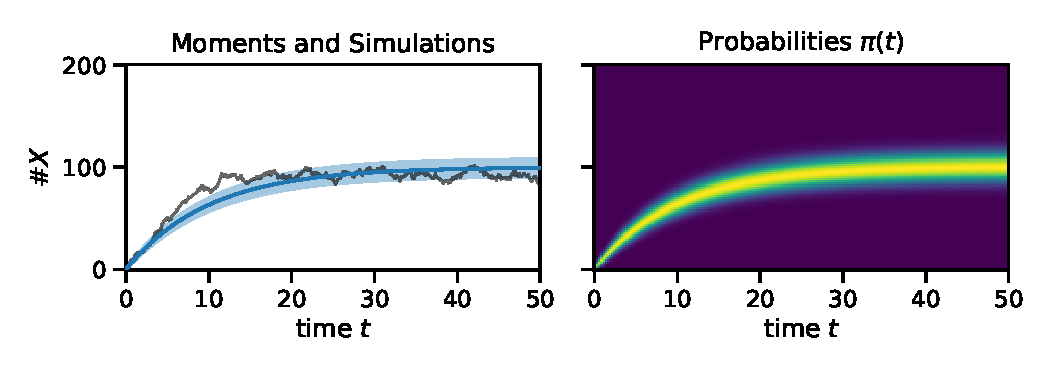
\includegraphics[width=0.9\textwidth]{gfx/momsandprobs.pdf}
	\caption[Moments and probability distribution $\pi(t)$]{\label{fig:momsandprobs}The expected value $\pm$ a standard deviation along with a sampled trajectory (left) and the probability distribution over time (right) of \autoref{model:bd} with $\mu=10$ and $\gamma=0.1$.}
\end{figure}

\subsection{Hybrid Representations}
\begin{itemize}
	\item Equivalent results are obtained by modifying the network to have 1 species per abundancy (basically rule based)
\end{itemize}
\cite{hasenauer2014method,kazeroonian2014modeling,andreychenko2015reconstruction}

\section{Stationary Distribution}\label{sec:stationary_dist}
Assuming
% irreducibility and 
ergodicity  
of the underlying chain, a stationary distribution $\pi_{\infty}$ is an invariant distribution, namely a fixed point of the Kolmogorov forward equation \eqref{eq:forward}.
Let $\pi_{\infty}$ be the vector description of a stationary distribution. It then  satisfies
\begin{equation}\label{eq:stationary}
0=\pi_{\infty}Q\quad
\end{equation}
as a fixed point of the Kolmogorov equation \eqref{eq:forward}.
Furthermore, the solution is constrained, to form a probability distribution, i.e.\ a measure with
unit mass. Thus,
\begin{equation}
1=\sum_{x\in\mathcal{S}}\pi_{\infty}(x)\,.
\end{equation}
Stationary distributions are connected to the \emph{long-run} behavior of an \ac{MPM}~\cite{dayar2011bounding}, as the system's distribution will converge to the (unique)
stationary distribution.
The connection of the stationary distribution to the long-run behavior becomes clear when considering the ergodic theorem. 
For some $A\subseteq\mathcal{S}$,
\begin{equation}\label{eq:ergodic}
    \lim_{T\to\infty}\frac{1}{T}\int_0^T 1_A(X_t)\,dt
    = \sum_{x\in A}\pi_{\infty}(x)\,.
\end{equation}
Thus, the mean occupation time for set $A$ over infinite trajectories is the stationary measure for $A$.
Eq.~\eqref{eq:ergodic} shows that we can assess long-run behavior using the stationary distribution and vice-versa.

\begin{example}
	Returning to the example of \autoref{model:bd} it is obvious that the state-space is irreducible.
Further, we can easily show, that the stationary distribution is Poissonian with rate $\mu/\gamma$:
	\[ \pi_{\infty}(x)=\frac{{(\mu/\gamma)}^{x}\exp(-\mu/\gamma)}{x!}\,.\]
\end{example}


For simplicity, we assume throughout that the state-space is composed of a single communicating class.
Checking ergodicity given a countably infinite number of states is achieved by providing a suitable Foster-Lyapunov function \cite{meyn2012markov}.
Some automated techniques have been proposed for this task \cite{dayar2011bounding,gupta2014scalable,milias2014optimization}.



\subsection{Foster-Lyapunov Bounds}\label{sec:statagg:lyapunov}
It is well-known that for a \ac{CTMC} $X$, ergodicity can be proven by a Foster-Lyapunov
 function $g:\mathcal{S}\to\mathbb{R}$ \cite{meyn1993stability,dayar2011bounding}.
 This is the stochastic analogue of the Lyapunov functions, used to prove convergence of \acp{ODE}.
%The positivity requirement can somewhat be relaxed. The function only needs to be bounded from below since it can be shifted to the positives. In practice this shift can be ignored since it cancels out in the drift \eqref{eq:drift}.
The function $g$ is required to have finite level sets:
\[
	\left|\{x\in\mathcal{S} \mid g(x) < l\}\right|<\infty,\quad \forall l > 0.
\]
Typical choices for $g$ are linear \cite{gupta2014scalable,milias2014optimization} or quadratic \cite{spieler2014numerical}.
Given the $g$, we define its \emph{drift} $d$ as its average infinitesimal change, which is obtained applying the generator $Q$ to $g$.\marginpar{Intuitively, $g$ is interpreted as a vector with the values $f(x_i)_i=f_i$ with the same ordering as in $Q$.}% See also \autoref{sec:moments_bg}.}
\begin{equation}\label{eq:drift}
	d(x) = Qg(x) = \sum_{j=1}^{n_R} \alpha_j(x) (g(x+v_j) -  g(x))
\end{equation}
As such the drift can be interpreted as the expected local tendency of change of a scalar valued function $g$, \marginpar{Note that we end up with \eqref{eq:mom_ode} taking the expectation.}i.e.\ 
\[
	d(x) = \frac{d}{dt}\E{g(X_t)\mid X_t = x}\,.
\]
A Lyapunov function can be used to prove ergodicity of a \ac{CTMC}: If there is a finite subset $C\subset\mathcal{S}$ such that
\begin{align}
	&Qg(x)\leq -1,\; \forall x\in\mathcal{S}\setminus C\,,\label{eq:neg_outside}\\
	&Qg(x)< \infty,\; \forall x\in C\,, \text{ and}\label{eq:pos_inside}\\
	&\lVert x\rVert\to\infty \Rightarrow g(x)\to\infty\,,\;\text{ where }\;\lVert x\rVert=\sum_i x_i\,,\label{eq:lya_normlike}
\end{align}
then the chain is non-explosive and ergodic~\cite{milias2014optimization,tweedie_1975}.
Intuitively, $g(X_t)$ should be a supermartingale outside $C$ and a submartingale inside.
Since the $g$ is norm-like due to \eqref{eq:lya_normlike} this entails that the process
tends towards $C$ when outside, and out of from $C$ when inside.


Given the above requirements
\begin{equation}\label{eq:lyapunov_set}
    \mathcal{C}_{\epsilon_{\ell}} = \left\{ x\in\mathcal{S} \mid
    \frac{\epsilon_{\ell}}{c}d(x) > \epsilon_{\ell} - 1\right\}
\end{equation}
is finite, where 
\[
	\infty> c\geq \sup_{x\in\mathcal{S}} d(x)\,.
\]
In this case, $\mathcal{C}_{\epsilon_{\ell}}$ contains at least $1-\epsilon_{\ell}$ of stationary probability mass for any $\epsilon_{\ell}\in(0,1)$ \cite[Thm.~8]{spieler2014numerical}.
Given that $\mathcal{C}_{\epsilon_{\ell}}$ is finite, the chain is ergodic and
\begin{equation}
    \sum_{x\in\mathcal{C}_{\epsilon_{\ell}}}\pi(x)> 1 - \epsilon_{\ell}
\end{equation}
bounding the stationary probability mass contained within $\mathcal{C}_{\epsilon_{\ell}}$.
\begin{example}
	We return to \autoref{model:bd} and choose $g(x) = x$.
	Then \[ d(x) = \mu - \gamma x\,. \]
	The requirements \eqref{eq:neg_outside}, \eqref{eq:pos_inside},
	and \eqref{eq:lya_normlike} are fulfilled for
	\[ C=\left\{0,\dotsc,\frac{1+\mu}{\gamma} - 1\right\} \]
	and the underlying chain is ergodic. We can further bound the stationary distribution.
	Letting $c=\mu$,
	\[ \frac{\epsilon_{\ell}}{\mu}d(x) = \epsilon_{\ell} - \frac{\epsilon_{\ell}\gamma}{\mu}x \]
	and following \eqref{eq:lyapunov_set} the states
	\[ 0\leq x<\frac{\mu}{\epsilon_{\ell}\gamma}  \]
	have at least $1-\epsilon_{\ell}$ stationary mass.
\end{example}



\section{A Brief Taxonomy of Multimodality}\label{sec:multimodality}
Multimodality is an overloaded term in the context of reaction network models.
Specifically, it can be used to describe the following features.
\begin{description}
	\item[Operational Multimodality]
		This kind of multimodality characterizes the model behavior directly.
		Consider, for example, a gene
		expression model\marginpar{See \autoref{model:gexpr}
		on page~\pageref{model:gexpr} for an example of this.}:
		The gene state is digital, meaning it is either active or inactive.
		Depending on this state a protein is either synthesized or not.
		Therefore the system has distinct \emph{operational modes}
		which dictate its dynamics.
		Non-biological examples can be found in the
		context of broadcasting systems,
		in which the dynamics change discretely due to messages shared between
		agents~\cite{bortolussi2020fluid}.

		Naturally, nearly all models change their dynamics,
		given a change in their state vector.
		In this aspect this distinction is not wholly strict.
		It is mainly intended to indicate distinctive changes in the dynamics.
		In some instances, these can be as obvious as the examples mentioned above.
		In other cases they may not be as obvious:
		Consider an epidemics die-out for example, which is a significant change
		in the operating mode, which is not due to a switch-type reaction.
  \item[Distributional Multimodality]
	  Here the multimodality refers to the stationary distribution $\pi_{\infty}$:
		It has multiple
		\emph{modes}, i.e.\ local maxima. Given an ergodic underlying \ac{CTMC}
		this entails, that the system spends most time in distinct regions of the
		state-space (cf.\ \eqref{eq:ergodic}).
		The \emph{switching} between those distinct region is of interest
		for both, analysis and control, of such models.
\end{description}
While distributional multimodality implies operational multimodality, the reverse
does not hold.

Literature:
\begin{itemize}
	\item \cite{siegal2011emergence}
\end{itemize}

\ctparttext{
	We use moment properties
	to provide bounds on mean first-passage times and
	to improve statistical estimation of different quantities.
%%%%%%  In particular, we use the variance reduction technique
%%%%%%  of \emph{linear control variates} in connection with these moment
%%%%%%  constraints.
}
\part{Moment-Based Methods}\label{pt:moments}
\cleardoublepage%************************************************
\chapter{Bounding Mean First-Passage Times}\label{ch:MFPT}






%\title{Bounding Mean First Passage Times in\\   Population Continuous-Time
%Markov Chains}
%\titlerunning{Bounding Mean First Passage Times in \acp{MPM}}
%\author{Michael Backenk\"ohler${}^{1,2}$, Luca Bortolussi${}^{3,1}$, Verena Wolf${}^{1}$}
%\authorrunning{M.\ Backenk\"ohler et al.}
%\institute{${}^{1}$Saarland University, Germany,\\ ${}^{2}$ Saarbr\"ucken Graduate School of Computer Science,\\
%${}^{3}$University of Trieste, Italy}
%\maketitle
%\begin{abstract}
%  We consider the problem of bounding mean first passage times and reachability probabilities
%  for the class of population continuous-time Markov chains,  which capture stochastic interactions between groups of identical agents.
%  The  quantitative analysis of such models
%  is notoriously difficult since typically neither   state-based numerical
%  approaches nor methods based on stochastic sampling give efficient and accurate results.
%  Here, we propose a novel 
%  approach that leverages techniques from martingale theory and stochastic processes to generate constraints on the statistical moments of first passage time distributions. These constraints induce a semi-definite program that can be used to compute exact bounds on reachability probabilities and mean first passage times without numerically solving the transient probability distribution of the process or sampling from it.
%We showcase the method on some test examples and tailor it to  models exhibiting multimodality, a class of particularly challenging scenarios from biology.
%\keywords{population continuous-time Markov chains \and semi-definite programming
%  \and exit time distribution \and reachability probability \and Markov population models}
%\end{abstract}

%\section{Introduction}
For the quantitative analysis of \acp{CTMC}, many   approaches have been
developed, where properties of interest are often expressed in terms of temporal logics such as
\acs{CSL}~\parencite{aziz1996verifying,baier2000model,baier2003model,spieler2014model},
\acs{MTL}~\parencite{chen2011time},
and specifications for timed-automata~\parencite{chen2009quantitative,mikeev2013fly}.
In addition, there exist
efficient software
tools~\parencite{hinton2006prism,kwiatkowska2011prism,dehnert2017storm}
that can be used to analyze and verify system properties.
The computation of reachability probabilities is a central problem in this context.

Popular exact methods for \acp{CTMC} rely on numerical approaches that explicitly consider each system state individually.
A major problem is that these methods cannot scale in the context of population
models with large copy numbers of agents.
A popular alternative to tackle this problem is statistical model checking,
which is based on stochastic simulation~\parencite{david2015statistical}.
For \acp{MPM}   arising in the context of chemical reaction networks, trajectories of the process are
usually generated using the \ac{SSA}~\parencite{gillespie1977exact}.
However, since the number of possible interactions grows with the number of
agents, stochastic simulations of \acp{MPM} are  time-consuming. Moreover, they are
subject to inherent statistical uncertainty and give only statistically estimated bounds.

As an alternative, recent work concentrates on numerical methods that
approximate the statistical moments of the system without the need to
compute the probability of each state.
For groups of identically behaving agents, it is possible to derive systems of
differential equations
for the evolution of the statistical population
moments~\parencite{bogomolov2015adaptive,schnoerr2017survey,bortolussi2013model,engblom2006computing,schnoerr2015,gast2019}.
However, as the system of exact moment equations is infinite-dimensional, approximation
schemes typically rely on certain assumptions about the
underlying probability distribution to truncate it.\turnto{sec:fsp}
For example, one might employ a ``low dispersion closure'' which assumes that
higher-order moments are the same as those of a normal
distribution~\parencite{hespanha2008moment}. %\vw{Hespanha macht doch lognormal?}\todo{in dem papier macht er eine survey f\"ur sein tool}
Such approximations are, by nature, ad-hoc and do not come with
any guarantees.


Moment-based methods often scale well   in terms of population sizes. However,
it is not possible to control the effects of the introduced approximations, which in some
cases can lead to large errors~\parencite{schnoerr2015}.
This issue reverberates
on the application of these methods to  compute reachability
probabilities and \aclp{MFPT}~\parencite{hayden2012fluid,bortolussi2013model,bortolussi2014stochastic}.
Moreover, they can suffer from numerical instabilities, in particular, when the
maximum order of the considered moments has to be increased to more
appropriately describe the underlying distribution. %, a fact impacting their
%scalability.

Here, we put forward a method based solely on moments that gives \emph{exact bounds}  for \acfp{MFPT} and reachability probabilities in \acp{MPM}\@.
For a set of states $B$ and a time-horizon $T$, the \ac{FPT}
\[
	\tau = \inf\{t\geq 0\mid \vec X_t \in B\} \land T\,.
\]
This mean of this stopping time $\E{\tau}$, i.e.\ the \acl{MFPT}, directly characterizes the probability of reaching set $B$
within $T$ time units. Thus, safe upper and lower bounds on \acp{MFPT} can constitute a core component for the verification of properties in \acp{MPM}\@.
Our approach extends recent work on moment
bounds~\parencite{sakurai2017convex,dowdy2018dynamic} and it is based on a martingale formulation of the stopped process that we
derive from the exact moment equations. From this formalization, we deduce a set
of linear moment constraints from which we derive
upper and lower moment bounds using \acf{SDP}\@. Monotone
sequences of both upper and lower bounds
can be obtained by increasing the order of the relaxation. Crucially, no
closure approximations are introduced.
Therefore the bounds are exact up to the numerical accuracy of the \ac{SDP} solver.


To experimentally validate our method in terms of accuracy and feasibility, we run some tests on examples from biology, leveraging an existing \ac{SDP} solver and obtaining encouraging results. 
Comparing with other moment-based methods, our approach is not based on approximations due to closure schemes, thus providing guarantees on the bounds   up to the numerical accuracy of the computations. However, similarly to other moment-based methods, we also found the insurgence of numerical instabilities because moments of higher order tend to span over many orders of magnitude. We ameliorate this problem by considering scaling strategies that reduce such variability. 
We also extend our approach to deal with \acp{MPM} exhibiting strong multimodal behavior, due to the presence of populations having low copy numbers. This extension exploits some ideas from hybrid moment closures~\parencite{kazeroonian2014modeling}. 


% For our numerical investigations, we concentrate  and find encouraging
% results already for a small number of moments.
% For instance, in one of our case studies  $100,000$ \ac{SSA} runs are necessary to
% achieve a relative   width of 0.9\% for the \ac{MFPT} confidence interval.
% The \ac{SDP} solver, however, returns a guaranteed interval with 
% a relative width of 0.3\%.\\



\noindent
In summary, this chapter presents the following novel contributions:
\begin{itemize}
	\item the derivation of moment constraints, based on a martingale formulation, for bounding \aclp{MFPT}
      and reachability probabilities using a convex programming scheme;
      %using a martingale formulation;
    \item the extension of this scheme using hybrid moment conditions to systems
      exhibiting multimodal behavior;
    % \item a scaling strategy for improved robustness during optimization
\end{itemize}

\section{Related Work}\label{sec:mfpt:related}
\paragraph{Truncations and Analytic Solutions} Considerable effort has been directed at the analysis of \acl{FPT}
distributions in \acp{MPM}\@. Most works can either focus on an explicit state-space
analysis~\parencite{barzel2008calculation,munsky2009specificity,kuntz2019exit,kuntz2021approximations}
or employ approximation techniques for which, in general, no error bounds can be
given~\parencite{schnoerr2017efficient,hayden2012fluid,bortolussi2014stochastic}.
For some model classes such as kinetic proofreading, analytic solutions are
possible~\parencite{munsky2009specificity,bel2009simplicity,iyer2016first}.

\citet{barzel2008calculation} propose a recursive scheme that consists of one equation for
each state, expressing the average time the system needs to transition from that
state to the target state.
\citet{kuntz2021approximations} propose to employ moment bounds in a
linear programming approach to compute exit time distribution using state-space
truncation schemes. In \citet{kuntz2019exit} the authors propose a finite state-space
projection scheme to bound \acl{FPT} distributions

\paragraph{Moments Approximations} In \citet{hayden2012fluid}, the authors
use moment closure approximations and
Chebychev's inequality to gain an understanding of \acl{FPT} dynamics.
\citet{schnoerr2017efficient} also employ a moment closure approximation
and further approximate threshold functions to derive an approximate \acl{FPT}
distribution.
\citet{bortolussi2014stochastic} use a mean-field approximation
which is required to reach the target region.

\paragraph{Moment Bounds using Optimization} Recently, several groups independently suggested the use of semi-definite
optimization for the computation of moment bounds for the limiting
distribution~\parencite{ghusinga2017exact,dowdy2018bounds,kuntz2017rigorous,sakurai2017convex}.
In this approach, the differential equations describing the moment dynamics are
set to zero and form linear constraints~\parencite{backenkohler2018moment}. Alongside, semi-definite constraints can
be placed on the \emph{moment matrices}. These give a semi-definite program
that can be solved efficiently.

This approach has been extended to the transient
case~\parencite{dowdy2018dynamic,sakurai2019bounding}.
The approach is similar in both works and is a cornerstone of the \ac{MFPT} analysis
presented here.
They differ mainly by the fact that \citet{sakurai2019bounding} apply a polynomial
time-weighting, while \citet{dowdy2018dynamic} use an
exponential one. We adopt the former approach because it
can be naturally adapted to the description of densities over time.
The resulting forms can also be adapted to statistical estimation
problems~\parencite{backenkohler2019control}.

Semi-definite programming has been applied to a wide range of problems,
including stochastic processes in the context of financial
mathematics~\parencite{lasserre2006pricing,kashima2009polynomial}.
For good introductions and overviews of application areas, we refer
the reader to \citet{parrilo2003semidefinite} and, more recently,
\citet{lasserre2010moments}.

\paragraph{Bounding MFTPs using Optimization}
Particularly relevant for this work is the application of convex optimization to
\ac{FPT}\@.
\citet{helmes2001computing} formulated a linear program using the
%basic adjoint equation and
Hausdorff moment conditions \parencite{hausdorff} to bound moments of the
\ac{FPT} distribution in Markovian processes.
Semi-definite optimization has been successfully applied in financial
mathematics by \citet{kashima2009polynomial}, as well as
\citet{lasserre2006pricing} to bound prices of exotic options.
%Here, the approach by Lasserre is adapted to \acp{MPM}.

\section{Preliminaries}\label{sec:mfpt:bg}



In this work, we are interested in \acfp{FPT} of such processes.
That is the time, the process first enters a set of target states
$B\subseteq \mathcal{S}$. Naturally, the analysis of \acp{FPT} is
equivalent
to the analysis of times at which the process exits the complement $\mathcal{S}\setminus B$.
More formally, the \acl{FPT} $\tau$ for
some target set $B$ is defined as the random variable
\begin{equation}\label{eq:fpt_def}
    \tau = \inf\{t\geq 0\mid \vec X_t \in B\}\,.
\end{equation}


In this example, we are interested in the time at which the number of type $M$ agents
exceed some threshold $H$.
With the framework presented in the sequel, one can bound the expected value
of this time using semi-definite programming.
Further, it is possible to impose a time-horizon $T$, and find bounds
on the probability of $ X_t^{(M)}\geq H$ for some $0\leq t\leq T$.
The employed framework is centered around semi-definite relaxations
of the \ac{GMP}~\parencite{lasserre2010moments}.
These require linear constraints on the moments of measures.
In the following section, we derive such constraints.

\section{Martingale Formulation}\label{sec:mfpt:moments}
Next, we will discuss the ordinary differential equations for the evolution of the statistical moments of
the process.
The moments over the state-space are then used to derive temporal moments, i.e.\ moments
of measures over both the state-space and the time.
This extended description results in a process with the martingale property.
This property can be used to formulate linear constraints on the temporal moments
and, as a special case, the mean first-passage time.
In combination with semi-definite properties of moment matrices, we can formulate
mathematical programs that yield upper and lower bounds on \aclp{MFPT}\@.


Let $f$ be a polynomial function, $t\ge0$.
Using the \ac{CME} \eqref{eq:cme}\turnto{eq:cme}, we can derive \acp{ODE}
describing the dynamics of $\expSym(f(\vec{X}_t))$~\parencite{engblom2006computing}.
Specifically,\graffito{More details on the derivation of the moment \acp{ODE} is given in \autoref{sec:moments_bg}.}
\begin{equation}\label{eq:mfpt:mom_ode}
    \frac{d}{dt}\E{f(\vec X_t)} = \sum_{j=1}^{n_R}\E{\left(f({\vec X_t +
    \vec{v_j}}) - f(\vec X_t)\right)\alpha_j(\vec X_t)}\,.
\end{equation}

\begin{example}
Let us consider \autoref{model:dim} and agent type $M$ as an example.
Further, let $X_t=X_t^{(M)}$
for ease of exposition.
When choosing $f(X_t)=X_t^m$, $m=1$ and   $m=2$
we obtain two differential equations describing
the change of the first two moments of species $M$,
$\E{X_t}$ and $\E{X_t^2}$, respectively.
\begin{equation}\label{eq:dim_exp_ode}
	\begin{split}
    \frac{d}{dt}\E{{X}_t} &= \lambda\E{{X}_t^0} -
    2{\delta}\left(\E{{X}_t^2}-\E{{X}_t}\right)\\
    \frac{d}{dt}\E{{X}_t^2} &= \lambda(2\E{{X}_t} + 1)\\
		&\quad- 4\delta\left(\E{{X}_t^3} -
    2\E{{X}_t^2} + \E{{X}_t}\right)\,.
	\end{split}
\end{equation}
Fixing initial moments, the \ac{ODE} system describes the moments over time exactly.
However, these \acp{ODE} cannot be integrated because the system is not closed.
The right-hand side for moment $\E{X_t^m}$ always contains $E(X_t^{m+1})$.
\end{example}
To solve the \ac{IVP},
one typically resorts to ad-hoc approximations of the highest order moments
to close the system.
Here we do \emph{not} need such approximations
because we do not numerically integrate the moment equations.
Instead we adopt an approach \parencite{dowdy2018dynamic,sakurai2019bounding} that extends
the description of state-space moments to a temporal one.

This is achieved by the introduction of a time-dependent polynomial $w(t)$ that is multiplied to
\eqref{eq:mfpt:mom_ode}.
An integration by parts on $[0, T]$ yields~\parencite{dowdy2018dynamic,sakurai2019bounding}
\begin{multline}\label{eq:exp_constraint}
        w(T)\E{f(X_{T})}
        - w(t_0)\E{f(X_{t_0})}
	- \int_{t_0}^{T}\frac{dw(t)}{dt}\E{f(X_t)}\,dt\\
        =\sum_{j=1}^{n_R}\int_{t_0}^{T}w(t)
        \E{\left(f{(X_t + v_j)} - f(X_t)\right)\alpha_j(X_t)}\,dt\,.
\end{multline}
Starting from this equation, it is possible to derive a martingale process,
i.e.\ a process that has an expected value equal to \num{0}, regardless of time.


We now want to interchange the order of integration and the summation due to the expected value.
To this end, we have to assume the absolute convergence of the integrals.
On finite time intervals $[0,T]$ this holds because $w$
is polynomial and we assumed finite moments for all $t\geq 0$.
Interchanging the  summation  and integral of a monomial
${\vec{x}}^{\vec{m}}$, i.e.\ pulling all expectation operators outside
\begin{align*}
	& \;\quad\int_{0}^Tg(t)\E{\vec X_t^{\vec m}}\,dt\\
	& =\int_{0}^T\sum_{x\in\mathcal{S}}g(t)\Pr(X_s=x)x^m\,dt\\
	& =\int_{0}^T\int_{\Omega} g(t) {X_s(\omega)}^m\,dP(\omega)\,dt\\
	& =\int_{\Omega}\int_{0}^T g(t) {X_s(\omega)}^m\,dt\,dP(\omega)\\
	& =\E{\int_{0}^Tg(t){\vec X}_t^{\vec m}\,dt}.
\end{align*}
Hence, we are able to to pull out the expectation operator in~\eqref{eq:exp_constraint}.
\begin{equation}\label{eq:e_exp_constraint}
\begin{split}
    0=&\,w(T)\E{f(\vec X_T)} - w(0)\E{f(\vec X_{0})} -
    \E{\int_{0}^T\frac{dw(t)}{dt}f(\vec X_t)\,dt}\\
    &-\sum_{j=1}^{n_R}\E{\int_{0}^Tw(t)
         (f(\vec X_t+\vec v_j) - f(\vec X_t))\alpha_j(\vec X_t)\,dt}\,,
         \end{split}
\end{equation}
This gives us the expected value of a time-dependent function of the original process.
The function can be viewed as a stochastic process of its own where the
time-horizon $T$ is the index variable. A key property
of this process is also illustrated by \eqref{eq:e_exp_constraint}: The process'
expected value remains zero, regardless of the choice of $T$.
This martingale property is particularly useful because it can be used
to formulate linear constraints on stopping times of the process.
Explicitly, we can define this process $\{Z_T\}_{T\geq 0}$ parameterized by
the time-weighting $w$ and polynomial $f$.
\begin{equation}\label{eq:martingale}
\begin{split}
    Z_T\coloneqq&\,w(T)f(\vec X_T) - w(0)f(\vec X_{0}) -
    \int_{0}^T\frac{dw(t)}{dt}f(\vec X_t)\,dt\\
    &-\sum_{j=1}^{n_R}\int_{0}^Tw(t)
         (f(\vec X_t+\vec v_j) - f(\vec X_t))\alpha_j(\vec X_t)\,dt\,.
         \end{split}
\end{equation}
A useful choice for $f$ and $w$ are monomials.
When choosing $w(t)=t^k$
\marginpar{In \autoref{ch:cvinsrns} we use an exponential weighting.}
with $k\in\mathbb N$ and $f(\vec X)={\vec X}^{\vec m}$
the process takes the form
\begin{equation}\label{eq:basic_poly_martingale_app}
Z_T^{(\vec m, k)}=
         T^k \vec X_T^{\vec m}
        - 0^k \vec X_{0}^{\vec m}
        % - k \int_0^T t^{k-1} \vec X_t^{\vec m}\,dt
        + \sum_{i}c_i\int_0^T t^{k_i} \vec X_t^{\vec m_i}\,dt
\end{equation}
where   $(\vec m_i)_i$, $(k_i)_i$, and $(c_i)_i$ are finite sequences resulting
from the substitution
of $f$ and $w$
and expansion of~\eqref{eq:martingale}.


When choosing $w(t)=t^k$ with $k\in\mathbb N$ and $f(\vec X)={\vec X}^{\vec m}$
this process takes the form
\begin{equation}\label{eq:basic_poly_martingale}
Z_T^{(\vec m, k)}=
         T^k \vec X_T^{\vec m}
        - 0^k \vec X_{0}^{\vec m}
        % - k \int_0^T t^{k-1} \vec X_t^{\vec m}\,dt
        + \sum_{i}c_i\int_0^T t^{k_i} \vec X_t^{\vec m_i}\,dt
\end{equation}
where   $(\vec m_i)_i$, $(k_i)_i$, and $(c_i)_i$ are finite sequences resulting
from the substitution
of $f$ and $w$.
 This choice allows to naturally
characterize the behavior in time and state-space as moments, because
the expected value of \eqref{eq:basic_poly_martingale} then becomes a linear form
of moments.
We will use these as constraints in the semi-definite program used to bound \acp{MFPT}.

% \todo{re-state the above example here again?}\luca{good idea}
\begin{example}
If we apply this to our previous example (cf.\ \eqref{eq:dim_exp_ode}), letting $m=1$ %\vw{same example has $\vec m=(1,0)$ above }
and $k=1$ we obtain the following process for \autoref{model:dim}.
\begin{multline*}
    Z_T^{(1,1)} = TX_T - \int_0^T X_t\,dt
	- \lambda \int_0^T t\,dt\\ - 2\delta
    \int_0^T t X_t\,dt +
    2{\delta}\int_0^TtX_t^2\,dt,
\end{multline*}
where the sequences according to \eqref{eq:basic_poly_martingale} are $(m_i)_i=(1,0,1,2)$, $(k_i)_i=(0,1,1,1)$,
and $(c_i)_i=(-1,-\lambda, -2\delta,2\delta)$.
\end{example}
%\section{Bounds for Mean First-Passage Times}\label{sec:mfpt:mfpt_bounds}
We now turn to the analysis of first passage times within some time-bound
$T>0$. Given some subset of the state-space
$B\subseteq \mathcal{S}$ the first passage time is given by the continuous random variable 
\[
	\tau = \inf\{t\geq 0\mid \vec X_t \in B\} \land T
\]
where $a \land b \coloneqq \min\{a, b\}$.
For this chapter, we only look at threshold hitting times,
i.e.\ we set a threshold $H$ for species $S$ and thus 
\[
	B=\{\vec{x}\mid x^{(S)}\geq H\}\,.
\]
Note, that this framework
allows for a more general class of target sets, which are discussed in
\autoref{subsec:mfpt:multidim}.
In the sequel, we will use $\tau$ as a stopping time in our martingale
formulation and consider
$Z_\tau^{(\vec m, k)}$ instead of $Z_T^{(\vec m, k)}$.
Since~\eqref{eq:basic_poly_martingale} defines a martingale, $Z_{\tau}^{(\vec m, k)}$
remains a martingale by
Doob's optional sampling theorem~\parencite{gihmantheory}. In particular, this
implies that 
\begin{equation}\label{eq:zero_constraint}
	\expSym(Z_{\tau}^{(\vec m, k)})=0
\end{equation}
for all moment orders $m$ and
degrees $k$ in the weighting function $w(t)$.

\section{Linear Model Constraints}
To simplify our presentation, we fix an initial state $\vec x_0$, i.e.\ $P(\vec X_0=\vec x_0)=1$.
Expanding \eqref{eq:zero_constraint} using
\eqref{eq:basic_poly_martingale} for $Z_{\tau}^{(\vec m, k)}$
yields the following linear constraint on expected values.
\begin{equation}\label{eq:constraint}
    0 = \,\E{{\tau}^k\vec X_{\tau}^{\vec m}}
        - 0^k\vec x_0^{\vec m}
        % - k \E{\int_{0}^{\tau} t^{k-1} \vec X_t^m\,dt}
        + \sum_{i}c_i\E{\int_{0}^{\tau} t^{k_i} \vec X_t^{\vec m_i}\,dt}\,,
\end{equation}
where $0^0=1$.
Hence, we have established a relationship between the process dynamics
up to the hitting time via expected values of the time-integrals and the final process state at
the hitting time via $\E{\tau^k {X}_{\tau}^{{m}}}$.

For the ease of exposition, we now turn to the analysis of first passage times in
one-dimensional processes w.r.t.\ an upper threshold $H$. In particular,
we will consider  moments $\expSym(X^m)$, $m=0,1,2,\dots,$ of a one-dimensional process.
The   approach proposed in the sequel, however,
can be extended to multi-dimensional processes and more complex target sets $B$.

\begin{example}
	Consider again \autoref{model:dim} and assume that we are interested in the
time at which species $M$ exceeds  threshold $H$ while fixing the considered time-horizon to
$T=4$. That is, we are interested in the stopping time
\[
	\tau=\inf\{t\geq 0\mid X_t\geq 10\}\land 4\,.
\]
Since the abundance of $D$ does not influence $M$, we can ignore
species $D$ and treat the process as one-dimensional.
\autoref{fig:decomposition} shows three example trajectories:
Two reach an upper threshold $H=10$, while one reaches the final time-horizon $T=4$.
The figure also illustrates another aspect present in \eqref{eq:constraint}.
It gives a connection between the terminal distribution, i.e. the distribution of $X_{\tau}$,
and the dynamic behavior up to $\tau$.
The statistics at $\tau$ are described by a distribution whose %\luca{what are nu 1 and 2? they have not introduced before}
moments are represented by the $E(\tau^k{\vec{X}_{\tau}}^{\vec{m}})$ term in \eqref{eq:constraint}.
This distribution corresponding two moments encompasses both cases of how
$\tau$ can be reached. In the first case threshold $H$ is reached and the second case the process reaches the time-horizon $T$.
In the following we will define the interplay between these measures more formally.
\begin{figure}[htb]
    \centering
    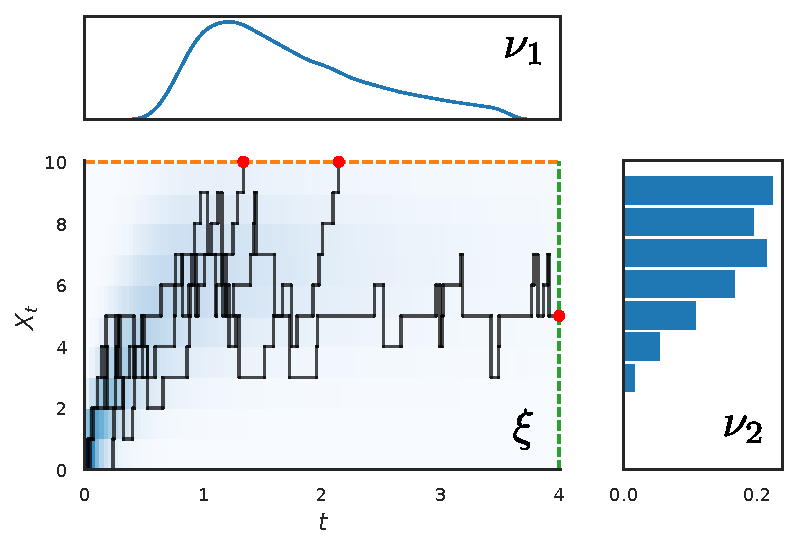
\includegraphics[scale=.8]{gfx/decomp1.pdf}
	\caption[Occupation measure $\xi$ and
	exit location probability measures $\nu_1$ and $\nu_2$]{The relationship between the occupation measure $\xi$ and the
    exit location probability measures $\nu_1$ and $\nu_2$. The shaded area indicates
    the structure of the occupation measure. Three example trajectories are
    additionally plotted with
	their exit location highlighted. The plots are based on \num{10000} sample trajectories.}
    \label{fig:decomposition}
\end{figure}
\end{example}


Eq.~\eqref{eq:constraint}  describes a relationship between
two measures~\parencite[][Chapter~9.2]{lasserre2010moments}:
\begin{description}
\item[Expected Occupation Measure] $\xi$ describes the expected residence time inside a subset of the state-space and time. As such it is supported on $[0,H]\times [0,T]$:
\begin{equation}\label{eq:ex_occ_measure}
    \xi(A\times C) \coloneqq \E{\int_{[0,\tau]\cap {C}}{1}_{\in A}(X_t)\,dt},
\end{equation}
\item [Exit Location Probability] $\nu$ gives the state probability associated with the stopping time $\tau$. Therefore it is supported on $(\{H\}\times[0,T]) \cup
([0,H]\times\{T\})$:
% \todo{this can also be dropped, ie.\ we don't set a time-horizon. should be fine if passage time moments are finite (also
% in the relaxation)}
\begin{equation}\label{eq:exit_loc_measure}
    \nu(A\times C)\coloneqq \Pr((X_{\tau},\tau)\in A\times C),
\end{equation}
\end{description}
where $A\times C$ is a measurable set, i.e.\ $A$ and $C$ are elements of the Borel $\sigma$-algebras on $[0,H]$ and $[0,T]$, respectively.

Using \autoref{fig:decomposition}, one can gain an intuition for these two measures.
The expected occupation measure is shaded in blue.
As the name implies $\xi(A\times C)$ tells us how much time  the process spends
in $A$ up
to $\tau$ restricting to the time instants belonging to $C$.
In particular, $\xi([0,H]\times [0,T])=\E{\tau}$.
The exit location probability $\nu$, while being a two-dimensional distribution, can be viewed as a composition of a density describing the time at which the process reaches $H$ (if it does) and a probability mass function on the states of the process if the time-horizon is reached without exceeding $H$.
We partition the measure $\nu$ into $\nu_1$ and $\nu_2$ by conditioning on $\tau=T$.
Thus, 
\[
	\nu_1(C)\coloneqq\Pr(\tau\in C, \tau<T)
\]
and
\[
	\nu_2(A)\coloneqq\Pr(X_T\in A, \tau=T)
\]
and hence $\nu(A\times C)=\nu_1(C)+\nu_2(A)$.
To refer to the moments of these measures, we define \emph{partial moments}
\[
    \E{g({X}); f({Y}) = y}\coloneqq
    \E{g({X})\mid f({Y})=y}\Pr(f({Y})=y)\,,
    \]
for some polynomial $g$ and some indicator function $f$. Then
\[
	\E{\tau^k X_{\tau}^m}=T^k\E{X_{\tau}^m;\tau=T} + H^m\E{{\tau}^k;\tau < T, X_{\tau}=H}\,.
\]
% The partial expectations in terms of $\nu_1$, $\nu_2$
% \[
% \E{X_{\tau}^m;\tau=T} + \E{{\tau}^k;\tau < T, X_{\tau}=H}
% \]
Therefore the linear moment constraints are
\begin{multline}\label{eq:model_constraints}
 	0 = T^k\E{X_{\tau}^m;\tau=T} + H^m\E{{\tau}^k;\tau < T, X_{\tau}=H}\\
 	- 0^kx_0^{m}
 	% - k \E{\int_{0}^{\tau} t^{k-1} \vec X_t^m\,dt}
 	+ \sum_{i}c_i\E{\int_{0}^{\tau} t^{k_i}X_t^{m_i}\,dt}\,.
\end{multline}
% \begin{multline*}
% 	0 = \,&T^k\E{X_{\tau}^m;\tau=T} + H^m\E{{\tau}^k;\tau < T, X_{\tau}=H}\\
% 	- 0^kx_0^{m}
% 	% - k \E{\int_{0}^{\tau} t^{k-1} \vec X_t^m\,dt}
% 	+ \sum_{i}c_i\E{\int_{0}^{\tau} t^{k_i}X_t^{m_i}\,dt}\,.
% \end{multline*}
Next, we consider infinite sequences of partial moments 
 $\vec{y}_1=(y_{1k})_{k\in\mathbb{N}}$, $\vec{y}_2=(y_{2m})_{m\in\mathbb{N}}$, and $\vec{z}=(z_{mk})_{(m,k)^{\T}\in\mathbb{N}^2}$
 of $\nu_1$, $\nu_2$, and $\xi$, respectively.
 In particular,
\begin{align*}
	y_{1k} &\coloneqq \E{{\tau}^k;\tau < T}\,,\\
	y_{2m} &\coloneqq\E{X_{\tau}^m;\tau=T}\,,
\intertext{and}
	z_{km} &\coloneqq\E{\int_0^{\tau}t^k X_t^m\,dt}\,.
\end{align*}

\section{Objective}
Given the above measures and their corresponding moments, we can
now identify the moments we are particularly interested in.
We formulate an optimization problem with variables corresponding 
to the moments defined above.
The \ac{MFPT} is exactly the zeroth moment of $\xi$,
\[
	z_{00}=\E{\int_0^{\tau}1_{\leq H}(X_t)\,dt} = \E{\tau}\,.
\]
Therefore $z_{00}$ corresponds to the objective of the optimization problem
that gives bounds for the \ac{MFPT}.
Furthermore, we can easily change the objective to the  
zeroth moment of $\nu_1$,
\[
	y_{10} = \E{\tau^0;\tau<T}=\Pr(\tau < T)\,.
\]
This moment is the probability of reaching
threshold $H$ before reaching time-horizon $T$. Since the target set can be more complex, this formulation can be used to perform model checking on a
wide variety of properties.

Moreover, it is possible to formulate objectives not directly corresponding to
a raw moment such as the variance~\parencite{sakurai2019bounding,dowdy2018bounds}.

\section{Linear Hausdorff Constraints}
Before discussing the semi-definite constraints which we will use for the remainder of this study, we will briefly discuss the Hausdorff moment constraints.
These constraints offer linear constraints on moments of bounded measures.
The Hausdorff moment problem is the question whether an infinite sequence $(m_0, m_1, \dotsc)$ is a sequence of moments
\[
	m_k = \int_{0}^{1} x^k\,d\mu(x), \quad \forall k\in\mathbb{N}
\]
for some Borel-measure supported on the unit interval $[0,1]$.

\citet{hausdorff} came up with a necessary condition that
\marginpar{See also \citet{feller} for additional details.}
\begin{equation}\label{eq:hausdorff}
    \int_0^1 x^\ell(1-x)^k\,d\mu(x) \geq 0, \quad \forall \ell, k\in\mathbb{N}\,.
\end{equation}
The validity of this condition is easy to see since
\begin{equation}\label{eq:hausdorff_integrand}
	x^\ell(1-x)^k\geq 0, \quad \forall x\in[0,1]\,.
\end{equation}
Expanding this term yields a polynomial, which --~by integration~-- provides a linear constraint on the moments.
This moment condition has been used by \citet{helmes2001computing} to bound \acp{MFPT} in a variety of stochastic processes.
In \citet{helmes2008geometrical} the authors provide an extension taking into account the geometry of the Hausdorff polytope.
With this extension the method was competitive with the \ac{SDP} approach on their selection of case studies.
Since these conditions are linear in the moments they can solve linear programs instead of the semi-definite programs shown below.

\begin{example}
	Let $\ell = 2$, $k=2$. Then the \eqref{eq:hausdorff} becomes
	\[
		\int_0^1 x (1 - x)^2 \,d\mu(x) =
		m_2 - 2 m_3 + m_4 \geq 0
	\]
	constraining the moments on $[0,1]$.
\end{example}

Since the Hausdorff moment problem is defined on $[0,1]$, we need to adjust accordingly.
Let the interval be $[0,H]$, $H>0$ then we can simply change the variables.
That means considering $y=x/H$ instead of $x$.
Equivalently, we can apply this rescaling in \eqref{eq:hausdorff} such that
\begin{equation}\label{eq:hausdorff_scaled}
	\int_0^H x^\ell(H-x)^k\,d\mu(x) \geq 0, \quad \forall \ell, k\in\mathbb{N}
\end{equation}
remains a valid constraint on $[0,H]$.

Generalizing \eqref{eq:hausdorff} to multiple dimensions can be done by simply multiplying terms
for each dimension in a similar manner.
For $n$ dimensions
\begin{equation*}
	\int_{{[0,1]}^n}\prod_{i = 0}^n x_i^{\ell_i}{(1-x_i)}^{k_i}\,d\mu{(\vec{x}})\geq 0
\end{equation*}
for all $\ell_i, k_i\in\mathbb{N}$ and $i\in \{0,\dotsc, n\}$.
\marginpar{We treat the time horizon $T$ exactly the same as the other bounds $H_i$ here.}
With arbitrary positive upper bounds $H_1, H_2, \dotsc, H_n$ this becomes
\begin{equation}\label{eq:hausdorff_constraint}
    \int_{\bigtimes_{i=1}^n[0,H_i]}\prod_{i = 0}^n x_i^{\ell_i}{(H_i-x_i)}^{k_i}\,d\mu{(\vec{x}})\geq 0
\end{equation}
This equation can simply be expanded using the multi-binomial theorem. % Taken from Wikipedia : https://en.wikipedia.org/wiki/Binomial_theorem#Multi-binomial_theorem
This is just a vector version of the regular binomial theorem
That is, given $n$-dimensional vectors $k$, $x$, and $y$
\marginpar{We use multi-index notation here.}
\[
    (y+x)^{k} =
    \sum_{j\leq k}
    \binom{k}{j} y^{j}x^{k-j}\,.
\]
% In multi-index notation
% \[
%     (y + x)^k = \sum_{\nu\leq k} \binom{k}{\nu} y^{\nu}x^{k-\nu}\,.
% \]
Thus, \eqref{eq:hausdorff_constraint} becomes the linear moment constraint
\marginpar{We can interchange the integrals since all measures have finite support and mass.}
\begin{equation}\label{eq:hausdorff_appl}
    %\sum_{j_1=0}^{k_1}\dotsm\sum_{j_n=0}^{k_n} 
    \sum_{j\leq k}
    %\left(\prod_{i=1}^{n}\binom{k_i}{j_i}
    \binom{k}{j}
    %H_i^{j_i}(-1)^{k_i-j_i}
    H^j (-1)^{k-j}
    %\right)\\
    %\int_{\bigtimes_{i=1}^n[0,H_i]}
    \int
    x^{k-j+\ell} \,d\mu(x)\geq 0\,.
\end{equation}

\subsection{A Linear Program}
Combining the model constraints \eqref{eq:model_constraints} and the linear Hausdorff-type constraints \eqref{eq:hausdorff_appl} for both expected occupation and the exit location measure yields a linear program.
\begin{equation}\label{eq:lp_for_fpt}
    \begin{split}
	    \text{min} / \text{max} \hspace{1em}&  z_{00}^{\prime} \\
        \text{such that}\hspace{1em} & \text{for all measures and bounds}\\
        &\qquad\eqref{eq:hausdorff_appl}\text{ holds }\forall m, k,\\
        & 0= y_{1k}' H^m -  y_{2m}'T^k - 0^k x_0^m \\
	    &\qquad\quad+\sum_i c_i  z_{k_i m_i}', \quad\forall m, k\,.
    \end{split}
\end{equation}
Using a framework such as \acsfont{CVXPY}, this convex program can easily be coded and solved using various state-of-the-art solvers.

\section{Semi-Definite Constraints}
The linear constraints alone are not sufficient to identify moment bounds.
We further leverage the fact that a necessary condition for a positive measure that the \emph{moment matrices}
are positive semi-definite.
A matrix $M\in\mathbb{R}^{n\times n}$ is positive semi-definite, denoted by  $M\succeq 0$ if and only if
\[
	{\vec v}^T M{\vec v} \geq 0\quad \forall \vec v\in\mathbb{R}^n\,.
\]
\begin{example}
As an example, let us consider a one-dimensional random variable $Z$
with moment sequence $\vec z$.
For  moment order $r$,
the entries of the $(r+1)\times (r+1)$ moment matrix $M_r(\vec x)$ are given by
the raw moments.
In particular, 
\[ 
	(M_r({\vec{z}}))_{ij}=z_{i+j-2}=\E{Z^{i+j-2}}
\]
for
$i,j\in\mathbb{N}_r$ where $\mathbb{N}_r=\{0,1,\dots,r\}$ and the maximum order in the matrix is $2r$.
For instance,
\begin{equation}
\label{eq:m1_dim}
    M_1(\vec x) =
    \begin{bmatrix}
    x_0 & x_1 \\
    x_1 & x_2
    \end{bmatrix}
\end{equation}
needs to be positive semi-definite. By Sylvester's criterion this means $\det
M_1\geq 0$ and $x_0\geq 0$.
We can easily see that in this case this entails
	\[
\det M_1=x_0x_2 - x_1^2=\E{X^2}-\E{X}^2
=\Var({X})
\geq 0\,.
\]
This restriction is natural since the variance cannot be negative.
\end{example}
% Even though the measures $\nu_1$, $\nu_2$, and $\xi$ are not probability measures
% this restriction remains valid for them. Either they can be normalized to
% form a probability measure, or if their mass is zero % we don't care...
The restriction of the non-negative variance we saw in the example generalizes
to moment matrices in form of a positive semi-definite constraint \parencite{parrilo2003semidefinite}.\graffito{This constraint is valid for general positive measures --- even if they do not model probabilities.}
This gives us the following restrictions on the moment matrices.
\begin{equation}\label{eq:sd_constraints}
M_r(\vec{z})\succeq 0, \quad M_r(\vec{y_1})\succeq 0,\quad\text{and}\quad M_r(\vec{y_2})\succeq 0
\end{equation}
for arbitrary orders $r$, providing a first tranche of moment constraints.

Furthermore, we need to enforce the restriction of the measures $\xi$, $\nu_1$, and $\nu_2$
to their supports.
This can be done, by defining non-negative polynomials
on the intended support of the measure.
\begin{example}
The exit location probability $\nu_2$ has support $[0,H]$. We can now define
	\[
u_H(t,x) = Hx - x^2, \quad x\in \mathbb R
\]
as a polynomial that is non-negative on $[0,H]$.
Using such polynomials, we can construct \emph{localizing matrices},
which have to be positive semi-definite~\parencite{lasserre2010moments}.
Applying $u_H$ to the moment matrix of measure $\nu_2$, i.e.\ $M_1(\vec{y}_2)$
	\[
M_1(u_H, \vec{y_2})=
\begin{bmatrix}
    Hy_{21} - y_{22} & Hy_{22} - y_{23} \\
    Hy_{22} - y_{23} & Hy_{23} - y_{24}
\end{bmatrix}
\]
with the constraint $M_1(u_H, \vec{y_2})\succeq 0$, where the application of
a polynomial such as $u_H$ to a moment matrix
is formally defined for the multidimensional case in \autoref{subsec:mfpt:multidim}.
Similarly, let $u_T(t, x) = Tt-t^2$ to restrict $\nu_1$ to $[0,T)$.
The expected occupation measure $\xi$ is constrained similarly to its domain
$[0,H]\times[0,T]$.
This gives us the following restrictions on the moment matrices.
\begin{equation}\label{eq:localizing_sd_constraints}
\begin{split}
	& M_r(u_T,\vec{z})\succeq 0\,, &M_r(u_T,\vec{y_1})\succeq 0\,,\\
	& M_r(u_H,\vec{z})\succeq 0\,, &M_r(u_H,\vec{y_2})\succeq 0\,.
\end{split}
\end{equation}
\end{example}

\subsection{Multi-Dimensional Generalization}
\label{subsec:mfpt:multidim}
For a general multi-dimensional moment sequence
\[
	\vec{y}={\left(\E{\vec X^{\vec{m}}}\right)}_{\vec{m}\in\mathbb{N}^{n_s}}\,,
\]
	the moment
matrix is~\parencite{lasserre2010moments}
% \todo{explain the order $r$ in some detail (max order is $2r$), define
% $\mathbb{N}_r^n$}
\begin{equation}\label{eq:def_mom_mat}
	M_r(\vec y)(\vec\alpha,\vec\beta)
=y_{\vec\alpha + \vec\beta},\quad\forall\vec{\alpha},
\vec{\beta}\in\mathbb{N}_r^n
\end{equation}
where row and column indices, $\vec{\alpha}$ and $\vec\beta$, are ordered according to the canonical basis
\begin{multline}\label{eq:canoncial_basis}
\vec{v}_r(\vec{x}) =
(1,x_1,x_2,\dots,x_n,x_1^2,x_1x_2,\dots \\
	\dots, x_1x_n,\dots ,x_1^r,\dots
	,x_n^r)^T\,.
\end{multline}
Equivalently to \eqref{eq:def_mom_mat},
\[
	M_r(\vec{y})=\E{\vec{v}_r (\vec x)\vec{v}_r(\vec x)^T}\,.
\]
For a moment sequence the semi-definite restriction $M_r(\vec{y})\succeq 0$ must hold.

Measures can be restricted to semi-algebraic sets
\[
	\{\vec x\in\mathbb{R}^n \mid u_j(\vec x)\geq 0, j=1,\dots,m\}\,,
\]
where $u_j$, $j=1,\dots,m$ are polynomials~\parencite{lasserre2010moments}.
This is done by placing restrictions on the {localizing matrices}.
For each polynomial $u_i\in\mathbb{R}[x]$ with coefficient vector
$\vec{u}=\{u_{\vec\gamma}\}$,
i.e.\ \[u(\vec x) = \sum_{\vec{\gamma}\in\mathbb{N}^n} u_{\vec{\gamma}}
\vec{x}^{\vec{\gamma}}\,,\]
the localizing matrix is
\[ M_r(u, \vec{y})(\vec{\alpha}, \vec{\beta})=
\sum_{\vec\gamma\in\mathbb{N}^n}u_{\vec\gamma}
y_{\vec\gamma+\vec\alpha+\vec\beta},\quad
\forall\vec{\alpha},\vec{\beta}\in\mathbb{N}^n_r.
\]
Requiring that this matrix is positive semi-definite restricts the measure to
$\{\vec{x}\mid u_i(\vec{x})\geq 0\}$.
This way we can, for example, restrict the moment sequence $\vec{y}$
to measures that are positive w.r.t.\ dimension $j$.
Simply letting $u(\vec{x}) = x_j$ and requiring
$M_1(\vec{u},\vec{y})\succeq 0$ for $i=1,\dots,n_S$ gives us this restriction.


\subsection{A Semi-Definite Program}
With the linear constraints given in \eqref{eq:constraint}
and the semi-definite constraints \eqref{eq:sd_constraints} and \eqref{eq:localizing_sd_constraints} 
discussed in the previous sections, we can now formulate a
\acf{SDP} for any relaxation order $0<r<\infty$.
An \ac{SDP} is a convex optimization problem over the set of positive semi-definite $n \times n$-matrices
$\mathcal{X}$ under linear constraints:
\begin{equation}
    \label{eq:sdp_canonical}
    \begin{split}
        \min_{X\in\mathcal{X}} \hspace{1em} & \sum_{i,j} A_{ij}^{(0)}X_{ij} \\
        \text{such that} \hspace{1em}
                 & X\succeq 0\\
            & \sum_{i,j} A_{ij}^{(k)}X_{ij} \leq b_k, \quad k=1,\dots,m
    \end{split}
\end{equation}
with constant matrices $A^{(i)}\in \mathbb{R}^{n\times n}$, $i=0,\dots,m$ and
constants $b_k\in\mathbb{R}$, $k=1,\dots,m$ to define a set of $m$ linear constraints.
Such a problem is convex and can be solved efficiently using off-the-shelf solvers~\parencite{vandenberghe2010cvxopt}.

With each moment sequence $\vec x$ we associate a sequence proxy variables $\vec{x'}$
used in the optimization problem.
\begin{equation}\label{eq:sdp_for_fpt}
    \begin{split}
	    \text{min} / \text{max} \hspace{1em}&  z_{00}^{\prime} \\
        \text{such that}\hspace{1em} & M_r(\vec{z'})\succeq 0,
                   M_r({u}_T, \vec{z'})\succeq 0, M_r({u}_H, \vec{z'})\succeq 0,\\
        & M_r(\vec{y_1'}) \succeq 0, M_r({u}_T,\vec{y_1'}) \succeq 0,\\
        & M_r(\vec{y_2'}) \succeq 0, M_r({u}_H, \vec{y_2'}) \succeq 0,\\
        & 0= y_{1k}' H^m -  y_{2m}'T^k - 0^k x_0^m \\
	    &\qquad\quad+\sum_i c_i  z_{k_i m_i}', \quad\forall m, k\,.
    \end{split}
\end{equation}
This \ac{SDP} can be compiled to the canonical form.
To this end, the moment matrices can be arranged in a block-diagonal form and the
localizing constraints \eqref{eq:localizing_sd_constraints} can be encoded
by the introduction of new variables and appropriate equality constraints.
This transformation can be done automatically using modeling frameworks
such as \acsfont{CVXPY}~\parencite{cvxpy}. We therefore only give the \ac{SDP} in the more intuitive format.
This problem can be solved using off-the-shelf \ac{SDP} solvers such as \acsfont{MOSEK}~\parencite{mosek},
\acsfont{CVXOPT}~\parencite{vandenberghe2010cvxopt}, or \acsfont{SCS}~\parencite{scs}.

In principle, we can choose an arbitrarily large order $r$ for the moment matrices
and their corresponding constraints, because there are
infinitely many moments.
In practice, however, the order is bounded by practical issues such as the program size
(number of constraints and variables) and numerical issues.
These issues are discussed in \autoref{sec:mfpt:evaluation} in more detail.
Choosing a finite $r$ is a relaxation of the problem since it removes constraints regarding
higher-order moments.


\section{Implementation \textit{\&} Evaluation}\label{sec:mfpt:evaluation}
The implementation of the \ac{SDP} \eqref{eq:sdp_for_fpt} is straightforward using
modeling frameworks and off-the-shelf solvers.
However, as noted in previous work~\parencite{dowdy2018dynamic,sakurai2017convex,dowdy2018bounds,sakurai2019bounding} on moment-based \acp{SDP}
the direct implementation of the problem may lead to difficulties for the solver.
A source of these is that moments of various orders by nature
may differ by many orders of magnitude.
A re-scaling of the moments~\parencite{dowdy2018bounds,sakurai2019bounding}
such that moments only vary by few orders of magnitude
may alleviate this problem.
In other scenarios such as the bounding of general transient or steady-state moments,
the scaling can be particularly difficult,
because the magnitude of moments is generally not known
a priori. In the context of \acp{MFPT} with a finite time-horizon
moments are trivially bounded.

\subsection{Moment Scaling}\label{sec:mfpt:scaling}
Using the fact that
$\mathcal{S}\setminus {B}$ is often finite,
it is possible to derive trivial bounds, which can be used to scale moments.
If, for example, we have a one-dimensional process $X_t$ with $X_0 = 0$ a.s.\ and are interested in the hitting
time of an upper threshold $H>0$ until time $T>0$ for $i,k\in \mathbb N$
\begin{multline*}
z_{ik} = \E{\int_0^{\tau}t^i X_t^k\,dt}\leq\E{\int_0^T t^i X_t^k\,dt}\\\leq H^k\int_0^T t^i\,dt
=\frac{T^{i+1}H^k}{i+1}\,.
\end{multline*}
Thus, we fix a scaling vector $\vec d$ with entries $d_{ik}={T^{i+1}H^k}$ in
the same order
as the canonical base vector~\eqref{eq:canoncial_basis}.
Using this scaling vector, we can define a scaling
matrix $D={\vec d}{\vec{d}}^{\T}$.
Clearly, $D \succeq 0$.
Now we can formulate the optimization~\eqref{eq:sdp_for_fpt}
over a scaled version $D^{-1}M(\vec{z'})$ instead of $M(\vec{z'})$.
The moment matrices of the exit location probabilities are scaled in the same
way.
\graffito{These scaling strategies have not been evluated so far.}
Alternatively, one could use approximations such as moment closures
or bounds obtained by lower-order relaxations or solve a sequence
of problems, incrementally increasing
the time-horizon, and adjust the scaling accordingly (suggested in \citet{dowdy2018dynamic}).

In \autoref{fig:magnitudes} we illustrate the influence the scaling has on the
optimization variables. While the unscaled version shows large differences
between values, these differences become significantly smaller in the scaled version
of the problem.
\begin{figure}[htb]
    \centering
    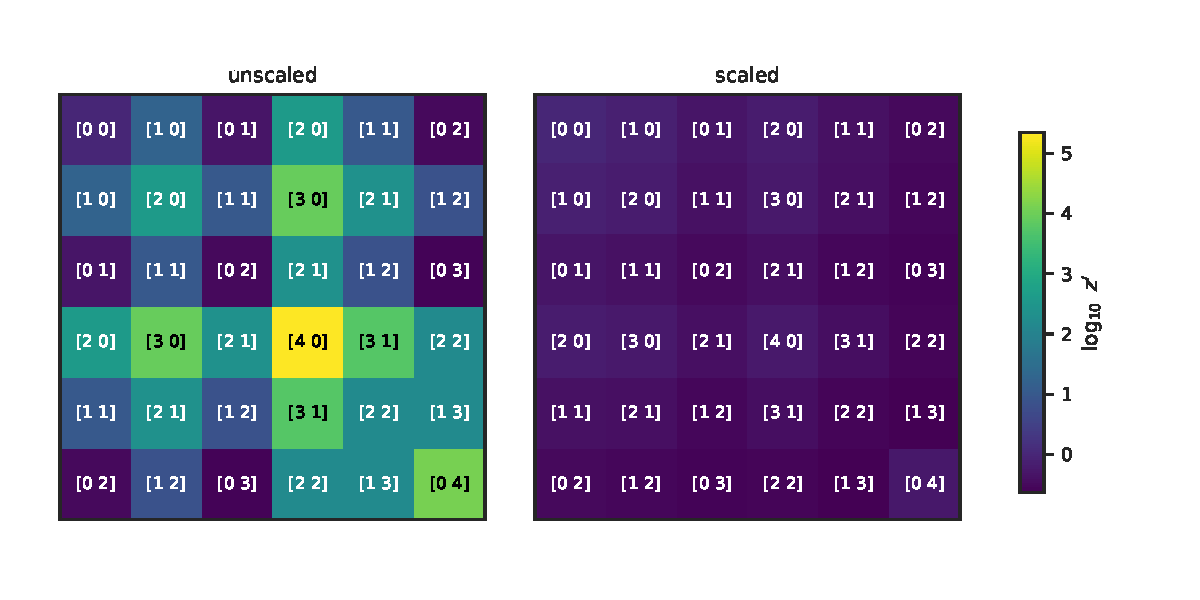
\includegraphics[width=\textwidth]{gfx/magnitudes.pdf}
	\caption[Moment matrix scaling]{The unscaled and scaled value of the moment matrix proxy variable
    $M(\vec{z'})$ after optimization using \acsfont{MOSEK}. The indices are given along the
    logarithmic (base $10$) values. The unscaled version (left) shows large
    differences in magnitudes, while on the scaling suppresses
    these large variations (right). The case study used here is \autoref{model:dim},
    with a threshold $H=25$ for species $M$ and a time-horizon $T=1$. The
    relaxation order $r=2$. Therefore moments of orders up to $2r=4$ appear.}
    \label{fig:magnitudes}
\end{figure}


\subsection{Case Studies}
We implemented and solved the \ac{SDP} programs described above using optimization suite \acsfont{MOSEK} version 9.1.2 \parencite{mosek} via the \acsfont{CVXPY}
interface version 1.0.24 \parencite{cvxpy}.

\subsubsection*{Dimerization}
As a first case study, we use \autoref{model:dim} with parameters $\lambda=100$ and $\delta=0.2$.
In this model, we are interested in the time at which the number of agents of type $M$
surpasses a threshold of $25$ before some time-horizon $T$,
i.e.\ \[
	\tau=\inf\{t\geq 0\mid X_t \geq 25\}\land T\,.
\]
First, we set no finite time-horizon $T$, i.e.\ $T=\infty$.
\marginpar{We can let $T\to\infty$ because this system is ergodic and therefore $\tau<\infty$ a.s.}
This is achieved by dropping the moments $\vec y_2$
of measure $\nu_2$ in the linear constraints~\eqref{eq:sdp_for_fpt}.
This can be done because the threshold on $M$ makes the state-space finite
and therefore the first passage time distribution is a phase-type distribution
which possesses finite moments \parencite[][Chapter 7.6]{stewart2009probability}.

The empirical \ac{FPT} distribution based on \num{100000} \ac{SSA} simulations is given in \autoref{fig:dim_fpt_fpt}
and the bounds, given different moment orders, are given in \autoref{fig:dim_fpt:mfpt}.
As we can see in \autoref{fig:dim_fpt:mfpt}, the bounds capture the \ac{MFPT} precisely for orders \numlist{5;6}.
The difference between upper and lower bound decreases roughly exponentially with increasing relaxation order $r$.
We found that this trend was consistent among the case studies presented here (cf.\ \autoref{fig:convergence}).
\begin{figure}
	\centering
	\subfloat[\ac{FPT} distribution]
    {\label{fig:dim_fpt_fpt}
	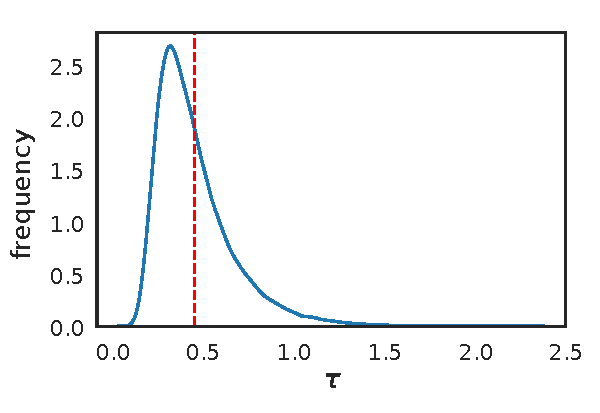
\includegraphics[width=.48\textwidth]{gfx/fpt_dist_dim.pdf}}
	\subfloat[\ac{MFPT} bounds.]
    {\label{fig:dim_fpt:mfpt}%
        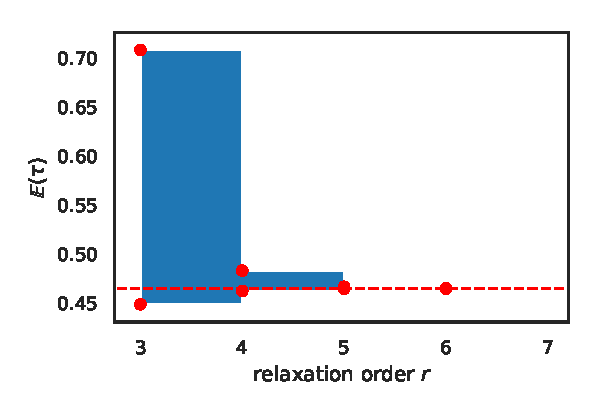
\includegraphics[width=.48\textwidth]{gfx/fpt_bounds_dim.pdf}} \\
	\caption[\ac{FPT} and \ac{MFPT} distribution and bounds]{First-passage time characterisitics for \autoref{model:dim} with $\tau=\inf\{t\geq 0\mid X_t \geq 10\}\land \infty$.
	The dashed red line denotes the sampled \ac{MFPT} based on \num{100000} \ac{SSA} samples. Bounds are based on the \ac{SDP} \eqref{eq:sdp_for_fpt} with different moment orders}
\end{figure}
% \begin{figure}[t]
%     \centering
%     \begin{minipage}{.49\textwidth}
%     \centering
%     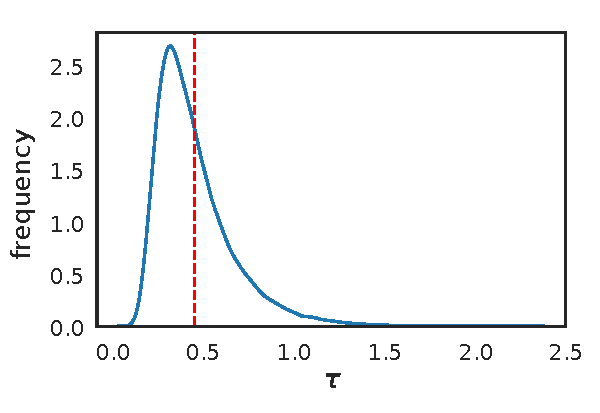
\includegraphics[scale=.6]{gfx/fpt_dist_dim.pdf}\\(a)
%     \end{minipage}
%     \begin{minipage}{.49\textwidth}
%     \centering
%     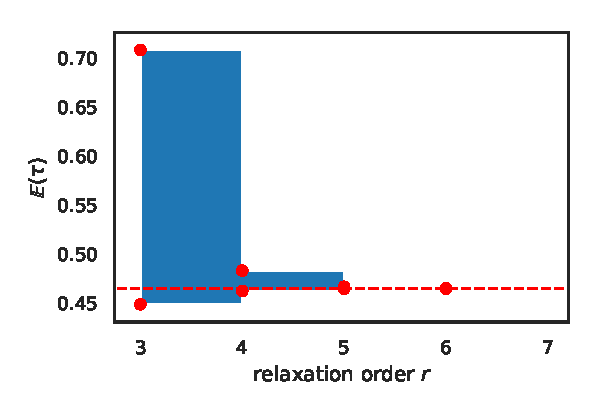
\includegraphics[scale=.6]{gfx/fpt_bounds_dim.pdf}\\(b)
%     \end{minipage}
% 	\caption{    (a) The distribution of $\tau$ estimated based on 100,000 \ac{SSA} samples.
%     (b) The bounds based on the \ac{SDP} in~\eqref{eq:sdp_for_fpt} with different moment
%     orders.\label{fig:dim_fpt}}
% \end{figure}

Next, we look at first passage times within a finite time-horizon $T$.
In \autoref{fig:dim_fpt_fin:mfpt} we summarize the bounds obtained for the \ac{MFPT} over $T$.
While low-order relaxations (light) give rather loose bounds, the bounds are already fairly tight
when using $r=4$.
In many cases, hitting probabilities, that is, the probability of reaching the
threshold before time $T$, are of particular interest.
This is done by switching the optimization objective in~\eqref{eq:sdp_for_fpt} from the mass of the
expected occupation measure $\xi$ to the mass of $\nu_1$.
In terms of moments, the objective changes from $z_{00}$ to $y_{10}$.
The need for such a scenario often aris\-es in the context of model checking, where one might be
interested in the probability of a population exceeding a critical threshold.
By varying the time-horizon, we are able to recover bounds on the cumulative density 
\[
	F(t) = \Pr(X_s=H\mid s<t)
\]
of the first passage time (\autoref{fig:dim_fpt_fin:rp}).
\begin{figure}
    \centering
	\subfloat[\ac{MFPT} bounds over $T$.]
    {\label{fig:dim_fpt_fin:mfpt}
	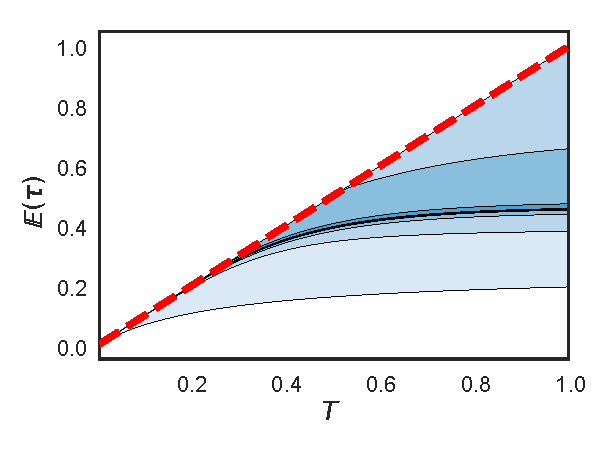
\includegraphics[width=.48\textwidth]{gfx/mfpt_bounds.pdf}}
    \subfloat[Reaching probabilities up to $T$.]
    {\label{fig:dim_fpt_fin:rp}
        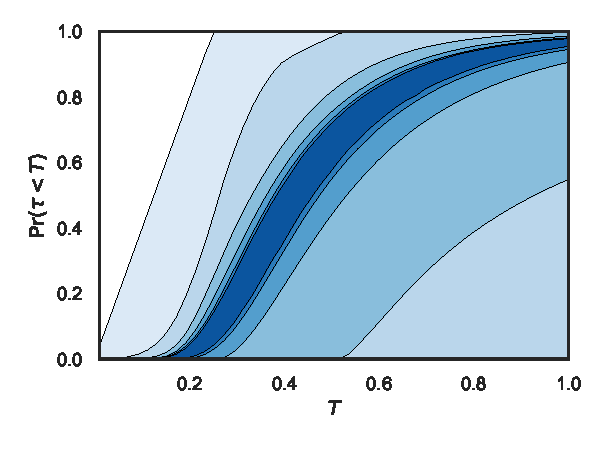
\includegraphics[width=.48\textwidth]{gfx/reachability_probs.pdf}}
	\caption[\acp{MFPT} up to a varying time-horizon]{\Acp{MFPT} and reaching probability bounds for the dimerization model with
    $\tau=\inf\{t\geq 0\mid X_t \geq 25\}\land T$ and varying $T$.
	The results for \ac{SDP} relaxations of orders \num{1} (light) to \num{6} (dark) are shown.\label{fig:dim_fpt_fin}}
\end{figure}
% \begin{figure}[t]
%     \centering
%     \begin{minipage}{.49\textwidth}
%     \centering
%     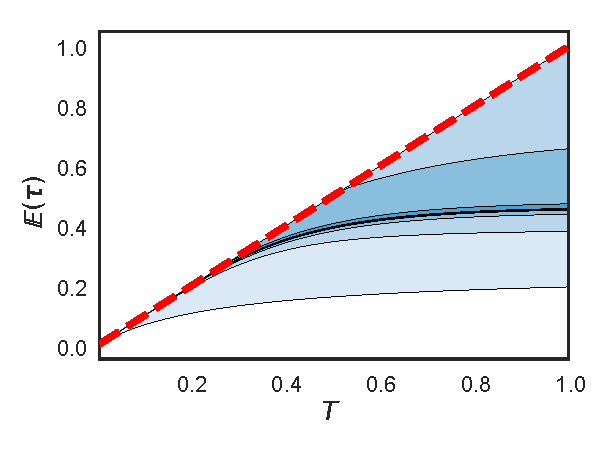
\includegraphics[scale=.6]{gfx/mfpt_bounds.pdf}\\(a)
%     \end{minipage}
%     \begin{minipage}{.49\textwidth}
%     \centering
%     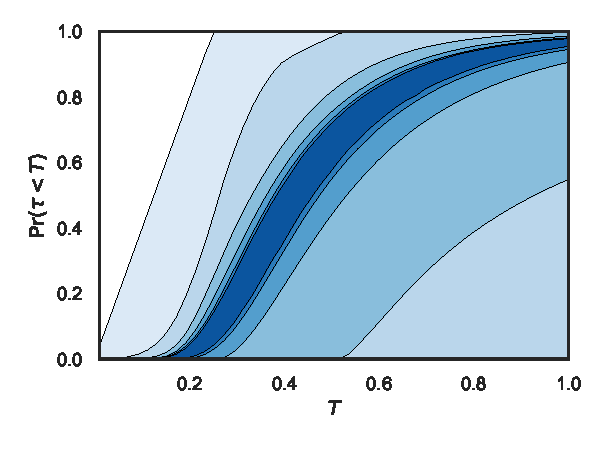
\includegraphics[scale=.6]{gfx/reachability_probs.pdf}\\(b)
%     \end{minipage}
%     % \begin{minipage}{.15\textwidth}
%     % legend
%     % \end{minipage}
%     \caption{First passage times for the dimerization model with
%     $\tau=\inf\{t\geq 0\mid X_t \geq 25\}\land T$.
%     The results for \ac{SDP} relaxations of orders \num{1} (light) to \num{6} (dark) are shown.
%     (a) The bounds on the \ac{MFPT} for differing time-horizons $T$.
%     (b) Bounds on the probability to reach the threshold before time $T$.\label{fig:dim_fpt_fin}}
% \end{figure}

Finally, we look at turn to the dimer species $D$ that is synthesized by the combination of
two monomers $M$. Here, we look at the time until the agents of type $D$ exceed a threshold of five
with a time-horizon $T=1$. Note that we do not limit the number of $M$ agents. Therefore
the analyzed state-space is countably infinite. As in the previous two examples, we
observe a roughly exponential decrease in interval size with increasing relaxation
order $r$ (cf.\ \autoref{fig:convergence} and \autoref{tab:bounds}).


\subsubsection*{Parallel Dimerizations}
As a second study, we consider a two-dimensional model by combining two
independent dimerizations.
\begin{model}[Parallel independent dimerizations]\label{model:double_dim} This model consists of two independent versions of \autoref{model:dim}\turnto{model:dim}.
	\[
		\varnothing\xrightarrow{10^4}M_1\quad 2M_1\xrightarrow{0.1}D_1\quad \varnothing\xrightarrow{10^4}M_2\quad 2M_2\xrightarrow{0.1}D_2
	\]
	Initially, \[0=X_0^{(M_1)}=X_0^{(M_2)}=X_0^{(D_1)}=X_0^{(D_2)}\,.\]
\end{model}
As a \ac{FPT} we consider the time at which either $M_1$ or $M_2$ surpasses a threshold of \num{200} or a time-horizon of $T=10$
is reached, i.e.
\[ \tau=\inf\{t\geq 0\mid X_t^{(M_1)} \geq 200\}\land \inf\{t\geq 0\mid X_t^{(M_2)} \geq 200\}\land 10\,.
\]
As before, we ignore the product species $D_1$ and $D_2$ since they do not influence $\tau$.
% Still, the possible state-space reaches a size of $200^2=\num{40000}$.
% \luca{40000 is very small... I would not emphasize it}\todo{yes, but the only reason for this case study ist that we have a ``larger'' relevant state-space}
The \ac{SSA}   (using $n=\num{10000}$ runs) gives the estimate $\E{\tau}\approx {0.028378}$ %\pm 1.3025e-04$ (99\%-CI)
which is captured tightly by the \ac{SDP} bounds (cf.\ \autoref{tab:bounds}).
For higher relaxation orders $r \geq 5$  numerical issues prevented the solution of the
corresponding \acp{SDP}.

\subsection{Hybrid Models \textit{\&} Multi-Modality}
The analysis of switching times is a particularly interesting case of \acp{FPT} that
arises in many   contexts.
Often mode switching in such systems can be described a modulating Markov process
whose switching rates may depend on the system state (e.g.\ the population sizes).
In biological applications, mode switching often describes a change of the
\acs{DNA} state~\parencite{hasenauer2014method,stekel2008strong} and the analysis of
switching time distribution is of particular interest~\parencite{spieler2014model,barzel2008calculation}.

In the context of \acp{MPM}, typically the state-space $\mathcal{S}=
\mathbb{N}^{\tilde{n}_S}\times {\{0,1\}}^{\hat{n}_S}$.
This state is modeled by  $\hat{n}_S$ population variables with
binary domains. Therefore, at each time point, the state of these modulator variables
is given by a set of Bernoulli random variables.
When considering the moments of
such a variable $X$, clearly
\[
	\E{X^m}=\E{X}=\Pr(X=1)\,,\quad \forall m\geq 1
\]
We can use this fact two ways: We could use the same moment
constraints
as above and impose additional equality constraints on the moments matrices
to ensure $\E{X^m}=\E{X}$, $m\geq 1$.
Alternatively, we can apply this simplification to the moment equation, which we choose here.

We apply a  split of variables $\vec X_t$  into the high count part ${\vec{\tilde{X}}}_t$ and the binary
part ${\vec{\hat{X}}}_t$ to
the expectations in~\eqref{eq:mfpt:mom_ode}. Similarly, we split   $\vec v_j$ and
with a case
distinction over the mode variable,
we arrive at a similar result as in~\parencite{hasenauer2014method}:
\begin{equation}\label{eq:mcm}
\begin{split}
	& \frac{d}{dt}\E{\vec{\tilde{X}}^{{\vec m}}_t 1_{=\vec y}({\vec{\hat{X}}}_t)}\\
   =&\sum_{j=1}^{n_R}
   \E{\left(\left(\vec{\tilde{X}}_t+\vec{\tilde{v}}_j\right)^{\vec
   m}1_{=\vec y}({\vec{\hat{X}}}_t+\vec{\hat{v}}_j)
       -{\vec{\tilde{X}}}_t^{\vec
       m}1_{=\vec y}({\vec{\hat{X}}}_t)\right)\alpha(\vec X_t) }\\
    =&\sum_{j=1}^{n_R}
        \E{{\left(
                {\vec{\tilde{{X}}}}_t+\vec{\tilde{{v}}}_j
            \right)}^{\vec{m}}\alpha_j(\vec{\tilde{{X}}}_t, \vec{{y}} -
            \vec{\hat{v}}_j)
            1_{={\vec{y}- \vec{\hat{v}}_j}}({\vec{\hat{X}}}_t )}\\
    &\quad- \sum_{j=1}^{n_R}
    \E{{\vec{\tilde{{X}}}}_t^{\vec{m}}\alpha_j(\vec{\tilde{{X}}}_t,
                {\vec{y}})
            1_{=\vec y}({\vec{\hat{X}}}_t)}\,.
            \end{split}
\end{equation}
Similarly to the general moment case, we can derive a constraint, by multiplying with a time-weighting factor
and integrating.

For simplicity, here we assume $\tilde n_S=\hat n_S=1$.
Fixing appropriate sequences ${(c_i)}_i$, ${(m_i)}_i$, ${(k_i)}_i$, and
${(y_i)}_i$ the constraint has the following form.\graffito{We fix $0^0=1$.}
\begin{equation}\label{eq:mcm_constraint}
    \begin{split}
	    &\sum_{y\in\{0,1\}}{H}^{m}\E{\tau^k;{{\hat{X}}}_{\tau}= y, \tau
    < T}\\ &\qquad\quad+ T^k\E{{{\tilde{X}}}_T^{m};{{\hat{X}}}_T= y,\tau=T}\\
      =\; &  0^k{{\tilde{x}}}_0^{m} 1_{=  y}({\hat{x}}_0) +
    \sum_i c_i %\sum_{y\in\{0,1\}}
        \E{\int_0^{\tau}t^{k_i}{{{\tilde{X}}}_t}^{{m}_i}\,dt;
            {{\hat{X}}}_t= y_i}\\
    \end{split}
\end{equation}
This way we can decompose the moment matrices such that for each mode $y\in\{0,1\}$,
we have moment matrices composed of the respective partial moments.
To this end, let $z^{(y)}_m$ be the partial moment w.r.t.\ ${{\hat{X}}}= y$.
The moment constraint over the partial moments has a linear structure:
\begin{equation}
0=y_{1k} {H}^{m} - y_{2m}T^k - 0^k x_0^{m}
+\sum_i c_i z^{(y_i)}_{k_i  m_i}\,.
\end{equation}

\begin{table}[t]
\centering
    \caption[\ac{MFPT} bounds]{\ac{MFPT} bounds on \autoref{model:dim}, \autoref{model:double_dim}, \autoref{model:gexpr}.\label{tab:bounds}}
\begin{tabular}{l@{\hspace{1em}}l@{\hspace{1em}}r@{\hspace{2ex}}r@{\hspace{2ex}}r@{\hspace{2ex}}r@{\hspace{2ex}}r}
    \toprule
    & & \multicolumn{5}{c}{relaxation order $r$}\\
        \cmidrule{3-7}
        & & $1$ & $2$        & $3$        & $4$       & $5$       \\
        \midrule
        \autoref{model:dim} & lower & $0.0909$ & $0.2661$ & $0.2845$ & $0.2867$ & $0.2871$ \\
        & upper & $1.0000$ & $0.3068$ & $0.2932$ & $0.2886$ & $0.2875$  \\
         \midrule
         \autoref{model:double_dim} & lower & $0.0010$ & $0.0250$ & $0.0275$ & $0.0280$ & $0.0280$ \\
         & upper & $10.0000$ & $0.0575$ & $0.0323$ & $0.0299$ & $0.0290$ \\
         \midrule
         \autoref{model:gexpr} & lower & $4.0000$ & $6.0028$ & $6.2207$ & $6.3377$ & $6.3772$  \\
         & upper & $10.7179$ & $6.4619$ & $6.4079$ & $6.4004$ & $6.3835$ \\\bottomrule
\end{tabular}
\end{table}

\subsubsection*{Gene Expression with Negative Feedback}
As an instance of a multi-modal system, we consider a simple gene expression with self-regulating
negative feedback which is a common pattern in many genetic circuits~\parencite{stekel2008strong}.

\begin{model}[Negative self-regulated gene expression]\label{model:gexpr}
This model consists of a gene state that is either on or off, i.e.\ $X^{D_{\text{on}}}_t
+X^{D_{\text{off}}}_t = 1$, $\forall t\geq 0$. Therefore the system has two \emph{modes}.
$$
D_{\text{on}} \xrightarrow{\tau_{0}} D_{\text{off}} \quad
D_{\text{off}} \xrightarrow{\tau_{1}} D_{\text{on}} \quad
D_{\text{on}} \xrightarrow{\rho} D_{\text{on}} + P \quad
$$
$$
P\xrightarrow{\delta}\varnothing\quad
P + D_{\text{on}} \xrightarrow{\gamma} D_{\text{off}}
$$
The model parameters are $(\tau_0,\tau_1,\rho,\delta,\gamma)=(10,10,2,0.1,0.1)$ and
$X_0^{(D_{\text{off}})}=1$, $X_0^{(P)}=0$ a.s.
\end{model}

As a first passage time we consider 
\[
	\tau=\inf\{t\geq 0\mid X_t^{(P)} \geq 5\}\land 20\,.
\]


The results are summarized in \autoref{tab:bounds}.
The estimated \ac{MFPT} based on \num{100000}
\ac{SSA} samples is $\E{\tau}\approx 6.37795\pm0.02847$ at $99\%$ confidence level.
Note that our \ac{SDP} solution for $r=5$ yields tighter moment bounds than
the statistical estimation.% based on $100,000$ trajectories.


In \autoref{fig:convergence} we summarize our results about the decrease of the interval widths for increasing relaxation order $r$ by plotting them on a log-scale.
We see an approximately exponential decrease with increasing $r$.
The \acp{SDP} above were all solved within at most a few seconds.
\begin{figure}[t]
    \centering
    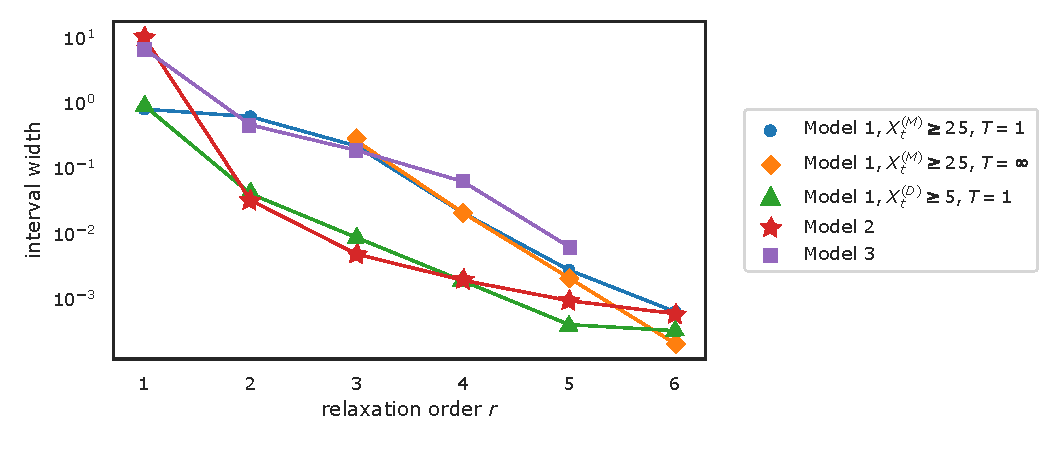
\includegraphics[width=\textwidth]{gfx/convergence.pdf}
	\caption[\ac{MFPT} bound convergence]{The interval width, i.e.\ the difference between upper and lower bound,
    for different case studies and targeted first passage times against the order $r$
    of the \ac{SDP} relaxation.\label{fig:convergence}}
\end{figure}



\section{Conclusion}\label{sec:mfpt:conclusion}
Numerical methods to compute reachability probabilities and first passage times
for continuous-time Markov chains that are based on an exhaustive exploration of the state-space
are exact up to numerical precision. Such methods, however, do not scale and cannot be efficiently applied to models with large or infinite state-spaces,
an issue exacerbated in population models. Moment-based methods offer an alternative analysis approach
for \acp{MPM}, which scales with the number of different populations in the system
but are approximations with little or no control of the error.
In this work,
we bridge this gap by proposing a rigorous approach to derive bounds on first passage
times and reachability probabilities, leveraging a semi-definite programming formulation
based on appropriate moment constraints. 

The method we propose is shown to be accurate in several examples. It does, however, suffer, like all moment-based methods, from numerical instabilities in the \ac{SDP} solver, caused by the fact that moments typically span several orders of magnitude. We proposed a scaling of moments to mitigate this effect. 
However, the scaling only addresses the moment matrices but not the linear constraints
which still contain values with varying orders of magnitudes.
Therefore, we plan as future work to investigate an appropriate scaling for the linear constraints
or to redefine the moment
constraints (e.g.\ using an exponential time weighting~\parencite{dowdy2018dynamic}).
Based on this investigation, we expect to make this approach applicable to
more problems including, for example, the computation of bounds of rare event probabilities.
%Numerical instabilities due to moment values of largely differing orders of magnitudes are a current limitation of all moment-based methods.
We also expect that the development of more sophisticated scaling techniques will  improve approximate moment-based methods.

Furthermore, moment-based analysis approaches have shown to be successful
in a wide range of applications such as optimal control problems or the estimation
of densities~\parencite{lasserre2010moments}.
We expect that our proposed ideas   can be adapted to a wider range
of stochastic models such as stochastic hybrid systems, exhibiting partly deterministic dynamics.


\cleardoublepage\chapter{Linear Control Variates for Monte~Carlo \mbox{Estimation}}\label{ch:cvinsrns}
% \author{Michael Backenk\"ohler\inst{1}, Luca Bortolussi\inst{1,2}, Verena Wolf\inst{1}}
% \authorrunning{M.\ Backenk\"ohler et al.}
% \institute{\inst{1}Saarland University, Germany, \inst{2}University of Trieste, Italy}
% \maketitle
% \begin{abstract}
% Stochastic simulation is a widely used method for 
% estimating quantities in models of chemical 
% reaction networks where uncertainty plays a crucial role.
% However,  reducing  the statistical uncertainty of the corresponding  
% estimators requires the generation of a large number 
% of simulation runs, which is computationally expensive.
% To reduce the number of necessary runs, we propose a
% variance reduction technique based on control variates.
% We exploit  constraints on the statistical moments of the 
% stochastic process
% to reduce the estimators' variances.
% We develop an algorithm that selects appropriate control
% variates in an on-line fashion and demonstrate the efficiency of our approach  on several case studies.
% 
% \keywords{Chemical Reaction Network  \and Chemical Master Equation \and Stochastic Simulation Algorithm
% \and Moment Equations \and Control Variates \and Variance Reduction}
% \end{abstract}
% %
% %
%\section{Introduction}

Analysis approaches based on sampling, such as the \acf{SSA}~\parencite{gillespie1977exact}\turnto{sec:ssa}, can  be applied
independent of the size of the model's state-space. 
However, statistical approaches are costly since a large number
of simulation runs is necessary to reduce the statistical 
inaccuracy of estimators. This problem is particularly severe
if reactions occur on multiple time scales or if the event of interest is rare.
A particularly popular technique to speed up simulations is $\tau$-leaping which applies
multiple reactions in one step of the simulation.
However, such multi-step simulations rely on certain assumptions about
the number of reactions in a certain time interval. These assumptions
are typically only approximately fulfilled and therefore introduce  approximation
errors on top of the statistical uncertainty of the considered point estimators.

Moment-based techniques offer a fast approximation of the statistical moments of the model. 
The exact moment dynamics can be expressed as an infinite-dimensional system of \acp{ODE}, which cannot be directly  integrated for a transient analysis.
Hence, ad-hoc approximations need to be introduced, expressing higher order moments as functions of lower-order ones \parencite{ale2013general,engblom2006computing}.
However, moment-based approaches rely on assumptions about the dynamics that are
often not even approximately fulfilled and may lead to high approximation errors. 
Recently, equations expressing the moment dynamics have also been used as constraints for parameter
estimation \parencite{backenkohler2018moment} and for computing moment bounds using semi-definite programming \parencite{dowdy2018dynamic,ghusinga2017exact}.

In this work, we propose a combination of such moment constraints with the \ac{SSA} approach.
Specifically, we   interpret these constraints as random variables 
that are correlated with the estimators of interest usually given as functions of chemical population variables.
These constraints can be used  as  (linear) \acfp{CV} in order to improve the final estimate and reduce its variance \parencite{lavenberg1982statistical,szechtman2003control}.
The method is easy on an intuitive level: If a control variate
is positively correlated with the function to be estimated then 
we can use the estimate of the variate to
adjust the target estimate.
%more details

The incorporation of control variates into the \ac{SSA}
introduces   additional simulation costs for the calculation of the constraint values.
These values are integrals over time, which we accumulate  based on the
piece-wise constant trajectories.
This introduces a trade-off between the variance reduction that is achieved
by using control variates versus the increased simulation cost.
This trade-off is expressed as the product of the variance reduction ratio
and the cost increase ratio.

For a good trade-off, it is crucial to find an appropriate set of control variates.
Here we propose a class of constraints which is parameterized by a moment vector
and a weighting parameter, resulting in infinitely many choices.
We present an algorithm that samples from the set of all constraints and
proceeds to remove constraints that are either only weakly correlated with the
target function or are redundant in combination with other constraints.

In a case study, we explore different variants of this algorithm
both in terms of generating the initial constraint set and of
removing  weak or redundant constraints.
We find that the algorithm's efficiency is superior to a standard estimation procedure
using stochastic simulation alone
in almost all cases.

Although in this work we focus on  estimating first order moments at
fixed time points, the proposed approach can in principle deal with any property that can
be expressed in terms of expected values such as probabilities
of complex path properties.
Another advantage of our technique is that an increased efficiency is achieved without the price of an additional approximation error as it is the case for methods based on moment approximations or multi-step simulations.

\section{Related Work}\label{sec:cv:related}
\paragraph{State-space Truncations}
If the state-space is finite and small enough one can deal with the underlying Markov
chain directly.
But there are also  cases where the transient distribution has an infinitely large support
and one can still deal with explicit state probabilities.
To this end, one can fix a finite state-space, that should contain most of the
probability~\parencite{munsky2006finite}. Refinements of the method work
dynamically and adjust the state-space according to the transient
distributions~\parencite{andreychenko2011parameter,henzinger2009sliding,mateescu2010fast}.

\paragraph{Moment Approximations}
On the other end of the spectrum there are mean-field approximations, 
which model the mean densities faithfully in the system size limit~\parencite{bortolussi2013continuous}.
In between there are techniques such as moment closure \parencite{singh2006lognormal}, that
not only consider the mean, but also the variance and other higher order moments.
These methods depend on ad-hoc approximations of higher order moments to
close the \ac{ODE} system given by the moment equations.
Yet another class of methods approximate molecular counts continuously and approximate the dynamics in such a continuous space, e.g. the system size expansion~\parencite{van1992stochastic} and the
chemical Langevin equation~\parencite{gillespie2000chemical}.

While the moment closure method uses ad-hoc approximations for high order moments to
facilitate numerical integration, they can be avoided in some contexts.
For the equilibrium distribution, for example, the time-derivative of all moments is equal to zero.
This directly yields constraints that have been used for parameter estimation at
steady-state~\parencite{backenkohler2018moment}
and bounding moments of the equilibrium distribution using semi-definite
programming~\parencite{ghusinga2017estimating,ghusinga2017exact,kuntz2017rigorous}.
The latter technique of bounding moments has been successfully adapted in the 
context of transient analysis~\parencite{dowdy2018dynamic,sakurai2017convex,sakurai2019bounding}.
We adapt the constraints proposed in these works to improve statistical estimations via stochastic
simulation (cf.\ \autoref{sec:cv:moments}).


\paragraph{Monte Carlo Simulation}
While the above techniques give a deterministic output, stochastic simulation generates
single executions of the stochastic process~\parencite{gillespie1977exact}.
This necessitates accumulating large numbers of simulation runs to estimate
quantities.
This adds a significant computational burden. Consequently, considerable effort
has been directed at lowering this cost.
A prominent technique is $\tau$-leaping~\parencite{gillespie2001approximate},
which in one step performs multiple instead of only a single reaction.
Another approach is to find approximations that are specific to the problem at hand,
such as approximations based on time-scale separations~\parencite{cao2005slow,bortolussi2015efficient}.

Recently, multilevel Monte Carlo methods have been applied in to time-inhomogenous
\ac{MPM}~\parencite{anderson2018low}. In this techniques estimates are combined
using estimates of different approximation levels.

% \parencite{goodman2009coupling}

The most prominent application of a variance reduction technique in the context
of stochastic reaction networks is importance sampling~\parencite{kuwahara2008efficient}.
This technique relies on an alteration of the process and then weighting samples
using the likelihood-ratio between the original and the altered process.
% \vw{This sentence stands here a bit lonely. Maybe shortly explain importance sampling? Also: there are papers about importance splitting (does this count as variance reduction technique? I would guess so.)}
% 

% \vw{Warum sagst Du hier nicht kurz etwas über numerische Lösungen der CME und die Schwierigkeiten? Eigentlich wäre numerische Lösung vorzuziehen wenn sie nicht so schwierig wäre}

We refer the reader to \textcite{beentjes2021a} for a recent survey of variance reduction methods applied to \acp{MPM}.



\section{Moment Constraints}\label{sec:cv:moments}
The time-evolution of $\E{f(X_t)}$ for some function $f$ is given by \eqref{eq:mom_ode}\turnto{eq:mom_ode}.
The integration of \eqref{eq:mom_ode} with such functions $f$ is well-known in the context of
moment approximations of \ac{MPM}.
For most models the arising \ac{ODE} system is infinitely large, because the time-derivative of
low order moments usually depends on the values of higher order moments.
To close this system, \emph{moment closures}, i.e.\ ad-hoc approximations of higher order moments
are applied \parencite{schnoerr2015}.
The main drawback of this kind of analysis is that it is not known whether the chosen closure gives
an accurate approximation for the case at hand.
Here, such approximations are not necessary, since we will apply the moment dynamics in the context
of stochastic sampling instead of trying to integrate \eqref{eq:mom_ode}.

Apart from integration strategies,
setting \eqref{eq:mom_ode} to zero has been used as a constraint for parameter estimation at steady-state
\parencite{backenkohler2018moment} and bounding moments at steady-state~\parencite{dowdy2018bounds,ghusinga2017exact,kuntz2017rigorous}.
The extension of the latter has recently lead to the adaption of these constraints
to a transient setting~\parencite{dowdy2018dynamic,sakurai2019bounding}.
These two transient constraint variants are analogously derived by multiplying \eqref{eq:mom_ode}
by a time-dependent, differentiable weighting function $w(t)$ and integrating:

As in the previous chapter,\turnto{eq:exp_constraint} multiplication with $w(t)$ and integration on $[t_0, T]$ yields~\parencite{dowdy2018dynamic,sakurai2019bounding}
\begin{multline}\label{eq:poly_con}
        w(T)\E{f(X_{T})}
        - w(t_0)\E{f(X_{t_0})}
	- \int_{t_0}^{T}\frac{dw(t)}{dt}\E{f(X_t)}\,dt\\
        =\sum_{j=1}^{n_R}\int_{t_0}^{T}w(t)
        \E{\left(f{(X_t + v_j)} - f(X_t)\right)\alpha_j(X_t)}\,dt
\end{multline}
While many choices of $f$ are possible, for this work we will restrict ourselves to
monomial functions $f(x)=x^m$, $m\in\mathbb{N}^{n_S}$
% \vw{ich dachte, m soll ein Vektor sein}
i.e.\ the \emph{non-central} or \emph{raw moments} of the process.
In the context of computing moment bounds via semi-definite programming
the polynomial $w(t)=t^s$~\parencite{sakurai2019bounding}
\marginpar{In \autoref{ch:MFPT} we chose the monomial, such that \eqref{eq:poly_con} would admit the interpretation of temporal moments. Here the exponential is a good choice, because it can model both increasing and decreasing weighting.}
and the exponential $w(t)=e^{\lambda(T - t)}$~\parencite{dowdy2018dynamic}
have been proposed.
While both choices proved to be effective in different case studies, relying solely on the latter choice,
i.e.\ \[
	w(t)=e^{\lambda(T - t)} \] was sufficient.

% Let $$
% % \hat m^{(s)}_f = \int_{t_0}^{T}t^s\E{f(X_t)}\,dt
% % \quad\text{and}\quad
%  {m}^{(\lambda)}_f = \int_{t_0}^{T}e^{\lambda(T - t)}\E{f(X_t)}\,dt\,.
% $$
% We can interpret the constraint value as a random variable $Z$.
% Assuming $f$ and the rate functions are polynomials in $x$ we obtain\vw{der Schritt geht fuer mich zu schnell. Wie genau ist Z definiert?}
% \begin{equation}\label{eq:simpl_pol}
%     \E{Z_p} =\,
%          T^s\E{f(X(T))}
%         - t_0^s\E{f(X(t_0))}
%         - s\hat m^{(s-1)}_f
%         + \sum_{k}c_k\hat{m}^{(s)}_{f_k}
% \end{equation}
% and
% \begin{equation}\label{eq:simpl_exp}
%     \E{Z} =\,
%          \E{f(X(T))}
%         - e^{\lambda T}\E{f(X(t_0))}
%         % + \lambda m^{(\lambda)}_f
%         + \sum_{k}c_k{m}^{(\lambda)}_{f_k}\,,
% \end{equation}
For this chapter, we assume that propensity functions $\alpha_i$ are polynomial.
This restriction is only due to the simplification of only having to record one value for each tuple of moment vector $m$ and weighting coefficient $\lambda$.
Given more complex propensity functions, we would need to accumulate other terms during simulation accordingly.
\marginpar{Contrary to the claim in \textcite[Ch.~2.4.2]{beentjes2021a}, the approach is not restricted to mass-action kinetics.}
By expanding the rate functions and $f$ in \eqref{eq:poly_con} and substituting the
exponential weight function we can re-write \eqref{eq:poly_con} as
\begin{multline}\label{eq:simpl_exp}
        0 =\,
         \E{f(X_{T})}
        - e^{\lambda T}\E{f(X_{t_0})}\\
        + \sum_{k}c_k\int_{t_0}^{T}e^{\lambda(T-t)}\E{X_t^{m_k}}\,dt
\end{multline}
with coefficients $c_k$ and vectors $m_k$ defined accordingly.
Assuming the moments remain finite on $[0,T]$, we can define the random variable
\begin{equation}\label{eq:z}
        Z =\,
         f(X_{T})
        - e^{\lambda T}f(X_{t_0})
        + \sum_{k}c_k\int_{t_0}^{T}e^{\lambda(T-t)}X_t^{m_k}\,dt
\end{equation}
with $\E{Z}=0$.

% Clearly, for $\rho=0$ and $z=0$ \eqref{eq:simpl_pol} and \eqref{eq:simpl_exp}
% are equivalent.
\begin{example}
For \autoref{model:bd} the moment equation for $f(x)=x$ becomes
% \vw{sollte -delta Ex sein}
	\[
		\frac{d}{dt}\E{X_t}=\gamma - \delta\E{X_t}\,.
	\]
The corresponding constraint \eqref{eq:simpl_exp} with $\lambda=0$ gives
	\[
		0=\E{X_T} - \E{X_0} - \gamma T + \delta \int_0^{T} \E{X_t}\,dt\,.
	\]
In this instance the constraint  leads to an explicit function of
the moment over time. If  $X_0=0$ w.p.\ $1$, then \eqref{eq:simpl_exp} becomes
\begin{equation}\label{eq:bd_constraint}
\E{X_T} = \frac{\gamma}{\delta} \left(1 - e^{-\delta T}\right)
\end{equation}
when choosing $\lambda=-\delta$.
% When we use this constraint as a control variate
% for the estimation of the mean at some time point, it has a correlation of $\pm1$.
% Therefore the variance is reduced to zero. This illustrates the benefit of choosing 
% control variates, that are highly correlated with the random variable of interest.
\end{example}


In general, a realization of $Z$ depends on the whole trajectory $\tau=x_0t_1 x_1 t_2 \dots\allowbreak t_n x_n$ over $[t_0,T]$.
Thus, for the integral terms
in \eqref{eq:z} we have to compute sums
\begin{equation}\label{eq:dis_int}
    % \frac{1}{k+1}\sum_{i=1}^n\left(t_{i+1}^{k+1} - t_i^{k+1}\right)s_i^m
    % \quad\text{and}\quad
    \frac{1}{\lambda}\sum_{i=1}^n\left(e^{\lambda(T - t_{i+1})}
    - e^{\lambda(T-t_i)}\right)x_i^{m_k}
\end{equation}
over a given trajectory.
This accumulation is best done during the simulation to avoid storing the whole trajectory.
Still, the cost of a simulation run increases.
For the method to be efficient, the variance reduction (\autoref{sec:cv:var_red}) needs
to overcompensate for this increased cost of a simulation run.
\begin{algorithm}
    \SetKwInOut{Input}{input}
    \SetKwInOut{Output}{output}
    \Input{$\pi_0, T, P, n$}
    \Output{trajectory $\tau$}
    initialize accumulator map $A$ for $P$\;
    \For{$i=1,\dots, n$}{
        $\tau \leftarrow$ empty list, $s\leftarrow$ sample from $\pi_0$, $t\leftarrow 0$\;
        \While{$t<T$}{
        $\tau\leftarrow \text{append}(\tau, (s, t))$\;
            $k\leftarrow$ sample reaction $i$ with probability $\propto\alpha_i(s)$\;
            $\delta\sim \text{Exp}\left(\sum_i \alpha_i(s)\right)$\;
            \For{$(m,\lambda)\in \mathit{keys}(A)$}{
                $A[(m,\lambda)]\leftarrow A[(m,\lambda)] $\\ \hspace*{6em}$+\frac{1}{\lambda}\left(e^{ \lambda(t + \delta)} - e^{ \lambda t }\right)x^m$\;
            }
            $s\leftarrow s + v_k$\;
            $t \leftarrow t + \delta$\;
        }
        update means $\hat{V}$, $\hat{Z}$ and covariances $\hat\Sigma$ using $A$\;
        \For{$(m,\lambda)\in \mathit{keys}(A)$}{$A[(m,\lambda)] \leftarrow 0$}
    }
    \textbf{return} $(\hat{\Sigma},\hat{V}, \hat{Z})$\;
    \caption{\label{alg:ssa_lcv}$\text{SSA}_{\text{CV}}$: \ac{SSA} with accumulator updates}
\end{algorithm}

\section{Control Variates}\label{sec:cv:var_red}
Now, we are interested in the estimation of some quantity $\E{V}$
by stochastic simulation.
Let $V_1,\dots,V_n$ be independent samples of $V$.
Then the sample mean 
\[
	\hat{V}_n =\frac{1}{n}\sum_{i=1}^n V_k
\]
is an estimate of $\E{V}$.  By the central limit theorem
\[
\sqrt{n}\hat{V}_n\xrightarrow{d}N(\E{V},\sigma_V^2)\,.
\]
Now suppose, we know of a random variable $Z$ with $0=\E{Z}$.
The variable $Z$ is called a \emph{\acf{CV}}.
If a \acl{CV} $Z$ is correlated with $V$, we can
use it to
reduce the variance of $\hat{V}_n$~\parencite{glasserman2005large,nelson1990control,szechtman2003control,wilson1984variance}.
For example, consider we are running a set of simulations and consider a single
constraint.
If the estimated value of this constraint is larger than zero and we estimate a positive correlation
between the constraint $Z$ and $V$, we would, intuitively, like to {decrease} our
estimate $\hat{V}_n$ accordingly.
This results in an estimation of the mean of the random variable
\[
	Y_{\beta}= V-\beta Z
\]
instead of $V$.
The variance%\vw{wo kommt das alpha her?Sollte beta sein}
\[
	\sigma_{Y_{\beta}}^2 = \sigma_V^2-2\beta \Cov{V}{Z} + \beta^2\sigma_Z^2\,.
\]
The optimal choice $\beta$ can be computed by  considering the minimum of $\sigma_{Y_\beta}^2$. Then
\[
	\beta^{*}={\Cov{V}{Z}}/{\sigma_Z^2}\,.
\]
Therefore 
\[
	\sigma_{Y_{\beta^{*}}}=\sigma_Z^2(1 - \rho_{VZ}^2)\,,
\]
where $\rho_{VZ}$ is the correlation of $Z$ and $V$.

If multiple control variates are available, we can proceed in a similar fashion.
Now, let ${Z}$ denote a vector of $d$ control variates and let
\[
\Sigma=
\begin{bmatrix}
\Sigma_{ Z} & \Sigma_{V Z}\\
\Sigma_{ Z V} & \sigma_V^2
\end{bmatrix}
\]
be the covariance matrix of $({Z},V)$.
As above, we estimate the mean of
\[
    {Y}_{\beta}=V -{\beta}^{\T}{Z}\,.
    \]
The ideal choice of $\beta$ is the result of an ordinary least squares regression between $V$
and $Z_i$, $i=1,\dots,n$.
Specifically,
\[
	\beta^{*}={\Sigma_{ Z}}^{-1}{\Sigma}_{ Z V}\,.
\]
Then, asymptotically
the variance of the estimator
\begin{equation}
\hat{Y}_{{\beta^*}}=\hat{V}-{\beta^*}^{\top}\hat{ Z}
\end{equation}
is~\parencite{szechtman2003control},
\begin{equation}\label{eq:lcv_asym}
    {\sigma_{\hat Y_{\beta^*}}^2} = (1 - R_{ Z V}^2){\sigma_{\hat V}^2}\,,
\end{equation}
where
\begin{equation*}
    R_{ Z V}^2=\Sigma_{ Z V}\Sigma_{ Z}^{-1}\Sigma_{ Z V} / \sigma_V^2\,.
\end{equation*}
In practice, however, $\beta^*$ is unknown and needs to be replaced by
an estimate $\hat{\beta}$.
Then the estimator
\begin{equation}
\hat{Y}_{\hat{\beta}}=\hat{V}-\hat{\beta}^{\top}\hat{ Z}\,.
\end{equation}
This leads to an increase in the estimator's variance.
Under the assumption of $Z$ and $V$ having a multivariate normal
distribution~\parencite{cheng1978analysis,lavenberg1982statistical}, the variance of the estimator is
\begin{equation}\label{eq:lcv_norm_varred}
    {\sigma_{\hat{Y}_{\hat{\beta}}}^2} = \frac{n - 2}{n - 2 - d}(1 - R_{ ZV}^2){\sigma_{\hat V}^2}\,.
\end{equation}

Clearly, a control  variate is ``good'' if it is highly correlated with $V$.
The constraint in \eqref{eq:bd_constraint} is an example of the extreme case.
When we use this constraint as a control variate
for the estimation of the mean at some time point $t$, it has a correlation of $\pm1$
since it describes the mean at that time precisely.
Therefore the variance is reduced to zero.
We thus aim to pick control  variates that are highly correlated with $V$.

\begin{example} Consider, for example, the above case of the birth-death process.
If we choose \eqref{eq:bd_constraint} as a constraint, it would always yield
the exact difference of the exact mean to the sample mean and therefore have a 
	perfect correlation. Clearly, $\hat\beta$ reduces to \num{1} and $\hat Y_1 = \E{X_t}$.
\end{example}

\section{Moment-Based Variance Reduction}\label{sec:cv:algo}
We propose an adaptive estimation algorithm (\autoref{alg:ssa:lcv}) that starts out with
an initial set of control variates
and periodically removes potentially inefficient variates.
The ``accumulator set'' $A$ represents the time-integral terms \eqref{eq:dis_int}.
The size of $A$ has the most significant impact on the overall speed of the algorithm
since it represents the only factor incurring a direct cost increase in the \ac{SSA} itself (\autoref{line:run_ssa}).

The algorithm consists of a main loop which performs $n$ simulation runs (\autoref{line:main_loop}).
Between each run the mean and covariance estimates of $[Z,\;  V]$ are updated (\autoref{line:updates}).
Every $d<n$ iterations, the control variates are checked for  \emph{efficiency}
and \emph{redundancy} (lines \ref{line:cond_ck_begin}--\ref{line:cond_ck_end}).
\begin{figure}[htb]
	\centering
	\subfloat[$\E{X^A_2}$ in \autoref{model:dim}]
	{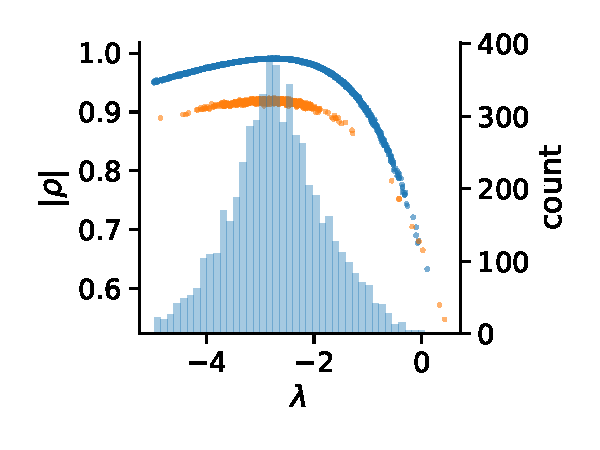
\includegraphics[scale=0.55]{gfx/cs_bdim.pdf}}
	\subfloat[$\E{X^X_{50}}$ in \autoref{model:dm}]
	{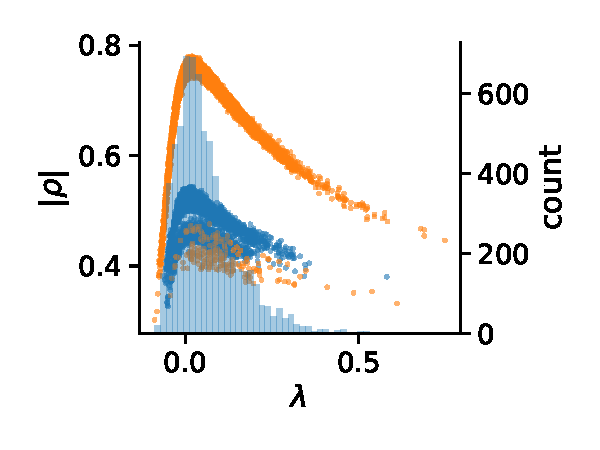
\includegraphics[scale=0.55]{gfx/cs_pm.pdf}}
	\caption[\ac{CV} correlation charactersitics]{The absolute correlation of different constraints {to $V$}
    arising from different choices of $\lambda$. The blue dots represent constraints
    based on first order moments, while the orange refers to control  variates derived from second
	order moments. In both cases $\num{10000}$ samples were used with
	\num{30} initial samples for $\lambda$ from $N(0,1)$ and $k_{\min}=2$. A quadratic decision bound was used for
    the redundancy removal. Furthermore, a histogram of control  variates selected by \autoref{alg:ssa:lcv}
    is given.
    In (a) $\E{X^A_2}$ in the dimerization model was estimated.
    In (b) $\E{X^X_{50}}$ in the distributive modification model was estimated.
    }
    \label{fig:bdim}
\end{figure}

Checking both conditions is based on the correlation $\rho_{ij}$ between the $i$-th and $j$-th control variate
and the correlation $\rho_{iv}$ of a control variate $i$ to $V$.
These are elements of the correlation matrix
\[
C=
\begin{bmatrix}
1 & \dots & \rho_{1k} & \rho_{1v} \\
\vdots & \ddots & \vdots & \vdots \\
\rho_{k1} & \dots & 1 & \rho_{kv} \\
\rho_{v1} & \dots & \rho_{vk} & 1
\end{bmatrix}\,.
\]
The first condition is a simple lower threshold $\rho_{\min}$ for a correlation $\rho_{iv}$.
This condition aims to remove those variates  from the control  variate set that are only weakly correlated to $V$ (\autoref{line:weak_covs}).
The rationale is that, if variate $i$ has a low correlation with the variable of interest $V$,
its computation may not be worth the costs.
Here, we propose to set $\rho_{\min}$ heuristically as
\[
	\rho_{\min} = \min\left(0.1, \frac{\max_{i}\rho_{iv}}{k_{\min}}\right)\,,
\]
where $k_{\min}>1$ is an algorithm parameter.

The second condition aims to remove redundant conditions.
This is not only beneficial for the efficiency of the estimator, but also 
necessary for the matrix inversion \eqref{eq:lcv_asym}
because perfectly and highly correlated constraints will make
the covariance matrix estimate $\hat{\Sigma}_Z$ (quasi-) singular.
For all considered criteria we iterate over all tuples $(i,j)\in \{1,\dots,k\}^2$, $i\neq j$,
removing the weaker of the two, i.e.\ $\argmin_{k\in\{i,j\}}\rho_{kv}$,
if the two control  variates are considered redundant (\autoref{line:redundant_covs}).

There are many ways to define such a redundancy criterion.
Here, we focus on criteria that are defined in terms of the
average correlation \[ \bar\rho_{ij}=(\rho_{iv} + \rho_{jv})/2\,.\]
For two variates $i$ and $j$ we then check if their mutual correlation
$\rho_{ij}$ exceeds a some function $\phi$ of ${\bar{\rho}}_{ij}$,
i.e.\ we check the inequality
\[
	\phi(\bar\rho_{ij}) \leq \rho_{ij}\,.
\]
If this inequality holds, constraint $\argmin_{k\in\{i,j\}}\rho_{kv}$ is removed.
Naturally, there are many possible choices for the above decision boundary $\phi$ (cf.\ \autoref{fig:decision}).


The simplest choice is to ignore $\bar\rho_{ij}$ and just fix a constant close to $1$ as a threshold,
e.g.\ \[ \phi_c(\bar\rho_{ij})=0.99\,.\] While this often leads to the strongest variance reduction
and avoids numerical issues in the control variate computation, it turns out
that the computational overhead is not as well-com\-pen\-sa\-ted as by other choices of $\phi$ (see \autoref{sec:cv:study}).

Another option is to fix a simple linear function, i.e.\ \[ \phi_{\ell}(\bar\rho_{ij})=\bar\rho_{ij}\,.\]
For this choice the intuition is, that one of two constraints is removed if their mutual
correlation exceeds their average correlation with $V$.


Here, we also assess two quadratic choices for $\phi$. The first choice of
\[
	\phi_{q}(\bar\rho)=1 - (1-\bar\rho)^2
\]
is more tolerant than the linear function and more strict than a threshold function, except for
highly correlated control  variates.
Another variant of $\phi$ is given by including the lower bound $\rho_{\min}$ and scaling
the quadratic function accordingly:
\[ \phi_{\mathit{sq}}(\bar\rho)=1-((1-\bar\rho)/(1-\rho_{\min}))^2\,.\]
The different choices of $\phi$ considered here are plotted in \autoref{fig:decision}.
\begin{algorithm}[ht]
\SetKwInOut{Input}{input}
\SetKwInOut{Output}{output}
\Input{$n, d, n_{\max}, n_{\lambda}, k_{\min}$}
\Output{an estimate using linear control variates}
  $L\leftarrow\{\lambda_i\sim \pi_\lambda \mid 1\leq i< n_{\lambda} \} \cup \{ 0 \}$\label{line:lambda_sample}\;
  $P \leftarrow \{ ({m}, \lambda) | 1\leq\lvert {m} \rvert \leq n_{\max}, \lambda\in L\}$\label{line:init_covs}\;
  \For{$i=1,\dots,\lfloor n/d \rfloor$\label{line:main_loop}}{
      $(\hat{\Sigma}_i, \hat{V}_i, \hat{Z}_i) \leftarrow \text{SSA}_{\text{CV}}(\pi_0,T,P,d)$\label{line:run_ssa}\;
     update $\hat\Sigma$, $\hat{V}$, and $\hat{Z}$\label{line:updates}\;
  		$\rho_{\min}\leftarrow \min\left(0.1,{\max_i \rho_{iv}}/{k_{\min}}\right)$\label{line:cond_ck_begin}\;
  		$P\leftarrow P\setminus\{({m}_k, \lambda_k)\mid \rho_{kv} < \rho_{\min}\}$\label{line:weak_covs}\;
  		$P\leftarrow P\setminus\{({m}_k, \lambda_k)\mid \exists i,j.i\neq j,
  		\phi(\bar\rho_{ij}) < \rho_{ij},$ \label{line:redundant_covs}\\
		\hspace{10em}$k=\argmin_{k\in\{i,j\}}\rho_{kv}\}$\label{line:cond_ck_end}\;
  	}
% % \State $\hat{\beta}\leftarrow\hat\Sigma_{{Z}}^{-1}\hat\Sigma_{{Z}V}$
\Return $\hat{V} - {(\hat{\Sigma}_{{Z}}^{-1}\hat\Sigma_{{Z}V})}^{\top}\hat{{Z}}$\label{line:compute_lcv}\;
    \caption{\label{alg:ssa:lcv}Estimate the mean of species $i$ at time $T$}
\end{algorithm}
\begin{figure}[htb]
    \centering
    \begin{minipage}{.6\textwidth}
    \centering
    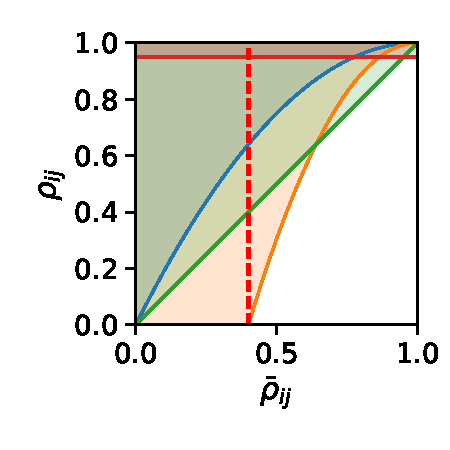
\includegraphics[scale=.6]{gfx/decision_funcs.pdf}
    \end{minipage}
    \hspace{-2.8em}
    \begin{minipage}{.3\textwidth}
    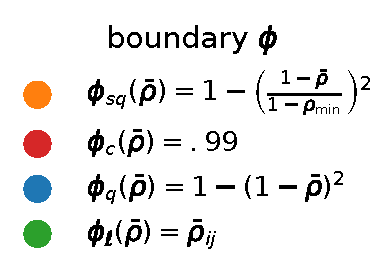
\includegraphics[scale=.6]{gfx/legend_1.pdf} \vfill
    \end{minipage}
	\caption[\ac{CV} redundancy heuristics]{Different decision functions
    used in the redundant control  variate removal. The weaker of any two control  variates is removed if
    the pair $(\bar\rho_{ij}, \rho_{ij})$ belongs to the shaded area of the considered function.
    The vertical dashed line indicates $\rho_{\min}$.\label{fig:decision}}
\end{figure}


Now, we discuss  the choice of the initial control  variates. We identify control  variate $k$ by
a tuple $({m}_k, \lambda_k)$ of a moment vector ${m}_k$
% \vw{vorher war $m_k$ ein vektor mit integern}
and a time-weighting
parameter $\lambda_k$.
% \vw{refer to equation?}
That is, we use $w(t)=e^{\lambda_k(T-t)}$ and $f(x)=x^{m_k}$ in \eqref{eq:poly_con}.
For a given set of parameters $L$, we use all moments up to some fixed order $n_{\max}$ (\autoref{line:init_covs}).
The ideal set of parameters $L$ is generally not known. 
For certain choices the correlation of the control  variates and the variable of interest is
higher then for others.
To illustrate this, consider the above example of the birth-death process.
Choosing $\lambda=-\delta$ leads to a control variate that has a correlation of $\pm 1$ with
$V$. Therefore, the ideal
choice of initial values for would be $L=\{-\delta\}$.
This, however, is generally not known.
Therefore, we sample a set of $\lambda$'s
from some fixed distribution $\pi_{\lambda}$ (\autoref{line:lambda_sample}).
\begin{figure}[htb]
    \centering
    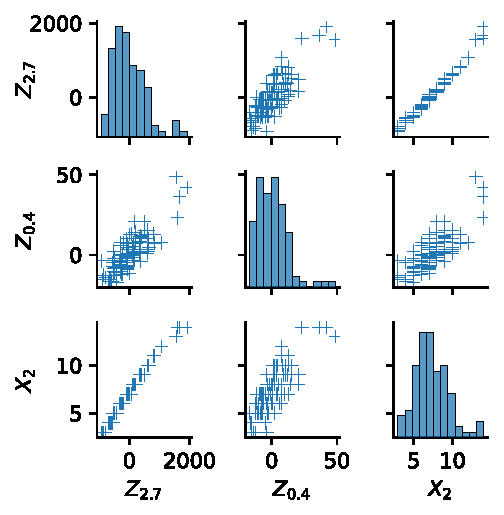
\includegraphics[scale=.65]{gfx/correlation.pdf}
    \hspace*{2em}
    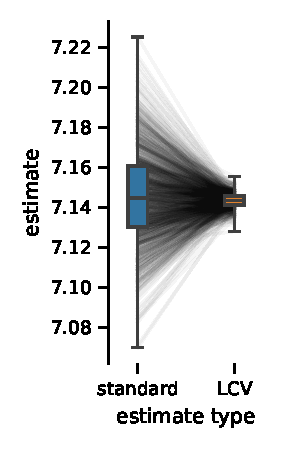
\includegraphics[scale=.65]{gfx/adjustment.pdf}
    \caption[\ac{CV} mean estimates v.\ std.\ mean estimates]{The effect of including \acp{CV} on the mean estimates $\hat{E}(X^M_2)$ in the dimerization case study. Parameters were ${\pi}_{\lambda}=N(0,1)$, ${n}_{\lambda}=30$, ${k}_{\min}=4$, $\phi(\bar\rho)=1-{(1 - \bar\rho)}^2$.}
\end{figure}


% \begin{itemize}
%     \item \textbf{Choice of control variates}
%     \item What needs to be logged.
%     \item Variance, Mean accumulation between runs
%     \item Choice of $\rho$ is done as the largest negative
%         eigenvalue of $Q$ \parencite{dowdy2018dynamic}.
% \end{itemize}

\section{Case Studies}\label{sec:cv:study}
We first define a criterion of \emph{efficiency} in order to estimate
whether the reduction in variance is worth the increased cost.
A natural baseline of a variance reduction is, that it is more efficient to pay for
the computational overhead of the reduction than to generate more samples to achieve a similar
reduction of variance.
Let $\sigma_Y^2$ be the variance of $Y$.
% https://statweb.stanford.edu/~owen/mc/Ch-var-basic.pdf
% Then the variance of the mean, based on $n$ iid.\ samples is $\sigma_Y^2/n$.
% If we let $c_0$ be the cost (i.e.\ CPU time) of a single simulation run, the overall cost to
% achieve this variance is $nc_0$.
% To achieve a variance $\tau^2$, $\sigma_Y^2/\tau^2$ samples are necessary at a cost of
% $c_0\sigma_Y^2/\tau^2$. We can analogously argue for the \ac{cv} estimate where the
% cost of a single iteration is $c_1$.
The \emph{efficiency} of the method is the ratio of the necessary
cost to achieve a similar reduction with the \ac{CV} estimate $Y_{\text{CV}}$ compared to
the standard estimate $Y$~\parencite{l1994efficiency}, i.e.
\begin{equation}\label{eq:efficiency}
E=\frac{c_0\sigma_Y^2}{c_1\sigma^2_{Y_{\text{CV}}}}\,.
\end{equation}
This is the ratio between \emph{slowdown} $c_0/c_1$ and variance reduction $\sigma_{Y}^2 / \sigma_{Y_{\text{CV}}}^2$.
That ratio $c_0/c_1$ depends heavily on both the specific implementation and the technical setup.
The cost increase is  mainly due to the computation of the integrals in \eqref{eq:simpl_exp}.
But the repeated checking of control  variates for efficiency also increases the cost.
The accumulation over the trajectory directly increases the cost of a single simulation
which is the critical part of the estimation.
To estimate the base-line cost $c_0$, $2000$ estimations were performed without
considering any control variates.

The simulation is implemented in the Rust programming language\marginpar{\url{www.rust-lang.org}}.
The model description is parsed from a high level specification. 
Rate functions are compiled to stack programs for fast evaluation.
Code is made available online \parencite{cme-simulation-github}.

We consider four non-trivial case studies. Three models exhibit complex multi-modal behaviour.
We now describe the models and the estimated quantities in detail.

The first model\graffito{This model appeared earlier as \autoref{model:dim} on page~\pageref{model:dim}.} is a simple dimerization on a countably infinite state-space.
\begin{model}[Dimerization]\label{model:dim2}
We first examine a simple dimerization model on an unbounded state-space.
	\[\varnothing\xrightarrow{10}M\,,\quad 2M\xrightarrow{0.1}D\]
with initial condition $X_0^M=0$.
\end{model}
Despite the models simplicity, the moment equations are not closed for this system
due to the second reaction which is non-linear.
Therefore a direct analysis of the expected value would require a closure.
For this model we will estimate $\E{X^M_2}$.

The following two models are bimodal, i.e.\ they each posses two stable regimes
among which they can switch stochastically.
For both models we choose the initial conditions such that the process
will move towards either attracting region with equal probability.
% This complex behaviour makes estimation particularly interesting, since
\begin{model}[Distributive Modification]\label{model:dm}
The distributive modification model was introduced in \parencite{cardelli2012cell}.
It consists of the reactions
\begin{gather*}
	X + Y \xrightarrow{\num{.001}} B + Y\,,\quad
	B + Y \xrightarrow{\num{.001}} 2 Y\\
	Y + X \xrightarrow{\num{.001}} B + X\,,\quad
	B + X \xrightarrow{\num{.001}} 2 X
\end{gather*}
with initial conditions $X^X_0=X^Y_0=X^B_0=100$.
\end{model}

% \begin{model}[Processive Modification]
% \parencite{cardelli2012cell}
% \begin{center}
% \begin{tabular}{c@{\hskip 1.5em}c@{\hskip 1.5em}c@{\hskip 1.5em}c}
%     $X + Y \xrightarrow{0.01} B + Y \,,$&
%     $X \xrightarrow{0.01} B       \,,  $&
%     $Y + X \xrightarrow{0.01} C + X\,, $&
%     $Y \xrightarrow{0.01} C \,,$\\

%     \rule{0pt}{4ex}$B + Y \xrightarrow{0.01} 2 Y \,,  $ &
%     $B \xrightarrow{0.01} Y    \,,   $&
%     $C + X \xrightarrow{0.01} 2 X\,, $ &
%     $C \xrightarrow{0.01} X       $
% \end{tabular}
% \end{center}
% with initial conditions $X_X(0)=10,\!000$ and all other species at $0$.
% \end{model}

\begin{model}[Exclusive Switch]\label{model:es}
	The exclusive switch model consists of \num{5} species, \num{3} of which are typically binary (activity states of the genes) \parencite{loinger2007stochastic}.
\begin{gather*}
	D + P_1 \xrightarrow{\beta} D.P_1\,,\quad
	D.P1 \xrightarrow{\gamma_1} D + P_1  \,,\\
	D + P_2 \xrightarrow{\beta} D.P_2 \,,\quad
	D.P2 \xrightarrow{\gamma_2} D + P_2 \,,\\
	D.P_1 \xrightarrow{\rho_1} D.P_1 + P_1\,, \quad
    D.P_2 \xrightarrow{\rho_2} D.P_2 + P_2\,,\\
	D \xrightarrow{\rho_1} D + P_1\,,\quad
	D \xrightarrow{\rho_2} D + P_2\,,  \quad
	P_1 \xrightarrow{\lambda}\varnothing  \,,\quad
    P_2\xrightarrow{\lambda} \varnothing
\end{gather*}
with initial conditions 
	\[X^D_0=1 \text{ and } X^{D.P1}_0=X^{D.{P_2}}_0=X^{P_1}_0=X^{P_2}_0=0\,.\]
\end{model}

We evaluate the influence of algorithm parameters, choices of distributions
to sample $\lambda$ from, and the influence of the sample size on the efficiency of
the proposed method.
Note that the implementation does not simplify the constraint representations
or the state space according to stoichiometric invariants or limited
state spaces.
\autoref{model:dm}, for example has the invariant 
\[
	X^X_t+X^Y_t+X^B_t=\text{const.}$, $\forall t\geq 0\,,
\]
which could be used to reduce the state-space dimensionality to two.
In \autoref{model:es} the invariant 
\[
	\forall t\geq 0.X^D_t,X^{D.{P_1}}_t,X^{D.{P_2}}_t\in\{0,1\}
\]
could be used to optimize the algorithm by eliminating redundant moments, e.g.\ $\expSym({(X^D)}^2)=\E{X^D}$.
Such an optimization would further increase the efficiency of the algorithm.




We first turn to the choice of the $\lambda$ sampling distribution. Here we
consider two choices:
\begin{enumerate}
    \item a standard normal distribution $N(0,1)$,
    \item a uniform distribution on $[-5,5]$.
\end{enumerate}
We deterministically include $\lambda=0$ in the constraint set, as this parameter
corresponds to a uniform weighting function.
We performed estimations on the case studies using different valuations of the
algorithm parameters of the minimum threshold $k_{\min}$ and
the number of $\lambda$-samples $n_{\lambda}$.
We used samples size $n=\num{10000}$ and checked the control  variates every $d=100$ iterations
for the defined criteria.
For each valuation \num{1000} estimations were performed.
In \autoref{fig:efficiencies_prior}, we summarize the efficiencies
for the arising parameter combinations on the three case studies.
Most strikingly, we can note that the efficiency was consistently larger than one in
all cases.
Generally, the normal sampling distribution out-performed the 
alternative uniform distribution, except in case of the dimerization.
The reason for this becomes apparent, when examining \autoref{fig:bdim}:
In case of the dimerization model the most efficient constraints are found for
$\lambda\approx -3$, while in case of the distributive modification they are located
 just above $0$ (we observe a similar pattern for the exclusive switch case study).
Therefore the sampling of efficient $\lambda$ values is more likely
using a uniform distribution for the dimerization case study, than it is for the others.
Given that larger absolute values for $\lambda$ seem unreasonable due 
their exponential influence on the weighting function and the problem of fixing
a suitable interval for a uniform sampling scheme, the choice of a standard normal
distribution for $\pi_{\lambda}$ seems superior.
\begin{figure}[htb]
    \centering
    \begin{minipage}{0.6\textwidth}
        \vfill
    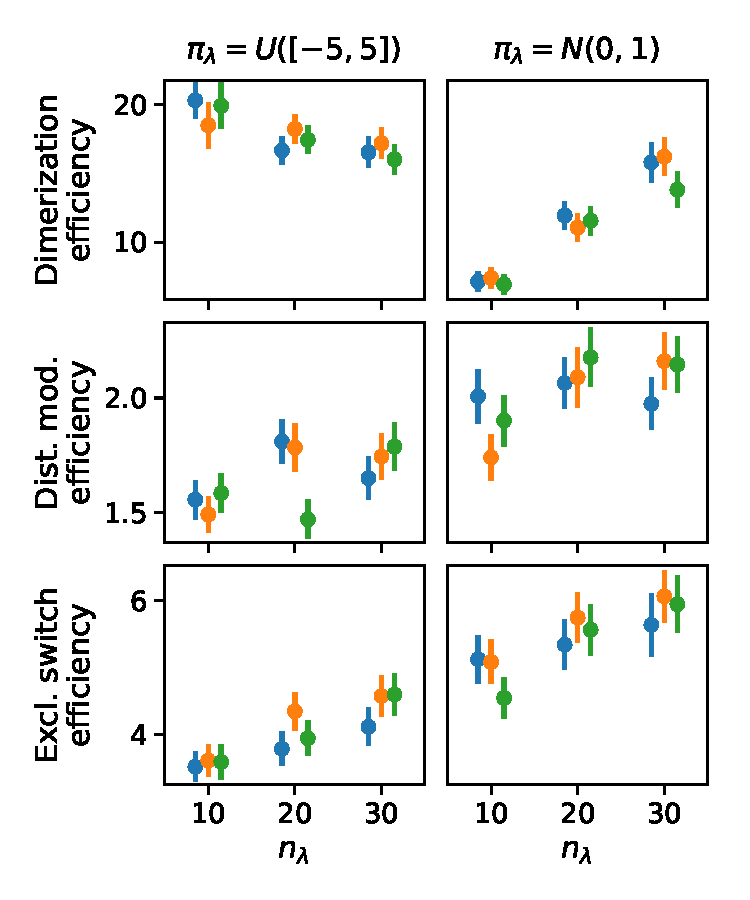
\includegraphics[scale=.5]{gfx/efficiency_priors.pdf}
    \vfill
    \end{minipage}
    \begin{minipage}{0.2\textwidth}
        \vfill
    
\includegraphics[scale=.7]{gfx/legend.pdf}
        \vfill
    \end{minipage}
	\caption[Estimates for varying ${n}_{\lambda}$ and ${k}_{\min}$]{The efficiencies for different valuations of ${n}_{\lambda}$ and ${k}_{\min} $
	and choices of ${\pi}_{\lambda}$. The sample size was $n=\num{10000}$ in all cases
    with $d=100$.
    The bars give the bootstrapped ($1000$ iterations) standard deviations.\label{fig:efficiencies_prior}}
\end{figure}

In \autoref{fig:efficiencies_order} we compare efficiencies for
different maximum orders of constraints $n_{\max}$.
This comparison is performed for different choices
of the redundancy rule and initial $\lambda$ sample sizes $n_{\lambda}$.
Again, for each parameter valuation \num{1000} estimations were performed.
With respect to the maximum constraints order $n_{\max}$ we see a clear
tendency, that the inclusion of second order
constraints lessens the efficiency of the method.
In case of a constant redundancy threshold it even dips below break-even
for the distributive modification case study.
This is not surprising, since the inclusion of second order moments
increases the number of initial constraints quadratically
and the incurred cost, especially of the first iterations,
lessens efficiency.
\begin{figure}[htb]
    \centering    
    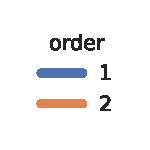
\includegraphics[scale=.55]{gfx/legend_orders.pdf}\\
    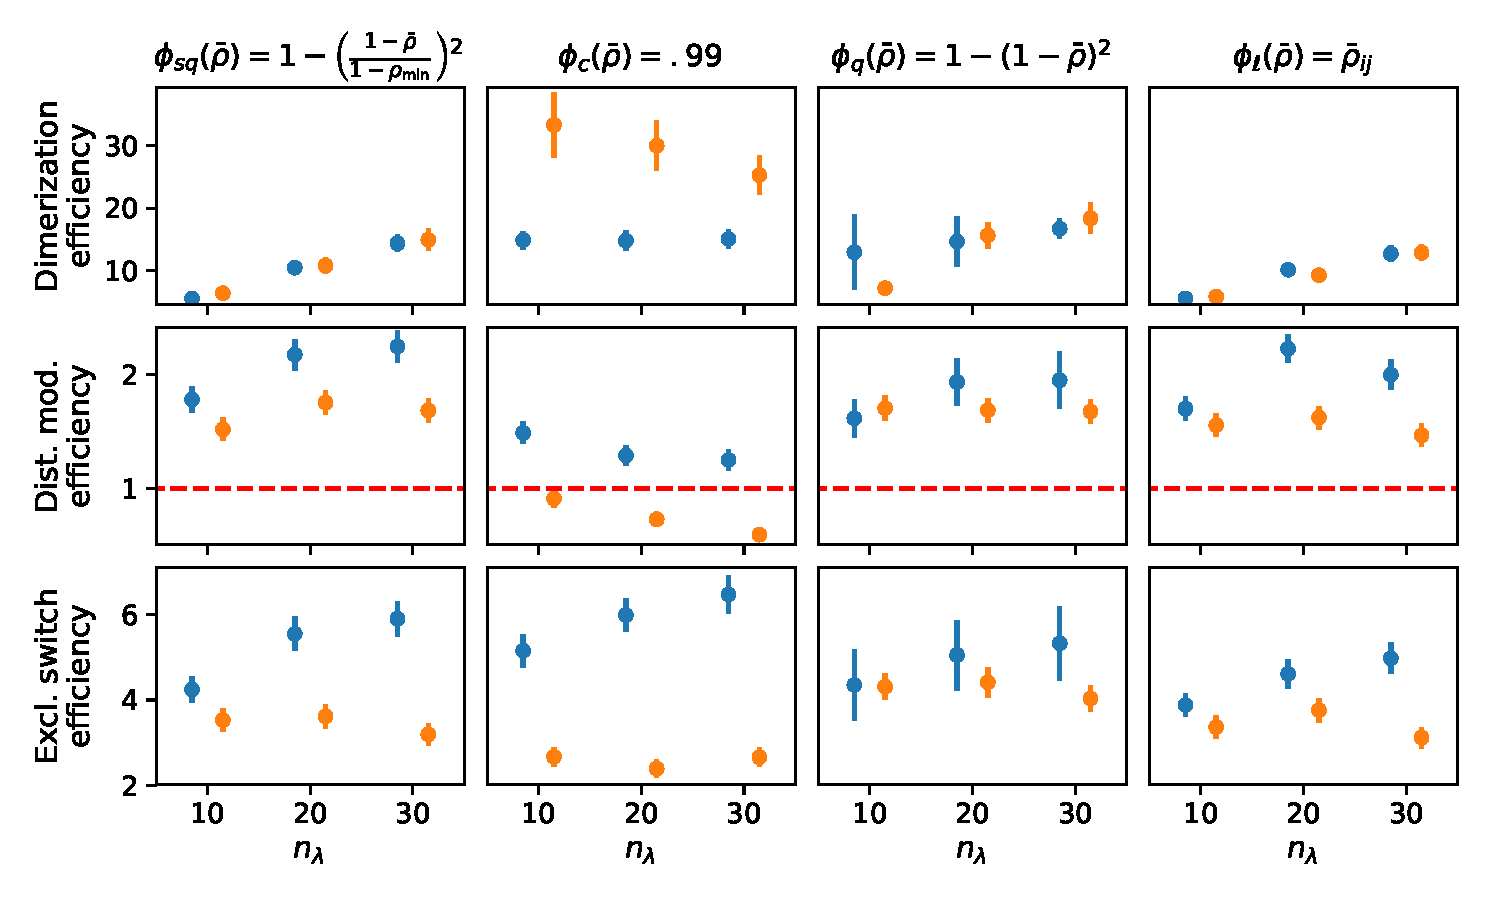
\includegraphics[scale=.4]{gfx/efficiency_ord1.pdf}
	\caption[Estimates for varying redundancy heuristics
	and moment orders]{The efficiency for different redundancy policies $\phi$ and maximal 
	moment orders $n_{\max}$. The sample size was $n=\num{10000}$ in all cases
    with $d=100$. Furthermore, $k_{\min}=3$, $\pi_\lambda=N(0,1)$, and $n_{\max}=1$.
    The bars give the 
    bootstrapped ($1000$ iterations) standard deviations.\label{fig:efficiencies_order}}
\end{figure}
\begin{figure}[htb]
    \centering    
    
\includegraphics[scale=.55]{gfx/legend_horiz.pdf}\\
    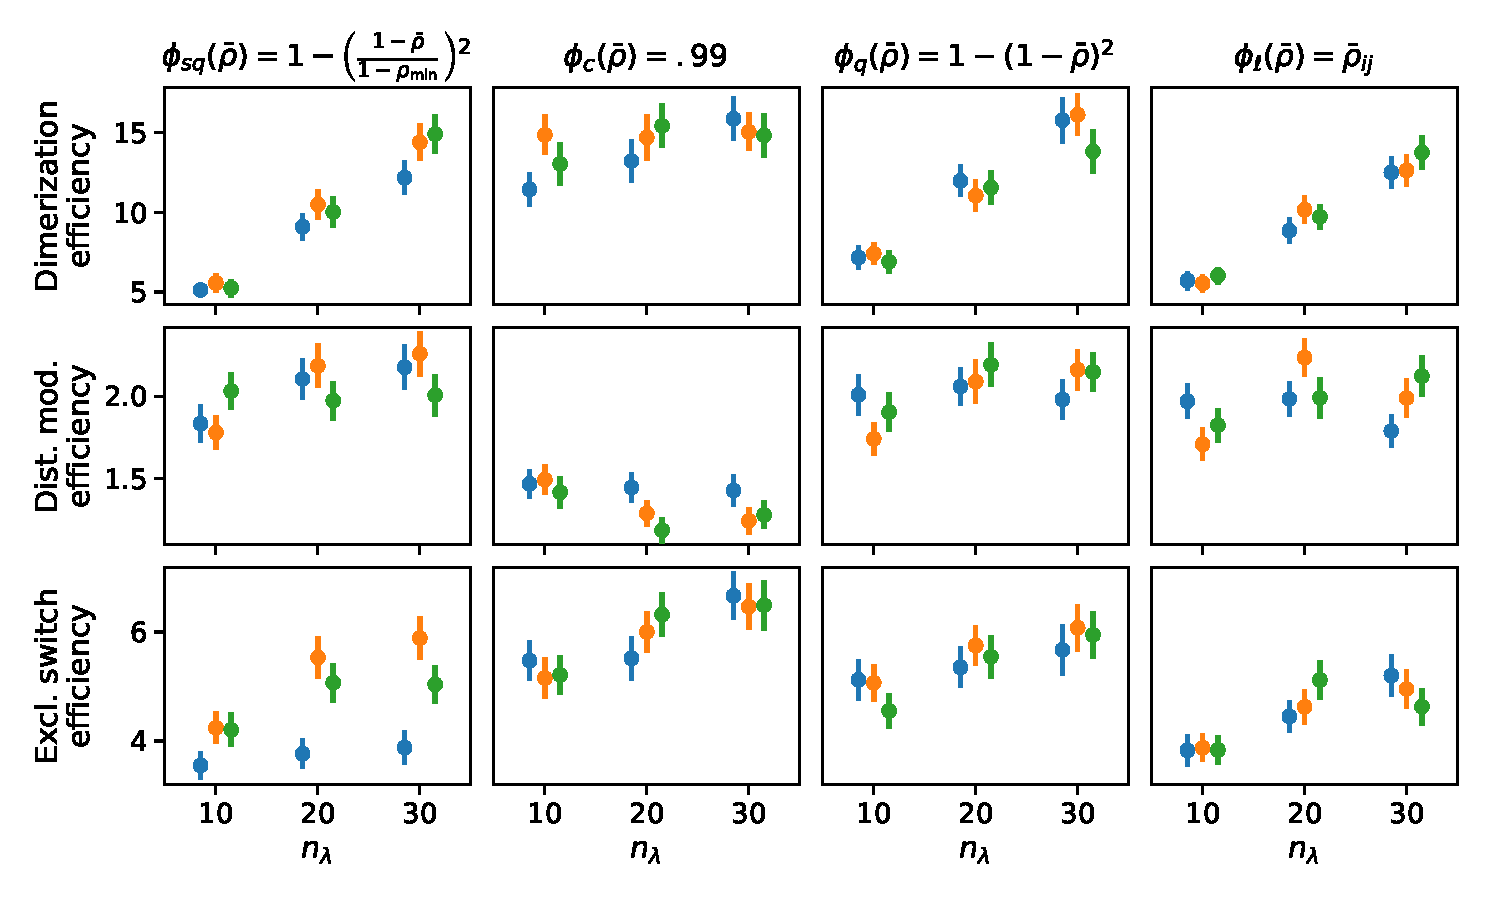
\includegraphics[scale=.4]{gfx/efficiency_pminfrac.pdf}
	\caption[Varying redundancy heuristics and $k_{\min}$]{The empirical efficiencies for different $n_\lambda$ and $k_{\min}$.
	On the considered case studies. The sample size was $n=\num{10000}$ in all cases
    with $d=100$.
	$\num{1000}$ estimations were performed for each case.
    The bars give the 
	bootstrapped (\num{1000} iterations) standard deviations.
    The break-even $E=1$ is marked by the dotted red line.\label{fig:efficiencies_alg_params}}
\end{figure}



\autoref{fig:trade_off} depicts the trade-off between the variance reduction $\sigma_0^2/\sigma_1^2$
versus the cost ratio $c_0/c_1$. Comparing the redundancy criterion based on a constant threshold
$\phi_c$ to the others,
we observe both a larger variance reduction and an increased cost. This is due to the fact, that
more control  variates are included throughout the simulations (\autoref{tab:eff1}, \autoref{tab:eff2}, \autoref{tab:eff3}). Depending on the sample distribution $\pi_{\lambda}$
and the case study, this permissive strategy may pay off. In case of the dimerization, for example,
it pays off, while in case of the distributive modification it leads to a lower efficiency ratio.
In the latter case the model is more complex, and therefore the set of initial
control  variates is larger. With a more permissive redundancy strategy, more control  variates are kept
(ca.\ $10$ when using $\phi_c$ vs.\ ca.\ \numrange{2}{3} for the others).
The other redundancy boundaries move the results further in the direction of less variance reduction
while keeping the cost increase low.
On the opposite end is the linear $\phi_{\ell}$.
The quadratic versions $\phi_{q}$ and $\phi_{\mathit{sq}}$ can be found in the middle of this spectrum.
\begin{figure}[tb]
    \centering
    \hfill
    \begin{minipage}{\textwidth}
    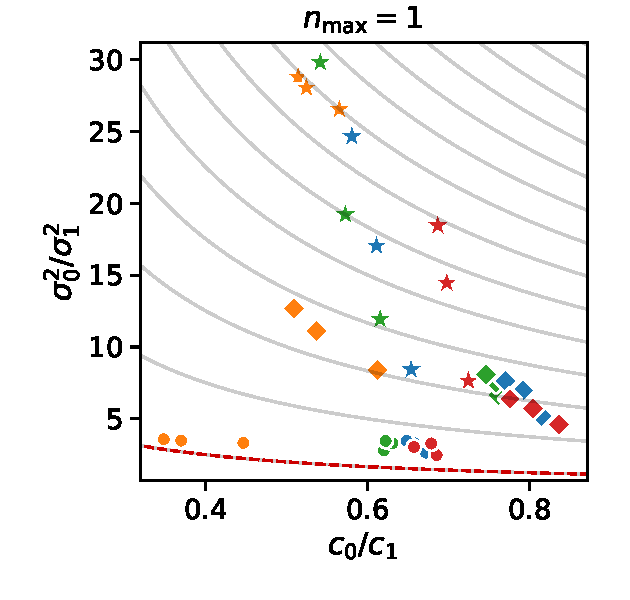
\includegraphics[scale=.5]{gfx/eff_landscape_order1.pdf}
    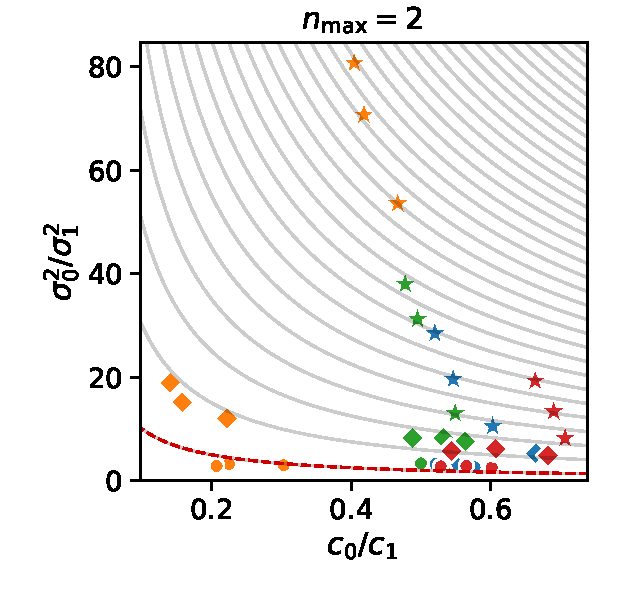
\includegraphics[scale=.5]{gfx/eff_landscape_order2.pdf}
    \end{minipage}
    \hfill
    \begin{minipage}{.4\textwidth}
	    \vfill
    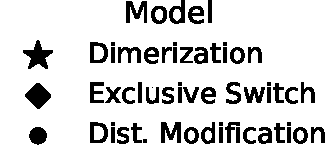
\includegraphics[scale=.5]{gfx/legend_models.pdf}
	    \vfill
    \end{minipage}
    \begin{minipage}{.4\textwidth}
	    \vfill
    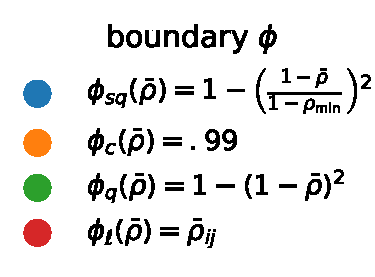
\includegraphics[scale=.5]{gfx/legend_phi.pdf}
	    \vfill
    \end{minipage}
    \hfill
    \caption[Cost \& variance reduction trade-off]{A visualisation of the trade-off between variance reduction $\sigma_0^2/\sigma_1^2$
    and cost ratio $c_0/c_1$. Isolines for efficiencies are given in grey. The break-even
    is marked by the dashed red line.
    Markers of the same kind differ in $n_{\lambda}$ and shift with increasing value
    upwards in variance reduction and lower in $c_0/c_1$, i.e.\ the shift is to the left and upwards
    with increasing $n_{\lambda}$.
	The sample size was $n=\num{10000}$ in all cases
    with $d=100$. Furthermore, $k_{\min}=3$ and $\pi_\lambda=N(0,1)$.}
    \label{fig:trade_off}
\end{figure}

We also observe, that an increase of $n_{\lambda}$ is particularly beneficial, if
the sampling distribution $\pi_{\lambda}$ does not capture the parameter region of
the highest correlations well.
This can be seen for the Dimerization case study, where the variance reduction increases
strongly with increasing sample size (\autoref{fig:efficiencies_alg_params}, \autoref{tab:eff1}, \autoref{tab:eff2}, \autoref{tab:eff3}).
Since $\pi_{\lambda}=N(0,1)$, more samples are needed to sample efficient $\lambda$-values (cf.\ \autoref{fig:bdim}).

In \autoref{fig:efficiencies_alg_params} we give detailed information on the influence of
algorithm parameters $k_{\min}$, the number of initial $\lambda$ values, and
different redundancy rules.
The $\lambda$ sampling distribution $\pi_{\lambda}$ is a standard normal.

Finally, we discuss the effect of the sample size $n$ on the efficiency $E$. In \autoref{fig:sample_sizes}
we give both the efficiencies and the slowdown for different sample sizes.
As a redundancy rule we used the unscaled quadratic function, $30$ initial values of $\lambda$,
and $k_{\min}=3$. With increasing sample size, the efficiency usually approaches an upper limit.
This is due to the fact that most control  variates are dropped early on and
the control  variates often remain the same for the rest of the simulations.
If we assume there are no helpful control  variates in the initial set
and all would be removed at iteration $100$, the efficiency would converge to $1$
for $n\to \infty$.
\begin{figure}[htb]
	\myfloatalign
	\subfloat[Efficiency v.\ sample size]
	{\label{fig:sample_sizes:eff}
	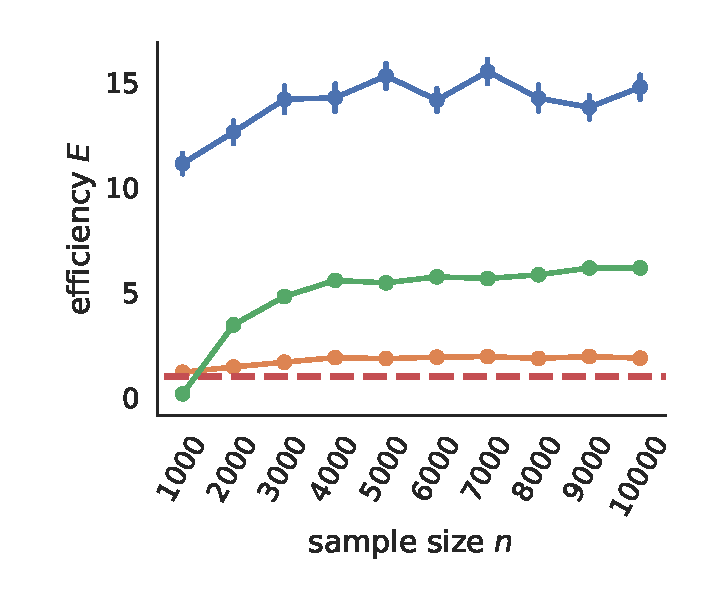
\includegraphics[scale=.38]{gfx/sample_size_efficiency.pdf}}\quad
	\subfloat[Slowdown v.\ sample size]
	{\label{fig:sample_sizes:slowdown}
	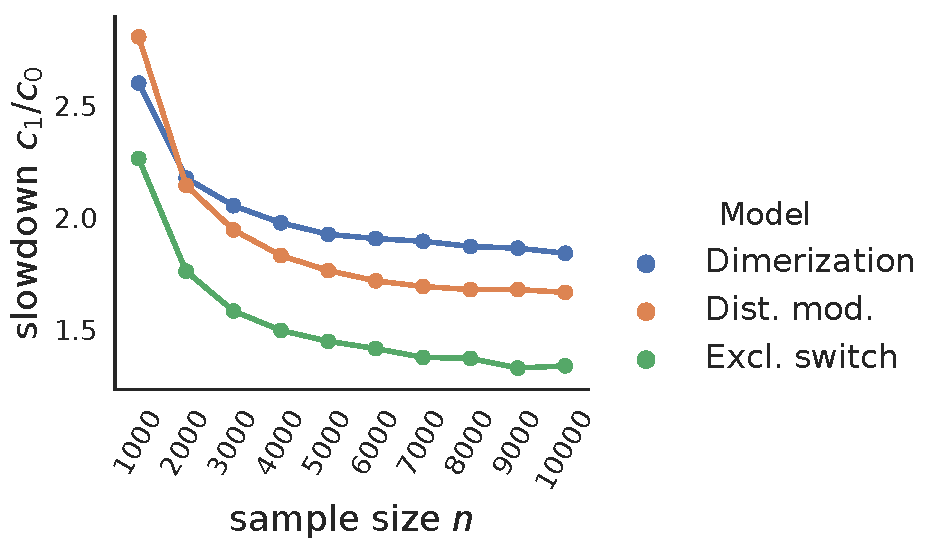
\includegraphics[scale=.38]{gfx/sample_size_slowdown.pdf}}
	\caption[Effect of sample size on control variate performance]{
    The effect of sample size on the efficiency $E$ and slowdown in the different case studies.
    The break-even $E=1$ is marked by the dashed red line.
    The cost increase due to the variance reduction over different sample sizes.}
    \label{fig:sample_sizes}
\end{figure}

%%%%%%%%%%%%%%%%%%%%%%%%%%%%%%%%%%%%%%%%%%%%%%%%%%
% Festschrift material %%%%%%%%%%%%%%%%%%%%%%%%%%%
%%%%%%%%%%%%%%%%%%%%%%%%%%%%%%%%%%%%%%%%%%%%%%%%%%
\section{Resampling Algorithm}\label{sec:splitting}
In previous work \parencite{backenkohler2019control}, we have proposed an algorithm that learns a set of
control variates through refinement of an initial set.
This initial set of control variates is based on samples of the time-weighting $\lambda$.
Each control variate is then checked for effectiveness in isolation.
Furthermore the set is refined by considering variable pairwise to determine redundancies.

In this work, we improve on the initial selection of control variates.
The initial set of control variates is build using a splitting approach akin to sequential Monte Carlo methods:
Over multiple rounds, new control variates are samples based on performance in prior rounds.
That way, a set of variates is build up.
This set is then refined in a greedy manner, taking into account the correlation between variates.
This algorithm has the main benefit of needing less sensitive to user input.
In particular, no heuristic redundancy threshold has to be fixed, making this approach more flexible.

As we have seen in the previous section, effective control variates have a high correlation
with the target random variable.
In the case of a single variate, the variance reduction is directly proportional to $1-\rho^2$, where
$\rho$ is the correlation.
In our case, infinitely many choices of $Z$ are available.
Our goal is to choose a subset that
satisfies two objectives:
Firstly, every selected control variate should reduce the estimator's variance.
Secondly, the subset should not be too large, i.e.  we want to avoid redundancies to achieve 
 a good  overall computational efficiency of the variance reduction.


%Accordingly, we define an \emph{efficiency} value to estimate
%whether the reduction in variance is compensating for the associated cost increase.
%A natural baseline of any variance reduction is that it outweighs its associated additional costs.
%Let $\sigma_Y^2$ be the variance of $Y$.
% https://statweb.stanford.edu/~owen/mc/Ch-var-basic.pdf
% Then the variance of the mean, based on $n$ iid.\ samples is $\sigma_Y^2/n$.
% If we let $c_0$ be the cost (i.e.\ CPU time) of a single simulation run, the overall cost to
% achieve this variance is $nc_0$.
% To achieve a variance $\tau^2$, $\sigma_Y^2/\tau^2$ samples are necessary at a cost of
% $c_0\sigma_Y^2/\tau^2$. We can analogously argue for the CV estimate where the
% cost of a single iteration is $c_1$.
%The \emph{efficiency} of the method is the ratio of the necessary
%cost to achieve a similar reduction with the CV estimate $Y_{\text{CV}}$ compared to
%the standard estimate $Y$~\parencite{l1994efficiency,mcbook}, i.e.
%\begin{equation}
%E=\frac{c_0\sigma_Y^2}{c_1\sigma^2_{Y_{\text{CV}}}}\,.
%\end{equation}
%The cost ratio $c_0/c_1$ depends on both the specific implementation and the technical setup.
%The cost increase is  mainly due to the computation of the integrals in \eqref{eq:dis_int}.
%The accumulation over the trajectory directly increases the cost of a single simulation,
%which is the critical part of the estimation.

If the computation of a variate does not adequately compensate for its computation
with variance reduction, we do not want to include it.
Balancing both objectives is challenging because control variates often correlate with each other.
Such correlations expose redundancy between different variates.
This also becomes clear, when considering that the overall variance reduction  depends on
the coefficient of multiple correlation.
% \vw{is multiple the right word here? }

Here we follow a resampling paradigm:
We start by building up a set of candidates using a particle splitting approach.
After each splitting step, we generate a small number of \ac{SSA} samples to estimate correlations.
Promising candidates are chosen based on the \emph{improvement} they provide and their time-weighting parameter $\lambda$ is resampled (see \autoref{fig:resampling}).
The main benefit of this bottom-up approach is its lower dependence on the initial sampling distribution of $\lambda$.
Moreover, the procedure spends less time evaluating unpromising candidates.
After   generating a set of control variates, the overall covariance matrix is estimated using stochastic simulations.
Using this information, we construct an efficient subset using a greedy scheme, taking into account the redundancies between control variates.
We discuss \autoref{alg:splitting:lcv} in more detail below.

\begin{figure}
    \centering
    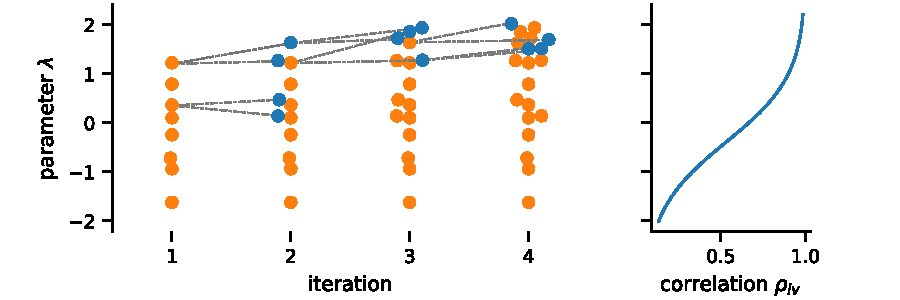
\includegraphics[scale=0.65]{gfx/resampling.pdf}
    \caption[Resampling algorithm]{An illustration of the resampling procedure for the time-weighting parameter $\lambda$ using \autoref{model:dm}. Areas giving higher correlations are resampled through multiple rounds. The newly sampled values are given in blue. In each round only the new candidates are evaluated.}
    \label{fig:resampling}
\end{figure}


\begin{algorithm}[ht]
\SetKwInOut{Input}{input}
\SetKwInOut{Output}{output}
\Input{$n, d, n_{\max}, n_{\lambda}, n_{c}, n_s, n_r$}
\Output{estimate using linear control variates}
  $L\leftarrow\{\lambda_i\sim \pi_\lambda \mid 1\leq i< n_{\lambda} \} \cup \{ 0 \}$\label{line:resampling:lambda_sample}\tcc*[r]{initialization}
  $P \leftarrow \{ ({m}, \lambda) | 1\leq\lvert {m} \rvert \leq n_{\max}, \lambda\in L\}$\label{line:resampling:init_covs}\;
  $P_{\text{all}} = \emptyset$
    \For{$i=1,\dots,n_r$\label{line:resampling:main_loop} \tcc*[r]{resampling}}{
        $(\hat{\Sigma},\hat{V}, \hat{Z}) \leftarrow \text{SSA}_{\text{CV}}(\pi_0,T,P,d)$\;

     $P_{\text{all}}\leftarrow P_{\text{all}}\cup P$\;
     $I_{\text{cands}}\leftarrow \{ k\sim \hat\gamma_{kv}/ \sum_{\ell}\hat{\gamma}_{\ell v} \mid 1\leq k \leq |P_{\text{all}}|, j=1,\dots,n_c\}$\label{line:resampling:resample}\;
     $P\leftarrow \bigcup_{k\in I_{\text{cands}}}\bigcup_{l=1}^{n_s}
     \{(m_k, \lambda_k') \mid \lambda_k'\sim N(\lambda_k, 0.5)\}$\label{line:resampling:end_resampling}\;
  	}
    $(\hat{\Sigma},\hat{V}, \hat{Z}) \leftarrow {\text{SSA}}_{\text{CV}}(\pi_0,T,P_{\text{all}},5d)$\label{line:resampling:search_loop}\tcc*[r]{covariance}
     $P^*=\emptyset$\;
     \While{$\exists i:
        (m_i, \lambda_i)\in P_{\text{all}}\setminus P^*\land$\\
        \hspace{4em}$\hat{\gamma}_{iv} \prod_{j=1;(m_j, \lambda_j)\notin P^*}^{\left|P_{\text{all}}\right|}
        \hat{\gamma}_{ij}^{-1}
        >\epsilon$\tcc*[r]{selection}\label{line:resampling:selection_loop}}{
        $k \leftarrow \argmax_i \hat{\gamma}_{iv}
        \prod_{j=1;(m_j, \lambda_j)\notin P^*}^{\left|P_{\text{all}}\right|}
        \hat{\gamma}_{ij}^{-1}$\label{line:resampling:selection}\;
        $P^*\leftarrow P^* \cup
            \{(m_k,\lambda_k)\}$\;
    }
    $(\hat{\Sigma},\hat{V}, \hat{Z}) \leftarrow \text{SSA}_{\text{CV}}(\pi_0,T,P^*,n)$\tcc*[r]{estimation}\label{line:resampling:sim}
    \Return $\hat{V} - {(\hat{\Sigma}_{{Z}}^{-1}\hat\Sigma_{{Z}V})}^{\top}\hat{{Z}}$\label{line:resampling:compute_lcv}
    \caption{\label{alg:splitting:lcv}Estimate the mean of species $i$ at time $T$}
\end{algorithm}

\paragraph{Initialization} A tuple $({m}_k, \lambda_k)$ of a moment vector ${m}_k$ and a time-weighting parameter $\lambda_k$
uniquely identifies a control variate $k$.
The algorithm starts out with an initial small set of control variates.
That is, we use $w(t)=e^{\lambda_kt}$ and $f(x)=x^{m_k}$ in \eqref{eq:poly_con}.
For a given set of time-weighting parameters $L$, we use all moments up to some fixed order $n_{\max}$ (\autoref{line:resampling:init_covs}).
For a fixed moment vector $m_k$ the time-weighting parameter $\lambda_k$ can lead to vastly different correlations $\rho_{kv}$ with the quantity of interest.
The best choices of $\lambda$ are usually not known beforehand.
Therefore, we sample an initial set of $\lambda$'s
from a fixed distribution $\pi_{\lambda}$ (\autoref{line:resampling:lambda_sample}).
Here, we use a standard normal distribution because its mean is the neutral weighting of $\lambda=0$ and extreme values are unlikely.

\paragraph{Resampling} Promising candidates are chosen from all control variates based on the estimated \emph{improvement ratio} they
provide, i.e.\ 
\begin{equation}
\hat{\gamma}_{kv} = ({1 - \hat{\rho}_{kv}^2})^{-1}
\end{equation}
following \eqref{eq:lcv_norm_varred}.
Specifically, control variate $k$ is chosen with probability proportional to
${\hat{\gamma}}_{kv}$ (\autoref{line:resampling:resample}).
The covariances of (only) the new variates are roughly estimated using very few (e.g., $d= 10$) \ac{SSA} samples. 
For the selected variates $I_{\text{cands}}$, the time-weighting parameter is resampled using a step distribution.
There is some freedom in the specifics of this resampling procedure.
In particular, the number of splits $n_c$ and descendants $n_s$ for each candidate control the number of additional candidates.
The algorithm performs $n_r$ rounds of resampling.
\autoref{fig:resampling} illustrates this part of the algorithm.

\paragraph{Covariance Estimation} After sampling a set of candidates this way, we need to select the most promising ones.
For this, we are interested in covariances between all control variates, as well.
Since the resampling does not provide us with such estimates, we evaluate all candidates together for a fixed number of simulations (\autoref{line:resampling:search_loop}).

\paragraph{Selection} The selection part of the algorithm (\autoref{line:resampling:selection_loop}) proceeds in a greedy fashion wrt.\ the potential estimated improvement $\hat{\gamma}_{iv}$ given by any variate.
However, covariates often have high mutual correlations.
For example, $Z_{\lambda}$ and $Z_{\lambda+\epsilon}$ for a small $\epsilon$ are typically highly correlated --- often more with each other than with the objective.
We want to avoid this unnecessary computational overhead from computing nearly redundant information and numerical problems due to the covariance matrix inversion (see \eqref{eq:lcv_asym}).
As a solution, we normalize the estimated improvement vector $(\hat{\gamma}_{iv})_i$ by
the product of the fractions of explained variances by the already selected covariates.
Therefore we choose the most promising candidate given a selection $P^{*}$ as
\begin{equation}
\argmax_{1\leq i \leq \left|P_{\text{all}}\right|}
\hat{\gamma}_{iv}
    \prod_{\substack{1\leq j\leq {\left|P_{\text{all}}\right|}\\(m_j, \lambda_j)\notin P^*}}
    \hat{\gamma}_{ij}^{-1}
\end{equation}
in \autoref{line:resampling:selection}.
This selection is done, until some lower threshold $\epsilon$ is reached (\autoref{line:resampling:selection_loop}).

\paragraph{Estimation} Finally, we simulate the model $n$ times (\autoref{line:resampling:sim}).
The resulting information enables an LCV estimation (\autoref{line:resampling:compute_lcv}).


We applied the presented algorithm for an estimation using $n=\num{10000}$ simulations.
Initially $n_{\lambda}=10$ samples for the time-weighting parameter were drawn from a standard normal distribution ($\pi_{\lambda} = N(0,1)$).
Constraints corresponding to each first-order moment, i.e.\ the process' expectations were generated ($n_{\max}=1$).
The covariance estimation during resampling used $d=10$ samples.

We evaluated the algorithm both with and without resampling for these first two case studies.
The algorithm without resampling  leaves out lines~\ref{line:resampling:main_loop}--\ref{line:resampling:end_resampling} from \autoref{alg:splitting:lcv}.
The evaluation without resampling provides a good point of comparison to our previous heuristics performance on these cases.
In the case of dimerization we observe a variance reduction of $\approx 27.67$ compared to a best case reduction of $\approx 28.75$ in our previous work.
This close performance however has to balance very different slowdown factors: With our new heuristic the slowdown is a factor of $\approx 1.34$ while in the previous case it was $\approx 1.95$.
Therefore the new method clearly outperforms in terms of efficiency ($\approx 20.5$ (new) versus $\approx 14.86$ (old)).
This is mainly due to the higher number of covariates used by the simple threshold heuristic.
In contrast the new method takes into account redundancies between covariances while still retaining good performance.
This becomes apparent when comparing the average number of used variates ($\approx 3.34$ (old) versus $\approx 1.98$ (new)).

The variance reduction factor for the distributive modification model is similar at $\approx 2.63$ (old) versus $\approx 2.66$ (new).
Noticeably, the new method uses on average fewer CVs ($\approx 2.74$) than the previous heuristic with the best efficiency ($\approx 3.23$).
The overall efficiency of the new algorithm with $1.72$ is slightly lower than the previous best value of $1.77$, due to a higher slowdown.
It is however important to note, that the trade-off differs significantly between different  heuristics used in the previous algorithm.
Furthermore, the lower average number of control variates would reduce the slowdown factor further, if more trajectories are generated.
% \paragraph{Filtering algorithm findings}
% \begin{itemize}
% \item results compared to prev work
%     \begin{itemize}
%     %     \item better for dimerization than previous work $(0.965224 1.945588 14.859417 3.338501)$
%     %     28.75546353807221 var red
%     %     1.945588 slodown
%     %      14.859417 efficiency (constant red)
%     %     versus 
%     % (1.3498338896993884, 27.6717070777087, 20.50008322421899)
%()
%     \item comparable for dist. mod (1.5462838232319676, 2.6620853997091847, 1.7216020498390927)
%     0.619560 1.488483 1.770218 3.232575
%     2.628535380086216 varred
%     \item much fewer LCV
%     \item Higher variance for lower correlations? (check this)
% \end{itemize}
% \end{itemize}
\begin{figure}[htb]
    \centering
    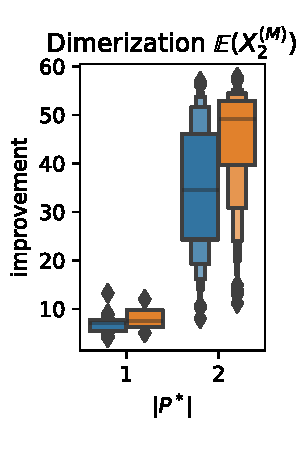
\includegraphics[scale=.65]{gfx/dim_improvement_numcv.pdf}
    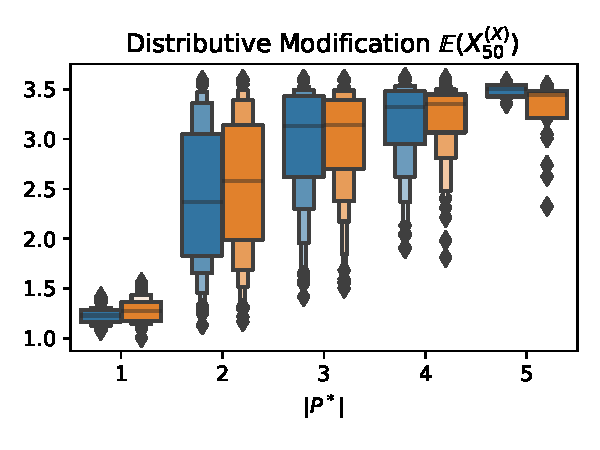
\includegraphics[scale=.65]{gfx/dm_improvement_numcv.pdf}
    
\includegraphics[scale=.65]{gfx/improvement_numcv_legend.pdf}
    \caption[Number of \ac{CV} v.\ variance reduction]{\label{fig:cv:refinement}The variance reduction factor $\sigma_{Y}^2 / \sigma_{Y_{LCV}}^2$ over different numbers of selected covariates with and without the resampling procedure.}
\end{figure}

In \autoref{fig:cv:refinement} we contrast the variance improvement ratio with and without the resampling algorithm. For the dimerization model, we see a clear improvement of variance reduction.
This improvement is due to the fact that the strongest correlations are present for $\lambda \approx 2.5$ (cf.\ \autoref{fig:resampling}).
This region of the time-weighting parameter space is less likely to be sampled by the initial
samples from the standard normal distribution.
Therefore the resampling procedure is especially beneficial if the better parameters $\lambda$ are farther from the origin.
In case of the distributive modification case study, we see a slight improvement.
Here, the best parameters $\lambda$ are close to zero and thereby more likely to be sampled by a standard normal.
Still, the resampling improves covariate performance for the most frequent cases of \num{2}--\num{4} covariates being selected (the case of \num{5} covariates has only a few instances).
Note, that the additional cost incurred by the resampling procedure is comparatively small, because
at most \num{4} candidates are evaluated in each iteration.
% \paragraph{SMC findings}
% \begin{itemize}
%     % \item The resampling makes finding better $Z$ more likely
%     \item resampling incurs a lower additional cost than a larger initial $L$ (because $|L| n_S^{n_{\max}}$
%     \item less reliance on $\pi_{\lambda}$
%     \item Figure \ref{fig:cv:refinement} discussion
%     \begin{itemize}
%         \item consistent improvement
%         \item most prominent with dimerization, because high correlations farther away from zero
%         \item $|P^*|=5$ and dist. mod. are few examples
%     \end{itemize}
% \end{itemize}


Next, we turn to the estimation of probabilities.
In particular, we consider the event of a species being below a threshold $\ell$ at time $t$ (species $M$ for the dimerization and $X$ for the distributive modification).
In \autoref{fig:thresholds} we summarize the results of this study for varying levels $\ell$.
In both case studies we observe that control variates are efficient for probabilities not close to either zero or one.
In this case control variates are able to reduce the variance of the estimated probabilities whilst maintaining a beneficial reduction-slowdown trade-off.
This region is larger for the distributive modification model because of its bimodal behavior.
If the probability to be estimated is close to either one or zero, the event occurs too rarely or too often, respectively, to adequately explain variance using linear correlations.
We note, that the worst case efficiency is close to one.
This is due to the algorithm throwing out all covariate candidates leaving us with a standard estimation.
Only the initial covariate evaluation and resampling causes a slowdown, driving efficiency slightly below one.
Naturally this cost decreases with more samples $n$.
\begin{figure}[htb]
    \centering
    
\includegraphics[scale=0.65]{gfx/legend_thres.pdf}\\
    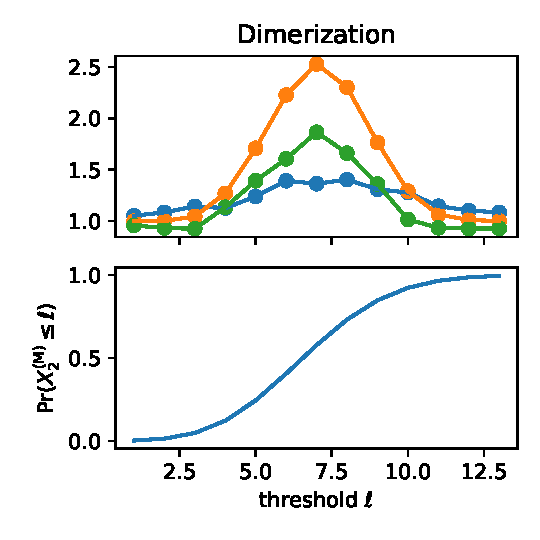
\includegraphics[width=.49\textwidth]{gfx/dim_thresholds.pdf}
    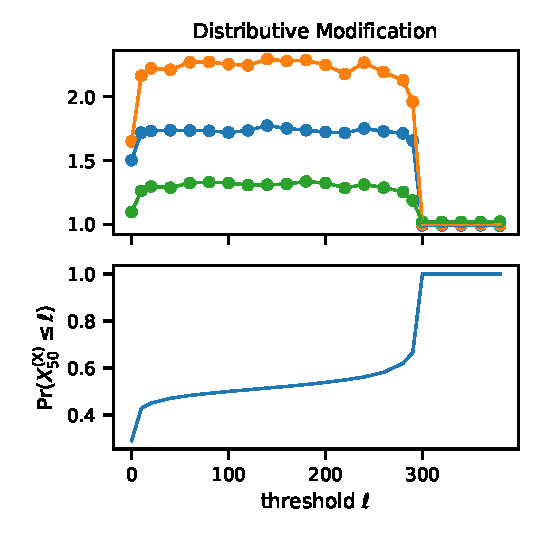
\includegraphics[width=.49\textwidth]{gfx/dm_threholds.pdf}
    \caption[\ac{CV} for probabililty estimation]{The methods efficiency for the estimation of threshold probabilities. For each threshold $\ell$ at least 200 estimations were performed.}
    \label{fig:thresholds}
\end{figure}

Control variates based on test functions restricted to intervals did not lead to an improvement (data not shown).

% \paragraph{Probability estimation}
% \begin{itemize}
%     \item LCV for Probabilities is most effective if probability is around .5
%     \begin{itemize}
%         \item Correlations can be more easily captured
%     \end{itemize}
%     \item LCV not effective for probs. close to 0 or 1
%     \item interval-based CVs do not perform better for threshold probabilities
% \end{itemize}


Finally, with the lac operon model we consider a larger case study. This model consists of \num{11} species and \num{25} --~partly non-linear~-- reactions.
\begin{model}[Lac operon]\label{model:lac}This is a well-known model of genetic regulation with positive feedback \parencite{stamatakis2009comparison}. Its reactions are
 \begin{gather*}
 \varnothing \xrightleftharpoons[k_19]{k_1} \mathrm{M_R}\,, \quad
 \mathrm{M_R} \xrightarrow{k_2} \mathrm{M_R + R}\,,\quad
 2 \mathrm{R} \xrightleftharpoons[k_4]{k_3} \mathrm{R_2}\,,\\
 \mathrm{R_2 + O} \xrightleftharpoons[k_6]{k_5}\mathrm{ R_2O}\,,\quad
 \mathrm{2 I + R_2} \xrightleftharpoons[k_8]{k_7} \mathrm{I_2R_2}\,,\\
\mathrm{2I +R_2O} \xrightleftharpoons[k_{10}]{k_9} \mathrm{I_2R_2 + O}\,,\quad
\mathrm{O}\xrightarrow{k_{11}} \mathrm{O + M_Y}\,,\\
\mathrm{R_2O}\xrightarrow{k_{12}}\mathrm{R_2O+M_Y}\,,\quad
\mathrm{M_Y} \xrightarrow{k_{13}}\mathrm{M_Y + Y}\,,\\
\mathrm{Y + I_{{ex}}}\xrightleftharpoons[k_{15}]{k_{14}}\mathrm{YI_{{ex}}}\,,\quad
\mathrm{YI_{{ex}}}\xrightarrow{k_{16}}\mathrm{Y+I}\,,\quad
\mathrm{I_{{ex}}}\xrightleftharpoons[k_{18}]{k_{17}}\mathrm{I}\,,\\
\mathrm{M_Y}\xrightarrow{k_{20}}\varnothing\,,\quad
\mathrm{R}\xrightarrow{k_{21}}\varnothing\,,\quad
\mathrm{R_2}\xrightarrow{k_{22}}\varnothing\,,\quad
\mathrm{Y}\xrightarrow{k_{23}}\varnothing\,,\\
\mathrm{YI_{ex}}\xrightarrow{k_{24}}\mathrm{I}\,,\quad
\mathrm{I_2R_2}\xrightarrow{k_{25}}\mathrm{2I}\,.\quad
\end{gather*}
Initially, $X^{(\mathrm{O})}_0=1$ and $X^{(\mathrm{I_{{ex}}})}=\num{48177}$ while all other abundancies are zero.
The parameters are $
  k_1  = 0.111$,
 $ k_2  = 15.0$,
  $k_3  = 103.8$,
  $k_4  = \num{0.001}$,
  $k_5  = 1992.7$,
  $k_6  = 2.4$,
  $k_7 =k_9  = \num{1.293d-7}$
  $k_8  = 12$,
  $k_{10} = 9963.2$,
  $k_{11} = 0.5$,
  $k_{12} = 0.01$,
  $k_{13} = 30.0$,
  $k_{14} = 0.249$,
  $k_{15} = 0.1$,
  $k_{16} = \num{6.0d4}$,
  $k_{17} =k_{18} = 0.92$,
  $k_{19} = k_{20} = 0.462$,
  $k_{21}=k_{22}= k_{23} = k_{24} = k_{25} = 0.2$.
\end{model}
We estimate the abundancy of LacY after one time unit, i.e.\ $\expSym(X^{(Y)}_1)$.
It is encoded by Y and facilitates
the lactose import via reactions \num{14} and \num{16}.
A typical simulation of the system up to time-horizon $T=1$ takes well above one minute of computational time.
Therefore we reduce the number of used trajectories to $n=1000$.
The other settings remain as above.

Despite the high dimensionality, we observe a good efficiency value of $E\approx 4.85$.
The slowdown caused by the method is approximately \num{1.98}.
A big part of this slowdown is due to the initial search of covariates.
Initially \num{10} covariates are generated for each first order moment, i.e.\ each of the
11 species. The number of additionally resampled covariates is similar to previous case studies.
Thus the main cost of the initial resampling and selection is due to the first iteration of the
resampling loop and the simulation loop of the selection procedure.
This part naturally has still potential for optimization:
Not all known covariates need to be reconsidered at the selection stage.
Instead, unpromising candidates could be discarded prior to that stage.

Still, the high variance reduction by a factor of approx.\ ${9.64}^{-1}$ more than compensates for this increase in computational cost, leading to the good overall efficiency.
This shows that, even for more complex models, the method is applicable and can extremely beneficial for Monte Carlo estimation.
% \begin{itemize}
%     \item For larger models such as this one, the up front cost of evaluating too many initial $\lambda$s is exacerbated.
%     \item 11 species 25 reactions
%     \item expensive simulations
% \end{itemize}
% \paragraph{Scalability findings}
% \begin{itemize}
% \item Setting:\begin{itemize}
%     \item $\expSym(X^{(Y)}_1)$
%     \item \num{1000} SSA runs
%     \item settings as above
% \end{itemize}
%     \item System size (dimensionality in particular; 11 species) do not harm the algorithm; especially despite blowup of initial constraints
%     \item Implementation and setup may be worth it even more in such expensive-to-simulate models
%     \item Highlight how long one simulation takes
%     \item slowdown: 1.9845426838974896
%     \item variance reduction: 9.640543124900878
%     \item efficiency: 4.857815960888073)
% \end{itemize}

\section{Conclusion}\label{sec:cv:conclusion}
In the context of Monte Carlo simulation, variance reduction
techniques offer an elegant way of improving the performance without
introducing approximation errors in addition to the statistical uncertainty.
In this work we have shown that known constraints on the moment dynamics can be successfully
leveraged in simulation-based estimation of expected values.
The empirical results indicate that
the supplementing a standard \ac{SSA} estimation with moment information
can drastically reduce the estimators' variance.
This reduction is paid for by accumulating information on the trajectory
during simulation.
However, the reduction is able to compensate for this increase.
This means that for fixed costs, using   estimates with
  control variates is more beneficial than using estimates without control variates.


In particular, we improve an initial subset by selecting particularly effective variates and removing redundant variates.
By resampling the time-weighting parameter $\lambda$ we ensure that appropriate values  are
flexibly explored.
In the worst case, all variates are dropped and the performance approaches the standard \ac{SSA}.
In most cases, however, a suitable subset is found together with the corresponding choices of $\lambda$.

We  analyze the performance of the method when estimating event probabilities and not only average molecule counts. Our largest case study has \num{11} species and
\num{24} reactions. %We achieve efficiencies of around \vw{say here what typical efficiencies are ; 2-4? Ist ja nicht viel ...}.

Another open question regarding this work is its performance when multiple
quantities instead of a single quantity are to be estimated. In such
a case, constraints would be particularly beneficial, if they lead
to improvements  as many estimation targets as possible.


In the future, we will further explore the algorithmic design space.
For example, the resampling distribution could be adjusted using decaying standard deviations.
Furthermore, we will look at different test functions weighting the state space more flexibly.
Different choices of $f$ and $w$ in \eqref{eq:poly_con} may improve 
efficiency further.
These choices become particularly interesting when moving from the estimation
of simple first order moments to more complex queries such as behavioural probabilities
of trajectories.
In such cases, one might even attempt to find efficient control variate functions
using machine learning methods.

Another worthwhile direction is the combination of \ac{CV} with other Monte Carlo techniques.
In particular, importance sampling might benefit from this.
Control variates of the biased process could be used to improve estimation of the likelihood ratio.

%\begin{subappendices}
%\section{Detailed Results}
%Detailed results for \acl{CV} presented in \autoref{ch:cvinsrns} are given in \autoref{tab:eff1}, \autoref{tab:eff2}, and \autoref{tab:eff3}.
%Experimental results of aggregation for stationary distribution approximation presented in \autoref{ch:statagg} are given in \autoref{tab:par_bd} and \autoref{tab:excl_switch}.
%%\section{Linear Control Variates}
%\begin{table}[htb]
    %\centering
	%\resizebox{\textwidth}{!}{
%\begin{tabular}{l@{\hskip 12pt}l@{\hskip 12pt}l@{\hskip 12pt}r@{\hskip 12pt}r@{\hskip 12pt}r@{\hskip 12pt}r}
%\toprule
	%$n_{\max}$ &   $n_{\lambda}$ & $\phi$ & $1-\frac{\sigma_1^2}{\sigma_0^2}$ &  slowdown &  efficiency &$\lvert P\rvert$ \\\midrule
	%\num{1}& $10$ &$\phi_{sq}$ &  $0.807184$ &  $1.227471$ &    $4.239255$ &   $2.536479$ \\
            %&    &$\phi_{c}$ &  $0.880285$ &  $1.633530$ &    $5.135205$ &   $7.411732$ \\
            %&    &$\phi_{q}$ &  $0.849082$ &  $1.312416$ &    $5.067770$ &   $3.639250$ \\
            %&    & $\phi_{\ell}$ &  $0.783459$ &  $1.195821$ &    $3.874778$ &   $2.090101$ \\\cmidrule{2-7}
            %& $20$ &$\phi_{sq}$ &  $0.856593$ &  $1.263340$ &    $5.539683$ &   $2.206154$ \\
            %&    &$\phi_{c}$ &  $0.910480$ &  $1.864405$ &    $6.011256$ &   $9.441336$ \\
            %&    &$\phi_{q}$ &  $0.867987$ &  $1.317958$ &    $5.765884$ &   $3.140806$ \\
            %&    & $\phi_{\ell}$ &  $0.825518$ &  $1.243075$ &    $4.627662$ &   $1.981143$ \\\cmidrule{2-7}
            %& $30$ &$\phi_{sq}$ &  $0.869165$ &  $1.298893$ &    $5.905196$ &   $2.059415$ \\
            %&    &$\phi_{c}$ &  $0.921019$ &  $1.966191$ &    $6.461331$ &   $9.928998$ \\
            %&    &$\phi_{q}$ &  $0.876822$ &  $1.340409$ &    $6.079876$ &   $2.762449$ \\
            %&    & $\phi_{\ell}$ &  $0.843288$ &  $1.288925$ &    $4.968796$ &   $1.983174$ \\\midrule
	%\num{2} & $10$ &$\phi_{sq}$ &  $0.811956$ &  $1.505521$ &    $3.544783$ &   $2.323999$ \\
            %&    &$\phi_{c}$ &  $0.916866$ &  $4.507566$ &    $2.681363$ &  $21.692390$ \\
            %&    &$\phi_{q}$ &  $0.868874$ &  $1.776190$ &    $4.309354$ &   $4.739893$ \\
            %&    & $\phi_{\ell}$ &  $0.795802$ &  $1.466579$ &    $3.353046$ &   $2.016196$ \\\cmidrule{2-7}
            %& $20$ &$\phi_{sq}$ &  $0.832562$ &  $1.657484$ &    $3.617313$ &   $2.085711$ \\
            %&    &$\phi_{c}$ &  $0.934280$ &  $6.348223$ &    $2.406431$ &  $29.976320$ \\
            %&    &$\phi_{q}$ &  $0.878944$ &  $1.879341$ &    $4.416281$ &   $3.990881$ \\
            %&    & $\phi_{\ell}$ &  $0.837922$ &  $1.647329$ &    $3.759896$ &   $1.978017$ \\\cmidrule{2-7}
            %& $30$ &$\phi_{sq}$ &  $0.829427$ &  $1.844766$ &    $3.190308$ &   $2.043201$ \\
            %&    &$\phi_{c}$ &  $0.947324$ &  $7.130628$ &    $2.673225$ &  $32.513670$ \\
            %&    &$\phi_{q}$ &  $0.878830$ &  $2.053317$ &    $4.034987$ &   $3.611746$ \\
            %&    & $\phi_{\ell}$ &  $0.824936$ &  $1.838879$ &    $3.118728$ &   $1.978836$ \\
%\bottomrule
%\end{tabular}}
    %\caption[Variance reduction results for up to second order moments]{Variance reduction results for up to second order moments with parameters $n_{\max}=2$, $n=\num{10000}$, $d=100$, $k_{\min}=3$. Exclusive switch.}
    %\label{tab:eff1}
%\end{table}

%\begin{table}[htb]
    %\centering
	%\resizebox{\textwidth}{!}{
%\begin{tabular}{l@{\hskip 12pt}l@{\hskip 12pt}l@{\hskip 12pt}r@{\hskip 12pt}r@{\hskip 12pt}r@{\hskip 12pt}r}
%\toprule
	%$n_{\max}$ &   $n_{\lambda}$ & $\phi$ & $1-\frac{\sigma_1^2}{\sigma_0^2}$ &  slowdown &  efficiency &$\lvert P\rvert$ \\\midrule
%$1$ & $10$ &$\phi_{sq}$ &  $0.619560$ &  $1.488483$ &    $1.770218$ &   $3.232575$ \\
            %&    &$\phi_{c}$ &  $0.700255$ &  $2.241695$ &    $1.492171$ &   $8.008607$ \\
            %&    &$\phi_{q}$ &  $0.643550$ &  $1.613001$ &    $1.743500$ &   $3.817641$ \\
            %&    & $\phi_{\ell}$ &  $0.596650$ &  $1.459405$ &    $1.703170$ &   $2.657000$ \\\cmidrule{2-7}
            %& $20$ &$\phi_{sq}$ &  $0.697414$ &  $1.519425$ &    $2.181687$ &   $2.631677$ \\
            %&    &$\phi_{c}$ &  $0.713445$ &  $2.706546$ &    $1.292838$ &  $10.295856$ \\
            %&    &$\phi_{q}$ &  $0.697654$ &  $1.585313$ &    $2.092817$ &   $3.398235$ \\
            %&    & $\phi_{\ell}$ &  $0.695846$ &  $1.473976$ &    $2.235418$ &   $2.226530$ \\\cmidrule{2-7}
            %& $30$ &$\phi_{sq}$ &  $0.712941$ &  $1.543068$ &    $2.263644$ &   $2.378037$ \\
            %&    &$\phi_{c}$ &  $0.721354$ &  $2.874249$ &    $1.252541$ &  $10.910880$ \\
            %&    &$\phi_{q}$ &  $0.711877$ &  $1.607712$ &    $2.164485$ &   $2.979704$ \\
            %&    & $\phi_{\ell}$ &  $0.669963$ &  $1.522184$ &    $1.996300$ &   $2.085473$ \\\midrule
%$2$ & $10$ &$\phi_{sq}$ &  $0.619450$ &  $1.734737$ &    $1.519168$ &   $3.148184$ \\
            %&    &$\phi_{c}$ &  $0.665361$ &  $3.301159$ &    $0.909443$ &  $13.456259$ \\
            %&    &$\phi_{q}$ &  $0.680592$ &  $1.840457$ &    $1.705876$ &   $3.864240$ \\
            %&    &$\phi_{\ell}$ &  $0.612674$ &  $1.662962$ &    $1.556868$ &   $2.659592$ \\\cmidrule{2-7}
            %& $20$ &$\phi_{sq}$ &  $0.684789$ &  $1.811408$ &    $1.755652$ &   $2.687379$ \\
            %&    &$\phi_{c}$ &  $0.689835$ &  $4.455005$ &    $0.726640$ &  $17.609554$ \\
            %&    &$\phi_{q}$ &  $0.687665$ &  $1.901258$ &    $1.688449$ &   $3.413595$ \\
            %&    &$\phi_{\ell}$ &  $0.651262$ &  $1.770238$ &    $1.623924$ &   $2.266729$ \\\cmidrule{2-7}
            %& $30$ &$\phi_{sq}$ &  $0.690602$ &  $1.922217$ &    $1.686011$ &   $2.375455$ \\
            %&    &$\phi_{c}$ &  $0.649191$ &  $4.837419$ &    $0.591701$ &  $19.145054$ \\
            %&    &$\phi_{q}$ &  $0.701253$ &  $2.001179$ &    $1.677062$ &   $3.007525$ \\
            %&    &$\phi_{\ell}$ &  $0.639123$ &  $1.894074$ &    $1.467403$ &   $2.086275$ \\
%\bottomrule
%\end{tabular}}
    %\caption[Variance reduction results for up to second order moments]{Variance reduction results for up to second order moments with parameters $n_{\max}=2$, $n=\num{10000}$, $d=100$, $k_{\min}=3$. Distributive modification.}
    %\label{tab:eff2}
%\end{table}

%\begin{table}[htb]
    %\centering
%\begin{tabular}{l@{\hskip 12pt}l@{\hskip 12pt}l@{\hskip 12pt}r@{\hskip 12pt}r@{\hskip 12pt}r@{\hskip 12pt}r}
%\toprule
	%$n_{\max}$ &   $n_{\lambda}$ & $\phi$ & $1-\frac{\sigma_1^2}{\sigma_0^2}$ &  slowdown &  efficiency &$\lvert P\rvert$ \\\midrule
	%\num{1} & $10$ &$\phi_{sq}$ &  $0.881641$ &  $1.530137$ &    $5.558692$ &   $1.621917$ \\
            %&    &$\phi_{c}$ &  $0.965224$ &  $1.945588$ &   $14.859417$ &   $3.338501$ \\
            %&    &$\phi_{q}$ &  $0.916445$ &  $1.625232$ &    $7.409904$ &   $1.997045$ \\
            %&    & $\phi_{\ell}$ &  $0.868288$ &  $1.380344$ &    $5.529745$ &   $1.081152$ \\\cmidrule{2-7}
            %& $20$ &$\phi_{sq}$ &  $0.941153$ &  $1.637272$ &   $10.437978$ &   $1.842971$ \\
            %&    &$\phi_{c}$ &  $0.964204$ &  $1.907999$ &   $14.747328$ &   $2.915082$ \\
            %&    &$\phi_{q}$ &  $0.947984$ &  $1.747519$ &   $11.072422$ &   $2.227250$ \\
            %&    & $\phi_{\ell}$ &  $0.931030$ &  $1.433401$ &   $10.169570$ &   $1.088572$ \\\cmidrule{2-7}
            %& $30$ &$\phi_{sq}$ &  $0.959517$ &  $1.723449$ &   $14.404936$ &   $1.972426$ \\
            %&    &$\phi_{c}$ &  $0.962514$ &  $1.770936$ &   $15.142156$ &   $2.216103$ \\
            %&    &$\phi_{q}$ &  $0.966216$ &  $1.847441$ &   $16.117387$ &   $2.446661$ \\
            %&    & $\phi_{\ell}$ &  $0.945724$ &  $1.456432$ &   $12.710196$ &   $1.084188$ \\\midrule
	%\num{2} & $10$ &$\phi_{sq}$ &  $0.905254$ &  $1.659799$ &    $6.402491$ &   $2.388472$ \\
            %&    &$\phi_{c}$ &  $0.987526$ &  $2.474939$ &   $33.074955$ &   $6.501180$ \\
            %&    &$\phi_{q}$ &  $0.923063$ &  $1.822654$ &    $7.195544$ &   $3.179257$ \\
            %&    & $\phi_{\ell}$ &  $0.878232$ &  $1.415909$ &    $5.830248$ &   $1.092264$ \\\cmidrule{2-7}
            %& $20$ &$\phi_{sq}$ &  $0.949038$ &  $1.831995$ &   $10.797164$ &   $2.890898$ \\
            %&    &$\phi_{c}$ &  $0.985710$ &  $2.391457$ &   $29.704344$ &   $5.450299$ \\
            %&    &$\phi_{q}$ &  $0.968076$ &  $2.021487$ &   $15.662368$ &   $3.681229$ \\
            %&    & $\phi_{\ell}$ &  $0.925413$ &  $1.449386$ &    $9.298961$ &   $1.072761$ \\\cmidrule{2-7}
            %& $30$ &$\phi_{sq}$ &  $0.964855$ &  $1.924268$ &   $14.911787$ &   $3.026275$ \\
            %&    &$\phi_{c}$ &  $0.981507$ &  $2.144089$ &   $25.520987$ &   $4.179125$ \\
            %&    &$\phi_{q}$ &  $0.973902$ &  $2.095985$ &   $18.507746$ &   $3.685851$ \\
            %&    & $\phi_{\ell}$ &  $0.948349$ &  $1.507425$ &   $12.904707$ &   $1.074538$ \\
%\bottomrule
%\end{tabular}
    %\caption[Variance reduction results for up to second order moments]{Variance reduction results for up to second order moments with parameters $n_{\max}=2$, $n=\num{10000}$, $d=100$, $k_{\min}=3$. Dimerization.}
    %\label{tab:eff3}
%\end{table}

%\end{subappendices}





\ctparttext{
	We present a
	state-space lumping scheme that aggregates states in a grid structure.
	Approximations based on this lumping are used to iteratively refine relevant
	and
	truncate irrelevant parts of the state-space.
	This way, the algorithm learns a well-justified finite-state
	projection for different scenarios.
}
\part{Aggregation \textit{\&} Refinement}\label{pt:aggregation}
\cleardoublepage\chapter{State-Space Aggregation}\label{ch:lumping}
In this part, we propose a  method to identify a truncation that optimizes the trade-off between the size of the considered state-space and the approximation error due to the \acf{FSP}\turnto{sec:fsp}.
To this end, we start with a very coarse-grained model abstraction that we refine iteratively. 
The coarse-grained model is based on an grid-shaped aggregation (i.e.\ lumping) scheme that identifies a set of macro-states.
These macro-states can be used to compute an interim model solution that guides the refinement in the next step.
We perform refinements until the approximation arrives at the resolution of the original model (i.e.\ each macro-state has only one constituent) such that the aggregation introduces no approximation error.

\section{Macro-States}
A macro-state is a collection of micro-states (or simply states) treated as one state in the aggregated model, which can be seen as an abstraction of the original model.
The aggregation scheme defines a partitioning of the state-space.
We choose a scheme based on a grid structure. That is, each macro-state is a hypercube in $\mathbb{Z}_{\geq 0}^{n_S}$.

Hence, each macro-state $\bar{x}_i(\ell^{(i)},u^{(i)})$ (denoted by $\bar{x}_i$ for notational ease) can be identified using two vectors $\ell^{(i)}$
and $u^{(i)}$.
The vector $\ell^{(i)}$ gives the corner closest to the origin, while $u^{(i)}$
gives the corner farthest from the origin.
Formally,
\begin{equation}\label{eq:macro_state}
    \bar{x}_i = \bar{x}_i(\ell^{(i)},u^{(i)}) =  \{x\in\mathbb{N}^{n_S} \mid  \ell^{(i)}  \leq x  \leq u^{(i)} \},
\end{equation}
where '$\leq$' denotes element-wise comparison.

In order to solve the aggregated model, we need to define transition rates between macro-states.
Therefore, we assume that, given that the system is in a particular macro-state, all constituent states are equally likely (uniformity assumption).
This assumption is the reason why the aggregated model provides only a coarse-grained approximation. 

The uniformity assumption is a modeling choice yielding significant advantages.
Firstly, it eases the computation of the rates between macro-states and, therefore, makes a fast solution of the aggregated model possible.
Secondly, even though it induces an approximation error, it provides suitable guidance as uniformity assumption spreads out the probability mass conservatively.
Hence, it becomes less likely that regions of interest are disregarded.
Lastly, the uniformity assumption is theoretically well-founded, as it stems from the maximum entropy principle: 
In the absence of concrete knowledge about the probability distribution inside a macro-state, we assume the distribution with the highest uncertainty, i.e., the uniform distribution. 

\section{Construction}
The grid structure makes the computation of transition rates between macro-states particularly convenient and computationally simple.
Mass-action reaction rates can be given in a closed-form,
due to the Faulhaber formulae~\cite{knuth1993johann} and more complicated rate functions such as Hill-functions can often be handled as well by taking appropriate integrals (see \autoref{sec:bridging:hill_toggle}).

Suppose, we are interested in the transition rate from macro-state $\bar{x}_i$ to macro-state $\bar{x}_k$ according to reaction $j$.
Using the uniformity assumption, this is simply the mean rate of the states in $\bar{x}_i$ that go to $\bar{x}_k$ using $j$.
However, only a small subset of constituents in $\bar{x}_i$ are actually relevant for this transition.
Hence, we identify the subset of states of $\bar{x}_i$ that lie at the border to $\bar{x}_k$ and in such a way that applying reaction $j$ shifts them to a state in $\bar{x}_k$. Then, we sum up the corresponding rates of these states. Lastly, we normalize according to the number of states inside of $\bar{x}_i$.

It is easy to see that the relevant set of border states is itself an
interval-defined macro-state $\bar{x}_{i\xrightarrow{j}k}$.
To compute this macro-state
we can simply shift $\bar{x}_i$ by $v_j$, take the intersection
with $\bar{x}_k$ and project this set back.
Formally,
\begin{equation}\label{eq:transition_set}
    \bar{x}_{i\xrightarrow{j}k} = ((\bar{x}_i + v_j) \cap \bar{x}_k) - v_j\,,
\end{equation}
where the additions are applied element-wise to all states
making up the macro-states.
For ease of notation, we also define a general exit state
\begin{equation}\label{eq:outgoing_set}
    \bar{x}_{i\xrightarrow{j}} = ((\bar{x}_i + v_j) \setminus \bar{x}_i) - v_j.
\end{equation}
This state captures all micro-states inside $\bar{x}_i$ that can leave the state via reaction $j$.

A particularly convenient feature of the transition states is, that they also are macro-states.
That means, they also are specified by independent intervals in each dimension as in \eqref{eq:macro_state}.
This holds because all operations in both \eqref{eq:transition_set} and \eqref{eq:outgoing_set} preserve this structure.

\begin{example}
In \autoref{fig:macro_states}
\marginpar{\autoref{model:par_bd} on page~\pageref{model:par_bd} gives this structure.}
we give an example of two adjacent macro states and the
transition state from the left to the right via one reaction.
As such it illustrates the result of the computation given in \eqref{eq:transition_set}:
The left state is shifted along the reaction vector, intersected with the right macro-state, and finally shifted back.
\begin{figure}[htb]
	\centering
	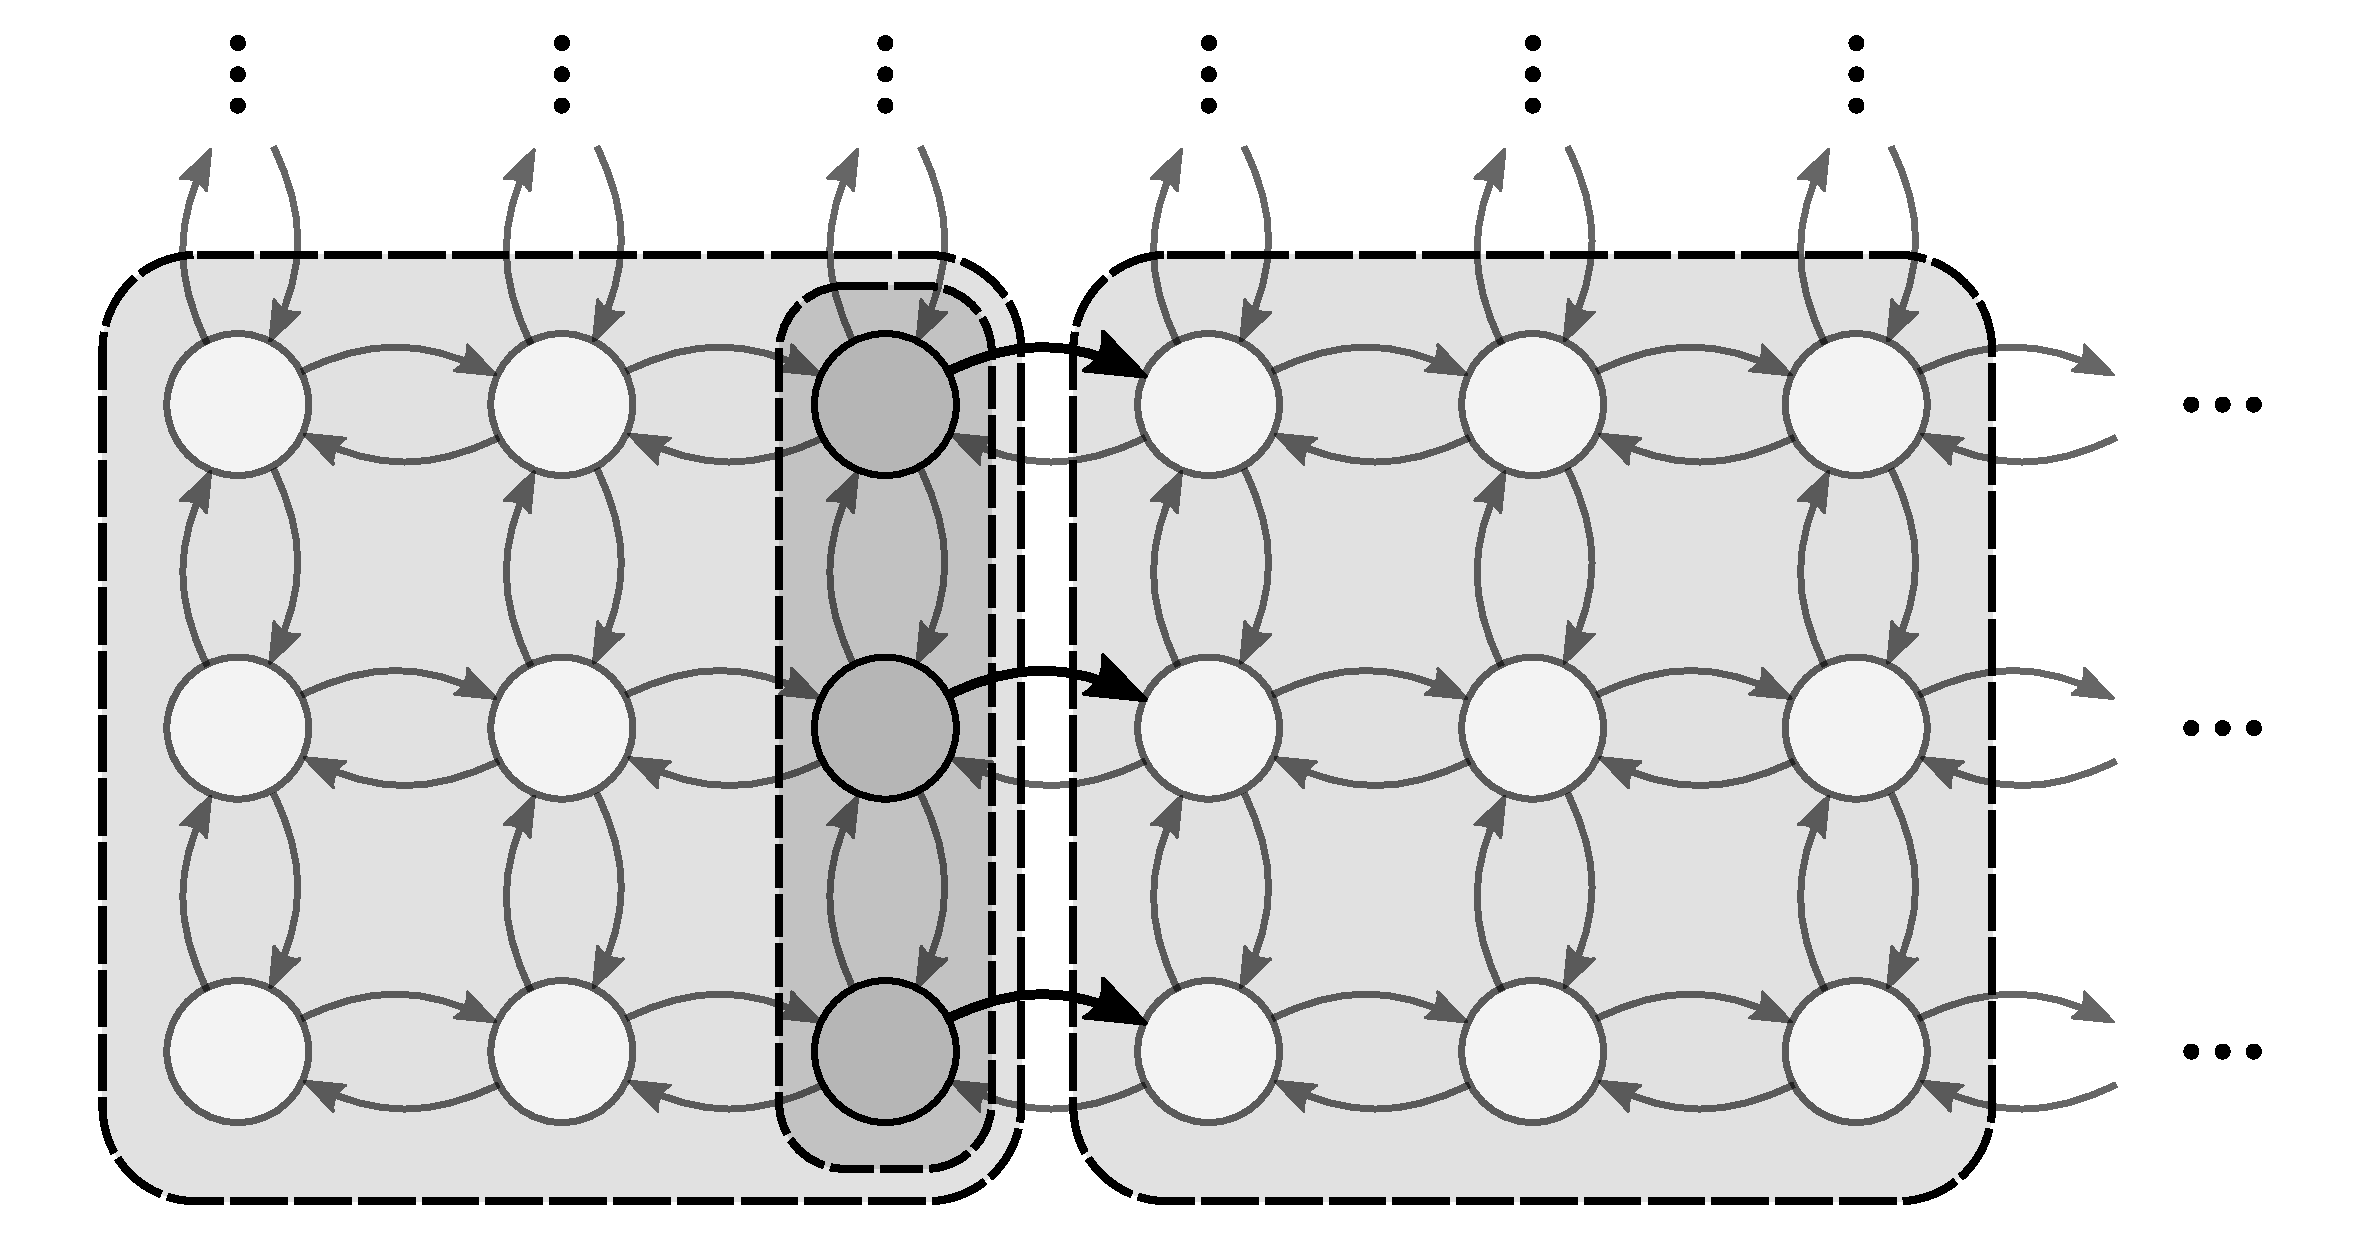
\includegraphics[width=0.9\textwidth]{gfx/macro_states.pdf}
	\caption[Macro-state transition]{\label{fig:macro_states}Two macro-states and a transition state from the left to the right.}
\end{figure}
\end{example}

This uniformity assumption gives rise to the following $Q$-matrix of the aggregated model:
\begin{equation}\label{eq:lumped_q}
    \bar{Q}_{ \bar{x}_i,  \bar{x}_k} = \begin{cases}
        \sum_{j=1}^{n_R}{\bar\alpha}_j\left(\bar{x}_{i\xrightarrow{j}k}\right)/\left|\bar{x}_i\right|\,,&\text{if}\; \bar{x}_i\neq \bar{x}_k\\[1ex]
        -\sum_{j=1}^{n_R}{\bar\alpha}_j\left(\bar{x}_{i\xrightarrow{j}}\right)/{\left|\bar{x}_i\right|}\,, &\text{otherwise}
    \end{cases}
\end{equation}
where 
\begin{equation}\label{eq:lumped_propfun}
    \bar{\alpha}_j({\bar{x}}) = \sum_{x\in \bar{x}} \alpha_j(x).
\end{equation}
is the sum of all rates belonging to reaction $j$ in $\bar{x}$.
In particular, the division by $\left|\bar{x}_i\right|$ in \eqref{eq:lumped_q} is due to the uniformity assumption: According to the assumption, given the process is in $\bar{x}_i$ it is in
each constituent micro-state of the transition state $\bar{x}_{i\xrightarrow{j} k}$ with probability $1/{\left|\bar{x}_i\right|}$.
Therefore, each of the added micro-state rates in \eqref{eq:lumped_propfun} is divided
by the state volume $\left|\bar{x}_i\right|$.

Under the assumption of polynomial rates, as is the case for mass-action
systems, we can compute the sum of rates over this transition set
efficiently using Faulhaber's formula.
\begin{example}
Consider the following mass-action reaction
$ 2 X \xrightarrow{c} \varnothing\,. $
For macro-state
$\bar{x} = \{0, \dots, n\}$
we can compute the corresponding lumped transition rate
\begin{align*}
	\bar{\alpha}(\bar{x})
	& =\frac{c}{2}\sum_{i=1}^n i (i - 1) 
	=\frac{c}{2}\left(\sum_{i=1}^n i^2 - \sum_{i=1}^ni\right)\\
	& =\frac{c}{2}\left(\frac{2n^3+3n^2+n}{6} - \frac{n^2 + n}{2}\right)
\end{align*}
eliminating the explicit summation in the lumped propensity function.
\end{example}

Interestingly, the lumped distribution
tends to be less concentrated. %\MB{rephrase this passage in terms of entropy?}\todo{L: this is interesting, but why? maybe an intuition of why uniform spreads more the distribution}
This is due to the assumption of a
uniform distribution inside macro-states.
This effect is illustrated by the example of a birth-death process below.
Due to this effect, an iterative refinement typically keeps an over-approximation in terms of state-space area.
This is a desirable feature since relevant regions are less likely to be pruned due to lumping approximations.

\begin{example}
We illustrate the scheme on the birth-death process, i.e.\ \autoref{model:bd}.
Its \ac{CTMC} has the following generator matrix
\[
	Q = \begin{bmatrix}
		-\mu & \mu & 0 & & & &\cdots \\
		\gamma & -(\mu + \gamma) & \mu & 0 & && \cdots\\
		0 & 2 \gamma & -(\mu + 2\gamma) & \mu & 0 && \cdots \\
		0 & 0 & 3\gamma & -(\mu + 3\gamma) & \mu &0&\cdots \\
		\vdots & \vdots & \vdots & \vdots & \vdots & \vdots&\ddots
	\end{bmatrix}
\]
The structure is more obvious in the graph visualization:
\vspace{2em}\\
\begin{tikzpicture}{thick}
	\node (n0) at (0, 0) [shape=circle, draw] {$0$};
	\node (n1) at (2, 0) [shape=circle, draw] {$1$};
	\node (n2) at (4, 0) [shape=circle, draw] {$2$};
	\node (n3) at (6, 0) [shape=circle, draw] {$3$};
	\node (n4) at (8, 0) [shape=circle, draw] {$4$};
	\node (n5) at (10, 0) {$\cdots$};
	
	\draw[->] (n0) edge[out=20, in=-200] node[above] {$\mu$} (n1);
	\draw[->] (n1) edge[out=20, in=-200] node[above] {$\mu$} (n2);
	\draw[->] (n2) edge[out=20, in=-200] node[above] {$\mu$} (n3);
	\draw[->] (n3) edge[out=20, in=-200] node[above] {$\mu$} (n4);
	\draw[->] (n4) edge[out=20, in=-200] node[above] {$\mu$} (n5);

	\draw[<-] (n0) edge[out=-20, in=-160] node[below] {$  \gamma$} (n1);
	\draw[<-] (n1) edge[out=-20, in=-160] node[below] {$2 \gamma$} (n2);
	\draw[<-] (n2) edge[out=-20, in=-160] node[below] {$3 \gamma$} (n3);
	\draw[<-] (n3) edge[out=-20, in=-160] node[below] {$4 \gamma$} (n4);
	\draw[<-] (n4) edge[out=-20, in=-160] (n5);
\end{tikzpicture}
\vspace{2em}\\
Now we lump states in groups of $5$ states.
	The states are constructed as\marginpar{We omit the vector notation here for clarity because the process has a single dimension.}
	\[
		\bar{x}_k(5k, (5+1)k - 1)
	\]
	The transition states for the birth reaction $\varnothing\rightarrow S$ is
	\[
		\bar{x}_{k\xrightarrow{1} k+1}=\{5(k+1) -1 \}\,.
	\]
	The lumped transition rate 
	\[
		\bar{\alpha}_1\left(\bar{x}_{k\xrightarrow{1} k+1}\right) = \mu\,.
	\]
	Similarly, the transition states for the death reaction $S\rightarrow \varnothing$ is
	\[
		\bar{x}_{k\xrightarrow{2} k+1}=\{5(k+1)\}\,.
	\]
	The lumped transition rate 
	\[
		\bar{\alpha}_2\left(\bar{x}_{k+1\xrightarrow{1} k}\right) = 5k\gamma\,.
	\]
	Using \eqref{eq:lumped_q} the aggregated transitions are as follows.
\vspace{2em}\\
\begin{tikzpicture}{thick}
	\node (n0) at (0, 0) [shape=circle, draw] {$[0,4]$};
	\node (n1) at (2, 0) [shape=circle, draw] {$[5,9]$};
	\node (n2) at (4, 0) [shape=circle, draw] {$[10,14]$};
	\node (n3) at (6, 0) [shape=circle, draw] {$[15,19]$};
	\node (n4) at (8, 0) [shape=circle, draw] {$[20,24]$};
	\node (n5) at (10, 0) {$\cdots$};
	
	\draw[->] (n0) edge[out=30, in=-210] node[above] {$\mu/5$} (n1);
	\draw[->] (n1) edge[out=30, in=-210] node[above] {$\mu/5$} (n2);
	\draw[->] (n2) edge[out=30, in=-210] node[above] {$\mu/5$} (n3);
	\draw[->] (n3) edge[out=30, in=-210] node[above] {$\mu/5$} (n4);
	\draw[->] (n4) edge[out=10, in=-200] node[above] {$\mu/5$} (n5);

	\draw[<-] (n0) edge[out=-30, in=-150] node[below] {$  \gamma$} (n1);
	\draw[<-] (n1) edge[out=-30, in=-150] node[below] {$2 \gamma$} (n2);
	\draw[<-] (n2) edge[out=-30, in=-150] node[below] {$3 \gamma$} (n3);
	\draw[<-] (n3) edge[out=-30, in=-150] node[below] {$4 \gamma$} (n4);
	\draw[<-] (n4) edge[out=-10, in=-160] (n5);
\end{tikzpicture}
In this example the rates remain in effect the same.
But the same number of macro-states covers more micro-states.

A forward integration\marginpar{The integration is done using an ad-hoc \ac{FSP} on $[0, 200]$.} of both, the model at original granularity and the aggregated version
is shown in \autoref{fig:lumped}.
\begin{figure}[htb]
    \centering
    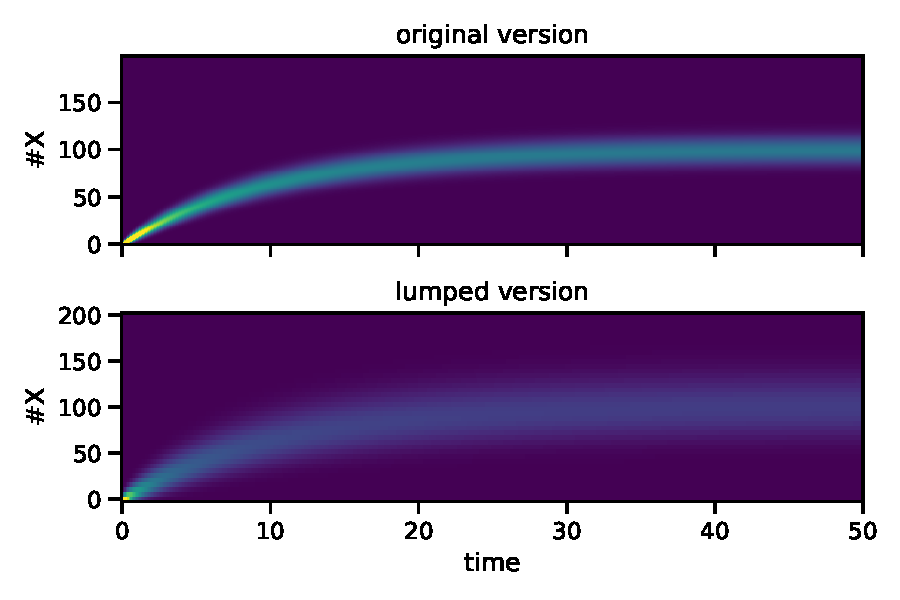
\includegraphics[scale=.6]{gfx/lumpedvorig.pdf}
	\caption[Lumping approximation of \autoref{model:bd}]{A lumping approximation of \autoref{model:bd} on the state-space truncation to $[0, 200]$ on $t\in[0, 50]$. On the left-hand side solutions of a regular truncation approximation and a lumped truncation (macro-state size is $5$) are given.}
    \label{fig:lumped}
\end{figure}
% \begin{figure}[htb]
%     \centering
%     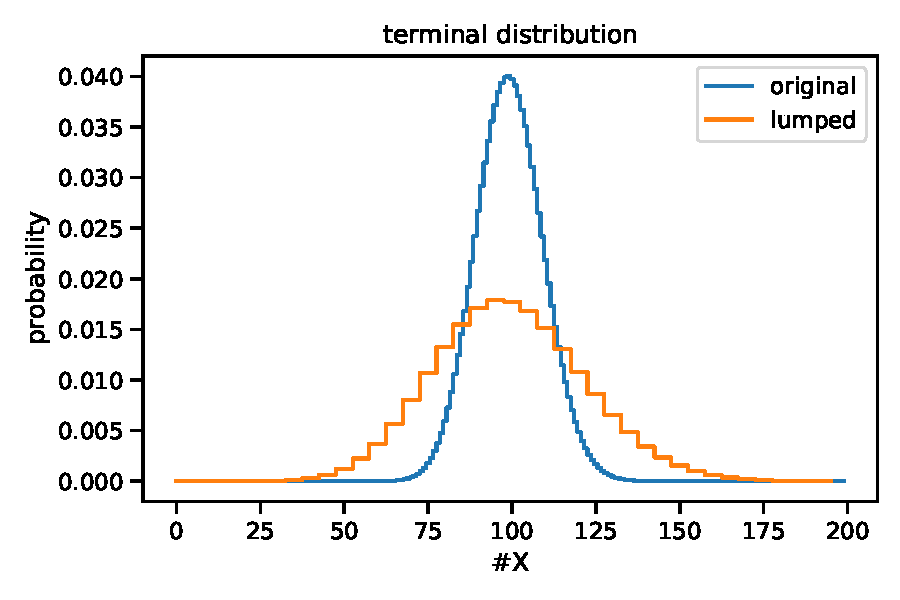
\includegraphics[scale=.6]{gfx/lumped_dist.pdf}
% 	\caption[Distribution of a lumped approximation]{The terminal distributions $\Pr(X_{50}=x_i)$ of a lumped approximation and a truncation at original granularity are given.}
%     \label{fig:lumped_terminal}
% \end{figure}
\end{example}

\section{Approximation Features}
Considering the previous example, we observe that the lumped version shows a similar temporal dynamic, but the distributions are spread out more.
This is a desirable feature because it indicates the location of the main probability mass with
significantly less states.

These features are not valid in general and the aggregation scheme remains a heuristic approach.
This is partly due to the \ac{MPM} formalism allowing for arbitrary propensity functions.
One can construct a process such that a significant change in dynamics inside a macro-state would be missed.
Mostly we encounter this phenomenon in models that exhibit a significant change near the zero-boundary for some species.
Examples include the toggle switch with Hill-functions (\autoref{model:hill_toggle}\turnto{model:hill_toggle}) and die-out in epidemics models (\autoref{model:seir}\turnto{model:seir}).
Other cases are rather rare in the standard model repertoire, but some awareness is necessary.

Fortunately, by refining the aggregation down to ``full resolution'', we can gain the guarantees inherent to \ac{FSP}.

\cleardoublepage\chapter{Truncations for Stationary Distributions}
An important part of the analysis of such models concerns their long-run behavior.
Given an ergodic underlying Markov chain, the chain's stationary distribution characterizes this behavior.
For some special model classes, such as zero-deficiency networks~\cite{anderson2011continuous}, analytical solutions for the stationary distribution are known.
However, most models require numerical approaches, often based on some form of approximation to guarantee tractability.
Those approaches can be based on stochastic simulation~\cite{gillespie1977exact} (which for steady-state analysis tends to be slow and inaccurate) or moment-bounds via mathematical programming~\cite{kuntz2017rigorous}.
Here, we draw on numerical approaches based on state-space truncation, which represent a viable option to approximate stationary distributions~\cite{kuntz2021approximations}.
Truncation-based approaches have the benefit of describing the complete dynamics within a finite subset of the typically very large or infinite state-space.
As such, they enable the approximation of complex distributions that are not well-described by low-order moments.

%Luca: up to here.

The main step in the computation of such an approximation is the identification of a suitable truncation,
i.e.\ a subset of the state-space encompassing most of the stationary probability mass.
Existing methods typically rely on Foster-Lyapunov drift conditions to define such subsets~\cite{dayar2011bounding}.
While these truncations come with bounds on the contained stationary probability mass, they typically are far larger than necessary.
The truncation is usually strongly constrained by the form of the chosen Lyapunov function~\cite{gupta2014scalable,dayar2011bounding}.
Optimizing over possible functions to identify efficient truncations is technically challenging and, to our knowledge, has not been demonstrated for general reaction networks~\cite{milias2014optimization}.

In this work, we address the identification of suitable truncations by using an aggregation-refinement scheme.
Initially, a Lyapunov analysis yields a set containing at least $1-\epsilon$ of the stationary probability mass.
On this subset of the state-space, we apply an aggregation scheme that groups together states in  hypercube macro-states.
Throughout each of these macro-states, we assume a uniform distribution among its constituent micro-states.
This allows us to roughly analyze large portions of the state-space with exponentially fewer variables.
We then iteratively truncate and refine the approximation based on the stationary distribution of this aggregated Markov chain. 
We keep only the most relevant macro-states and  continue this scheme until the macro-states contain a single original state. 
In this way, we arrive at an effective truncation to compute an approximation of the stationary distribution.

We investigate the approximation results on case studies with known stationary distributions and complex models with intricate stationary distributions.
We evaluate the truncation quality by assessing the stationary probability mass captured.
To this end, we use analytical solutions and bounds given by a Lyapunov analysis.
Further, we explore the control of the truncation size through the truncation parameter.
Finally, we demonstrate the method on the p53 oscillator model exhibiting a complex stationary distribution.


\section{Related Work}\label{sec:statagg:related}
For some specific models, analytical solutions for the stationary distribution have been found \cite{melykuti2014equilibrium,kurasov2018stochastic}. For the class of zero-deficiency networks, the stationary distribution is known to have a Poisson product form \cite{anderson2010product}. Monomolecular reaction networks can be solved explicitly, as well~\cite{jahnke2007solving}.

The analysis of countably infinite-sized state-spaces is often handled by pre-defined truncations~\cite{kwiatkowska2011prism}.
Sophisticated state-space truncations for the (uncon\-ditioned) forward analysis have been developed that give lower bounds.
They typically provide a trade-off between computational load and tightness of the bound~\cite{munsky2006finite,lapin2011shave,andreychenko2011parameter,henzinger2009sliding,mikeev2013fly}.
Such methods cannot be directly applied to the estimation of stationary distributions because the approximation usually introduces a sink-state.

Truncations for stationary distributions often involve re-direction schemes for transitions leaving and entering the subset.
A comprehensive survey of such state-space truncation methods can be found in \cite{kuntz2021stationary}.
A popular method of identifying truncations is the construction of a suitable Lyapunov function.
Beyond their use for establishing ergodicity \cite{meyn1993stability,gupta2014scalable,dayar2011bounding},
these functions can be used to obtain truncations, guaranteed to contain a certain amount of stationary probability mass \cite{dayar2011bounding}.
Using Lyapunov functions for the construction of truncations often leads to very conservative sets \cite{milias2014optimization}.
Different approaches have been employed to find truncations:
In \citet{gupta2017finite} \ac{SSA} estimates are used to set up an increasing family of truncations.

Apart from approaches based on state-space truncations, moment-based approaches have been particularly popular recently~\cite{ghusinga2017exact,dowdy2018bounds,kuntz2017rigorous,sakurai2017convex}.
Such approaches are based on the fact that particular matrices of distributional moments such as mean and variance are positive semi-definite.
Along with linear constraints stemming from the Kolmogorov equations \cite{backenkohler2016generalized}, a semi-definite program can be formulated and solved using existing tools.
While this method is suited to compute bounds on both moments and subsets of the state-space, its application is limited, due to numerical issues inherent in the formulation \cite{dowdy2018bounds}.

An approach where quantities are only described in terms of their magnitude has been proposed in \citet{ceska2019semi}. This allows for an efficient qualitative analysis of both dynamic and transient behavior.

An aggregation scheme similar to the one used here has been previously proposed in \citet{backenkohler2020analysis} to analyze the bridging problem on Markov population models.
This is the problem of analyzing process dynamics under both initial and terminal constraints.

Aggregation-based numerical methods for computing the stationary distribution 
of discrete or continuous-time Markov chains have been studied in
previous work. Popular approaches rely on an alternation of aggregation and 
disaggregation of the state-space \cite{stewart1994introduction,schweitzer1991survey}.
In the case of stiff chains, such aggregations are typically based on 
a separation of time-scales \cite{cao1985iterative}.
However, these methods have been developed for finite chains with arbitrary structure and are motivated by numerical issues of standard methods such as 
the power method or Jacobi iteration \cite{stewart1994introduction}.
They do not consider a truncation of irrelevant states, while
here our aggregation approach is used to determine the most relevant states
under stationary conditions in large or infinite chains with population structure.


\subsection{Stationary Distribution}\label{sec:statagg:stationary_dist}
Assuming
% irreducibility and 
ergodicity  
of the underlying chain, a stationary distribution $\pi_{\infty}$ is an invariant distribution, namely a fixed point of the Kolmogorov forward equation \eqref{eq:forward}.
Let $\pi_{\infty}$ be the vector description of a stationary distribution. It then  satisfies
\begin{equation}\label{eq:stationary}
0=\pi_{\infty}Q\quad\text{and}\quad 1=\sum_{x\in\mathcal{S}}\pi_{\infty}(x)
\end{equation}
as a fixed point of the Kolmogorov equation \eqref{eq:forward}.
Stationary distributions are connected to the \emph{long-run} behavior of an \ac{MPM}~\cite{dayar2011bounding}, as the system's distribution will converge to the (unique)
stationary distribution.
The connection of the stationary distribution to the long-run behavior becomes clear when considering the ergodic theorem. 
For some $A\subseteq\mathcal{S}$,
\begin{equation}\label{eq:ergodic}
    \lim_{T\to\infty}\frac{1}{T}\int_0^T 1_A(X_t)\,dt
    = \sum_{x\in A}\pi_{\infty}(x)\,.
\end{equation}
Thus, the mean occupation time for set $A$ over infinite trajectories is the stationary measure for $A$.
Eq.~\eqref{eq:ergodic} shows that we can assess long-run behavior using the stationary distribution and vice-versa.

\paragraph{Example.} Returning to the example of \autoref{model:bd} it is obvious that the state-space is irreducible.
Further, we can easily show, that the stationary distribution is Poissonian with rate $\mu/\gamma$:
$$ \pi_{\infty}(x)=\frac{{(\mu/\gamma)}^{x}\exp(-\mu/\gamma)}{x!}\,.$$


For simplicity, we assume throughout that the state-space is composed of a single communicating class.
Checking ergodicity given a countably infinite number of states is achieved by providing a suitable Foster-Lyapunov function \cite{meyn2012markov}.
Some automated techniques have been proposed for this task \cite{dayar2011bounding,gupta2014scalable,milias2014optimization}.



\subsection{Truncation-Based Approximation of $\pi_{\infty}$}\label{sec:statagg:fsp}
In many relevant cases, the state-space is huge or infinite and therefore the stationary solution cannot be computed directly.
To make such a computation possible we have to restrict ourselves to a finite manageable subset of the state-space and assume the majority of the probability mass is concentrated within that finite subset.
The main problem is to deal with the transitions leading to and from the truncated set (cf.\ \autoref{fig:truncation}).
In forward analysis, the outgoing transitions are simply redirected into a sink-state.
This way, a forward analysis provides lower bounds since mass leaving the truncation does not re-enter.
This approach, however, is unsuitable for the computation of stationary distributions because mass would accumulate in the sink-state leading to a distribution assigning all mass to it.
Therefore, transitions leaving the truncation need to be redirected back into the truncation.

The process' dynamics outside the truncation are defined by the \emph{stochastic complement} \cite{spieler2014numerical}.
If its behavior was known, one could redirect outgoing to incoming transitions optimally and preserve the correct stationary distribution.
However, this reentry distribution is typically unknown in most relevant cases.
Many different reentry distributions have been used, such as redirecting to some internal state or states with incoming transition from outside the truncation.
Reference~\cite{kuntz2021approximations} provides a comprehensive review of such methods.

The most natural choice is to pick a reentry distribution that redirects mass to states with incoming transitions from truncated states (cf.\ \autoref{fig:truncation} (center)).

Using varying redirections, we can compute bounds on the stationary probability conditioned on a truncation \cite[(Thm. 14)]{spieler2014numerical}.
To do this, one has to compute the stationary distribution for every possible way of connecting all outgoing to a single incoming transition.
Naturally, such an algorithm is rather expensive since one has to solve a linear system for each combination.
Therefore this method of computing bounds is costly on very large truncations, often given by Lyapunov functions.

When computing an approximation instead of bounds, we employ a uniform redirection scheme:
Outgoing transitions are split uniformly among incoming transitions.
Due to the threshold-based truncation scheme, we are likely to end up with a somewhat uniform distribution over in-boundary states (see \autoref{sec:statagg:alg}).


The identification of good truncations remains a major task in such approximations.
Using approaches such as Lyapunov functions (\autoref{sec:statagg:lyapunov}) \cite{dayar2011bounding} or moment-bounds \cite{kuntz2021approximations} can provide a good initial estimate, but typically the resulting truncations are far larger than necessary.
This leads to dramatically increased computational costs, especially when bounding methods mentioned above are performed.
Until a system for a larger truncation is solved, the precise location of  most of the probability mass is often unknown.
Instead of solving the full system for such a large space, we employ an aggregation scheme to cover large areas of the state-space with exponentially fewer variables.

Error bounds have been derived for increasing  truncation sets 
in the case of linear Lyapunov functions  \cite{gupta2017finite}.
However, until now it has not been shown that these bounds are applicable in practice \cite{meyn1994computable}.
Alternatively, one can monitor the product of the probability-ouflow rate and the maximum L1-norm, which bounds the approximation error up to a constant $M>0$, assuming a linear Lyapunov function exists \cite{gupta2017finite}.


\begin{figure}[t]
    \centering
    \begin{minipage}{0.6\textwidth}
    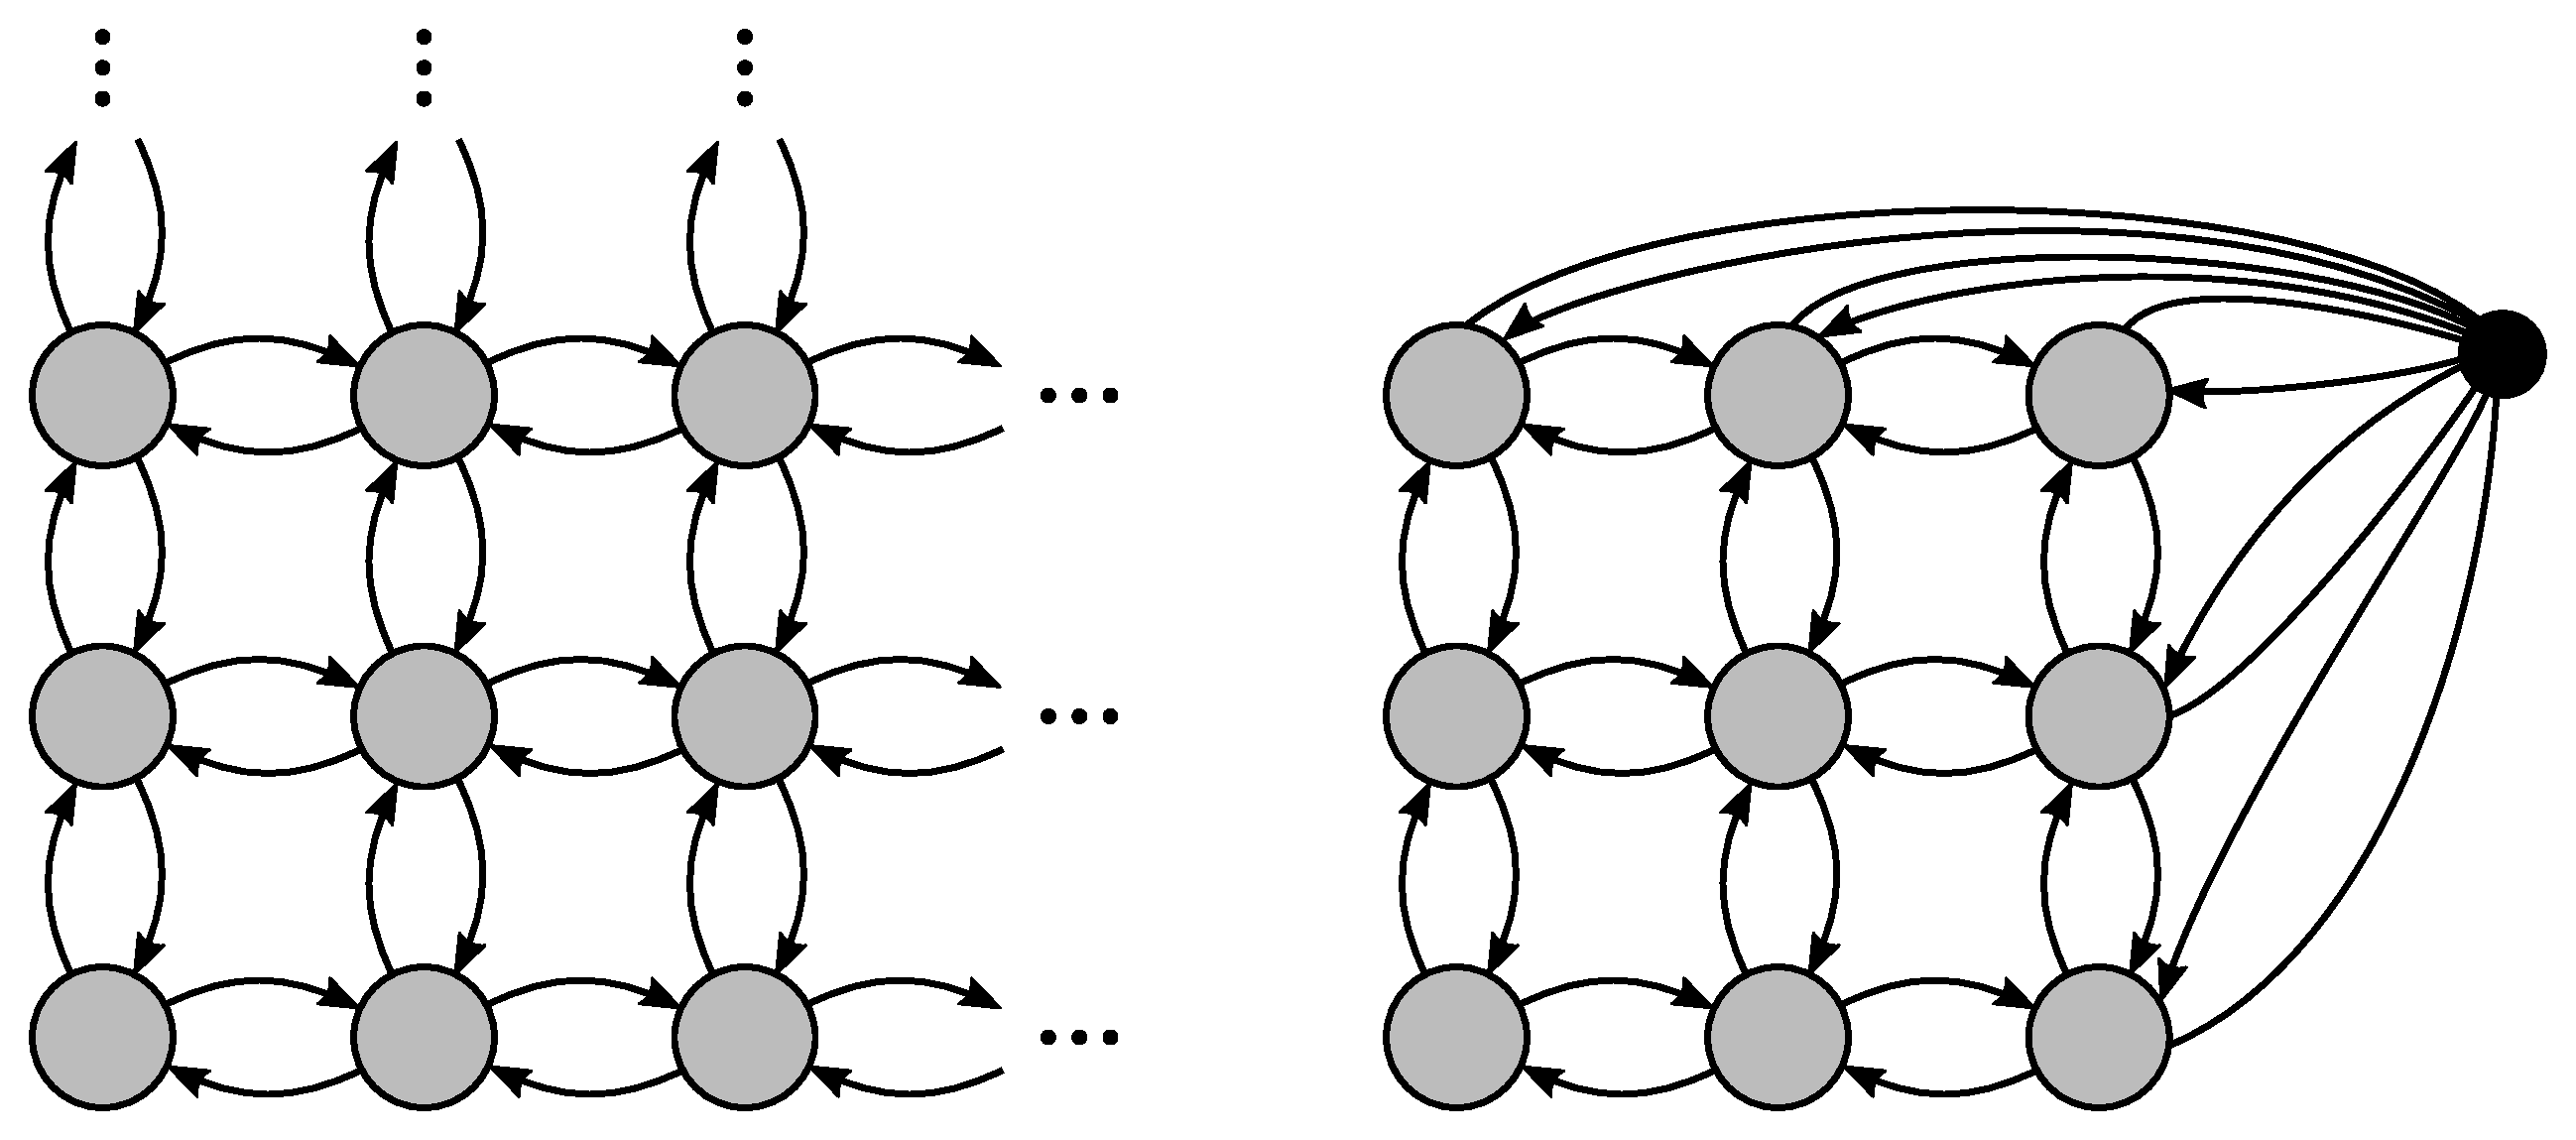
\includegraphics[width=\textwidth]{gfx/state_space_all.pdf}
    \end{minipage}
    \begin{minipage}{0.35\textwidth}
    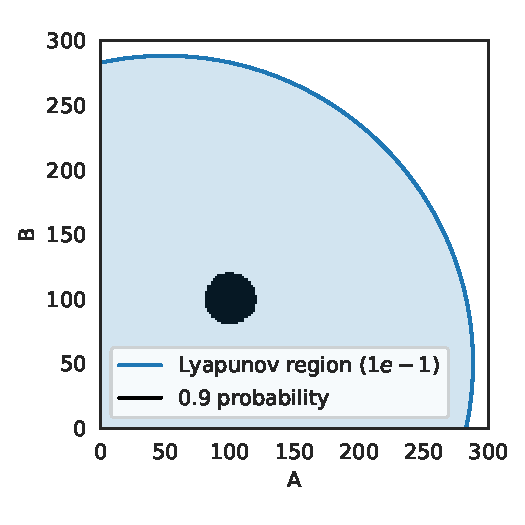
\includegraphics[width=\textwidth]{gfx/parbd_lya_v_truth.pdf}
    \end{minipage}
	\caption[\ac{FSP} for stationary distribution approximation]{(left) A countably infinite state-space. (center) Outgoing transitions are re-directed (according to the reentry distribution) to states that have incoming transitions from outside the truncation. (right) A comparison of the area prescribed by a Lyapunov analysis using Geobound and threshold 0.1 and the minimal area containing 0.9 stationary probability mass. The model is a parallel birth death process (\autoref{model:par_bd}).}
    \label{fig:truncation}
\end{figure}

\subsection{Lyapunov Bounds}\label{sec:statagg:lyapunov}
It is well-known that for a \ac{CTMC} $X$, ergodicity can be proven by a Lyapunov function $g:\mathcal{S}\to\mathbb{R}_+$ \cite{meyn1993stability,dayar2011bounding}.
Given the $g$, we define its \emph{drift} $d$ as its average infinitesimal change, which is obtained applying the generator $Q$ to $g$. 
\begin{equation}
    d(x) = \sum_{j=1}^{n_R} \alpha_j(x) (g(x+v_j) -  g(x))
\end{equation}
Usually, such a function $g$ grows in all directions on the positive orthant, while its drift $d(x)$ decreases in all directions.
More formally, $g$ is characterized by having finite level sets $\{x\in\mathcal{S} \mid g(x) < l\}$ for all $l > 0$.
At the same time,
\begin{equation}\label{eq:lyapunov_set}
    \mathcal{C}_{\epsilon_{\ell}} = \{ x\in\mathcal{S} \mid
    \frac{\epsilon_{\ell}}{c}d(x) > \epsilon_{\ell} - 1\}
\end{equation}
should be finite, where $\infty> c\geq \sup_{x\in\mathcal{S}} d(x)$.
In this case, $\mathcal{C}_{\epsilon_{\ell}}$ contains at least $1-\epsilon_{\ell}$ of stationary probability mass for any $\epsilon_{\ell}\in(0,1)$ \cite[Thm.~8]{spieler2014numerical}.
Given that $\mathcal{C}_{\epsilon_{\ell}}$ is finite, the chain is ergodic and
\begin{equation}
    \sum_{x\in\mathcal{C}_{\epsilon_{\ell}}}\pi(x)> 1 - \epsilon_{\ell}
\end{equation}
bounding the stationary probability mass contained within $\mathcal{C}_{\epsilon_{\ell}}$.

In many cases, simple choices of $g$ such as the L1- or L2- norm are sufficient.
However, the sets resulting from such functions are often very conservative.
Consider \autoref{fig:truncation} (right) as an example, where the Lyapunov truncation with $\epsilon_{\ell}=0.1$ %\vw{eps=0.1 sollte hier angegeben werden? }
for two parallel birth death processes (\autoref{model:par_bd}) is compared to the smallest set containing 0.9 of stationary probability.
Clearly, the area given by the Lyapunov function is magnitudes larger than necessary to capture probability mass consistent with $\epsilon_{\ell}$.

We employ this approach to both identify initial truncations and estimate errors in the evaluation.
Specifically, we employ the tool Geobound\marginpar{\url{https://mosi.uni-saarland.de/tools/geobound}} with L2-norm as function $g$ implementing techniques presented in \cite{dayar2011bounding}.

\section{Method}\label{sec:statagg:method}
In this work, we propose a  method to identify a truncation that optimizes the trade-off between the size of the considered state-space and the approximation error due to the \ac{FSP}.
To this end, we start with a very coarse-grained model abstraction that we refine iteratively. 
The coarse-grained model is based on an grid-shaped aggregation (i.e., lumping) scheme that identifies a set of macro-states.
These macro-states can be used to compute an interim model solution that guides the refinement in the next step.
We perform refinements until the approximation arrives at the resolution of the original model (i.e., each macro-state has only one constituent) such that the aggregation introduces no approximation error.

We explain the construction of macro-states in \autoref{sec:statagg:aggregation} and their initialization in \autoref{sec:statagg:initagg}.
We present the iterative refinement algorithm in \autoref{sec:statagg:alg}.



\subsection{Initial Aggregation}\label{sec:statagg:initagg}
The initial aggregated space $\hat{\mathcal{S}}^{(0)}$ should encompass all regions of the state-space that could contain significant mass because states outside this initial area will not be refined.
In principle, multiple approaches could be used to identify such a region.
One possibility is the computation of moment bounds for the stationary distribution~\cite{ghusinga2017exact,dowdy2018bounds}.
Based on these bounds on expectations and covariances, an initial truncation could be fixed.
The approach we use here is to identify such a  region by a Lyapunov analysis \cite{dayar2011bounding}.
This way, we obtain a polynomial describing a semi-algebraic subset of the entire state-space containing $1-\epsilon_{\ell}$ of the mass, where $\epsilon_{\ell}>0$ can be fixed arbitrarily.
These sets usually are far larger than a minimal set containing $1-\epsilon_{\ell}$ of stationary probability mass would be.
As an initial aggregation, we build an aggregation on a subset $[0..n]^{n_S}\subset \mathcal{S}$ containing the set prescribed by the Lyapunov analysis.


\subsection{Iterative Refinement Algorithm}\label{sec:statagg:alg}
\begin{figure}[t]
    \centering
    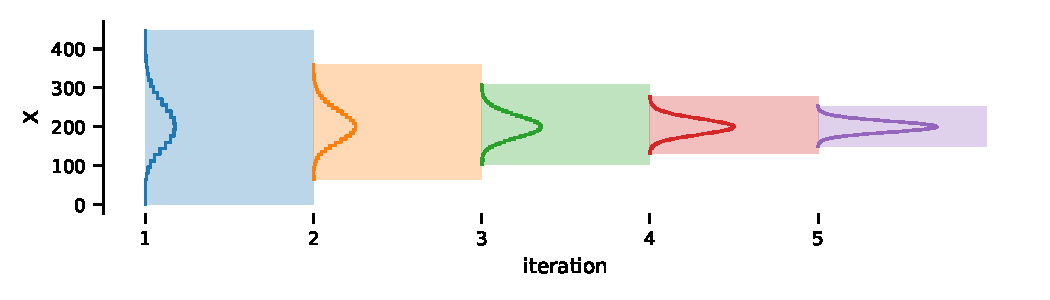
\includegraphics[width=\textwidth]{gfx/bd_truncs.pdf}
	\caption[State-space refinement algorithm for the stationary distribution]{The state-space refinement algorithm on a birth-death process. From left to right the state size is halved and states with low probability are removed from the truncation. The final truncation is a typical truncation with states of size 1 and the initial states are of size $2^4$.}
    \label{fig:refinement_alg}
\end{figure}


\begin{algorithm}
\SetKwFunction{Split}{split}
\SetKwInOut{Input}{input}
\SetKwInOut{Output}{output}
\Input{Initial partitioning $\mathcal{S}^{(0)}$, truncation threshold $\epsilon$}
\Output{approximate stationary distribution $\hat\pi_{\infty}$}
\For{$i=1,\dots,m$}{
    ${\hat\pi}^{(i)}_{\infty}\leftarrow $ solve approximate stationary distribution on $\mathcal{S}^{(i)}$\label{line:stationary}\;
    $\mathcal{R}\leftarrow$ choose smallest $\mathcal{R}'\subseteq\mathcal{S}^{(i)}$ such that $ \sum_{\bar{x}\in\mathcal{R}'}\hat{\pi}_{\infty}^{(i)}(\bar{x})\geq1-\epsilon$\label{line:filter}\;
    $\mathcal{S}^{(i+1)}\leftarrow \bigcup_{\bar{x}\in\mathcal{R}} \text{split}(\bar{x})$\label{line:refine:stat}\;
    update $\hat{Q}$-matrix\label{line:update_q:stat}\;
}
\Return ${\hat\pi}^{(m)}_{\infty}$\;
    \caption{Lumping to approximate the stationary distribution }
    \label{alg:refinement:stat}
\end{algorithm}
The refinement algorithm (\autoref{alg:refinement:stat}) starts with a set of large macro-states
that are iteratively refined, based on approximate stationary distributions.
We start by constructing square macro-states of size
$2^m$ in each dimension for some $m\in\mathbb{N}$ such that they form a large-scale grid $\mathcal{S}^{(0)}$. 
Hence, each initial macro-state has a volume of ${\left(2^m\right)}^{n_S}$.
This choice of grid size is convenient because we can halve states
in each dimension.
Moreover, this choice ensures that all states have an equal volume
and we end up with unit-sized macro-states,
equivalent to a truncation of the original non-lumped state-space.

An iteration of the state-space refinement starts by computing the stationary distribution, using the lumped $\hat Q$-matrix.
Based on a threshold parameter $\epsilon>0$
states are either removed or split (\autoref{line:refine:stat}), depending on
the mass assigned to them by the approximate stationary
probabilities $\hat\pi^{(i)}_{\infty}$.
Thus, each macro-state is either split into $2^{n_S}$ new states or removed
entirely.
The result forms the next lumped state-space $\mathcal{S}^{(i+1)}$.
The $\hat{Q}$-matrix is updated (\autoref{line:update_q:stat}) using \eqref{eq:lumped_q} to calculate the transition rates of the next aggregated truncation $\mathcal{S}^{(i+1)}$. 
Entries of truncated states are removed from the updated transition matrix.
Transitions leading to them are
re-directed according to the re-entry matrix (\autoref{sec:statagg:fsp}).
After $m$ iterations (we started with states of side lengths $2^m$)
we have a standard \ac{FSP} scheme
on the original model tailored to
computing an approximation of the stationary distribution.


This way, the refinement algorithm focuses only on those parts of the state-space contributing most to the stationary distribution.
For instance, in \autoref{fig:refinement_alg} the stationary probability mass mostly concentrates around $\#S=200$.
Therefore, states that are further away from this area can be dropped in further refinement.
This filtering (\autoref{line:filter} in \autoref{alg:refinement:stat}) ensures that
states contributing significantly to $\hat\pi_{\infty}^{(i)}$ will be kept and refined in the next iteration.
The selection of states is done by sorting states in descending order according to their approximate probability mass.
This ensures the construction of the smallest possible subset chosen for refinement according to the approximation.
Then states are collected until their overall approximate mass is above $1-\epsilon$.

An interesting feature of   the aggregation scheme is that the distribution
tends to spread out more.
This is due to the assumption of a uniform distribution inside macro-states.
To gain an intuition, consider a macro-state that encompasses a peak of the stationary distribution.
If we re-distribute the actual probability mass inside this macro-state uniformly,
a higher probability is assigned to states at the macro-state's border.
When plugging such macro-states together, this increased mass away from the peak will
increase the mass assigned to adjacent macro-states.
This effect is illustrated by the example of a birth-death process in \autoref{fig:refinement_alg}.
Due to this effect, an iterative refinement typically keeps an over-approximation in terms of state-space area.
This is a desirable feature since relevant regions are less likely to be pruned due to lumping approximations.

\section{Results}\label{sec:statagg:results}
A prototype was implemented in Rust~1.50 and Python~3.8.
The linear systems were solved either using Numpy~\cite{numpy} for up to 5000 states, or the sparse linear solver as available through Scipy~\cite{2020SciPy-NMeth}, or the iterative biconjugate gradient stabilized algorithm~\cite{van1992bi} (up to $10,\!000$ iterations and absolute tolerance $10^{-16}$).

The examples that we consider in the sequel 
are typical benchmarks for the analysis of \acp{MPM}. For most of them, appropriate Lyapunov functions
have been determined using Geobound \cite{spieler2014numerical}.
However, the corresponding Lyapunov sets containing at least $1-\epsilon_{\ell}$ of the stationary probability mass are very large for typical choices of $\epsilon_{\ell}$ (e.g. $\epsilon_{\ell}\in \{0.1,0.05,0.001\}$). Even
for extremely large $\epsilon_{\ell}$, say $\epsilon_{\ell}=0.8$, the remaining state-space may still be huge (e.g, 15,198 states).
\subsection{Parallel Birth-Death Process}
We first examine the algorithm on the simple example of two parallel, uncoupled birth-death processes.
\begin{model}[Parallel Birth-Death Process]\label{model:par_bd}
Two uncoupled parallel birth-death processes result in a simple stationary distribution that is
given by a product of two Poisson distributions.
$$\varnothing\xrightarrow{\rho} A \qquad A\xrightarrow{\delta} \varnothing \qquad
\varnothing\xrightarrow{\rho} B \qquad B\xrightarrow{\delta} \varnothing$$
As a parameterization we choose $\rho = 100$ and $\delta=1$.
\end{model}
For this model, the stationary distribution is known to be the product of two Poisson distributions with rate $\rho / \delta$.

According to the Lyapunov analysis with a 1e-4 bound, we fix the initial truncation to a $70\times 70$ grid of macro-states with size $2^7$ in each dimension.
This implies 8 iterations of the algorithm to arrive at a truncation with the original granularity.
In \autoref{fig:par_bd}, we illustrate the truncations of different iterations.
Over the iterations, the covered area decreases, while the aggregation granularity increases.
The final truncation distribution approximation is also depicted and covers $1 - \text{1.27e-2}$ of the true stationary distribution (cf.\ \autoref{tab:intervals}).

For this case study, we also compute state-wise bounds on the probabilities conditioned on the truncation as discussed in \autoref{sec:statagg:fsp}.
In \autoref{fig:par_bd_errors} (right), we present the difference between upper and lower bound for $\epsilon=0.1$.
We observe intervals that are narrowest in the truncation's interior near the distribution's mode.
The largest intervals or the largest absolute uncertainty is present in the boundary states.
This indicates, that the specific reentry distribution has little effect on the main approximate stationary mass.
More detailed results on the intervals' magnitudes are given in \autoref{tab:intervals}.
\begin{figure}[t]
    \centering
    \begin{minipage}{.48\textwidth}
    \centering
    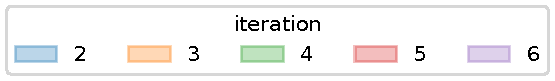
\includegraphics[scale=0.5]{gfx/iteration_legend.pdf}\\
    \vspace{-5mm}
    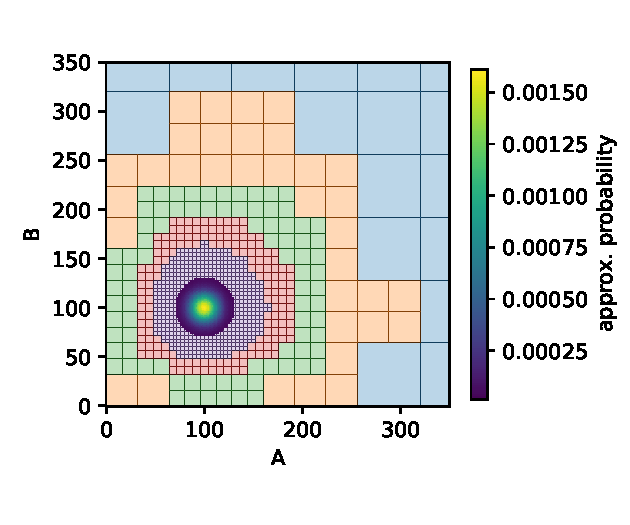
\includegraphics[width=\textwidth]{gfx/parbd_truncs.pdf}
    \end{minipage}
    \begin{minipage}{.43\textwidth}
    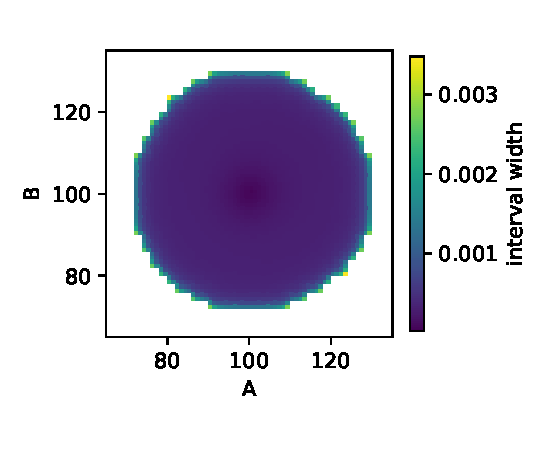
\includegraphics[width=\textwidth]{gfx/diffs.pdf}
    \end{minipage}
    \caption{Results for \autoref{model:par_bd} with truncation threshold $\epsilon=0.1$. (left) Truncations of different iterations are layered on top of each other. At higher iterations, truncations cover less area but increase in detail, due to the refinement of macro-states. The final approximation is indicated by its approximate probabilities. (right) The difference between the upper and lower bounds on the probability conditioned on the truncation.}
    \label{fig:par_bd}
\end{figure}
\begin{table}
    \centering
    \begin{tabular}{L{23mm} R{18mm} R{18mm} R{18mm} R{18mm}}
    \toprule
      & \multicolumn{4}{c}{threshold parameter $\epsilon$} \\\cmidrule(lr){2-5}
       & 1e-1 & 1e-2 & 1e-3 & 1e-4 \\
     \midrule
          total width & 1.2336 & 3.09e-02 & 5.39e-04 & 8.12e-06 \\
          max.\ width &  3.47e-03 & 9.29e-05 & 4.04e-07 & 4.65e-09 \\
          outside mass & 1.27e-02 & 1.05e-04 & 1.05e-06 & 1.06e-08 \\
         \bottomrule
    \end{tabular}
    \caption{Results for \autoref{model:par_bd} : The characteristics of the lower-upper bound intervals on the conditional probability and the mass not contained in the truncation are given.}
    \label{tab:intervals}
\end{table}
\begin{figure}
    \centering
    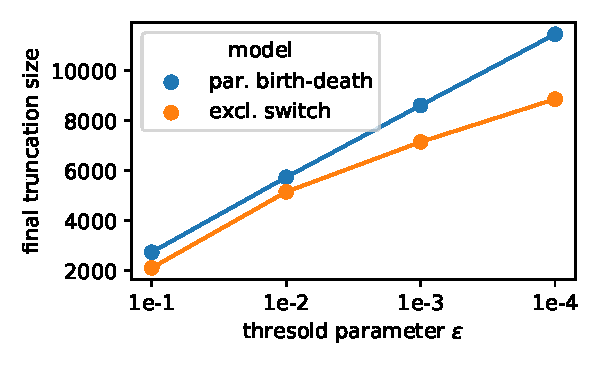
\includegraphics[scale=.8]{gfx/trunc_sizes.pdf}
	\caption[The sizes of the final truncation v.\ the threshold parameter $\epsilon$]{The sizes of the final truncation vs.\ the threshold parameter $\epsilon$ (\autoref{model:bd} and \autoref{model:excl_switch}).}
    \label{fig:excl_switch:trunc_sizes}
\end{figure}
\begin{figure}
    \centering
    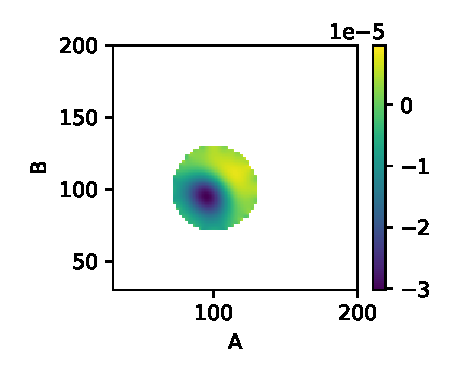
\includegraphics[width=0.48\textwidth]{gfx/par_bd_errs_0.1.pdf}
    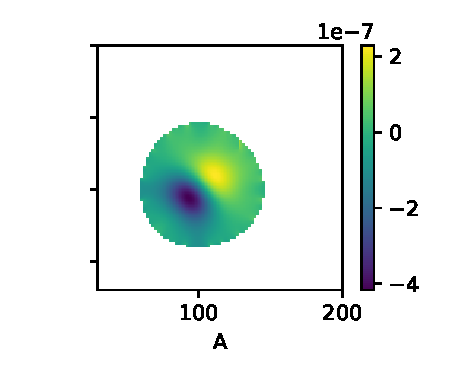
\includegraphics[width=0.48\textwidth]{gfx/par_bd_errs_0.01.pdf}
    \includegraphics[width=0.48\textwidth]{gfx/par_bd_errs_0.001.pdf}
    \includegraphics[width=0.48\textwidth]{gfx/par_bd_errs_0.0001.pdf}
    \caption{The error over the truncation wrt.\ the analytical solution}
    \label{fig:par_bd_errors}
\end{figure}

\subsection{Exclusive Switch}
The exclusive switch~\cite{barzel2008calculation}  has three different modes of operation, depending on the
DNA state, i.e.\ on whether a protein of type one or two is bound to
the DNA.

\begin{model}[Exclusive Switch]\label{model:excl_switch}
The exclusive switch model consists of a promoter region
that can express both proteins $P_1$ and $P_2$. Both can bind to the region, suppressing
the expression of the other protein. For certain parameterizations, this leads to a
bi-modal or even tri-modal behavior.
$$ D \xrightarrow{\rho_1} D + P_1 \qquad D \xrightarrow{\rho_2} D + P_2 \qquad P_1 \xrightarrow{\lambda}\varnothing \qquad P_2 \xrightarrow{\lambda} \varnothing $$
$$ D + P_1 \xrightarrow{\beta} D.P_1 \qquad D.P_1 \xrightarrow{\gamma_1} D + P_1 \qquad D.P_1 \xrightarrow{\rho_1} D.P_1 + P_1 $$
$$ D + P_2 \xrightarrow{\beta} D.P_2 \qquad D.P_2 \xrightarrow{\gamma_2} D + P_2 \qquad D.P_2 \xrightarrow{\rho_2} D.P_2 + P_2 $$
We choose parameter values $\rho_1 = 0.7$, $\rho_2 = 0.6$, $\lambda=0.02$, $\beta=0.005$, $\gamma_1 = 0.06$, and $\gamma_2 = 0.05$.
\end{model}
Since the exclusive switch models mutually exclusive binding of proteins to a single genetic locus,
we know a priori that there are exactly three distinct operating modes.
In particular are $D$, $D.P_1$, and $D.P_2$ mutually exclusive such that $X_{D}(t) + X_{D.P_1}(t) + X_{D.P_2}(t) = 1$, $\forall t\geq 0$.
This model characteristic often leads to bi-modal stationary distributions, where one or the other protein is more abundant depending on the genetic state.

Accordingly, we adjust
the initial truncation:
The state-space for the DNA states is not lumped. Instead we ``stack''
lumped approximations of the $P_1$-$P_2$ plane upon each other.
Such special treatment of DNA states is common for such models \cite{lapin2011shave}.
Using Lyapunov analysis for threshold $0.001$, we fix an initial state-space of $63\times 63$ macro-states with size $2^7$. Detailed results for different parameters $\epsilon$ are presented \autoref{tab:excl_switch}.
We compute error bounds using a worst-case analysis based on reference solutions provided by Geobound with $\epsilon_{\ell}=0.01$.
We observe a strong decrease in both upper bounds on the total absolute and maximal absolute error in the final iteration.
Interestingly, the errors between different thresholds are very close in earlier iterations.
This is mainly due to the usage of absolute errors which causes probabilities close to the mode dominate.


Using Geobound we observe that our final truncation captures the stationary mass very well (cf.\ \autoref{tab:intervals}).
We use the Geobound's lower bounds with $\epsilon_{\ell}=1e-2$ and find that the uncovered mass by the aggregation-based truncation is magnitudes lower than $\epsilon$ or close to it (for $\epsilon=0.1$).
While they capture the mass well, they are much smaller than the Geobound truncation ($\epsilon_{\ell}=0.1$) % \vw{?} 
with 16,780 states, regardless of the threshold parameter $\epsilon$.

In \autoref{fig:excl_switch:trunc_sizes}, we show the effect of the threshold parameter $\epsilon$ on the size of the final truncation.
We observe a roughly linear increase in size with an exponential decrease of $\epsilon$.
\begin{figure}
    \centering
    \includegraphics[scale=.7]{gfx/excl_switch_dist.pdf}
	\caption[Approximate stationary distribution of the exclusive switch]{The approximate stationary distribution of the exclusive switch (\autoref{model:excl_switch}) obtained with $\epsilon=\text{1e-4}$.}
    \label{fig:excl_switch:excl_switch_dist}
\end{figure}
\begin{table}
    \centering
    \begin{tabular}{L{30mm} R{15mm} R{15mm} R{15mm} R{15mm}}
    \toprule
      & \multicolumn{4}{c}{threshold parameter $\epsilon$} \\\cmidrule(lr){2-5}
       & 1e-1 & 1e-2 & 1e-3 & 1e-4 \\
     \midrule
         total width & 5.5171 & 1.5559 & 2.89e-02 & 3.71e-04 \\
         max.\ width & 1.58e-01 & 3.30e-03 & 3.47e-05 & 3.84e-07 \\
         outside mass $\leq$ & 1.52e-01 & 1.29e-03 & 2.02e-05 & 2.72e-07 \\
         \bottomrule
    \end{tabular}
	\caption[Characteristics of the lower-upper bound intervals]{Results for \autoref{model:excl_switch}: The characteristics of the lower-upper bound intervals on the conditional probability and the upper bound on mass not contained in the truncation are given.}
    \label{tab:intervals}
\end{table}

\subsection{p53 Oscillator}
We now consider a model of the interactions of the tumor suppressor p53~\cite{geva2006oscillations}. The system describes the negative feedback loop between  p53 and the oncogene Mdm2.
Species pMdm2 models a precursor to Mdm2. This model is particularly interesting due to its complex three-dimensional oscillatory behavior.
The model is ergodic with a unique stationary distribution~\cite{gupta2014scalable}.
\begin{model}[p53 Oscillator]\label{model:p53}
\begin{align*}
\varnothing \xrightarrow{k_1} \mathrm{p53} \qquad
\mathrm{p53} \xrightarrow{k_2} \varnothing \qquad
\mathrm{p53} \xrightarrow{k_4} \mathrm{p53} + \mathrm{pMdm2}
\\
\mathrm{p53} \xrightarrow{\alpha_4(\cdot)} \varnothing \qquad
\mathrm{pMdm2} \xrightarrow{k_5} \mathrm{Mdm2} \qquad
\mathrm{Mdm2} \xrightarrow{k_6} \varnothing
\end{align*}
The non-polynomial degradation reaction rate
$$
\alpha_4(x) =k_3 x_{\mathrm{Mdm2}} \frac{x_{\mathrm{p53}}}{x_{\mathrm{p53}} + k_7}\,.
$$
The parameterization based on \cite{ale2013general} is $k_1=90$, $k_2=0.002$, $k_3=1.7$, $k_4=1.1$, $k_5=0.93$, $k_6=0.96$, and $k_7 = 0.01$.
\end{model}
With the exception of propensity function $\alpha_4$, we can compute the transition rates $\bar{\alpha}_i$ using the Faulhaber formulae, as discussed in \autoref{sec:statagg:aggregation}.
We consider $\alpha_4$ separately, because it is non-polynomial and therefore, we have to make an approximation.
The fraction occurring in the non-linear propensity function $\alpha_4$ can roughly be characterized as an activation function:
Due to the low value of parameter $k_7=0.01$ we can approximate\marginpar{Note, that $\sum_{i=0}^n i / (i + k_7)$ can be solved analytically. However, the approximation presented above is much simpler to compute.}

$$\frac{x_{\mathrm{p53}}}{x_{\mathrm{p53}} + k_7}
\approx
\begin{cases}
0 & \text{if } x_{\mathrm{p53}} = 0\\
1 & \text{otherwise}
\end{cases}
$$
We use this approximation at the coarser levels of aggregation to efficiently compute the approximate transition rate $\bar{\alpha}_4$.
At the fines granularity we switch back to exact propensity function $\alpha_4$.

We now derive Lyapunov-sets for the p53 oscillator case study (Model~\ref{model:p53}). Let the Lyapunov function
\begin{equation}
    g(x) = 120 x_{\mathrm{p53}} + 0.2 x_{\mathrm{pMdm2}} + 0.1 x_{\mathrm{Mdm2}}\,.
\end{equation}
Then the drift
\begin{align}
    d(x) = & - \frac{k_3 x_{\mathrm{Mdm2}} x_{\mathrm{p53}}}{x_{\mathrm{p53}} + k_7}
            - 0.1 k_6 x_{\mathrm{Mdm2}}
            + 120 k_1 \nonumber\\
          & - 120 k_2 x_{\mathrm{p53}}
            + 0.2 k_4 x_{\mathrm{p53}}
            - 0.1 k_5 x_{\mathrm{pMdm2}} \nonumber \\
        = & - \frac{204 x_{\mathrm{Mdm2}} x_{\mathrm{p53}}}{x_{\mathrm{p53}} + 0.01}
            - 0.096 x_{\mathrm{Mdm2}}
            - 0.02 x_{\mathrm{p53}} \nonumber\\
            &- 0.0093 x_{\mathrm{pMdm2}}
            + 10800\,. \label{eq:p53_drift}
\end{align}
Clearly, $c = \sup_{x\in{S}} d(x) = 10800$.
In particular, the supremum $c$ is at the origin since all non-constant terms are negative.
The slowest rate of decrease for \eqref{eq:p53_drift} is $x_{\mathrm{p53}}$ with $x_{\mathrm{Mdm2}} = x_{\mathrm{pMdm2}} = 0$.
We are content with a superset of a Lyapunov set \eqref{eq:lyapunov_set} for some threshold $\epsilon_{\ell}$.
Therefore taking \eqref{eq:lyapunov_set}, we can solve the inequality
$$
\frac{\epsilon_{\ell}}{c}(c - 0.02 x_{\mathrm{p53}}) > \epsilon_{\ell} - 1
$$
for $x_{\mathrm{p53}}$ and 
\begin{equation}
    \frac{c}{0.02 \epsilon_{\ell}} < x_{\mathrm{p53}}\,.
\end{equation}
Therefore
\begin{equation}
\pi_{\infty}\left(\left\{x\in\mathcal{S} \mid \frac{c}{0.2\epsilon_{\ell}} < \lVert x \rVert \right\}\right) > 1 - \epsilon_{\ell}\,.
\end{equation}

Due to the exponential increase stemming from the three-dimension\-al nature of this model, we only evaluated with parameter $\epsilon=0.1$.
According to the Lyapunov analysis shown above, the area covered by an $6\times 6\times 6$ macro-states with size $2^{20}$, covers 0.9 of stationary mass.
A truncation of this same area would consist of 226,492,416 states instead of the 216 macro-states.
The model has a striking oscillatory behavior (cf.\ \autoref{fig:p53:traj}) that is reflected in its stationary distribution.
This feature is well-captured in the approximate distribution, where the oscillatory behavior leads to a complex stationary distribution (cf.\ \autoref{fig:p53:dist}).
This distribution leads to a non-trivial truncation (357,488 states) which is tailored to the main stationary mass (\autoref{fig:p53:trunc}).


\begin{figure}
    \centering
    \begin{minipage}{0.9\textwidth}
    \centering
    \includegraphics[width=\textwidth]{gfx/p53_trunc.png}
    \end{minipage}
\caption{The final truncation at original granularity derived for the p53 oscillator.}
\label{fig:p53:trunc}
\end{figure}

\begin{figure}
    \centering
    \includegraphics[width=\textwidth]{gfx/p53_traj.pdf}
    \caption{A sample trajectory illustrating the oscillatory long-run behavior. }
    \label{fig:p53:traj}
\end{figure}

\begin{figure}
    \includegraphics[width=.9\textwidth]{gfx/p53_dist.pdf}
	\caption[approximate marginal distributions of the p53 stationary distribution]{The approximate marginal distributions of the stationary distribution based on the truncation derived with $\epsilon=0.1$.}
\label{fig:p53:dist}
\end{figure}

\section{Conclusion}
State-of-the-art methods for numerically calculating the stationary distribution of Markov Population Models rely on coarse truncations of irrelevant parts of large or infinite discrete state-spaces. 
These truncations are either obtained from the stationary statistical moments of the process or from
Lyapunov theory. They are limited in shape because these methods do not take into account the detailed 
steady-state flow within the truncated state-space but only consider the average drift or stationary moments.

Here, we propose a method to find a tight truncation
that is not limited in its shape and iteratively optimizes the set based on numerically cheap solutions
of abstract intermediate models. 
It   captures the main portion of probability mass even in the case of complex behaviors efficiently.
In particular, the method represents another option, where Lyapunov analysis leads to forbiddingly large truncations.



\cleardoublepage\chapter{Analysis under Terminal Constraints}\label{ch:bridging}
% Observations of the \ac{MPM} are typically based on noisy measurements.
% In most applications, they give only partial information about the system state and are sparse in time. 
% For example, snapshots of the spread of an epidemic are typically not accurate due to false negative/positive results and limited testing. 
Many tasks, such as the analysis of rare events or the inference of agent counts under partial observations naturally introduce terminal constraints on the system.
In these cases, the system's initial state is known, as well as the system's (partial) state at a later time-point.
% Parameter inference and model analysis conditioned on such sparse and partial observations are notoriously difficult as it requires endpoint conditioned simulation of the system.
% Essentially, a model must be  analyzed  with initial conditions consistent with the observations at one time-point and under the additional constraint that its subsequent evolution is consistent with observations at later times.
The probabilities corresponding to this so-called \emph{bridging problem} are often referred to as \emph{bridging probabilities} \parencite{golightly2019efficient,golightly2011bayesian}.
For instance, if the exact, full state of the process $X_t$ has been observed at time $t=0$ and $t=T$, the bridging distribution is given by
\[
\Pr(X_t=x\mid X_{0}=x_{0},X_{T}=x_g)
\]
for all states $x$ and times $t\in [0,T]$.
Often, the condition is more complex, such that in addition to an initial distribution, a terminal distribution is present.
Such problems typically arise in a Bayesian setting, where the a priori behavior of a system is filtered such that the posterior behavior is compatible with noisy, partial observations~\parencite{broemeling2017bayesian,huang2016reconstructing}.
For example, time-series data of protein levels is available while the \acsfont{mRNA} concentration is not  \parencite{adan2017flow,huang2016reconstructing}.
In such a scenario our method can be used to identify a good truncation to analyze the probabilities of \acsfont{mRNA} levels.
% Such measurements are, for example, present in biological flow-cytometry \parencite{adan2017flow} data.
% This technique allows one to measure protein concentrations at specific time points based on fluorescent labeling.
% Such measurements are noisy due to low signal intensity and can, for instance, not measure whether a gene is active or not.
% A similar problem
% \todo{finish sentence}

% In \acp{HMM}  the backward-forward algorithm 
% decomposes the bridging problem into a forward and a backward
% analysis to calculate the marginal likelihood and calibrate the model according to noisy observations. \vw{haben wir da ein Zitat mit population structure und contin.-time? Hier das ist eigentlich eine HMM \parencite{andreychenko2012approximate} }\todo{Luca: nicely written, but what is the link with our framework?}

Bridging probabilities also appear in the context
of rare events.
Here, the rare event is the terminal constraint because we are only interested in paths containing the event.
Typically researchers have to resort to Monte-carlo simulations in combination with variance reduction techniques in such cases~\parencite{daigle2011automated,kuwahara2008efficient}.
% For instance, we may want to
% compute the probability of the rare event that the number of molecules of a certain chemical species reaches a certain cellular decision threshold \parencite{daigle2011automated,kuwahara2008efficient}.

Efficient  numerical approaches  that are not based on sampling or ad-hoc approximations have rarely been developed.

Here, we combine state-of-the-art truncation strategies based on a forward analysis~\parencite{lapin2011shave,andreychenko2011parameter} with a refinement approach that starts from an abstract \ac{MPM}
with lumped states.
We base this lumping on a grid-like partitioning of the state-space.
Throughout a lumped state, we assume a uniform distribution that gives an efficient and convenient abstraction of the original \ac{MPM}.
Note that the lumping does not follow the classical paradigm of Markov chain lumpability~\parencite{buchholz1994exact}
or its variants \parencite{dayar1997quasi}.
Instead of an approximate block structure of the transition-matrix used in that context, we base our partitioning on a segmentation of the molecule counts.
Moreover, during the iterative refinement of our
abstraction, we identify those regions of
the state-space that contribute most to the
bridging distribution.
In particular, we refine those lumped states that have a 
bridging probability above a certain threshold $\delta$ and
truncate all other macro-states. 
This way, the algorithm learns a truncation capturing most of the bridging probabilities. 
This truncation provides guaranteed lower bounds because it is at the granularity of the original model.

\section{Related Work}\label{sec:bridging:related}
\paragraph{Terminal Constraints}
The problem of endpoint constrain\-ed analysis occurs in the context of Bayesian estimation~\parencite{sarkka2013bayesian}. 
For \acp{MPM}, this problem has been addressed by \citet{huang2016reconstructing} using moment closure approximations and by \citet{wildner2019moment} further employing variational inference.
Golightly and Sherlock modified stochastic simulation algorithms to approximatively  
augment generated trajectories  \parencite{golightly2019efficient}.
% The idea is to  sample trajectories that are consistent with measurements, which requires sampling   appropriate values for latent state variables and sampling appropriate events between two observation times. 
Since a statistically exact augmentation is only possible for few simple cases, diffusion approximations \parencite{golightly2005bayesian} and moment approximations \parencite{milner2013moment} have been employed.
Such approximations, however, do not give any guarantees on the approximation error
and may suffer from numerical instabilities~\parencite{schnoerr2014validity}.

\paragraph{Rare Event Probabilities}
Another manifestation of the bridging problem is found during the estimation of first passage times and rare event analysis.
Approaches for first-passage times are often of heuristic nature ~\parencite{schnoerr2017efficient,hayden2012fluid,bortolussi2014stochastic}. Rigorous approaches yielding guaranteed bounds are currently limited by the performance of state-of-the-art optimization software~\parencite{backenkohler2019bounding}.
In biological applications, rare events of interest are typically related to the reachability of certain thresholds on molecule counts   or mode switching \parencite{strasser2012stability}.
Most methods for the estimation of rare event probabilities  rely on  importance sampling~\parencite{kuwahara2008efficient,daigle2011automated}.
For other queries, alternative variance reduction techniques such as control variates are available~\parencite{backenkohler2019control}.
Apart from sampling-based approaches, dynamic finite-state projections have been employed by \citet{mikeev2013numerical}, but are lacking automated truncation schemes.

\paragraph{State-Space Truncation}
The analysis of countably infinite state-spaces is often handled by a pre-defined truncation~\parencite{kwiatkowska2011prism}.
Sophisticated state-space truncations for the (unconditioned) forward analysis have been developed to give lower bounds and rely on a trade-off between computational load and tightness of the bound~\parencite{munsky2006finite,lapin2011shave,andreychenko2011parameter,henzinger2009sliding,mikeev2013fly}.

\paragraph{Reachability in Verification}
Reachability --~relevant in the context of probabilistic verification \parencite{bortolussi2014stochastic,neupane2019stamina}~-- is a bridging problem where the endpoint constraint is the visit of a set of goal states.
Backward probabilities are commonly used to compute reachability likelihoods \parencite{amparore2013backward,zapreev2006safe}.
Approximate techniques for reachability, based on moment closure and stochastic approximation, have also been developed in \parencite{bortolussi2014stochastic,Bortolussi18infcomp}, but lack error guarantees. 

\paragraph{Hidden Markov Models}
There is also a conceptual similarity between computing bridging probabilities and the forward-backward algorithm for computing state-wise posterior marginals in \acfp{HMM}~\parencite{rabiner1986introduction}. Like \acp{MPM}, \acp{HMM} are a generative model that can be conditioned on observations. We only consider two observations (initial and terminal state) that are not necessarily noisy but the forward and backward probabilities admit the same meaning.


\section{Backwards Probabilities}
Let $x_g\in \mathcal{S}$ be a fixed goal state.
Given the terminal constraint 
\begin{equation*}
	\Pr(X_T=x_g)=1 \text{ for some }T\geq 0\,,
\end{equation*}
we are interested in the so-called backward probabilities
\begin{equation}\label{eq:back_probs}
\beta(x_i, t) = \Pr(X_T=x_g\mid X_t = x_i),\quad t\leq T\,.
\end{equation}
Note that $\beta(\cdot, t)$ is a function of the conditional event and thus is no probability distribution over the state-space.
Instead $\beta(\cdot, t)$ gives the reaching probabilities for all states over the
time span of $[t, T]$.
To compute these probabilities, we can employ the Kolmogorov backward equation
\begin{equation}\label{eq:backward}
\frac{d}{dt}\beta(t) = Q\beta(t)\,,
\end{equation}
where we use the same vectorization to construct $\beta(t)$ as we used
for $\pi(t)$.
The above equation is integrated backwards in time and yields the reachability
probability for each state $x_i$ and time $t<T$ of ending up in $x_g$ at time $T$.
Similar to the \ac{CME} \eqref{eq:cme}, we can state a backward chemical master equation
\begin{equation}\label{eq:bcme}
    \frac{d\beta}{dt}({x}, t) =
    \sum_{j=1}^{n_R}\left(
        \beta( x,t) - \beta( x+ v_j,t)
    \right)\alpha_j({x})\,.
\end{equation}

The state-space of many \acp{MPM}, even simple ones, is countably infinite.
In this case, we have to truncate the state-space to a \emph{reasonable}
finite subset.
The choice of this truncation heavily depends on the goal of the
analysis.
If one is interested in the most ``common'' behavior, for example,
a dynamic mass-based truncation scheme is most appropriate \parencite{mikeev2019approximate}.
Such a scheme truncates states with small probability during the numerical integration.
However, common mass-based truncation schemes are not as useful for the
bridging problem. This is because trajectories that meet
the specific terminal constraints can be far off the main bulk of the
probability mass.
We solve this problem by a state-space lumping in connection with an
iterative refinement scheme.


\section{Bridging Distribution}\label{sec:bridge_dist}
The process' probability distribution given both initial and terminal constraints is formally described  by
the conditional probabilities
\begin{equation}\label{eq:bridge_dist}
    \gamma(x_i, t) = \Pr(X_t = x_i \mid X_0 = x_0, X_T = x_g)\,,
\end{equation}
for $0\leq t\leq T$.
for fixed initial state $x_0$ and terminal state $x_g$.
We call these probabilities the \emph{bridging probabilities}.
It is straight-forward to see that      $\gamma$ admits the
factorization
\begin{equation}\label{eq:bridge_fact}
    \gamma(x_i, t) = \pi(x_i, t)\beta(x_i, t)/\pi(x_g, T)
\end{equation}
due to the Markov property.
The normalization factor, given by the reachability probability 
\[
	\pi(x_g, T)=\beta(x_0, 0)\,,
\]
ensures that $\gamma(\cdot, t)$ is 
a distribution for all time points $t\in[0,T]$.
We call each $\gamma(\cdot, t)$ a   \emph{bridging distribution}.
From the Kolmogorov equations \eqref{eq:forward}\turnto{eq:forward} and \eqref{eq:backward}
we can obtain both the forward probabilities $\pi(\cdot, t)$ and the backward probabilities
$\beta(\cdot, t)$ for $t< T$.


We can easily extend this procedure to deal with hitting times
constrained by a finite time-horizon by making the goal state $x_g$ absorbing.


\begin{example}
In \autoref{fig:bd_bridge} we plot the forward, backward, and bridging probabilities for \autoref{model:bd}\turnto{model:bd}.
The probabilities are computed on a $[0,100]$ state-space truncation.
The approximate forward solution $\hat\pi$ shows how the probability mass drifts upwards towards the stationary distribution $\text{Poisson}(100)$. The backward probabilities are highest for states below the goal state $x_g=40$.
This is expected because upwards drift makes reaching $x_g$ more probable for ``lower'' states.
Finally, the approximate bridging distribution $\hat\gamma$ can be recognized to be proportional to the product of forward $\hat\pi$ and backward probabilities $\hat\beta$.
\begin{figure}[htb]
    \centering
    \includegraphics[width=\textwidth]{gfx/bridging_bd.pdf}
	\caption[Forward, backward, and bridging probabilities for \autoref{model:bd}]{Forward, backward, and bridging probabilities for \autoref{model:bd} with initial constraint $X_0=0$ and terminal constraint $X_{10}=40$ on a truncated state-space. Probabilities over $0.1$ in $\hat\pi$ and $\hat\beta$ are given full intensity for visual clarity. %$\hat\gamma$ is normalized using the reaching probability.
    The lightly shaded area ($\geq 60$) indicates a region being more relevant for the forward than for the bridging probabilities.}
    \label{fig:bd_bridge}
\end{figure}
\end{example}

\section{Bridge Truncation via Lumping Approximation}\label{sec:bridging:method}
We first discuss the truncation of countably infinite state-spaces
to analyze backward and forward probabilities (\autoref{sec:bridging:fsp}).
To identify effective truncations we employ a lumping scheme.
Finally, in \autoref{sec:bridging:alg} we present an iterative refinement algorithm
yielding a suitable truncation for the bridging problem.

\subsection{Finite State Projection}\label{sec:bridging:fsp}
Even in simple models such as a birth-death Process (\autoref{model:bd}), the
reachable state-space is countably infinite.
Direct analyzes of backward \eqref{eq:back_probs} and forward equations \eqref{eq:forw_prob}\turnto{eq:forw_prob} are often infeasible.
Instead, the integration of these differential equations requires working
with a finite subset of the infinite state-space \parencite{munsky2006finite}.
If states are truncated, their incoming transitions from states that are not truncated can be re-directed to a \emph{sink state}.
The  accumulated probability in this sink state is then used
as an error estimate for the forward integration scheme.
Consequently, many truncation schemes, such as dynamic truncations \parencite{andreychenko2011parameter}, aim to minimize the
amount of ``lost mass'' of the forward probability.
We use the same truncation method but base the truncation on bridging probabilities rather than the forward probabilities.
% We redirect incoming transitions of truncated states to the sink state.
% For all truncated states, we capture the
% corresponding incoming probability mass in a single sink state.

\subsection{Iterative Refinement Algorithm}\label{sec:bridging:alg}
The iterative refinement algorithm (\autoref{alg:refinement}) starts with a set of large macro-states
that are iteratively refined, based on approximate solutions
to the bridging problem.
We start by constructing square macro-states of size
$2^m$ in each dimension for some $m\in\mathbb{N}$ such that they form a large-scale grid $\mathcal{S}^{(0)}$.
Hence, each initial macro-state has a volume of ${\left(2^m\right)}^{n_S}$.
This choice of grid size is convenient because we can halve states
in each dimension.
Moreover, this choice ensures that all states have equal volume
and we end up with states of volume $2^0=1$ which is
equivalent to a truncation of the original non-lumped state-space.

An iteration of the state-space refinement starts by computing both the
forward and backward probabilities (\autoref{line:forw} and \autoref{line:backw})  via integration of \eqref{eq:forward}\turnto{eq:forward} and
\eqref{eq:backward}, respectively, using
 the lumped $\hat Q$-matrix.
Based on the resulting approximate forward and backward probabilities, we
  compute an approximation of the
bridging distributions (\autoref{line:bridge}).
This is done for each time-point in an equispaced grid on $[0,T]$.
The time grid granularity is a hyper-parameter of the algorithm.
If the grid is too fine, the memory overhead of storing backward $\hat\beta^{(i)}$
and forward solutions $\hat\pi^{(i)}$ increases.
{We denote the approximations with a hat (e.g.\ $\hat{\pi}$) rather than a bar (e.g.\ $\bar{\pi}$) to indicate that not only the lumping approximation but also a truncation is applied and similarly for the $Q$-matrix.}
If, on the other hand, the granularity is too low, too much of
the state-space might be truncated.
Based on a threshold parameter $\delta>0$
states are either removed or split (\autoref{line:refine}), depending on
the mass assigned to them by the approximate bridging
probabilities $\hat\gamma^{(i)}_t$.
A state can be split by the \texttt{split}-function which
halves the state in each dimension.
Otherwise, it is removed.
Thus, each macro-state is either split into $2^{n_S}$ new states or removed
entirely.
The result forms the next lumped state-space $\mathcal{S}^{(i)}$.
 The   $Q$-matrix is adjusted (\autoref{line:update_q}) such that transition rates  for $\mathcal{S}^{(i)}$  are calculated according to 
 \eqref{eq:lumped_q}. 
 Entries of truncated states are removed from the transition matrix. Transitions leading to them are
re-directed to a sink state (\autoref{sec:bridging:fsp}).
After $m$ iterations (we started with states of side lengths $2^m$)
we have a standard \ac{FSP} scheme
on the original model tailored to
computing an approximation of the bridging distribution.
\begin{algorithm}[htb]
\SetKwFunction{Split}{split}
\SetKwInOut{Input}{input}
\SetKwInOut{Output}{output}
\Input{initial partitioning $\mathcal{S}^{(0)}$, truncation threshold $\delta$}
\Output{approximate bridging distribution $\hat\gamma$}
\For{$i=1,\dots,m$}{
    ${\hat\pi}^{(i-1)}_t\leftarrow $ approximate forward equation on $\mathcal{S}^{(i)}$\label{line:forw}\;
    ${\hat\beta}^{(i-1)}_t\leftarrow $ approximate backward equation on $\mathcal{S}^{(i)}$\label{line:backw}\;
    ${\hat\gamma}^{(i)}_t\leftarrow {\hat\beta}^{(i)} {\hat\pi}^{(i)}/\hat\pi(x_g,  T)$\label{line:bridge}\tcc*{approx. bridging}
    $\mathcal{S}^{(i)}\leftarrow \emptyset$\;
    \ForEach{$\bar{x}\in\mathcal{S}^{(i)}$}{
        \If{
            $\exists t.{\hat\gamma}^{(i)}_t(\bar{x})\geq \delta$\label{line:refine}\tcc*{refinement}
        }{
            $\mathcal{S}^{(i)}\leftarrow \mathcal{S}^{(i)} \cup \Split(\bar{x})$\label{line:union}\;
        }}
        update $\hat{Q}$-matrix\label{line:update_q}\;
}
\Return ${\hat\gamma}^{(i)}$\;
    \caption{Iterative refinement for the bridging problem}
    \label{alg:refinement}
\end{algorithm}

In \autoref{fig:refinement} we give a demonstration of how
\autoref{alg:refinement} works to refine the state-space
iteratively. Starting with an initial lumped state-space $\mathcal{S}^{(0)}$ covering a large area of the state-space,
repeated evaluations of the bridging distributions are performed.
After five iterations the remaining truncation includes all states
that significantly contribute to the bridging
probabilities over the times $[0,T]$.
\begin{figure}[tb]
    \centering
    \includegraphics[width=\textwidth]{gfx/refinement.png}
	\caption[State-space refinement algorithm on two parallel unit-rate arrival processes]{The state-space refinement algorithm on two parallel unit-rate arrival processes. The bridging problem from $(0,0)$ to $(64, 64)$ and $T=10$ and truncation threshold $\delta=\e{5}{-3}$. States with a bridging probability below $\delta$ are light grey. The macro-state containing the goal state is marked in black. The initial macro-states are of size $16\times 16$.}
    \label{fig:refinement}
\end{figure}

% das ist nicht spezifisch für rare events. es kann genauso gut sein dass bei einem rare event die hauptmasse der forward in der truncation bleibt.
It is important to realize that determining the most relevant states is \emph{the} main challenge.
The above algorithm solves this problem by considering only those parts of the state-space that contribute most to the bridging probabilities.
The truncation is tailored to this condition and might ignore regions that are likely in the unconditioned case.
For instance, in \autoref{fig:bd_bridge} the bridging probabilities mostly remain below a population threshold of $\#X=60$ (as indicated by the lighter/darker coloring), while the forward probabilities mostly exceed this bound. Hence, in this example a significant portion of the forward probabilities $\hat\pi_t^{(i)}$  
 is captured by the sink state. However, the condition in \autoref{line:refine} of \autoref{alg:refinement} ensures that
states contributing significantly to $\hat\gamma_t^{(i)}$ will be kept and refined in the next iteration.
 


\section{Results}\label{sec:bridging:results}
% Three examples are chemical reaction networks whose
% stochastic evolution is described through an MJP.
% The corresponding population structure is given by the 
% copy numbers of different chemical species. 
% In this application field, an important challenge is the computation of rare event probabilities \parencite{daigle2011automated,chong2017path}. 
% Rare events of interest are typically reachability of certain thresholds on molecule counts   or mode switching \parencite{strasser2012stability}. <- ist jetzt im rel work
% 
We present four examples in this section to evaluate our proposed method. 
A prototype was implemented in Python~3.8. For numerical integration we used the Scipy implementation \parencite{2020SciPy-NMeth} of the implicit method based on backward-differentiation formulas \parencite{byrne1975polyalgorithm}.
The analysis as a Jupyter notebook is made available online~\parencite{mjp_bridging}.

\subsection{Bounding Rare Event Probabilities}
We consider a simple model of two parallel Poisson processes describing the production of two 
types of agents. 
The corresponding probability distribution
has Poisson product form at all time points $t\geq 0$ and hence we can compare the accuracy of our  numerical results with the exact analytic solution.
We use the proposed approach to compute lower bounds for rare event probabilities.
These bounds are rigorous up to the approximation error of the numerical integration scheme.
However, the forward solution could be replaced by an uniformization\turnto{item:uniformization} approach for a more rigorous error control.




\begin{model}[Parallel Poisson Processes]\label{model:par_poisson}
The model consists of two parallel independent Poisson processes with unit rates.
$$ \varnothing \xrightarrow{1} A \qquad\text{and}\qquad \varnothing \xrightarrow{1} B\,. $$
The initial condition $X_0=(0,0)$ holds with probability one. After $t$ time units each species abundance
is Poisson distributed with rate $\lambda=t$.
\end{model}
We consider the final constraint of reaching a state where both
processes exceed a threshold of $64$ at time $20$.
Without prior knowledge, a reasonable truncation would have been $160\times 160$. But our analysis shows that just \num{20}\% of the states are necessary to capture over \num{99.6}\% of the probability mass reaching the
target event (cf.\ \autoref{tab:par_poisson}).
Decreasing the threshold $\delta$ leads to a larger set of states retained after truncation as more of the bridging distribution is included (cf.\ \autoref{fig:2poisson_rare}).
We observe an increase in truncation size that is approximately
logarithmic in $\delta$, which, in this example, indicates robustness of the method with respect to the choice of $\delta$.
\begin{figure}[!t]
    \centering
    \includegraphics[width=\textwidth]{gfx/truncs.png}
	\caption[State-space truncation for varying values of the
	threshold parameter $\delta$]{State-space truncation for varying values of the
    threshold parameter $\delta$: Two parallel Poisson processes under terminal constraints $X_{20}^{(A)} \geq 64$ and $X_{20}^{(B)}\geq 64$.
    The initial macro-states are $16\times 16$ such that the final
    states are regular micro states.}
    \label{fig:2poisson_rare}
\end{figure}

%\setlength{\tabcolsep}{10pt}
\begin{table}[!t]
    \centering
	{\small
    \begin{tabular}{lrrrr}
    \toprule
	    & \multicolumn{4}{c}{threshold $\delta$}\\ \cmidrule(lr){2-5} 
	    & \e{1}{-2} & \e{1}{-3} & \e{1}{-4} & \e{1}{-5} \\
    \midrule
	    $|\mathcal{S}^{(m)}|$ & $1154$ & $2354$ & $3170$ & $3898$ \\
	    $\sum_m|\mathcal{S}^{(m)}|$\hspace{-1ex} & $2074$ & $3546$ & $4586$ & $5450$ \\
	    estimate& \e{8.88}{-30} & \e{1.85}{-29} & \e{1.86}{-29} & \e{1.86}{-29} \\
	    rel.\ error& \e{5.22}{-1} & \e{3.66}{-3} & \e{3.74}{-5} & \e{9.52}{-8} \\
    \bottomrule
    \end{tabular}}
	\caption[Rare event analysis on the \autoref{model:bd}]{Estimated reachability probabilities based on varying truncation thresholds $\delta$: The true probability is
	\e{1.8625}{-29}. We also report the size of the final truncation $|\mathcal{S}^{(m)}|$ and the accumulated size of all truncations during refinement iterations (overall states) $\sum_m|\mathcal{S}^{(m)}|$.}
    \label{tab:par_poisson}
\end{table}

\paragraph{Comparison to other methods}
The truncation approach that we apply  is similar  to the one used by \citet{mikeev2013numerical} for rare event estimation.
However,  they used a given linearly biased MPM model to obtain a truncation. A general strategy to compute an appropriate biasing was not proposed.
It is possible to adapt our truncation approach to the dynamic scheme in \citet{mikeev2013numerical} where states are removed in an on-the-fly fashion during numerical integration.
% For this dynamic adaption one can change the union over all time points 
% (\autoref{alg:refinement} \autoref{line:union}) to a union
% over time intervals. \todo{L: I do not get this really? line 7 is the split. } % MB: this point is not important

A finite state-space truncation covering the same area as the initial lumping approximation would contain $25,\!600$ states.\graffito{The goal  is not treated as a single state. Otherwise, it consisted of $24,\!130$ states.}
The standard approach would be to build up the entire state-space for such a model \parencite{kwiatkowska2011prism}.
Even using a conservative truncation threshold $\delta=\e{1}{-5}$, our method yields an accurate estimate using only about a fifth (\num{5450}) of this accumulated over all intermediate lumped approximations. 
% Moreover the analysis yields intermediate distributions which we would not obtain using PRISM.

\subsection{Mode Switching}
%Next, we turn to ``mode switching'' events.
%These occur in models exhibiting a \emph{multi-modal} behavior, which are of great relevance in
%many contexts~\parencite{siegal2011emergence}. These models exhibit a multi-modal stationary distribution.
Mode switching occurs in models exhibiting   \emph{multi-modal} behavior (see \autoref{sec:multimodality} for details) when a trajectory   traverses a potential barrier from one mode
to another.
\graffito{This often is an instance
of rare-event analysis.}
Often, mode switching is a rare event and occurs in the context of gene regulatory networks where a mode is characterized by the set of genes being currently active~\parencite{loinger2007stochastic}. 
Similar dynamics also commonly occur in queuing models where a system may for example switch its operating  behavior stochastically if
traffic increases above or decreases below certain thresholds.
Using the presented method, we can get both a   qualitative and quantitative understanding of   switching
behavior without resorting to Monte-Carlo methods such as   importance sampling.
% In the most common importance sampling scheme, for example,
% rate functions are biased using linear constants, fitted according to a cross-entropy objective~\parencite{daigle2011automated}.
% These biased paths are not necessarily representative of the bridging
% distributions.
%Thus we can gain a deeper insight into
%the actual mechanics of mode switching.
% \begin{itemize}
%     \item Mode Switching as a subclass of rare event problems
%     \item Switching dynamics are of biological interest (cell cycle control, stuff like that)
%     \item Very common ``sub-module'' of more complex models
%     \item Especially hard to tackle for standard FSP methods (multi-modal stationary distribution)
% \end{itemize}

\subsubsection*{Exclusive Switch}
The exclusive switch~\parencite{barzel2008calculation}  has three different modes of operation, depending on the
\acsfont{DNA} state, i.e.\ on whether a protein of type one or two is bound to
the \acsfont{DNA}.

\begin{model}[Exclusive Switch]\label{model:excl_switch_2} The exclusive switch model consists of a promoter region
that can express both proteins $P_1$ and $P_2$. Both can bind to the region, suppressing
the expression of the other protein. For certain parameterizations, this leads to a
bi-modal or even tri-modal behavior.
\begin{gather*}
	D + P_1 \xrightarrow{\beta} D.P_1\,,\quad
	D.P1 \xrightarrow{\gamma_1} D + P_1  \,,\\
	D + P_2 \xrightarrow{\beta} D.P_2 \,,\quad
	D.P2 \xrightarrow{\gamma_2} D + P_2 \,,\\
	D.P_1 \xrightarrow{\rho_1} D.P_1 + P_1\,, \quad
    D.P_2 \xrightarrow{\rho_2} D.P_2 + P_2\,,\\
	D \xrightarrow{\rho_1} D + P_1\,,\quad
	D \xrightarrow{\rho_2} D + P_2\,,  \quad
	P_1 \xrightarrow{\lambda}\varnothing  \,,\quad
    P_2\xrightarrow{\lambda} \varnothing
\end{gather*}
The parameter values are $\rho=\e{1}{-1}$, $\lambda=\e{1}{-3}$, $\beta=\e{1}{-2}$, and $\gamma=\e{8}{-3}$.
\end{model}
Since we know a priori of the three distinct operating modes, we adjust
the method slightly:
The state-space for the \acsfont{DNA} states is not lumped. Instead we ``stack''
lumped approximations of the $P_1$-$P_2$ phase space upon each other. Special treatment of \acsfont{DNA} states is common for such models \parencite{lapin2011shave}. 

%We assess the switching dynamics from one mode to another.
To analyze the switching, we choose the transition from\graffito{Variable order: $P_1$, $P_2$, $D$, $D.P_1$, $D.P_2$.}
\[
	x_{1} = (32, 0, 0, 0, 1) 
    \quad
    \text{to}
    \quad
 x_2 = (0, 32, 0, 1, 0) 
\]
over the time interval $t\in[0,10]$.
The initial lumping scheme covers up to \num{80} molecules of $P_1$ and $P_2$ for each mode.
Macro-states have size $8\times8$ and
the truncation threshold is $\delta=\e{1}{-4}$.

In the analysis of biological switches, not only the switching probability    
%is of interest to the researcher.
%The 
but also the switching dynamics is a central part of understanding the underlying biological mechanisms.
In \autoref{fig:switching_dynamics:modes}, we therefore plot the time-varying probabilities of the gene state conditioned on the mode.
We observe a rapid unbinding of $P_2$, followed by a slow increase of the binding probability for $P_1$.
These dynamics are already qualitatively captured by the first lumped approximation (dashed lines).
% \begin{itemize}
%     \item emphasize that we not only get rare event prob.\ estimates but insights on the dynamics leading there
%     \item explain how mode switching dynamics
%     \item Compare/contrast coarse- and fine-grained
% \end{itemize}
\begin{figure}
    \centering
    \includegraphics[scale=.6]{gfx/excl_switch_modeprobs.pdf}
	\caption[Mode probabilities of the exclusive switch bridging problem]{Mode probabilities of the exclusive switch bridging problem over time for the first lumped approximation (dashed lines) and the final approximation (solid lines) with constraints $X_0=(32, 0, 0, 1, 0)$ and $X_{10}=(0,32,0,0,1)$. \label{fig:switching_dynamics:modes}}
\end{figure}
\begin{figure}
    \centering
    \includegraphics[scale=.6]{gfx/toggle_exp_occ.pdf}
	\caption[Expected occupation time]{The expected occupation time (excluding initial and terminal states) for the switching problem of the toggle switch using Hill-type functions. The bridging problem is from initial $(0,120)$ to a first passage of $(120, 0)$ in
    $t\in [0,10]$.}
    \label{fig:switching_dynamics:occ}
\end{figure}


\subsubsection*{Toggle Switch}
Next, we apply our method to  a toggle switch model exhibiting non-polynomial rate functions.
This well-known  model considers two proteins $A$ and $B$
inhibiting the production of the respective other protein~\parencite{lipshtat2006genetic}.
\begin{model}[Toggle Switch using Hill functions]\label{model:hill_toggle}
We have population types $A$ and $B$ with the following reactions and reaction rates.
$$ \varnothing \xrightarrow{\alpha_1(\cdot)} A\,,\quad \text{where}\quad \alpha_1(x) = \frac{\rho}{1 + x_B},
\qquad A \xrightarrow\lambda \varnothing $$
$$ \varnothing \xrightarrow{\alpha_1(\cdot)} B\,,\quad \text{where}\quad \alpha_1(x) = \frac{\rho}{1 + x_A},
\qquad B \xrightarrow\lambda \varnothing $$
The parameterization is $\rho=10$, $\lambda=0.1$.
\end{model}
Due to the non-polynomial rate functions $\alpha_1$ and $\alpha_2$, 
the transition rates between macro-states
 are approximated by using the continuous integral
 \[
\bar{\alpha}_1(\bar{x})\approx\int_{a-0.5}^{b+0.5} \frac{\rho}{1 + x}\, dx = \rho \left(\log{\left(b + 1.5 \right)} - \log{\left(a + 0.5 \right)} \right)
\]
for a macro-state $\bar{x}= \{a,\dots,b\}$.%\vw{explain $k$ I guess it is the mode}%\MB{we don't have mode vars here. it's just $k$ to make the expression more clear because then its essentially 1D}

We analyze the switching scenario from $(0, 120)$ to the first visit of state $(120, 0)$ up to time $T=10$. The initial lumping scheme covers up to \num{352} molecules of $A$ and $B$ and  macro-states have size $32\times32$.
The truncation threshold is $\delta=\e{1}{-4}$.
%Transition rates are computed using the above non-polynomial integral.
The resulting truncation is shown in \autoref{fig:switching_dynamics:occ}.
It also illustrates the kind of insights that can be obtained from the bridging distributions.
For an overview of the switching dynamics, we look at the expected occupation time under the terminal constraint of having entered state $(120,0)$. Letting the corresponding hitting time be 
\[
	\tau=\inf\{t\geq 0\mid X_t=(120, 0)\}\,,
\]
the expected occupation time for some state $x$ is
\[
	E\left(\int_0^{\tau}1_{=x}(X_t)\,dt\mid \tau\leq 10\right)\,.
\]
We observe that in this example the switching  behavior seems to be asymmetrical.
The main mass seems to pass through an area where initially a small number of $A$ molecules is produced followed by a total decay of $B$ molecules.


\subsection{Recursive Bayesian Estimation}
We now turn to the method's application in recursive Bayesian estimation.
This is the problem of estimating the system's
past, present, and future behavior under given observations.
Thus, the \ac{MPM} becomes a \acf{HMM}.
The observations in such models are usually noisy, meaning that we cannot infer the system state with certainty.

This estimation problem entails more general distributional constraints on terminal $\beta(\cdot,T)$ and initial $\pi(\cdot, 0)$ distributions than the point mass distributions considered up until now.
We can easily extend the forward and backward probabilities to more general initial
distributions   and terminal distributions $\beta(T)$.
%This extension is useful for estimating scenarios subject to measurement noise.
For the forward probabilities we get
\begin{equation}
    \pi(x_i, t) = \sum_j \Pr(X_t=x_i\mid X_0=x_j) \pi(x_j,0),
\end{equation}
and similarly the backward probabilities are given by
\begin{equation}
    \beta(x_i, t) = \sum_j\Pr(X_T=x_j\mid X_t = x_i) \beta_T(x_j)\,.
\end{equation}
We apply our method to an \acf{SEIR} model.
This is widely used to describe the spreading of an epidemic such as the current 
\acsfont{COVID}-19 outbreak~\parencite{he2020seir,grossmann2020importance}.
Temporal snapshots of the epidemic spread  are mostly only available for a subset of the population and suffer from   inaccuracies of diagnostic tests.
Bayesian estimation can then be used to infer the spreading dynamics given uncertain temporal snapshots.
%Therefore due to the combination of model simulation and the uncertain measurements a  problem arises.
%We demonstrate our method on such an estimation problem.
% We assume the full model including parameterization is given.

\begin{model}[Epidemic Spread]\label{model:seir}
A population of susceptible individuals can contract a disease from infected agents. In this case, they are exposed, meaning they will become infected but cannot yet infect others. After being infected, individuals change to the removed state. The mass-action reactions are as follows.
    \[ S + I \xrightarrow{\lambda} E + I\,, \quad
E \xrightarrow{\mu} I\,, \quad
    I \xrightarrow{\rho} R\,. \]
The parameter values are $\lambda=0.5$, $\mu=3$, $\rho=3$. Due to the stoichiometric invariant $X_t^{(S)} + X_t^{(E)} + X_t^{(I)} + X_t^{(R)} = \mathrm{const.}$, we can eliminate $R$ from the system.
\end{model}

We consider the following scenario:
There are $N$ individuals.
We know that initially ($t=0$) one individual is infected and the rest is susceptible.
At time $t=0.3$ all individuals are tested for the disease.
The test, however, only identifies infected individuals with probability
$p_{\text{tp}}= 0.99$.
Moreover, the probability of a false positive is $p_{\text{fp}} = 0.05$.
\marginpar{The false positive probability is the same for all non-infected invididuals.}
The random variable $Y_t$ models the measurement likelihood at time $t$.
Based on the description above
\begin{multline*}
	\Pr(Y_t=\hat{n}_I\mid X_t^{(I)} = n_I)\\
	=
	\sum_{k=0}^{\hat{n}_I} B(k; {n_I}, p_{\text{tp}}) B(\hat{n}_I - k ; N - n_I, p_{\text{fp}})
%%%%%%%%\binom{N - n_I}{\hat{n}_I - k}\\
%%%%%%%%	p_{\text{tp}}^k (1-p_{\text{tp}})^{n_I - k} p_{\text{fp}}^{\hat{n}_I - k} (1 - p_{\text{fp}})^{N - n_I - \hat{n}_I - k}
\end{multline*}
where $B$ is the binomial probability mass function and
\[
	B(k; n, p) = \binom{n}{k}p^k(1 - p)^{n -  k}\,.
\]
We like to identify the distribution given both the initial state and the measurement at time $t=0.3$.
In particular, we want to infer the distribution over the latent counts of  $S$ and $E$ by
% The question we like to answer is whether the number of infected exceeds the threshold $k=100$ in the time interval $[t,2t]$.
  \emph{recursive Bayesian estimation}.

% The first sub-problem is the estimation of the posterior distribution at time $t$ given the measurement.
The posterior for $n_I$ infected individuals at time $t$, given measurement $Y_t=\hat{n}_I$ can be computed using  Bayes' rule
\begin{multline}\label{eq:bayes_posterior}
	\Pr(X_t^{(I)}=n_I\mid Y_t=\hat{n}_I, X_0=x_0)\\ \propto \Pr(Y_t=\hat{n}_I\mid X_t^{(I)} = n_I)\Pr(X_t^{(I)}=n_I\mid X_0=x_0)\,.
\end{multline}
This problem is an extension of the bridging problem discussed up until now.
The difference is that the terminal posterior   is   estimated it using the result of the lumped forward equation and the measurement distribution using~\eqref{eq:bayes_posterior}.
Based on this estimated terminal posterior, we compute the bridging probabilities and refine the truncation tailored to the location of the posterior distribution.
In \autoref{fig:seir:dyn}, we illustrate the bridging distribution between the terminal posterior and initial distribution.
In the context of filtering problems this is commonly referred to as smoothing.
Using the learned truncation, we can obtain the posterior distribution for the number of infected individuals at $t=0.3$ (\autoref{fig:seir:t}).
Moreover, can we infer a distribution over the unknown number of susceptible and exposed individuals (\autoref{fig:latent}).
\begin{figure}[t]
    \myfloatalign
	\subfloat[Prior and posterior dynamics]
	{\label{fig:seir:dyn}
	\includegraphics[width=0.48\linewidth]{gfx/seir_prior_posterior.pdf}}
	\subfloat[Beliefs and likelihood at $t=0.3$]
	{\label{fig:seir:t}
	\includegraphics[width=0.48\linewidth]{gfx/posterior.pdf}}
	\caption[Bayesian estimation on the \ac{SEIR} model]{
	    (a) A comparison of the prior dynamics and the posterior smoothing (bridging) dynamics.
	    (b) The prior, likelihood, and posterior of the number of infected individuals $n_I$ at time $t=0.3$ given the measurement $\hat{n}_I=30$.}
\end{figure}
\begin{figure}
	\centering
    \includegraphics[width=.6\linewidth]{gfx/prior_posterior.pdf}
	\caption[Prior and posterior (\ac{SEIR})]{\label{fig:latent}
	    The prior and posterior distribution over the latent types $E$ and $S$ at time $t=0.3$.}
\end{figure}

% Using the posterior \eqref{eq:bayes_posterior} of the first sub-problem, we can proceed and analyze the bridging problem from using the terminal constraint of the infected population exceeding threshold $k$.
% To this end this area of the state-space is made absorbing and we can proceed as before.
\section{Conclusion}
The analysis of \acp{MPM} with constraints on the initial and terminal behavior is an important part of many probabilistic inference tasks such as parameter estimation using Bayesian or maximum likelihood estimation, inference of latent system behavior, the estimation of rare event probabilities, and reachability analysis for the verification of temporal properties.  
If endpoint constraints correspond to atypical system behaviors, 
standard analysis methods fail
as they have no strategy to identify those parts of the state-space relevant for meeting the terminal constraint. 


Here, we proposed a method that is not based on stochastic sampling and statistical estimation 
but provides a direct numerical approach.
It starts with an abstract lumped model, which is iteratively refined such that only those parts of the model are considered that contribute to the  
probabilities of interest.
In the final step of the iteration, we operate at the granularity of the original model and compute lower bounds for these bridging probabilities that are rigorous up to the error of the numerical integration scheme.
%To achieve accurate bounds, appropriate error tolerances for the numerical integration have to be chosen.

Our method exploits the population structure of the model, which is present in many important application fields of \acp{MPM}.
% As with any direct method based on truncations, our approach is limited to models where population sizes remain relatively small.
Based on experience with other work based on truncation, the approach can be expected to scale up to at least a few million states~\parencite{mikeev2011efficient}.
Compared to previous work, our method neither relies on approximations of unknown accuracy nor additional information such as a suitable change of measure in the case of importance sampling.
It only requires a truncation threshold and an initial choice for the macro-state sizes.
% Alternatively, uniformization can be applied to strengthen the precision guarantees \parencite{mateescu2010fast}.\MB{for backward solutions too?; uniformization does not fit with the paragraphs opening; schon oben}

In future work, we plan to extend our method to hybrid approaches, in
which a moment representation is employed for large populations while discrete counts are maintained for small populations.
Moreover, we will apply our method to model checking  where constraints are described by some temporal logic \parencite{hajnal2019data}.

\cleardoublepage\chapter{Rare Event Probabilities}\label{ch:is}
Rare events are events that occur with very low probability.
Such events can be, for example, the die-out of some population or the switching of a multimodal system across some potential barrier.
In biological applications, rare events of interest are typically related to the reachability of certain thresholds on molecule counts  or mode switching \parencite{strasser2012stability}.
By their nature, most standard methods focus on regions with high probability.
As an example consider the standard \ac{SSA}:
Trajectories are generated according to the processes density.
Therefore unlikely events are exactly as unlikely to be sampled using the direct method.
Accordingly, lots of samples are necessary to even sample a rare event at all and many more to get an estimator with a reasonable variance.
Therefore, standard Monte Carlo estimation falls short for such use cases and typically analysis is done using variance reduction methods tailored to them.

The arguably most used method for rare event analysis is \acf{IS}.
This variance reduction method is very well-suited to the analysis of such events.
In a nutshell, this method alters the model's dynamics and keeps track of the \emph{likelihood ratio} between this altered and the original model.
This ratio provides an unbiased estimate of the event probability.
The main challenge is to find a ``good'' way to alter the model.
Ideally, such an alterated model should generate trajectories conditioned on the rare event with the same distribution found in the original model.
At the same time, a sufficiently convenient way of finding the alteration for a given model is necessary.

One popular approach is found in \acsfont{dwSSA} \parencite{kuwahara2008efficient,daigle2011automated}.
Therein each reaction rate is altered by some constant scalar factor.
These biasing values are identified by using pilot runs of the \ac{SSA} and a cross-entropy objective.

Here, we study using the approximate backward probabilities studies in the previous chapter as a proxy for the \emph{optimal} change of measure.
We use the backward probabilities' ratios of adjacent macro-states as a bias factor for the respective reaction propensities.
To deal with continuous time, we record backward probabilities at a pre-determined number of time points.
This way, the biases remain constant within the resulting time-intervals.
We illustrate the method and its characteristics on a set of case studies along with a comparison to the \acsfont{dwSSA} method.


\section{Related Work}
\paragraph{Importance Sampling}
Most methods for the estimation of rare event probabilities  rely on  importance sampling using constant reaction biases~\parencite{kuwahara2008efficient,daigle2011automated,chong2017path}.
This method has been extended to be state-dependent in \citet{roh2011state}.

\paragraph{Importance Splitting}
Importance Splitting is an alternative Monte Carlo estimation strategy.
In this setting \emph{promising} paths are split -- initiating new simulation runs.
These runs are then reweighted according to the specific splitting algorithm.
An early proposal of the splitting technique is the \ac{RESTART} algorithm \parencite{villen1994restart}.
Further popular iterations of this idea where, for example, fixed effort and fixed success splitting \parencite{garvels1998comparison}.
For more recent developments, we refer to \parencite{budde2017better,jegourel2013importance}.
A central problem in importance splitting is determining what constitutes a \emph{promising} path.
Algorithms rely on an \emph{importance function} as an oracle.
The (approximate) backward probabilities presented here could be used as such an importance function, as well.

\paragraph{Finite state projection}
Apart from sampling-based approaches, dynamic finite-state projections have been employed by \citet{mikeev2013numerical}, but are lacking automated truncation schemes.

\section{Importance Sampling}
Importance Sampling is  a popular variance reduction technique.
\marginpar{This explanation follows \cite[Chapter~9.7]{kroese2013handbook}.}
Typically it is applied for the Monte Carlo estimation of rare event probabilities.
The main idea, is to sample from a different distribution, the \ac{IS} density, and adjust samples using the ratio between this and the original density.
Let $f$ be the original density and the goal is to estimate
\[
    \E{\theta(X)} = \int \theta(x)f(x)\,dx\,.
\]
Now let $g$ be another density, dominating $\theta f$, i.e.\ \[g(x)\Rightarrow \theta(x)f(x) = 0\,.\] Then we can re-write the above as
\[
    \expSym_f({\theta(X)}) = \int \theta(x)f(x)\,dx = \int \theta(x) \frac{f(x)}{g(x)} g(x) dx = \expSym_g \theta(X) \frac{f(X)}{g(X)}\,.
\]
Therefore, we can replace the estimate using sampling from $f$ by an estimate using the density $g$ instead.
According to the right-hand side of this equation, the estimate using i.i.d.\ samples $X_i$, $1\leq i \leq N$
\begin{equation}\label{eq:imp_sampl}
    \hat{\expSym}(\theta(X)) = N^{-1} \sum_{k=1}^N \theta(X_k) \frac{f(X_k)}{g(X_k)}\,.
\end{equation}
The term factor
\[
    W(x) = \frac{f(x)}{g(x)}
\]
is called the \emph{likelihood ratio}.

Thus, the method hinges on finding a density $g^{*}$, that has a computable likelihood ratio and  minimizes the variance of the estimator \eqref{eq:imp_sampl}.
If $\theta(x)$ is an event, the perfect \ac{IS} \parencite[Chapter~9.7.1]{kroese2013handbook}
\[
    g^*(x) = \frac{\theta(x) f(x)}{\E{\theta(x)}}\,.
\]
Therefore the ideal \ac{IS} distribution is the conditional density
\[
    g^*(x) = f(x \mid \theta(X) = 1)\,.
\]

\section{Near-Optimal Biasing}
An \ac{MPM} can be modified to fullfill terminal constraints.
Previously, in \autoref{sec:bridge_dist}, we have seen how the endpoint constrained process can be described using the backward probabilities $\beta$.
The bridging distribution can be either computed using both backward and forward probabilities, but for us it is more instructive to consider, the bridging \ac{CME}.
This is the endpoint constrainted version of the \ac{CME}.
It depends on ratios of the backwards probabilities which act as factors to the propensity values.
Taking the derivative of $\gamma(x,t)=\pi(x,t)\beta(x,t)$, yields the bridging \ac{CME} (see also \citet{huang2016reconstructing})
\begin{equation}\label{eq:bridge_cme}
    \frac{d\gamma}{d t} ( x,t) =
    \sum_{j=1}^{n_R}\left(
        \tilde{\alpha}_j( x- v_j)\gamma( x- v_j,t) - \tilde{\alpha}_j( x)\gamma( x,t)
    \right)\,,
\end{equation}
where the propensities
\begin{equation}
    \tilde{\alpha}_j(x, t) = \alpha_j(x)\phi_j(x, t)\,.
\end{equation}
The time-dependent predilection factor
\begin{equation}\label{eq:dyn_predilection}
    \phi_j(x, t) = {\beta(x + v_j, t)}/{\beta(x, t)}\,.
\end{equation}
Equation~\eqref{eq:bridge_cme} reveals the optimal biasing scheme for \ac{IS}.
Since, we know that the ideal \ac{IS} distribution is the conditional distribution $\gamma$, the ratios
give a perfect biasing.
We use approximations of these ratios as a time and state dependent predilection functions $\phi_j$ during the stochastic simulation.

Naturally, computing \eqref{eq:bridge_cme} requires full knowledge of all backward probabilities $\beta(x, t)$ for all states $x$ and times $t$.
A full backward solution contains more information than the event probability, we are interested in.
In particular, the event probability is precisely $\beta(x_0, 0)$.
To make this approach feasible, we will use the aggregation-based approximation $\hat{\beta}$ of the backward probabilities $\beta$.
Thus, we will compute and store backward probabilities for the aggregated system for discrete time points up to $T$.
\[
    \bar{\phi}(i, j; t) = \hat{\beta}\left(\bar{x}_j, \Delta\floor*{\frac{t}{\Delta}}\right) / \hat{\beta}\left(\bar{x}_i, \Delta\floor*{\frac{t}{\Delta}}\right)
\]
Using these approximate backwards probabilities we can compute approximate predilections for the aggregated system.

In \autoref{fig:biases} we illustrate this scheme for a birth-death process (\autoref{model:bd}) with goal macro-state $[40,47]$ at $T=10$
and $X_0=0$.
\begin{figure}
    \centering
    \includegraphics[width=\textwidth]{gfx/biases.pdf}
    \caption[Approximate biasing]{\label{fig:biases}The approximate dynamic biasing (cut to $[e^{-2}, e^{2}]$) illustrated for a birth death process with macro-state size $8$ and target state $[40, 47]$ at $T=10$ for $10$ time points.}
\end{figure}
\autoref{fig:biases} clearly illustrates how the biases increase towards the end increasing the push towards the goal state the farther time progresses.
Since by the approximation assumption, all constituent states of a macro-state are treated as equivalent, the macro-state biases are transferred to the micro-states.
Depending on the scenario, this interpolation could be replaced by other schemes, such as nearest neighbor interpolations.
In fact, such an approach might be better suited in the example above, where we aim to push the process to a specific micro-state.

The discrete steps in the time domain are kept.
This enables the application of an adjusted \ac{SSA} that can deal with piecewise constant rate functions in the waiting time distributions.
This algorithm is discussed in the following section.

\section{Non-homogeneous Stochastic Simulation}
We are changing the rate bias dynamically over fixed intervals of the time-domain.
Therefore we cannot use the default \ac{SSA}.
With \autoref{alg:ssa_dyn} we present a version of the \acl{SSA} that simulates trajectories of a system with such dynamically changing biases.
The main change is the handling of the time-discrete changes in the loop in \autoref{line:tloop}.
Here it is tested, in which time interval the sampled jump will take place.
Therefore rates are recomputed each time the algorithm jumps forward one time-interval.

Let us first consider how exactly the jump time distribution changes.
A time-inhomogeneous exponential has the cdf
\[
    F(t) = 1 - \exp\left(-\int_0^t \lambda(s)\,ds\right)\,.
\]
Accordingly, the pdf
\[
    f(t) = \lambda(t)\exp\left(-\int_0^t \lambda(s)\,ds\right)\,.
\]
Since we compute the biases for fixed intervals, we have an exponential model with a piecewise constant rate function.
In \autoref{fig:bias_ssa:pce}, we give an example of such a distribution.
Assume, we have an increasing sequence of time points $\tau_0=0, \tau_1, \tau_2, \tau_3, \dots$ with corresponding rates $\lambda_i >0$.
The piecewise constant hazard function
\[
    \lambda(t) = \begin{cases}
        \lambda_1, & \text{if } \tau_0 \leq t \leq \tau_1\\
        \lambda_2, & \text{if } \tau_1 < t \leq \tau_2\\
        \lambda_3, & \text{if } \tau_2 < t \leq \tau_3\\
        \quad\vdots
    \end{cases}\,.
\]
We can give the pdf using a case distinction as
\begin{equation}
    f(t) = \begin{cases}
        f_1(t), & \text{if }\tau_0 \leq t \leq \tau_1\\
        f_2(t), & \text{if }\tau_1 < t \leq \tau_2\\
        f_3(t), & \text{if }\tau_2 < t \leq \tau_3\\
        \quad\vdots
    \end{cases}\,,
\end{equation}
where, letting $\Delta_k = \tau_k - \tau_{k-1}$, the piecewise densities
\[
    f_k(t) = \lambda_k \exp \left( -\sum_{i=1}^{k-1}\Delta_i\lambda_i - \lambda_k\left(t - \tau_{k-1}\right)\right)\,.
\]
Similarly, the cdf
\begin{equation}
    F(t) = 1 - \begin{cases}
        S_1(t), & \text{if }\tau_0 \leq t \leq \tau_1\\
        S_2(t), & \text{if }\tau_1 < t \leq \tau_2\\
        S_3(t), & \text{if }\tau_2 < t \leq \tau_3\\
        \quad\vdots
    \end{cases}\,,
\end{equation}
where the component survival functions
\[
    S_k(t) = \exp \left( -\sum_{i=1}^{k-1}\Delta_i\lambda_i - \lambda_k\left(t - \tau_{k-1}\right)\right)\,.
\]
The sampling from this density --~necessary in the stochastic simulation~-- uses an inverse transform.
This transform is most concisely expressed in lines \ref{line:jump_start}--\ref{line:update_t} of the pseudocode in \autoref{alg:ssa_dyn}.
The uniform random sample $X$ is checked against the probability mass of the current time interval.
The mass follows an exponential distribution with the current exit rate $a_0$.
In each iteration we recompute the rate $a_0$ and advance the time until the correct interval is identified.
Finally, in \autoref{line:update_t} the jump time is computed.
In \autoref{fig:bias_ssa:pce}, we illustrate the probability density function of an exponential distribution with a piecewise constant rate function.
Along with the pdf, an empirical distribution is presented, which samples were generated by the algorithm described here.

Since the jump time is determined after this part, the reaction selection uses the rates of this time-interval.
The probability of a reaction $j$ being selected is proportional to its biased reaction rate $\alpha_{i,j}'$ (\autoref{line:sample_dyn_r}).

The sampling of successive reactions is performed until the predefined termiantion function $\Theta$ is true.
Typically this means reaching some time-horizon $T>0$, i.e.\ $\Theta(s, t)=t>T$.
\begin{algorithm}
\SetKwInOut{Input}{input}
\SetKwInOut{Output}{output}
    \Input{$\pi_0, \theta, \Theta$}
    \Output{sample weighted by the likelihood ratio}
    %$\tau \leftarrow$ empty list\;
    $s\sim\pi_0$; $t\leftarrow 0$; $j\leftarrow 1$; $w\leftarrow 1$\;
    \Loop{\label{line:outer_loop}}{
        %$\tau\leftarrow \text{append}(\tau, (s, t))$\;
        $X\sim U[0,1]$\label{line:jump_start}\;
        $a_0\leftarrow\sum_i\alpha_{i,j}'(s)$\tcc*[r]{exit rate}
        $\delta\leftarrow t_{j+1} - t$\tcc*[r]{rest of time interval}
        $\Delta\leftarrow 0$\tcc*[r]{time offset}
        $\tau \leftarrow t$\tcc*[r]{start of the current component}
        \While{$X>1 - \exp(-a_0 \delta-\Delta)$\tcc*[r]{find interval}\label{line:tloop}}{
            $\Delta\leftarrow \Delta + a_0\delta$\;
            $\tau\leftarrow \tau + \delta$\;
            $j\leftarrow j+1$\;
            $\delta\leftarrow $ time-interval width\;
            $a_0\leftarrow\sum_i\alpha_{i,j}'(s)$\label{line:jump_end}\tcc*[r]{exit rate}
        }
        $\delta \leftarrow - ( \log(1-X) + \Delta )/{a_0}$\;

        \If{$\Theta(s, \tau + \delta)$}{
            \Return $\theta(s, \tau) w$
        }
        $k\leftarrow$ sample $i$ with probability $\alpha_{i,j}'(s)/\sum_i\alpha_{i,j}'(s)$\label{line:sample_dyn_r}\;
        ${\ell}_{1} \leftarrow \alpha_{k,j}'(s) \exp\left(-\Delta - \delta a_0\right)$\;
        ${\ell}_{0} \leftarrow \alpha_k(s) \exp\left(- (\tau + \delta - t) \sum_i\alpha_i(s)\right)$\;
        $w\leftarrow w\; {\ell}_0 / {\ell}_1$\label{line:update_w}\tcc*[r]{update likelihood ratio}
        $t \leftarrow \tau + \delta$\label{line:update_t}\tcc*[r]{update time}
        $s\leftarrow s + v_k$\tcc*[r]{update state}
    }
    \caption{\label{alg:ssa_dyn}A weighted sample of the rare event}
\end{algorithm}

In \autoref{fig:bias_ssa}, we illustrate the algorithms result using the biases discussed in the previous section.
\begin{figure}
    \centering
	\subfloat[Piecewise constant rate function]
    {\label{fig:bias_ssa:pce}\includegraphics[width=.5\textwidth]{gfx/piecewise_c_exp.pdf}}
    \subfloat[Biased SSA simulations]
    {\includegraphics[width=.5\textwidth]{gfx/biased_SSA.pdf}}
    \caption[Bias interpolation \& biased \ac{SSA}]{\label{fig:bias_ssa}}
    \caption[Importance Sampling using piecewise constant jump distributions]{Importance Sampling using piecewise constant jump distributions: (a) A piecewise constant rate function is induced by the biases changing at discrete time points. (b) We can simulate the system using piecewise constant biases.}
\end{figure}

%\begin{figure}[htb]
    %\centering
    %\includegraphics[width=\textwidth]{gfx/poisson_sims_and_biases.pdf}
    %\caption[Dynamic biasing for the Poisson process]{\label{fig:poisson_rare}The dynamic biasing of a Poisson process with rate 10 based on a lumping of \num{10} states.}
%\end{figure}

\begin{figure}[htb]
    \centering
    \includegraphics[width=\textwidth]{gfx/bd_is.pdf}
    \caption[Dynamic biasing for the Poisson process]{\label{fig:bd_rare}The dynamic biasing of a birth-death process lumping of \num{10} states and the target event $X(10)=30$.}
\end{figure}
\section{Case Studies}
We implemented the methods in Python and evaluated the method on three case studies.
The first two are rather simple, but have the advantage of a known analytical distribution.
Thus, we have a reference to compare the Monte Carlo results.
In the second part, we take a look at a more challenging model -- the toggle switch.
In this example, we face non-polynomial rate functions and a bi-modal behavior.
\subsection{Two Simple Examples}
For the Poisson process we look at the event of exceeding a threshold of \num{150} before a time-horizon of $T=10$.
The lumping scheme groups \num{10} states together and records the approximate backward probabilities for \num{10} time points.
In \autoref{fig:rare_estimates:poisson}, we summarize the estimates for different sample sizes.
In this study, we observe no finite sample bias and a quick convergence to the analytical result.

In case of the birth-death process, we focus on the event of being in state \num{30} at time $T=10$.
The lumping scheme groups \num{10} states together and records the approximate backward probabilities for \num{10} time points.
In \autoref{fig:rare_estimates:birth_death}, we summarize the estimates for different sample sizes.
In this study observe no finite sample bias and a quick convergence to the analytical result.
%Here we also observe a quick convergence to the analytical result.
\begin{figure}[htb]
    \centering
    \subfloat[Poisson process]
    {\label{fig:rare_estimates:poisson}\includegraphics[width=.5\textwidth]{gfx/poisson_estimates.pdf}}
    \subfloat[Birth-death bridge]
    {\label{fig:rare_estimates:birth_death}\includegraphics[width=.5\textwidth]{gfx/bridge_estimates.pdf}}
    \caption[Estimate distribution for different sample sizes]{\label{fig:rare_estimates}Estimate distribution for different sample sizes.}
\end{figure}
\subsection{Toggle Switch}
We return to the example of the toggle switch, known from \autoref{ch:bridging}.
It notably includes two non-polynomial propensity functions.
\begin{model}[Toggle Switch using Hill functions~\parencite{lipshtat2006genetic}]\label{model:hill_toggle_rare}
We have population types $A$ and $B$ with the following reactions and reaction rates.
$$ \varnothing \xrightarrow{\alpha_1(\cdot)} A\,,\quad \text{where}\quad \alpha_1(x) = \frac{\rho}{1 + k x_B},
\qquad A \xrightarrow\lambda \varnothing $$
$$ \varnothing \xrightarrow{\alpha_1(\cdot)} B\,,\quad \text{where}\quad \alpha_1(x) = \frac{\rho}{1 + k x_A},
\qquad B \xrightarrow\lambda \varnothing $$
The parameterization is $\rho=10$, $\lambda=0.1$, and $k=1.5$.
\end{model}
The sums of non-polynomial propensity functions have no simple analytical solution as the Faulhaber formulae.
Instead, we approximate the discrete sums via an integral:
\[
\begin{split}
    \bar{\alpha}_1(\bar{x})&\approx\int_{a-0.5}^{b+0.5} \frac{\rho}{1 + kx}\, dx\\
    &= \frac{\rho}{k} \left(\log{\left(k\left(b - \frac{1}{2}\right) + 1\right)} - \log{\left(k\left(a + \frac{1}{2}\right) + 1 \right)} \right)
\end{split}
\]
In this case study, we use both, a aggregation of $5\times 5$ and $10\times10$ states.
As an initial state we fix $(100, 0)$ and the target event is
\(\{X_t^{(B)} \geq 100 \mid t\leq 10 \}\).
In \autoref{fig:hill_rare}, we illustrate the sample trajectories and their mean under the biasing of the approximate backward probabilities.
On the left-hand side, the mean bias is given over time and per reaction.
The biasing strength increases towards the time-horizon.
\begin{figure}[htb]
    \centering
    \includegraphics[width=\textwidth]{gfx/hill_toggle_is.pdf}
    \caption[Dynamic biasing for the toggle switch]{\label{fig:hill_rare}The dynamic biasing of a toggle switch based on a lumping of $10\times 10$ states.}
\end{figure}

In \autoref{fig:hill_estimates}, we provide estimates for this case study using the aggregation-based approach presented here and the popular \acsfont{dwSSA} method as a point of comparison.
\acsfont{dwSSA} \cite{daigle2011automated} essentially derives a constant bias coefficient for each reaction.
The biases are optimizes using a cross-entropy objective.
This optimization, however, needs a large number of runs in each iteration.
We used ensemble sizes of \num{1000} and \num{10000} for each iteration.
This imposes a large additional cost, since in almost all instances more than \num{10} optimization iterations were necessary, until a fraction of $0.1$ ensemble trajectories reached the rare event region.
In some instances no change of measure was found using the cross-entropy optimization.
\begin{figure}[htb]
    \centering
    \begin{minipage}{0.77\textwidth}
        \includegraphics[scale=.55]{gfx/hill_estimates.pdf}
    \end{minipage}
    \hspace{1ex}
    \begin{minipage}{0.07\textwidth}
        \includegraphics[scale=.55]{gfx/hill_estimates_legend.pdf}
    \end{minipage}
    \caption[Rare event estimates (toggle switch)]{\label{fig:hill_estimates}Rare event estimates (toggle switch with Hill functions) using different methods and sample sizes. For each scenario \num{10} estimations were performed. To the left are the \acsfont{dwSSA} results for comparison. We provide results for estimates using \num{1000} and \num{10000} estimates in each iteration of the prior parameter optimization rounds. On the right, the results for the aggregation method presented in this chapter are given for grids with $5\times 5$ and $10\times 10$ macro states.}
\end{figure}

%\begin{itemize}
    %\item more likely paths are sampled less often
    %\item sample weight distribution not normal
    %\item a high-weight tail
    %\item still unbiased, but too large ``outliers'' need to correct for many estimates that are too low. therefore many samples are necessary
    %\item less variance in agg. because paths are steared more (not better estimates though...)
%\end{itemize}
With both methods, we observe that with smaller sample sizes, the estimate tends to be smaller as well, regardless of the method.
This is due to the (non-zero) weights not being normally distributed.
There tend to be more samples with lower weight, which are compensated by few samples with a marger larger weight.
In other words, there seems to be a long tail towards to higher weights in most cases.
The theoretical estimate is still unbiased.
But the estimates which are much larger (``correcting'' the low estimates) are very infrequent.
This issue is present regardless of the chosen method.
The most clear difference is that the estimates using aggregation are spread less.
This effect is likely due to the aggregation-based biasing steering the process with more detail.
Therefore trajectories tend to be more similar --- an effect that is also appearant in the samples of \autoref{fig:hill_paths_comp}.

As a reference and baseline we consider the dynamic truncation result obtained by the \acsfont{STAR} tool \parencite{lapin2011shave}.\marginpar{\url{mosi.uni-saarland.de/tools/shave/}}
We ran the analysis using a relative tolerance of \num{1e-15} and an absolute tolerance of \num{1e-90}.
This yielded \(\Pr(X_{10}^{(B)} \geq 100) \approx \num{4.64e-60}\).
Note, that this is a lower bound to the probability since we only consider the probability at $t=10$, whereas the stopping time above considers all $t\leq 10$.
Considering this baseline, it is clear, that both methods have only slowly approach the probability's true magnitude with increasing sample size.

%\begin{itemize}
    %%\item different areas sampled
    %\item right: low weights if B increases early or A does not decrease in the end (tendency)
    %\item right: large variance in sample weights (orders of magnitude)
    %\item left: weights are closer together
    %\item conclusion: sampling true transition paths may require more than constant biasing
%\end{itemize}
In \autoref{fig:hill_paths_comp}, we compare sample paths using the technique presented here with a constant biasing scheme. 
The constant biases are obtained using a cross-entropy optimization using $10^4$ \ac{SSA} simulations in each iteration until $0.1$ of the trajectories reach the rare event region.
It is immediately clear, that the sampled trajectories differ in the paths that are sampled.
%The theoretical optimal sampling would generate trajectories proportional to the original system dynamics conditioned on reaching reaching the rare event.
We further observe a far larger range of likelihood ratios in the constant biasing case.
\begin{figure}[htb]
    \centering
    \includegraphics[scale=.6]{gfx/hill_paths_comp.pdf}
    \caption[Comparison of biased sample paths]{\label{fig:hill_paths_comp}Biased sample paths of the toggle switch using (left) the aggregation based sampling and (right) a constant biasing, determined by cross-entropy optimization \parencite{daigle2011automated}. The constant bias vector is $\approx (0.873, 26.248, 2.751, 0.00159)^{\top}$. The path color represents the relative $\log$-weights of each trajectory (darker -- higher weight).}
\end{figure}

This case study showcases the major difficulty in finding an efficient change of measure that one can encounter.
Ideally, sampled trajectories should follow the original process, conditioned on the rare event.
As in this example, constant biases might not be enough to reliably alter the dynamics in this way.
However, the approximate biasing scheme presented in this chapter, while being based on an approximation of the ideal biasing, seems to over-constrain the process and thus not explore the trajectory space sufficiently.
Consequently, both methods tend to under-estimate in a majority of cases.

\section{Conclusion}
In this chapter, we presented a novel change of measure using approximate backward probabilities.
This approach avoids the necessity of a significant number of pilot runs.
In the last example, the number of these pilot runs often exceeded the number of runs used for the estimate.
Therefore, the approach presented is a feasible alternative for cases in which the state-space size allows for an approximate solution.

We further showcased a challenge that is often emphasized too little.
This is the issue of changes of measures, that steer the process to the target region along trajectories that are significantly less likely in the original system than the conditioned paths would be.
This leads to a case where the estimate distribution is very different from a normal distribution.
Consequently, the estimates are too low in most cases, and a lot too large in very few cases.

This issue might be tackled by, using state space refinement, similar to the previous chapter.\turnto{ch:bridging}
Also, combining  backward probability approximations of differing granularity might be a viable strategy.
%\paragraph{Issues}
%\begin{itemize}
    %\item emphasize large cost of pilot runs
    %\item due to the approximative nature, the speed is often too high or too low
    %\item simultions reach the target to early: many samples with very low weight, few with high weight
    %\item the estimates are still unbiased but not approximately normally distributed, even for larger biases (make an example, that this is also the case for constant biasing)
    %\item bias strength can be adjusted such that only a portion reaches
    %\item this improves the somewhat, but may alter the biases too much and the weight distribution (sampled) is still bad
%\end{itemize}
%\paragraph{Future Work}
%\begin{itemize}
    %\item \emph{Multiple importance sampling} for different accelerations to avoid problems of under- and overacceleration
%\end{itemize}

%\ctparttext{
	%Existing Foster-Lyapunov functions often give sets that are far
	%larger necessary for a given probability bound.
	%Here, we explore the possibility to improve upon such a function
	%by \emph{local} alterations.
	%This leaves the global properties --~and thereby its guarantees~--
	%intact, while we obtain much tighter sets for
	%the same probability bounds.
%}
%\part{Foster-Lyapunov Functions}
%\cleardoublepage\section{Augmented Foster-Lyapunov Bounds}\label{ch:lyapunov}
The use of Foster-Lyapunov approaches, is often two-fold: They are used to prove ergodicity and to provide sets with a lower bound $1-\epsilon$ on their stationary probability mass.
Often practical methods focus on proving \emph{global} properties of their associated drift \parencite{gupta2014scalable,spieler2014numerical}.
In many models, simple affine functions \parencite{gupta2017finite} and even the identity \parencite{spieler2014numerical} is sufficient.
While such simple forms provide some of the necessary ease of a global analysis, the task of optimizing them with performance in mind, is much more difficult \parencite{milias2014optimization}.\marginpar{\emph{Performance} in this context means least states to cover most stationary probability mass.}

Ideally, one would have the best of both worlds: The ease of working with simple forms for the global guarantees of the Foster-Lyapunov criteria and the freedom of choice to fit efficient functions and get sets that are as small as possible.
The approach presented here achieves this by \emph{locally} altering a proposal Foster-Lyapunov function.
The presence of such a valid proposal function is necessarcy for this method.
Such a function can be identified by convex analysis, for example \parencite{gupta2014scalable} or using the approach described by \textcite{spieler2014numerical}.
Using a set of probability $>1-\epsilon$ is identified using such a functional.
On this set, the original function is then replaced by any other lower bounded function.
At the set boundary this supplementary function is \emph{phased out} and we switch back to the original function using some smooth step function.
The choice of such a supplementary function offers much room for experimentation since all the necessary global criteria.
For this function we can, for example, use any polynomial or even more variable models such as neural networks.

The procedure to identify an efficient function is thereby reduced to a simple machine learning problem.
The objective exponentially rewards negative drift yielding tight sets.
Its computation needs, in principle, all points in a sufficiently large set.
For optimization however, we switch to an approach of sampling uniformly from the augmentation set.

This method yields sets that are smaller on the order of $10^3$ for a fixed probability bound over a simple linear functional.
We study neural networks and polynomial templates as candidates for local augmentation.

\subsection{The Drift and its Properties}
The drift \eqref{eq:drift} plays a central role in this chapter.\marginpar{We explain the interpretation and give some basic use of the drift in \autoref{sec:statagg:lyapunov} on page~\pageref{sec:statagg:lyapunov}.}
\begin{equation}
	d(x; g) = Qg(x) = \sum_{j=1}^{n_R} \alpha_j(x) (g(x+v_j) -  g(x))
\end{equation}
An interesting fact about the drift is, that it is invariant to linear transforms to $g$.
That is, for a constant $b\in\mathbb{R}$, we can define $h(x)=g(x)+b$ and \( Qh(x) =Qg(x)\).
Clearly, a positive linear factor $m$ to $g$ factors out, i.e.\ $Q(f\circ g)(x)=mQg(x)$ for $f(x) = mx$, $m>0$.
Consequently, if the drift is scaled by its maximum value, the scaled version is invariant to linear
transforms of $g$:
\begin{equation}
	\frac{Q(f\circ g)(x)}{\max_{x\in\mathcal{S}}Q(f \circ g)(x)}
	=
	\frac{Qg(x)}{\max_{x\in\mathcal{S}}Qg(x)}
\end{equation}
Since the probability bounded sets $C_{\epsilon_{\ell}}$ depend on the scaled drift.
Therefore invariance under linear transformation implies that we cannot change --~especially improve~-- the tightness of the sets by such a transform.

\subsection{Local Substitution}
We use a proved Foster-Lyapunov function as a starting point.
For many relevant reaction networks, simple choices such as L1 or L2 norms are sufficient choices \parencite{spieler2014numerical}.
The resulting sets, however, are typically very large.
Tasks such as computing approximate stationary distributions on truncations set up according to these sets can be very costly.
This cost is exacerbated when a system has to be solved for a lot of different reentry matrices, which is necessary when state-wise bounds on the probability conditioned on a truncation are desired~\parencite{dayar2011bounding}.

We propose to augment the proposal function by a function, that is limited to local influence guided by the initial set.
This supplementary function is phased out asymptotically using a simple sigmoid threshold function
\begin{equation}\label{eq:threshold}
  \gamma_{k,z}(x) = \frac{1}{1+k\exp(-x - z)}\,.
\end{equation}
Thus, in a one-dimensional model the augmented Lyapunov $g'$ function becomes
\begin{equation}\label{eq:thres_lyapunov}
    g'(x) = \gamma_{k,z}(x) g(x) + (1 - \gamma_{k,z}(x)) g^*(x)\,.
\end{equation}
The threshold function $\gamma$ guarantees that $g^*$ vanishes asymptotically.
The drifts $d'$ and $d^*$ are defined accordingly.

\subsection{Illustrating Example}
Consider the example of Model~\ref{model:bd}.
The question is: What makes the perfect Foster-Lyapunov function?
Here, we are interested in the smalled set of states containing the largest amount of stationary probability mass.
\marginpar{The beauty standard may vary for other applications.}
Since we know the stationary distribution to be Poissonian, its standard confidence intervals can be used as a reference.
The confidence interval for level $1-\alpha$ of a Poisson with rate $\mu$ is
\[
\frac{1}{2}P^{-1}(\alpha/2; 2k)\le\mu\leq\frac{1}{2}P^{-1}(1-\alpha/2;{2k+2})\,.
\]
where $P^{-1}(\,\cdot\,; l)$ is the inverse \ac{CDF} of a $\chi^2_{l}$ distribution.
Thus, its the inverse of the regularized gamma function
\[
	\frac{1}{\Gamma(k/2)}\int_0^{x/2} t^{k/2 - 1} e^{-t}\,dt
\]
w.r.t.\ $x$.
This gives us the ``ideal'' intervals $[l_{\epsilon},h_{\epsilon}]$, $(l_{\epsilon},h_{\epsilon})\in\mathbb{N}^2$ such that $\pi_{\infty}([l_{\epsilon},h_{\epsilon}])=1-\epsilon$.
These sets are given as the dark area in \autoref{fig:lya_sets}.
Therefore, the perfect Lyapunov function would coincide with those sets. That is,
a function $g$ such that
\[
%	\left\{x\in\mathcal{S}\mid \frac{\epsilon}{c}Qg(x)> \epsilon - 1\right\}
	C_{\epsilon}
	=
	\left[l_{\epsilon}, h_{\epsilon}\right], \quad \forall\epsilon> 0\,.
\]

Using a simple L2 norm as an initially, i.e.\ $g(x) = x^2$, we obtain a fairly large set.
In Figure~\ref{fig:bd:truncation}, we contrast this result to the solution given by the choice of $g^*(x)=(x - 250)^2$, which gives a much tighter subset with the same guarantees.
In this case, the guarantee is that the sets contain at least 0.9 stationary probability mass.
We further demonstrate how the incorporation $g^*$ into $g$ significantly tightens the set proposed initially.
\begin{figure}[htb]
    \centering
    \includegraphics[width=.6\textwidth]{gfx/lyapunov_bd.pdf}
    \caption[Augmented Foster-Lyapunov function]{\label{fig:bd:truncation}Different example Lyapunov functions for Model~\ref{model:bd}. The drifts $d$, $d^*$, and $d'$ are scaled and the appropriate threshold for $\epsilon=0.1$ is given.}
\end{figure}


The benefit of the threshold-based construction \eqref{eq:thres_lyapunov} is that we only require $g^*$ to be non-negative.
All other properties are inherited from the proposal function.
This freedom enables the use of flexible machine learning models to search an efficient $g^*$.


\paragraph{Neural Augmentation}
The characteristics of the augmentation function $g^*$ are typically not known beforehand.
The formulation of augmented Foster-Lyapunov functions only places basic constraints on the function used:
The function needs to be non-negative and an upper bound of the drift has to be known.
Neural networks lend themselves naturally as an extremely flexible functional family.

The central piece of fitting $g^*$ is an objective function.
Since the actual sets, bounded in probability, are defined in terms of their drift, this objective needs to be a function of this drift.
A desirable augmented drift has tight level sets with more emphasis placed on its peak regions.
A natural way to express this prioritization is the objective
\[\sum_{x\in\mathcal{S}}\int_{-\infty}^{d^*(x)}\exp(y)\,dy = \sum_{x\in\mathcal{S}} \exp(d'(x)) \]
based on the scaled augmented drift.

In \autoref{fig:lya_sets} we give an example of different subsets $\left|\mathcal{C}_{\epsilon}\right|$ across different thresholds $\epsilon$.
For the augmentation we use a minimal neural network consisting of four radial basis functions and a threshold function with $z=1500$ and $k=0.01$.
While such a simple model performs well in this example, larger and higher-dimensional augmentation areas may require a more complex model.
Considering the results, we observe a marked improvement over the proposal functions performance.
\begin{figure}[htb]
\centering
\includegraphics[width=\textwidth]{gfx/lya_sets.pdf}
	\caption[Augmented v.\ proposal Lyapunov sets]{\label{fig:lya_sets}Lyapunov sets for the birth-death process for different probability thresholds $\epsilon$ for the augmented function (orange) and the proposal (green). The ``perfect'' sets are computed using the confidence interval (red).}
\end{figure}

In \autoref{fig:improvement_lyaaug}, we compare the sets of Lyapunov subsets for varying thresholds $\epsilon$ for the proposal and the augmented function.
We observe a consistent improvement that is the strongest for smaller $\epsilon$.
The overall improvement is significantly better using the linear proposal function.
This is mainly due to the better performance of the quadratic proposal compared to the linear.
The subset sizes using the augmented function is qualitatively similar for both choices of proposal function.
\begin{figure}[htb]
	\centering
	\subfloat[Linear proposal]
	{\includegraphics[width=0.48\textwidth]{gfx/lnn_improvement_linear.pdf}}
	\subfloat[Quadratic proposal]
	{\includegraphics[width=0.48\textwidth]{gfx/lnn_improvement_quadratic.pdf}}
    \caption[Subset sizes using Lyapunov-Augmentation]{\label{fig:improvement_lyaaug}The sizes of the reference Lyapunov sets compared to the sizes of the augmented Lyapunov sets along with the improvement given by the augmentation. Results are shown for both, a linear and a quadratic proposal function.}
\end{figure}

\subsection{Concluding Remarks}
The local augmentation of simpler proposal Lyapunov functions is promising.
To achieve more scalability and flexibility the method has some points that need refinement.
The most obvious aspect is the optimization of the local augmentation.
The evaluation of the objective necessitates the computation of the maximum drift.
In previous works this has also been directly used as an objective \parencite{milias2014optimization}.
This entails the evluation of the drift across the entire augmentation region (and some global reasoning).
Here, this issue has largely been ignored, but especially in higher dimensional models this may cause issues.
There it might be better, to estimate the maximal drift using a --~possibly random~-- grid of states instead of a dense state-space region.

Furthermore the design-space of augmentations is huge.
More conventional models may prove to be easier to handle, especially with respect to the objective computation.
Symbolic regression \parencite{pysr}, for example, may be a useful alternative to derive more explainable Lyapunov functions.

%\begin{model}[Competitive Spread]\label{model:comp_spread}
	%Two uncoupled parallel birth-death processes (cf.~\autoref{model:par_bd})\turnto{model:par_bd} supplemented with two Gray-Scott type reactions.
%%	https://groups.csail.mit.edu/mac/projects/amorphous/GrayScott/
%\begin{gather*}
    %\varnothing\xrightarrow{\rho} A\,, \quad
    %A\xrightarrow{\delta} \varnothing\,, \quad
    %\varnothing\xrightarrow{\rho} B\,, \quad
    %B\xrightarrow{\delta} \varnothing\,,\\
	%2A+B\xrightarrow{\nu_1}3A\,,\quad
	%2A+A\xrightarrow{\nu_2}3B\,.
%\end{gather*}
	%As a parameterization we choose $\rho = 5$, $\delta=0.1$, $\nu_1=\e{6}{-5}$, and $\nu_2=\e{6.2}{-5}$.
%\end{model}


\part{Concluding Remarks}
\cleardoublepage\chapter{Conclusion}

% ********************************************************************
% Backmatter
%*******************************************************
\appendix
%\renewcommand{\thechapter}{\alph{chapter}}
\part{Appendix}
\chapter{Additional Results \& Data}
\begin{table}[h]
    \centering
\begin{adjustbox}{angle=90}
    \begin{tabular}{L{8mm} l rrrrrrrr}
        \toprule
        \multicolumn{2}{c}{} & \multicolumn{8}{c}{iteration $i$} \\\cmidrule(lr){3-10}
         $\epsilon$ & & 1 & 2 & 3 & 4 & 5 & 6 & 7 & 8  \\
         \midrule
         \multirow{3}*{1e-1} 
         & $|\mathcal{S}^{(i)}|$ & 4,900 & 28 & 52 & 112 & 232 & 472 & 960 & 1,932 \\
         & tot.\ error & 1.91 & 1.84 & 1.73 & 1.55 & 1.29 & 9.35e-1 & 4.88e-1 & 3.54e-2\\
         & max.\ error & 3.15e-3 & 3.13e-3 & 3.08e-3 & 2.98e-3 & 2.77e-3 & 2.38e-3 & 1.57e-3 & 6.04e-5 \\
         \midrule
         \multirow{3}*{1e-2}
         & $|\mathcal{S}^{(i)}|$ & 4,900 & 52 & 104 & 208 & 464 & 988 & 2,008 & 4,052 \\
         & tot.\ error & 1.91 & 1.84 & 1.73 & 1.56 & 1.30 & 9.46e-1 & 5.01e-1 & 6.22e-4\\
         & max.\ error & 3.15e-3 & 3.13e-3 & 3.08e-3 & 2.98e-3 & 2.78e-3 & 2.39e-3 & 1.59e-3 & 8.33e-7\\
         \midrule
         \multirow{3}*{1e-3}
         & $|\mathcal{S}^{(i)}|$ & 4,900 & 84 & 152 & 300 & 652 & 1,440 & 2,996 & 6,068 \\
         & tot.\ error & 1.91 & 1.83 & 1.73 & 1.56 & 1.30 & 9.46e-1 & 5.01e-1 & 9.83e-6\\
         & max.\ error & 3.15e-3 & 3.13e-3 & 3.08e-3 & 2.98e-3 & 2.78e-3 & 2.39e-3 & 1.59e-3 & 1.14e-8\\
         \midrule
         \multirow{3}*{1e-4}
         & $|\mathcal{S}^{(i)}|$ & 4,900 & 116 & 212 & 400 & 848 & 1,872 & 3,960 & 8,060 \\
         & tot.\ error & 1.91 & 1.83 & 1.73 & 1.56 & 1.30 & 9.46e-1 & 5.01e-1 & 9.83e-6\\
         & max.\ error & 3.15e-3 & 3.13e-3 & 3.08e-3 & 2.98e-3 & 2.78e-3 & 2.39e-3 & 1.59e-3 & 1.83e-10\\
         \bottomrule
    \end{tabular}
\end{adjustbox}
    \caption{Detailed results for Model~\ref{model:par_bd}. The errors are computed wrt.\ the reference Poissonian product. The total absolute error and the maximum absolute errors are given.}
    \label{tab:par_bd}
\end{table}
\begin{table}
    \centering
	\begin{adjustbox}{caption={asd sd sad},angle=90}
    \begin{tabular}{L{8mm} l rrrrrrrr}
        \toprule
        \multicolumn{2}{c}{} & \multicolumn{8}{c}{iteration $i$} \\\cmidrule(lr){3-10}
         $\epsilon$ & & 1 & 2 & 3 & 4 & 5 & 6 & 7 & 8  \\
         \midrule
         \multirow{3}*{1e-1} 
            & $|\mathcal{S}^{(i)}|$ & 11907 & 20 & 32 & 60 & 140 & 340 & 840 & 2116 \\
            & tot.\ error $\leq$ & 1.86e0 & 1.85e0 & 1.45e0 & 1.18e0 & 9.31e-1 & 6.41e-1 & 4.67e-1 & 4.89e-1 \\
            & max.\ error $\leq$ & 1.63e-3 & 1.63e-3 & 1.55e-3 & 1.40e-3 & 1.22e-3 & 9.36e-4 & 8.40e-4 & 1.40e-3 \\
         \midrule
         \multirow{3}*{1e-2}
& $|\mathcal{S}^{(i)}|$ & 11907 & 48 & 112 & 148 & 300 & 720 & 1892 & 5156 \\
& tot.\ error $\leq$ & 1.86e0 & 1.84e0 & 1.44e0 & 1.21e0 & 9.56e-1 & 6.65e-1 & 3.41e-1 & 3.31e-2 \\
& max.\ error $\leq$ & 1.63e-3 & 1.62e-3 & 1.53e-3 & 1.39e-3 & 1.20e-3 & 9.59e-4 & 5.86e-4 & 5.37e-5 \\
         \midrule
         \multirow{3}*{1e-3}
& $|\mathcal{S}^{(i)}|$ & 11907 & 84 & 192 & 244 & 488 & 1084 & 2692 & 7152 \\
& tot.\ error $\leq$ & 1.86e0 & 1.83e0 & 1.46e0 & 1.22e0 & 9.63e-1 & 6.67e-1 & 3.37e-1 & 8.01e-4 \\
& max.\ error $\leq$ & 1.63e-3 & 2.95e-2 & 1.54e-3 & 1.39e-3 & 1.20e-3 & 9.51e-4 & 5.79e-4 & 1.09e-6 \\
         \midrule
         \multirow{3}*{1e-4}
& $|\mathcal{S}^{(i)}|$ & 11907 & 124 & 324 & 352 & 672 & 1436 & 3408 & 8864 \\
& tot.\ error $\leq$ & 1.86e0 & 1.83e0 & 1.46e0 & 1.22e0 & 9.63e-1 & 6.67e-1 & 3.37e-1 & 1.12e-5 \\
& max.\ error $\leq$ & 1.63e-3 & 3.19e-2 & 1.54e-3 & 1.39e-3 & 1.20e-3 & 9.51e-4 & 5.79e-4 & 1.28e-8 \\
         \bottomrule
    \end{tabular}
\end{adjustbox}
    \caption{Detailed results for Model~\ref{model:excl_switch}. Upper bounds on the total absolute error and the maximum absolute error are given. The worst-case errors are computed wrt.\ the reference Geobound solution with $\epsilon_{\ell}=1e-2$.}
    \label{tab:excl_switch}
\end{table}
\begin{table}[]
    \centering
\begin{tabular}{l@{\hskip 12pt}l@{\hskip 12pt}l@{\hskip 12pt}r@{\hskip 12pt}r@{\hskip 12pt}r@{\hskip 12pt}r}
\toprule
  Case study &   $n_{\lambda}$ & $\phi$ & $1-\frac{\sigma_1^2}{\sigma_0^2}$ &  slowdown &  efficiency& $\lvert P\rvert$ \\\midrule
Dimerization & 10 &$\phi_{sq}$ &  0.881641 &  1.530137 &    5.558692 &   1.621917 \\
            &    &$\phi_{c}$ &  0.965224 &  1.945588 &   14.859417 &   3.338501 \\
            &    &$\phi_{q}$ &  0.916445 &  1.625232 &    7.409904 &   1.997045 \\
            &    & $\phi_{\ell}$ &  0.868288 &  1.380344 &    5.529745 &   1.081152 \\\cmidrule{2-7}
            & 20 &$\phi_{sq}$ &  0.941153 &  1.637272 &   10.437978 &   1.842971 \\
            &    &$\phi_{c}$ &  0.964204 &  1.907999 &   14.747328 &   2.915082 \\
            &    &$\phi_{q}$ &  0.947984 &  1.747519 &   11.072422 &   2.227250 \\
            &    & $\phi_{\ell}$ &  0.931030 &  1.433401 &   10.169570 &   1.088572 \\\cmidrule{2-7}
            & 30 &$\phi_{sq}$ &  0.959517 &  1.723449 &   14.404936 &   1.972426 \\
            &    &$\phi_{c}$ &  0.962514 &  1.770936 &   15.142156 &   2.216103 \\
            &    &$\phi_{q}$ &  0.966216 &  1.847441 &   16.117387 &   2.446661 \\
            &    & $\phi_{\ell}$ &  0.945724 &  1.456432 &   12.710196 &   1.084188 \\\midrule
Dist.\ mod. & 10 &$\phi_{sq}$ &  0.619560 &  1.488483 &    1.770218 &   3.232575 \\
            &    &$\phi_{c}$ &  0.700255 &  2.241695 &    1.492171 &   8.008607 \\
            &    &$\phi_{q}$ &  0.643550 &  1.613001 &    1.743500 &   3.817641 \\
            &    & $\phi_{\ell}$ &  0.596650 &  1.459405 &    1.703170 &   2.657000 \\\cmidrule{2-7}
            & 20 &$\phi_{sq}$ &  0.697414 &  1.519425 &    2.181687 &   2.631677 \\
            &    &$\phi_{c}$ &  0.713445 &  2.706546 &    1.292838 &  10.295856 \\
            &    &$\phi_{q}$ &  0.697654 &  1.585313 &    2.092817 &   3.398235 \\
            &    & $\phi_{\ell}$ &  0.695846 &  1.473976 &    2.235418 &   2.226530 \\\cmidrule{2-7}
            & 30 &$\phi_{sq}$ &  0.712941 &  1.543068 &    2.263644 &   2.378037 \\
            &    &$\phi_{c}$ &  0.721354 &  2.874249 &    1.252541 &  10.910880 \\
            &    &$\phi_{q}$ &  0.711877 &  1.607712 &    2.164485 &   2.979704 \\
            &    & $\phi_{\ell}$ &  0.669963 &  1.522184 &    1.996300 &   2.085473 \\\midrule
Excl. switch & 10 &$\phi_{sq}$ &  0.807184 &  1.227471 &    4.239255 &   2.536479 \\
            &    &$\phi_{c}$ &  0.880285 &  1.633530 &    5.135205 &   7.411732 \\
            &    &$\phi_{q}$ &  0.849082 &  1.312416 &    5.067770 &   3.639250 \\
            &    & $\phi_{\ell}$ &  0.783459 &  1.195821 &    3.874778 &   2.090101 \\\cmidrule{2-7}
            & 20 &$\phi_{sq}$ &  0.856593 &  1.263340 &    5.539683 &   2.206154 \\
            &    &$\phi_{c}$ &  0.910480 &  1.864405 &    6.011256 &   9.441336 \\
            &    &$\phi_{q}$ &  0.867987 &  1.317958 &    5.765884 &   3.140806 \\
            &    & $\phi_{\ell}$ &  0.825518 &  1.243075 &    4.627662 &   1.981143 \\\cmidrule{2-7}
            & 30 &$\phi_{sq}$ &  0.869165 &  1.298893 &    5.905196 &   2.059415 \\
            &    &$\phi_{c}$ &  0.921019 &  1.966191 &    6.461331 &   9.928998 \\
            &    &$\phi_{q}$ &  0.876822 &  1.340409 &    6.079876 &   2.762449 \\
            &    & $\phi_{\ell}$ &  0.843288 &  1.288925 &    4.968796 &   1.983174 \\
\bottomrule
\end{tabular}
    \caption{$n_{\max}=1$, $n=10,\!000$, $d=100$, $k_{\min}=3$}
    \label{tab:eff1}
\end{table}

\begin{table}[]
    \centering
\begin{tabular}{l@{\hskip 12pt}l@{\hskip 12pt}l@{\hskip 12pt}r@{\hskip 12pt}r@{\hskip 12pt}r@{\hskip 12pt}r}
\toprule
  Case study &   $n_{\lambda}$ & $\phi$ & $1-\frac{\sigma_1^2}{\sigma_0^2}$ &  slowdown &  efficiency &$\lvert P\rvert$ \\\midrule
Dimerization & 10 &$\phi_{sq}$ &  0.905254 &  1.659799 &    6.402491 &   2.388472 \\
            &    &$\phi_{c}$ &  0.987526 &  2.474939 &   33.074955 &   6.501180 \\
            &    &$\phi_{q}$ &  0.923063 &  1.822654 &    7.195544 &   3.179257 \\
            &    & $\phi_{\ell}$ &  0.878232 &  1.415909 &    5.830248 &   1.092264 \\\cmidrule{2-7}
            & 20 &$\phi_{sq}$ &  0.949038 &  1.831995 &   10.797164 &   2.890898 \\
            &    &$\phi_{c}$ &  0.985710 &  2.391457 &   29.704344 &   5.450299 \\
            &    &$\phi_{q}$ &  0.968076 &  2.021487 &   15.662368 &   3.681229 \\
            &    & $\phi_{\ell}$ &  0.925413 &  1.449386 &    9.298961 &   1.072761 \\\cmidrule{2-7}
            & 30 &$\phi_{sq}$ &  0.964855 &  1.924268 &   14.911787 &   3.026275 \\
            &    &$\phi_{c}$ &  0.981507 &  2.144089 &   25.520987 &   4.179125 \\
            &    &$\phi_{q}$ &  0.973902 &  2.095985 &   18.507746 &   3.685851 \\
            &    & $\phi_{\ell}$ &  0.948349 &  1.507425 &   12.904707 &   1.074538 \\\midrule
Dist.\ mod. & 10 &$\phi_{sq}$ &  0.619450 &  1.734737 &    1.519168 &   3.148184 \\
            &    &$\phi_{c}$ &  0.665361 &  3.301159 &    0.909443 &  13.456259 \\
            &    &$\phi_{q}$ &  0.680592 &  1.840457 &    1.705876 &   3.864240 \\
            &    &$\phi_{\ell}$ &  0.612674 &  1.662962 &    1.556868 &   2.659592 \\\cmidrule{2-7}
            & 20 &$\phi_{sq}$ &  0.684789 &  1.811408 &    1.755652 &   2.687379 \\
            &    &$\phi_{c}$ &  0.689835 &  4.455005 &    0.726640 &  17.609554 \\
            &    &$\phi_{q}$ &  0.687665 &  1.901258 &    1.688449 &   3.413595 \\
            &    &$\phi_{\ell}$ &  0.651262 &  1.770238 &    1.623924 &   2.266729 \\\cmidrule{2-7}
            & 30 &$\phi_{sq}$ &  0.690602 &  1.922217 &    1.686011 &   2.375455 \\
            &    &$\phi_{c}$ &  0.649191 &  4.837419 &    0.591701 &  19.145054 \\
            &    &$\phi_{q}$ &  0.701253 &  2.001179 &    1.677062 &   3.007525 \\
            &    &$\phi_{\ell}$ &  0.639123 &  1.894074 &    1.467403 &   2.086275 \\\midrule
Excl. switch & 10 &$\phi_{sq}$ &  0.811956 &  1.505521 &    3.544783 &   2.323999 \\
            &    &$\phi_{c}$ &  0.916866 &  4.507566 &    2.681363 &  21.692390 \\
            &    &$\phi_{q}$ &  0.868874 &  1.776190 &    4.309354 &   4.739893 \\
            &    & $\phi_{\ell}$ &  0.795802 &  1.466579 &    3.353046 &   2.016196 \\\cmidrule{2-7}
            & 20 &$\phi_{sq}$ &  0.832562 &  1.657484 &    3.617313 &   2.085711 \\
            &    &$\phi_{c}$ &  0.934280 &  6.348223 &    2.406431 &  29.976320 \\
            &    &$\phi_{q}$ &  0.878944 &  1.879341 &    4.416281 &   3.990881 \\
            &    & $\phi_{\ell}$ &  0.837922 &  1.647329 &    3.759896 &   1.978017 \\\cmidrule{2-7}
            & 30 &$\phi_{sq}$ &  0.829427 &  1.844766 &    3.190308 &   2.043201 \\
            &    &$\phi_{c}$ &  0.947324 &  7.130628 &    2.673225 &  32.513670 \\
            &    &$\phi_{q}$ &  0.878830 &  2.053317 &    4.034987 &   3.611746 \\
            &    & $\phi_{\ell}$ &  0.824936 &  1.838879 &    3.118728 &   1.978836 \\
\bottomrule
\end{tabular}
    \caption{$n_{\max}=2$, $n=10,\!000$, $d=100$, $k_{\min}=3$}
    \label{tab:eff2}
\end{table}


\backmatter
% \sloppy alternative from https://latex.org/forum/viewtopic.php?t=21170
%\tolerance 1414
%\hbadness 1414
%\emergencystretch 1.5em
%\hfuzz 0.3pt
%\widowpenalty=10000
%\vfuzz \hfuzz
%\raggedbottom
\begingroup
\setlength{\bibitemsep}{1ex}
\cleardoublepage%********************************************************************
% Bibliography
%*******************************************************
% work-around to have small caps also here in the headline
% https://tex.stackexchange.com/questions/188126/wrong-header-in-bibliography-classicthesis
% Thanks to Enrico Gregorio
\defbibheading{bibintoc}[\bibname]{%
  \phantomsection
  \manualmark
  \markboth{\spacedlowsmallcaps{#1}}{\spacedlowsmallcaps{#1}}%
  \addtocontents{toc}{\protect\vspace{\beforebibskip}}%
  \addcontentsline{toc}{chapter}{\tocEntry{#1}}%
  \chapter*{#1}%
}
\printbibliography[heading=bibintoc]

% Old version, will be removed later
% work-around to have small caps also here in the headline
%\manualmark
%\markboth{\spacedlowsmallcaps{\bibname}}{\spacedlowsmallcaps{\bibname}} % work-around to have small caps also
%\phantomsection
%\refstepcounter{dummy}
%\addtocontents{toc}{\protect\vspace{\beforebibskip}} % to have the bib a bit from the rest in the toc
%\addcontentsline{toc}{chapter}{\tocEntry{\bibname}}
%\label{app:bibliography}
%\printbibliography

\endgroup
\cleardoublepage
%********************************************************************
% Other Stuff in the Back *******************************************
\cleardoublepage%*******************************************************
% List of Figures and of the Tables
%*******************************************************
\clearpage
% \pagestyle{empty} % Uncomment this line if your lists should not have any headlines with section name and page number
\begingroup
    \let\clearpage\relax
    \let\cleardoublepage\relax
    %*******************************************************
    % List of Figures
    %*******************************************************
   \phantomsection
    %\addtocontents{toc}{\protect\vspace{\beforebibskip}}%
    \addcontentsline{toc}{chapter}{\hspace{1.5em}\listfigurename}
    %\pdfbookmark[0]{\listfigurename}{lof}
    \listoffigures

    %\vspace{8ex}
    \newpage
    \cleardoublepage

    %*******************************************************
    % List of Tables
    %*******************************************************
    \phantomsection
    \addcontentsline{toc}{chapter}{\hspace{1.5em}\listtablename}
    %\pdfbookmark[0]{\listtablename}{lot}
    \listoftables
    \newpage
    \cleardoublepage

    %*******************************************************
    % List of Models
    %*******************************************************
    \phantomsection
    %\addcontentsline{toc}{chapter}{List of Models}
    \renewcommand{\listtheoremname}{List of Models}
    \addcontentsline{toc}{chapter}{\hspace{1.5em}\listtheoremname}
    \newcommand{\onpage}[1]{\hspace{1.5em}\pageref{#1}}
    %\pdfbookmark[0]{\listtheoremname}{lom}
    %\listoftheorems
    %\pdfbookmark[0]{\listtheoremname}{lom}
    \newpage\cleardoublepage
    \markboth{\spacedlowsmallcaps{\listtheoremname}}{\spacedlowsmallcaps{\listtheoremname}}
    \chapter*{\listtheoremname}
    \hspace{-1.0em}
    \begin{tabular}{p{3.5em}l}
        1, 5 & Dimerization \onpage{model:dim}, \pageref{model:dim2}\\
        2 & Birth-Death Process \onpage{model:bd}\\
        3 & Parallel independent dimerization \onpage{model:double_dim}\\
        4 & Negative self-regulated gene expression \onpage{model:gexpr}\\
        6 & Distributive Modification \onpage{model:dm}\\
        7, 10, 13 & Exclusive Switch \onpage{model:es}, \pageref{model:excl_switch}, \pageref{model:excl_switch_2}\\
        8 & Lac Operon \onpage{model:lac}\\
        9 & Parallel Birth-Death Process \onpage{model:par_bd}\\
        11 & p53 Oscillator \onpage{model:p53} \\
        12 & Parallel Poisson Process \onpage{model:par_poisson} \\
        14, 16 & Toggle Switch \onpage{model:hill_toggle}, \pageref{model:hill_toggle_rare} \\
        15 & Epidemics Model \onpage{model:seir} \\
        %16 & Competitive Spread \onpage{model:comp_spread}
    \end{tabular}

    %\vspace{8ex}
    \newpage
    \cleardoublepage
    % \newpage

%   %*******************************************************
%   % List of Listings
%   %*******************************************************
%   %\phantomsection
%   %\addcontentsline{toc}{chapter}{\lstlistlistingname}
%   \pdfbookmark[1]{\lstlistlistingname}{lol}
%   \lstlistoflistings

%   \vspace{8ex}

%*******************************************************
% Acronyms
%*******************************************************
\phantomsection
%\pdfbookmark[0]{Acronyms}{acronyms}
\markboth{\spacedlowsmallcaps{Acronyms}}{\spacedlowsmallcaps{Acronyms}}
\chapter*{Acronyms}
\addcontentsline{toc}{chapter}{\hspace{1.5em}Acronyms}
\begin{acronym}[RESTART]
    \acro{CDF}{cumulative density function}
    \acro{CME}{chemical master equation}
    \acro{CRN}{chemical reaction network}
    %\acro{CSL}{concurrent separation logic}
    \acro{CV}{control variate}
    \acro{CTMC}{continuous-time Markov chain}
    %\acro{DNA}{deoxyribonucleic acid}
    \acro{DTMC}{discrete-time Markov chain}
    \acro{FPT}{first-passage time}
    \acro{FSP}{finite state projection}
    \acro{GMP}{generalized moment problem}
    \acro{HMM}{hidden Markov model}
    \acro{IS}{importance sampling}
    \acro{IVP}{initial value problem}
    \acro{LP}{linear program}
    \acro{MCM}{method of conditional moments}
    \acro{MFPT}{mean first-passage time}
    \acro{MPM}{Markovian population model}
    %\acro{MTL}{metric temporal logic}
    \acro{ODE}{ordinary differential equation}
    \acro{pCTMC}{population \ac{CTMC}}
    \acro{RESTART}{repetitive simulation trials after reaching thresholds}
    \acro{SEIR}{susceptible-exposed-infected-removed}
    \acro{SDP}{semi-definite program}
    \acro{SMC}{statistical model checking}
    \acro{SSA}{stochastic simulation algorithm}
    \acro{SRN}{stochastic reaction network}
\end{acronym}

\endgroup

%\cleardoublepage\pagestyle{empty}

\hfill

\vfill


\pdfbookmark[0]{Colophon}{colophon}
\section*{Colophon}
This document was typeset in \LaTeX using the typographical look-and-feel \texttt{classicthesis} developed by Andr\'e Miede and Ivo Pletikosić.
%The style was inspired by Robert Bringhurst's seminal book on typography ``\emph{The Elements of Typographic Style}''.
%\texttt{classicthesis} is available for both \LaTeX\ and \mLyX:
%\url{https://bitbucket.org/amiede/classicthesis/}

\bigskip

\noindent
\textit{Final Version} as of \today.


%\finalVersionString

%Hermann Zapf's \emph{Palatino} and \emph{Euler} type faces (Type~1 PostScript fonts \emph{URW
%Palladio L} and \emph{FPL}) are used. The ``typewriter'' text is typeset in \emph{Bera Mono},
%originally developed by Bitstream, Inc. as ``Bitstream Vera''. (Type~1 PostScript fonts were made
%available by Malte Rosenau and
%Ulrich Dirr.)

%\paragraph{note:} The custom size of the textblock was calculated
%using the directions given by Mr. Bringhurst (pages 26--29 and
%175/176). 10~pt Palatino needs  133.21~pt for the string
%``abcdefghijklmnopqrstuvwxyz''. This yields a good line length between
%24--26~pc (288--312~pt). Using a ``\emph{double square textblock}''
%with a 1:2 ratio this results in a textblock of 312:624~pt (which
%includes the headline in this design). A good alternative would be the
%``\emph{golden section textblock}'' with a ratio of 1:1.62, here
%312:505.44~pt. For comparison, \texttt{DIV9} of the \texttt{typearea}
%package results in a line length of 389~pt (32.4~pc), which is by far
%too long. However, this information will only be of interest for
%hardcore pseudo-typographers like me.%
%
%To make your own calculations, use the following commands and look up
%the corresponding lengths in the book:
%\begin{verbatim}
%    \settowidth{\abcd}{abcdefghijklmnopqrstuvwxyz}
%    \the\abcd\ % prints the value of the length
%\end{verbatim}
%Please see the file \texttt{classicthesis.sty} for some precalculated
%values for Palatino and Minion.
%
%    \settowidth{\abcd}{abcdefghijklmnopqrstuvwxyz}
%    \the\abcd\ % prints the value of the length

%\cleardoublepage%*******************************************************
% Declaration
%*******************************************************
%\renewcommand{\abstractname}{Abstract}
\pdfbookmark[1]{Declaration}{Declaration}
% \addcontentsline{toc}{chapter}{\tocEntry{Abstract}}
\begingroup
\let\clearpage\relax
\let\cleardoublepage\relax
\let\cleardoublepage\relax
\chapter*{Declaration of Original Authorship}
I hereby declare that this dissertation is my own original work except where otherwise indicated.
All data or concepts drawn directly or indirectly from other sources have been correctly acknowledged.
This dissertation has not been submitted in its present or similar form to any other academic institution either in Germany or abroad for the award of any other degree.

\vfill

\begin{otherlanguage}{ngerman}
%\pdfbookmark[0]{Eidesstattliche Versicherung}{Eidesstattliche Versicherung}
\chapter*{Eidesstattliche Versicherung}
Hiermit  versichere  ich  an  Eides  statt,  dass  ich  die  vorliegende  Arbeit  selbstständig und  ohne  Benutzung  anderer  als  der  angegebenen  Hilfsmittel angefertigt  habe.
Die aus  anderen  Quellen  oder  indirekt  übernommenen Daten und  Konzepte  sind  unter Angabe  der  Quelle  gekennzeichnet.
Die Arbeit  wurde  bisher  weder  im  In- noch  im Ausland  in  gleicher  oder  ähnlicher Form  in  einem  Verfahren  zur  Erlangung  eines akademischen Grades vorgelegt.

\end{otherlanguage}

\endgroup

\vfill


\noindent\textit{\myLocation, \myTime}

\smallskip

\begin{flushright}
    \begin{tabular}{m{5cm}}
        \\ \hline
        \centering\myName \\
    \end{tabular}
\end{flushright}
\vfill

% ********************************************************************
% Game Over: Restore, Restart, or Quit?
%*******************************************************
\end{document}
% ********************************************************************
